\documentclass[nobib, a4paper]{tufte-book}
\setcounter{secnumdepth}{3}
\setcounter{tocdepth}{2}
\usepackage{microtype, ifluatex, ifxetex}
%Next block avoids bug, from  http://tex.stackexchange.com/a/200725/1913 
\ifx\ifxetex\ifluatex\else % if lua- or xelatex http://tex.stackexchange.com/a/140164/1913
  \usepackage{fontspec}
  \setmainfont[Renderer=Basic, Numbers=OldStyle, Scale = 1.0]{TeX Gyre Pagella}
  \setsansfont[Renderer=Basic, Scale=0.90]{TeX Gyre Heros}
  \setmonofont[Renderer=Basic]{TeX Gyre Cursor}

  % \setmainfont[Mapping=tex-text,Numbers=OldStyle]{Bembo Std}
  % \setsansfont[Mapping=tex-text,Numbers=OldStyle,Scale=MatchLowercase]{Gill Sans}
  % \setmonofont[Mapping=tex-text,Scale=MatchLowercase]{DejaVu Sans Mono}

  \renewcommand{\textls}[2][5]{%
    \begingroup\addfontfeatures{LetterSpace=#1}#2\endgroup
  }
  \renewcommand{\allcapsspacing}[1]{\textls[15]{#1}}
  \renewcommand{\smallcapsspacing}[1]{\textls[10]{#1}}
  \renewcommand{\allcaps}[1]{\textls[15]{\MakeTextUppercase{#1}}}
  \renewcommand{\smallcaps}[1]{\smallcapsspacing{\scshape\MakeTextLowercase{#1}}}
  \renewcommand{\textsc}[1]{\smallcapsspacing{\textsmallcaps{#1}}}
\fi

\usepackage{graphicx} % allow embedded images
  \setkeys{Gin}{width=\linewidth,totalheight=\textheight,keepaspectratio}
  \graphicspath{{images/}} % set of paths to search for images
\usepackage{amsmath,amssymb,amsthm,amsfonts,ulem,tikz}  % extended mathematics
\usepackage{booktabs} % book-quality tables
\usepackage{units}    % non-stacked fractions and better unit spacing
\usepackage{multicol} % multiple column layout facilities
\usepackage{fancyvrb,xcolor} % extended verbatim environments
  \fvset{fontsize=\normalsize}% default font size for fancy-verbatim environments
\usepackage{tikz,tikz-cd,bbm,mathbbol}
\DeclareSymbolFontAlphabet{\mathbbl}{bbold} %let's you use \mathbbl{k} for a field k
\hypersetup{colorlinks} %puts color to hyperlinks
\setcounter{secnumdepth}{2} 
\usepackage{enumerate}
\usepackage{mathabx}
\usepackage{mathtools}
\mathtoolsset{showonlyrefs, mathic}
\usepackage[english]{babel}
\usepackage{hyperref}
\hypersetup{
    colorlinks=true,    
    urlcolor=Cerulean,
    linkcolor = ForestGreen,
}
\usepackage[toc]{appendix}

\newcounter{dummy} %so that \pageref works properly
\usepackage[absolute]{textpos}
\setlength{\TPHorizModule}{\paperwidth} \setlength{\TPVertModule}{\paperheight}


\usetikzlibrary{decorations.pathreplacing,} %for braces with itemize
\newcommand{\tikzmark}[1]{\tikz[baseline={(#1.base)},overlay,remember picture] \node[outer sep=0pt, inner sep=0pt] (#1) {\phantom{A}};}
\usetikzlibrary{cd}

% Standardize command font styles and environments
\newcommand{\doccmd}[1]{\texttt{\textbackslash#1}}% command name -- adds backslash automatically
\newcommand{\docopt}[1]{\ensuremath{\langle}\textrm{\textit{#1}}\ensuremath{\rangle}}% optional command argument
\newcommand{\docarg}[1]{\textrm{\textit{#1}}}% (required) command argument
\newcommand{\docenv}[1]{\textsf{#1}}% environment name
\newcommand{\docpkg}[1]{\texttt{#1}}% package name
\newcommand{\doccls}[1]{\texttt{#1}}% document class name
\newcommand{\docclsopt}[1]{\texttt{#1}}% document class option name
\newenvironment{docspec}{\begin{quote}\noindent}{\end{quote}}% command specification environment

\newcommand{\adj}[4]{\begin{tikzcd}[ampersand replacement=\&, column sep=4ex]
					  	   #1 \colon #2	\ar[yshift=+.6ex]{r}
					  	\& #3 \colon #4	\ar[yshift=-.4ex]{l}
					 \end{tikzcd}}

\usepackage{etoolbox}
\newcommand{\addQEDstyle}[2]{
  \AtBeginEnvironment{#1}{\pushQED{\qed}\renewcommand{\qedsymbol}{#2}}
  \AtEndEnvironment{#1}{\popQED}
}

\theoremstyle{plain}
\newtheorem{theorem}{Theorem}[section]
\newtheorem{corollary}[theorem]{Corollary}
\newtheorem{proposition}[theorem]{Proposition}
\newtheorem{lemma}[theorem]{Lemma}

\theoremstyle{definition}
\newtheorem{definition}[theorem]{Definition}
\addQEDstyle{definition}{$\lozenge$}
\newtheorem{conjecture}[theorem]{Conjecture}
\addQEDstyle{conjecture}{$(\clubsuit)uit$}

\theoremstyle{remark}
\newtheorem{example}[theorem]{Example}
\addQEDstyle{example}{$\lozenge$}
\newtheorem{remark}[theorem]{Remark}
\addQEDstyle{remark}{$\lozenge$}
\newtheorem{notation}[theorem]{Notation}
\addQEDstyle{notation}{$\lozenge$}

\usepackage{oplotsymbl}
\newtheorem{exercise}[theorem]{Exercise}
\addQEDstyle{exercise}{$\starlet$}
\newtheorem{problem}[theorem]{Problem}
\addQEDstyle{problem}{$\starlet$}

\usepackage[
    type={CC},
    modifier={by-nc-sa},
    version={4.0},
]{doclicense}

\usepackage[dvipsnames]{xcolor}
\usepackage[many]{tcolorbox}

%\usepackage[numbers, sort]{natbib}
\usepackage[style=alphabetic,natbib=true,sorting=anyt]{biblatex}
%\setlength{\bibsep}{3pt}
%\renewcommand{\bibfont}{\small}
\usepackage{doi}
\addbibresource{aom.bib}

\newcommand{\cA}{\mathcal{A}}
\newcommand{\cC}{\mathcal{C}}
\newcommand{\cD}{\mathcal{D}}
\newcommand{\cE}{\mathcal{E}}
\newcommand{\cL}{\mathcal{L}}
\newcommand{\cO}{\mathcal{O}}
\newcommand{\cH}{\mathcal{H}}
\newcommand{\cI}{\mathcal{I}}
\newcommand{\cT}{\mathcal{T}}
\newcommand{\cB}{\mathcal{B}}
\newcommand{\cU}{\mathcal{U}}
\newcommand{\cX}{\mathcal{X}}

%\newcommand{\bC}{\mathbb{C}}
\newcommand{\N}{\mathbb{N}}
\newcommand{\Z}{\mathbb{Z}}
\newcommand{\Q}{\mathbb{Q}}
\newcommand{\R}{\mathbb{R}}
\newcommand{\RP}{\mathbb{RP}}
\newcommand{\bS}{\mathbb{S}}
\newcommand{\bT}{\mathbb{T}}

\newcommand{\fX}{\mathfrak{X}}
\newcommand{\fg}{\mathfrak{g}}
\newcommand{\fh}{\mathfrak{h}}

\newcommand{\bx}{\bm{x}}
\newcommand{\bp}{\bm{p}}
\newcommand{\bv}{\bm{v}}

\DeclareFontFamily{U}{MnSymbolC}{}
\DeclareSymbolFont{MnSyC}{U}{MnSymbolC}{m}{n}
\DeclareFontShape{U}{MnSymbolC}{m}{n}{
    <-6>  MnSymbolC5
   <6-7>  MnSymbolC6
   <7-8>  MnSymbolC7
   <8-9>  MnSymbolC8
   <9-10> MnSymbolC9
  <10-12> MnSymbolC10
  <12->   MnSymbolC12}{}
\DeclareMathSymbol{\iprod}{\mathbin}{MnSyC}{'270}

\let\d\relax
\DeclareMathOperator{\d}{d}
\DeclareMathOperator{\D}{D}
\DeclareMathOperator{\diff}{Diff}
\DeclareMathOperator{\Id}{Id}
\DeclareMathOperator{\id}{id}
\DeclareMathOperator{\diag}{diag}
\let\mod\relax
\DeclareMathOperator{\mod}{mod}
\DeclareMathOperator{\curl}{curl}
\DeclareMathOperator{\Vol}{Vol}
\DeclareMathOperator{\eval}{eval}
\DeclareMathOperator{\supp}{supp}
\DeclareMathOperator{\sgn}{sgn}

\DeclareMathOperator{\Alt}{Alt}

\DeclareMathOperator{\ad}{ad}
\DeclareMathOperator{\Ad}{Ad}

\newcommand{\todo}[1]{\footnote{\textcolor{red}{#1}}}
\newcommand{\TODO}{\textcolor{red}{\hrulefill}}

\title{Analysis\\ \noindent
on\\ \noindent
Manifolds
}
\author{Marcello Seri}
\publisher{Bernoulli Institute\\ \noindent
A.Y. 2020--2021\\ \noindent 
\MakeLowercase{\texttt{m.seri@rug.nl}}
}

\begin{document}
\maketitlepage

\newpage

\begin{fullwidth}
    ~\vfill
    \thispagestyle{empty}
    \setlength{\parindent}{0pt}
    \setlength{\parskip}{\baselineskip}
    Copyright \copyright\ \the\year\ \thanklessauthor
    
    \par Version 0.9.6 -- \today

    \vfill
    \small{\doclicenseThis}
\end{fullwidth}
    
\pagenumbering{roman}
\tableofcontents
\cleardoublepage

\pagenumbering{arabic}
\chapter*{Introduction}
\addcontentsline{toc}{chapter}{Introduction}

At the entry for \emph{Mathematical analysis}, our modern source of truth -- Wikipedia -- says

\begin{quotation}
  \emph{Mathematical analysis} is the branch of mathematics dealing with limits and related theories, such as differentiation, integration, measure, infinite series, and analytic functions.

  These theories are usually studied in the context of real numbers and functions. Analysis evolved from calculus, which involves the elementary concepts and techniques of analysis. Analysis may be distinguished from geometry; however, it can be applied to any space of mathematical objects that has a definition of nearness (a topological space) or specific distances between objects (a metric space). 
\end{quotation}

\newthought{In this sense}, our course will focus on generalizing the concepts of differentiation, integration and, up to some extent, differential equations on spaces that are more general than the standard Euclidean space.

This said, the Euclidean space $\R^n$ is \emph{the} prototype of all manifolds: it won't just be our simplest example, we will see that locally every manifold looks like a Euclidean space.

Euclidean spaces, and the Riemannian charts that you encountered in the \href{http://www.rolandvdv.nl/G20/}{Geometry course}, have a very strong property: they can be described with a set of \emph{global} coordinates.
Even though this means that all computations are explicit, it does make it harder to distinguish \emph{intrinsic}\footnote{I.e. independent from the choice of coordinates.} concepts.
Manifolds will force our hand to work in a \emph{coordinate-free} setting.
We will see that this will unleash a surprising power that will allow us to lay the foundation for a lot of the mathematics that will come in the rest of the curriculum.

These notes will focus on fundamental methods of differential geometry, in particular we will discuss manifolds, differential forms, integration, geometry of submanifolds, real and complex vector bundles, connections.
Throughout the course and the text, I will try to give particular emphasis on the usefulness of these topics in the mathematical theories of classical and quantum mechanics.

If the time permits it, we will give a brief tour of Riemannian metrics and the notion of curvature or of distributions and Frobenius theorem, depending on the preferences expressed in class.
This part of the material will not necessarily be part of the lecture notes\footnote{I will update this paragraph, if needed, in due course.}.

The course relies \emph{heavily} on your knowledge of linear and multilinear algebra, multivariable analysis\footnote{Make sure to review the material of \href{http://www.rolandvdv.nl/M19/}{Multivariable Analysis} before the course begins} and dynamical systems.
This should not come as a surprise: differential geometry and classical mechanics were born together as unique discipline, part of mathematical physics, before the various communities started diverging on their own paths.

An old mathematical joke says that
\begin{quote}
  differential geometry is the study of properties that are invariant under change of notation.
\end{quote}
Sadly, this is \emph{funny because it is alarmingly close to the truth}\footnote{Cit. Lee~\cite{book:lee}.}
You will soon see that different references use different notations. I'll try to stick to the ones you used in the past courses when possible, falling back to~\cite{book:lee} and~\cite{book:tu} and to my personal preference when the latter disagree.

\marginnote{In addition to the reference books, these lecture notes have found deep inspiration from~\cite{lectures:merry,lectures:teufel,lectures:hitchin} (all freely downloadable from the respective authors' websites), and from the book~\cite{book:abrahammarsdenratiu}.}
\newthought{These lecture notes} are by no means comprehensive.
As a reference you can use to the former course textbook~\cite{book:tu} or you can refer to~\cite{book:lee}: it is an incredibly good textbook and contains all the material of the course and much more.
I have requested for~\cite{book:tu} book to be freely available via SpringerLink using the university proxy but this will take some time to become active.
However, you can already freely access Lee's book via the University proxy on \href{https://link.springer.com/book/10.1007/978-1-4419-9982-5}{SpringerLink} and it will provide a very good and extensive reference for this and other future courses.
The book~\cite{book:McInerney} is a nice compact companion that develops most of this course concept in the specific case of $\R^n$ and could provide further examples and food for thoughts.
A colleague recently mentioned also~\cite{book:lang}. I don't know this book but from a brief look it seems to follow a similar path as these lecture notes, so might provide an alternative reference after all.

The idea for the cut that I want to give to this course was inspired by the online \href{https://www.video.uni-erlangen.de/course/id/242}{Lectures on the Geometric Anatomy of Theoretical Physics} by Frederic Schuller, by the lecture notes of Stefan Teufel's Classical Mechanics course~\cite{lectures:teufel} (in German), by the classical mechanics book by Arnold~\cite{book:arnold} and by the Analysis of Manifold chapter in~\cite{book:thirring}.
In some sense I would like this course to provide the introduction to geometric analysis that I wish was there when I prepared my \href{https://www.mseri.me/lecture-notes-hamiltonian-mechanics/}{first edition} of the Hamiltonian mechanics course.

I am extremely grateful to Martijn Kluitenberg for his careful reading of the notes and his useful comments and corrections.
Many thanks also to Huub Bouwkamp, Bram Brongers, Mollie Jagoe Brown, Nicol\'as Moro, Luuk de Ridder, Lisanne Sibma, Jordan van Ekelenburg, Hanneke van Harten and Dave Verweg for reporting a number of misprints and corrections.

\mainmatter

\chapter*{Einstein summation convention}
\addcontentsline{toc}{chapter}{Einstein summation convention}

As will become clear soon, sums of the type $\sum_i x^i e_i$ are unavoidably appearing all over the place when working on manifolds.
Therefore, throughout these notes we will apply the \emph{Einstein summation convention}: if the same index\footnote{For example, $i$ in the summation $\sum_i x^i e_i$.} appears exactly twice in a monomial term, once in the lower and once in the upper index position, then that term is understood to be summed over all possible values of that index\footnote{Usually from $1$ to the dimension of the space in question.}.

For instance, the expression
\begin{equation}
  a^{ij}b_l^k e_i e_k
\end{equation}
is a shorthand for
\begin{equation}
  \sum_{i,k} a^{ij}b_l^k e_i e_k.
\end{equation}

In general, we will use lower indices for basis of vector spaces\footnote{E.g., $(e_1,\ldots,e_n)$ could be the standard basis of $\R^n$.}, and upper indices for the components of a vector with respect to a basis\footnote{E.g., the $i$th-coordinate $x^i$ of $x\in\R^n$.}.
\marginnote[10pt]{Since the coordinates of a point $x\in\R^n$ are also its components with respect to the standard basis $(e_1, \ldots, e_n)$, for consistency they will be denoted $(x^1, \ldots, x^n)$ with upper indices.}

Note that an upper index ``in the denominator'' is regarded as a lower index, so the following are to be considered equivalent:
\begin{equation}
  \sum_{i} a^i \frac{\partial}{\partial x^i} = a^i \frac{\partial}{\partial x^i}.
\end{equation}
In fact, the expressions below are all equivalent and commonly used in the differential geometry literature:
\begin{equation}
  \sum_{i} a^i \frac{\partial}{\partial x^i} = a^i \frac{\partial}{\partial x^i} = a^i \partial_{x^i} = a^i \partial_i.
\end{equation}

\chapter{Manifolds}\label{ch:manifolds}
\newthought{In the first two years} of your mathematical education, you have become familiar with calculus for functions and vector fields on $\R^n$.
As I mentioned in the introduction, euclidean spaces will be our prototypical example.
However, the generalization of calculus to curved spaces will require us to carefully isolate the mathematical structures associated to the various concepts.
This process will help us to discover the rich geometric structure that lies at the root of derivation and integration, which ultimately is of great mathematical interest and has revolutionized mathematical physics.

If you think carefully, this abstraction step was already in the air. Think about the concept of continuity.

\begin{enumerate}
  \item (High school) A function $f:\R\to\R$ is \emph{continuous} if you can draw it without lifting your pen from the page.
    Then, the derivative $f'(x)$ of $f$ at a point $x$ is just the slope of the function $f$ at the point $x$.

  \item (Analysis) A function is continuous if its left and right limits at each point exist and have the same value.
    Then, $f:\R\to\R$ is \emph{differentiable} at a point $x$ if the limit
    \begin{equation}
      f'(x) := \lim_{h\to0} \frac{f(x+h) - f(x)}{h} 
    \end{equation}
    exists, and is \emph{continuously differentiable} if $x\mapsto f'(x)$ is itself a continuous function.

  \item (Multivariable analysis) You generalized the concepts to functions with more than one variable.
    Continuity is practically unchanged but, now, a continuous function $f=(f^1, \ldots, f^m):\R^n\to\R^m$ is differentiable at $x=(x^1,\ldots,x^n)\in\R^n$ if there is a \emph{linear map}\footnote{That is, $T$ is a $m\times n$ matrix with respect to some chosen basis.} $T: \R^n\to\R^m$ such that
    \begin{equation}\label{eq:diff}
      \lim_{\|h\|\to 0} \frac{\|f(x+h) - f(x) - T h\|}{\|h\|} = 0.
    \end{equation}
    The map $Df(x) := T$ is the \emph{total derivative}\footnote{This is sometimes called (total) differential in multivariable analysis, but this terminology may become a source of confusion for us.} of $f$ and is nothing else than the Jacobian matrix of $f$ at the point $x$, that is
    \begin{equation}\label{eq:jacobian}
      Df(x) = \begin{pmatrix}
        \frac{\partial f^1}{\partial x^1}(x) & \cdots & \frac{\partial f^1}{\partial x^n}(x) \\
        \vdots & \ddots & \vdots \\
        \frac{\partial f^m}{\partial x^1}(x) & \cdots & \frac{\partial f^m}{\partial x^n}(x) \\
      \end{pmatrix}.
    \end{equation} 
    The notion of continuous differentiability is unchanged\footnote{Note how the spaces are changing though: since it takes values in the space of $m\times n$ matrices, the differential $x\mapsto Df(x)$ is in fact a mapping of $\R^n \to \R^{m\times n}$.}, and in fact for $m=n=1$ it coincides with the one you gave for real functions.

  \item (Metric and topological spaces) A map $f:X\to Y$ between \emph{topological spaces} is continuous if preimages of open sets under $f$ are open. More explicitly, $f$ is continuous if for every open set $O\subset Y$, $f^{-1}(O)\subset X$ is an open set.

    If $X$ and $Y$ are \emph{metric spaces}, then this reduces to the definition given above.
    But how can we make sense of differentiability in this case? 

    If you have taken a course on calculus of variations, you know that you can make sense of~\eqref{eq:diff} and give a notion of differentiability in the case $X$ and $Y$ are Banach spaces\footnote{Complete normed vector spaces.}.
    In general, a topological space is \emph{not} a vector space: there is no notion of adding points and, least of all, one of linearity.
\end{enumerate}

This is where differential geometry comes into play.
The rest of this chapter will be devoted to the introduction of \emph{smooth manifolds}, which are a class of topological spaces on which it is possible to make sense of the notion of differentiation---even though they are not necessarily vector spaces---and which allows us to reason in a way that will not depend on the way we define coordinates on them.

We will do this in two stages.
First we will introduce \emph{topological manifolds}, which are topological spaces that \emph{locally} look like euclidean spaces.
Then we will endow topological manifolds with a so-called \emph{smooth structure}.
This will allow us to define differentiability and \emph{smooth manifolds}\footnote{These will just be topological manifolds with a smooth structure.}.

Without further ado, let's get started.

\section{Topological manifolds}

\newthought{Since to speak of continuity we need topological spaces}, it may be a good idea to remind you what they are and set some notation.
I will be very brief: if you need a more extensive reminder, you can refer to Appendix A of either~\cite{book:tu} or~\cite{book:lee}.

\begin{definition}
  Let $X$ be some set and $\cT$ a set of subsets of $X$.
  A pair $(X, \cT)$ is a \emph{topological space}\footnote{In such case the elements $O\in\cT$ of $\cT$ are all subsets of $X$ called \emph{open} subsets and $\cT$ is a \emph{topology} on $X$.} if
  \begin{enumerate}[(i)]
    \item $X$ and $\emptyset$ are open, i.e., $X\in \cT$ and $\emptyset\in\cT$;
    \item arbitrary unions of families of open subsets are open;
    \item the intersection of finitely many\footnote{It is equivalent to require the intersection of any two open subsets to be open. (Why?)} open subsets is open.
  \end{enumerate}
\end{definition}

With topological spaces at hand, we can give a definition of continuity and introduce a way to compare topological spaces.

\begin{definition}
  A map $f: X \to Y$ between two topological spaces $(X,\cT)$ and $(Y, \cU)$ is called:
  \begin{itemize}
    \item \emph{continuous} if $U\in\cU$ implies that $f^{-1}(U)\in\cT$, that is, preimages of open sets under $f$ are open;
    \item \emph{homeomorphism} if it is bijective\footnote{I.e., a one to one correspondence. Formally it means that it is both injective and surjective.} and continuous with continuous inverse.\marginnote{The existence of a homeomorphism between two spaces can be thought as those spaces being equivalent in a loose sense: they can be deformed continuously into each other.}
  \end{itemize}
\end{definition}

\begin{marginfigure}
  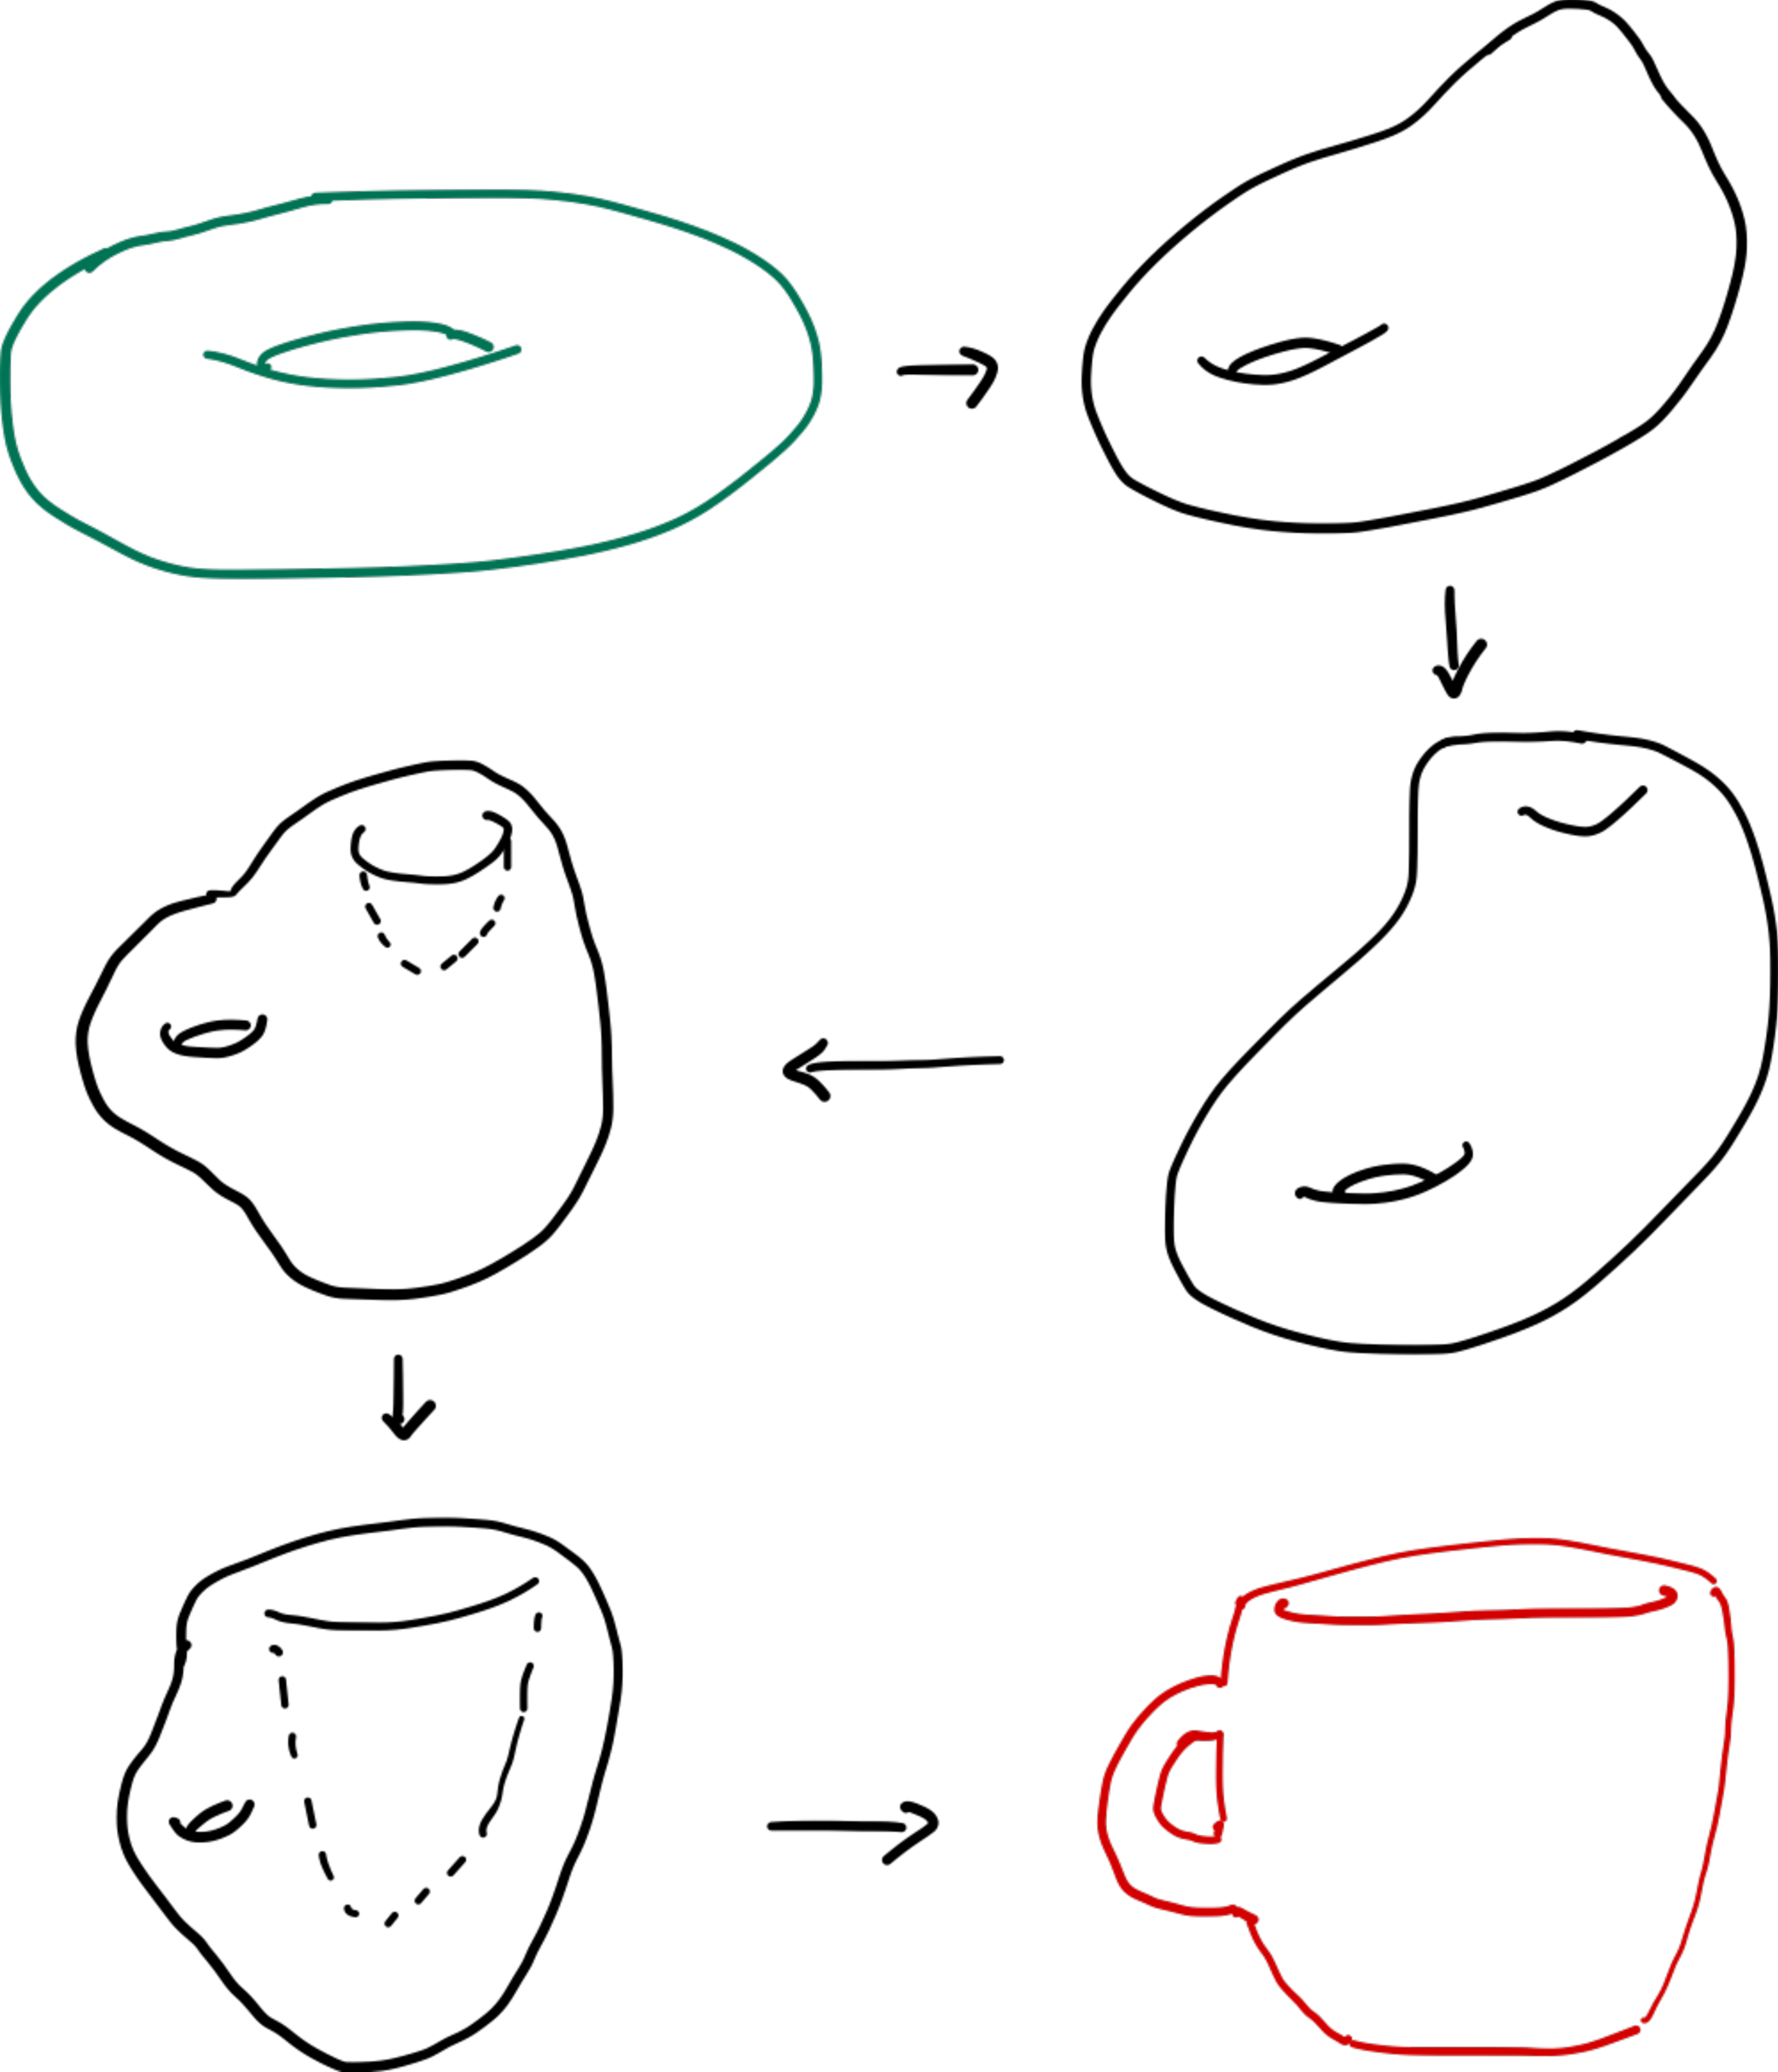
\includegraphics{images/1_1-dount-to-cup.pdf}
  \vspace{5pt}
\end{marginfigure}

\begin{definition}
  A topological space $(X, \cT)$ is \emph{Hausdorff} if every two distinct points admit disjoint open neighbourhoods. That is, for every pair $x\neq y$ of points in $X$, there exist open subsets $U_x, U_y\in\cT$ such that $x\in U_x$, $y\in U_y$ and $U_x \cap U_y = \emptyset$.
\end{definition}

Topological spaces are extremely general, as such they may have very inconvenient---someone may say nasty---properties.
You can see this for yourself with the following exercise.

\begin{exercise}
  \begin{itemize}
    \item Let $X$ be an arbitrary set. Show that $\cT:=\{\emptyset, X\}$ defines a topology on $X$, called the \emph{trivial topology}. Show that on $(X, \cT)$ any sequence in $X$ converges to every point of $X$, and every map from a topological space into $X$ is continuous.
    \item Let $X$ be an arbitrary set. Show that $\cT:=\mathcal{P}(X) := \{ A \mid A\subset X \}$, the powerset of $X$, defines a topology on $X$, called the \emph{discrete topology} in which every map $f : X \to Y$ to some other arbitrary topological space $(Y, \cU)$ is continuous.
  \end{itemize}
\end{exercise}

Hausdorff spaces are still rather general: in particular, any metric space with the metric topology\footnote{Recall that in a metric space $X$ the \emph{metric topology} is defined in the following way: a set $U\subset X$ is called open if for any $x\in U$ there exists $\epsilon>0$ such that $U$ fully contains the ball of radius $\epsilon$ around $x$.} is Hausdorff.

\begin{definition}
  A topological space $(X, \cT)$ is \emph{second countable} if there exists a countable set $\cB\subset\cT$ such that any open set can be written as a union of sets in $\cB$.
  In such case, $\cB$ is called a (countable) basis for the topology $\cT$.
\end{definition}

\begin{exercise}[Euclidean space $\R^n$]\label{exe:rntopsp}
  Let's consider on $\R^n$ the metric topology\footnote{See comment above.} induced by the euclidean metric $d: \R^n \times \R^n \to [0, +\infty)$, $d(x,y) := \sqrt{\sum_{i=1}^n (x^i-y^i)^2}$.
  Show that the topological space defined on $\R^n$ is Hausdorff and second countable.
\end{exercise}

\begin{definition}[Topological manifold]
  A topological space\footnote{From now on, if we say that $X$ is a topological space we are implying that there is a topology $\cT$ defined on $X$.} $M$ is a \emph{topological manifold} of dimension $n$, or topological $n$-manifold, if it has the following properties:
  \marginnote[0.5em]{Note that the finite dimensionality is a somewhat artificial restriction: manifolds can be infinitely dimensional~\cite{book:lang:infinite}. For example, the space of continuous functions between manifolds is a so-called infinite-dimensional Banach manifold.\vspace{1em}}
  \begin{enumerate}[(i)]
    \item $M$ is a Hausdorff space;
    \item $M$ is second countable;
    \item $M$ is \emph{locally euclidean} of dimension $n$, that is\footnote{In words, any point $p\in M$ has a neighbourhood that is homeomorphic to an open subset of $\R^n$.}, for any point $p\in M$ there exist an open subset $U\subset M$ with $p\in U$, and open subset $V\subset\R^n$ and a homeomorphism $\varphi: U\to V$.
  \end{enumerate}
\end{definition}

\begin{notation}
  Reusing the notation of the definition above, we call \emph{(coordinate) chart} the pair $(U, \varphi)$ of a \emph{coordinate neighbourhood} $U$ and an associated \emph{coordinate map}\footnote{Or \emph{coordinate system}.} $\varphi: U\to V$ onto an open subset $V=\varphi(U)\subseteq\R^n$ of $\R^n$.
  Furthermore, we say that a chart is \emph{centred at $p\in U$} if $\varphi(p) = 0$.
\end{notation}

\begin{figure}[htp]
  \centering
  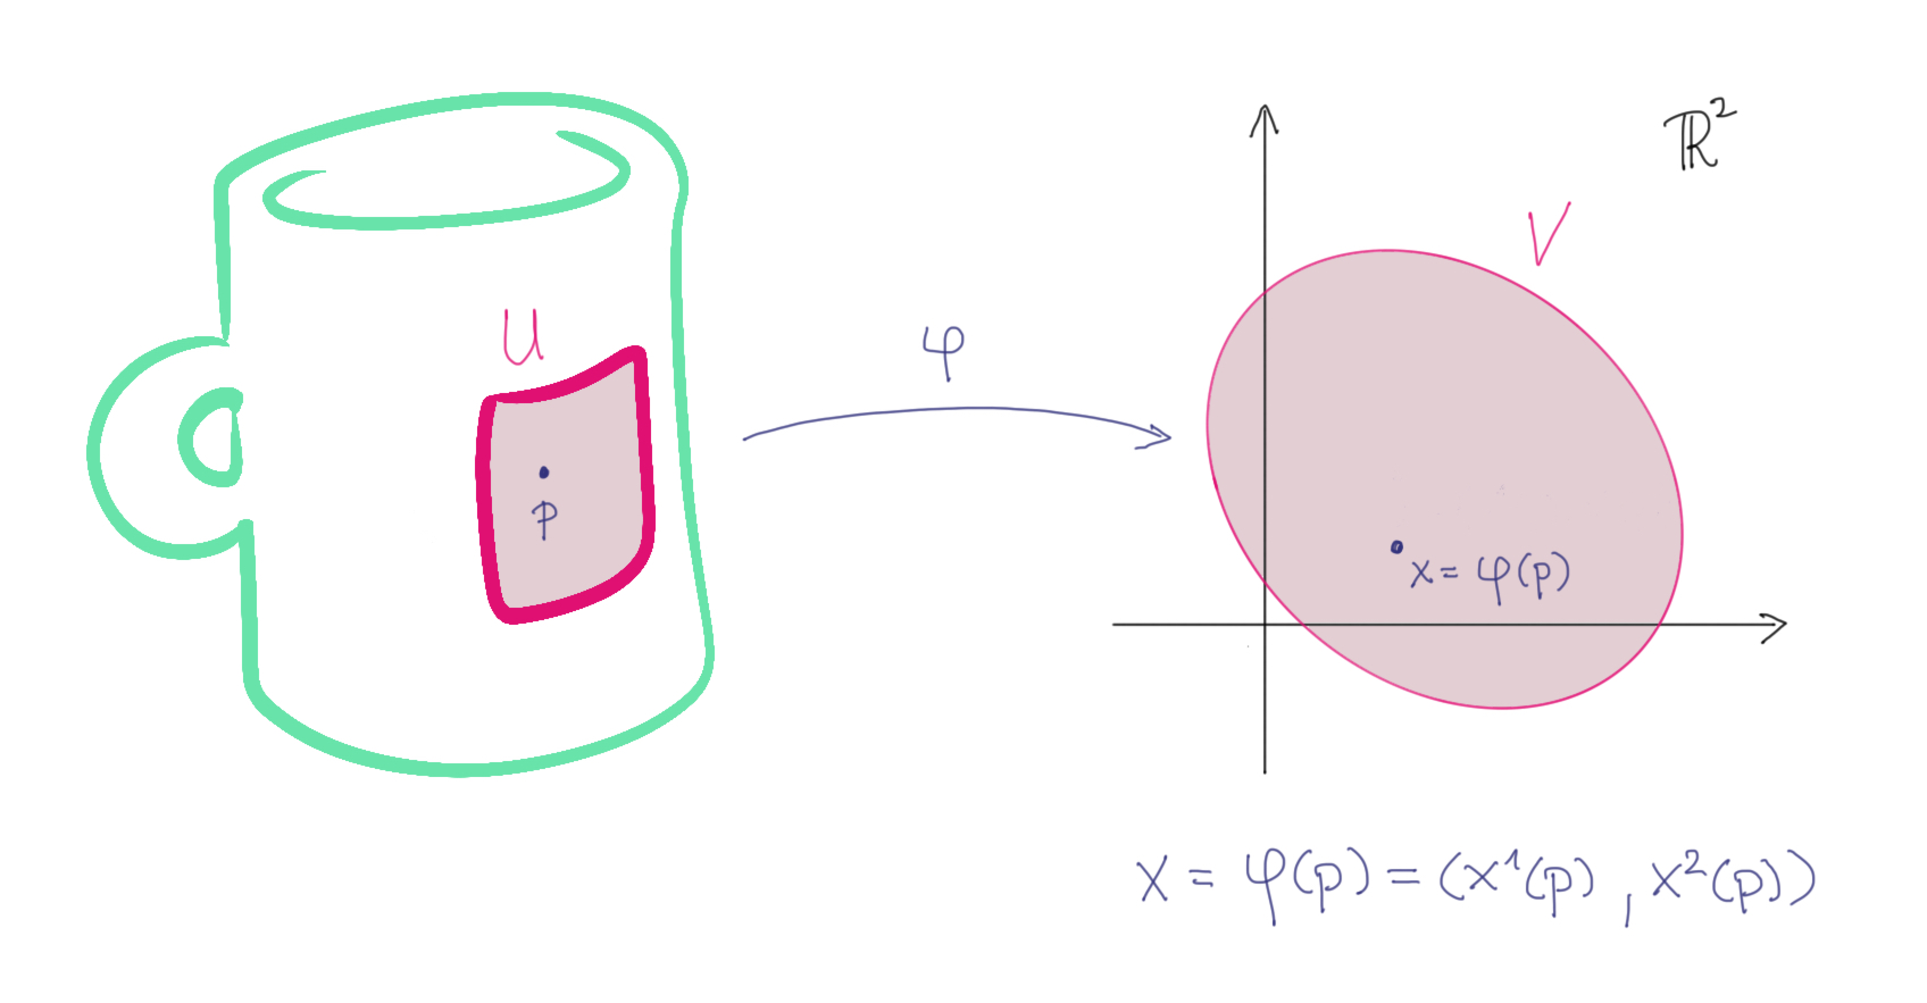
\includegraphics{1_2-charts.pdf}
  \caption{Being locally euclidean allows to define coordinates on the manifold, that is, a mapping between the manifold and the euclidean space.}
  \label{fig:1.2-charts}
\end{figure}

Don't get scared by conditions (i) and (ii) in the definition of topological manifolds: they are only needed to make sure that there are not too few open sets (Hausdorff) and not too many (second countable).

\begin{example}
  With our definition, a countable collections of points with the discrete topology is a $0$-dimensional topological manifold.
  An uncountable collection of points with the discrete topology, however, is not!
\end{example}

\begin{example}
  $\R^n$ is trivially\footnote{Use Exercise~\ref{exe:rntopsp} and the \emph{global} chart $(\R^n, \id_{\R^n})$, where $\id_{\R^n}(x) := x$ is the identity on $\R^n$.} a topological manifold of dimension $n$.
  More generally, any $n$-dimensional vector space\footnote{In fact, any open subset of a $n$-dimensional vector space.} is a topological $n$-manifold.
\end{example}

\begin{exercise}[The line with two origins]
  Even though $\R^n$ with the euclidean topology is Hausdorff, being Hausdorff does not follow from being locally euclidean. A famous counterexample is the following\footnote{See also \cite[Problem 1-1]{book:lee} and \cite[Problem 5.1]{book:tu}.}.
  \begin{marginfigure}
    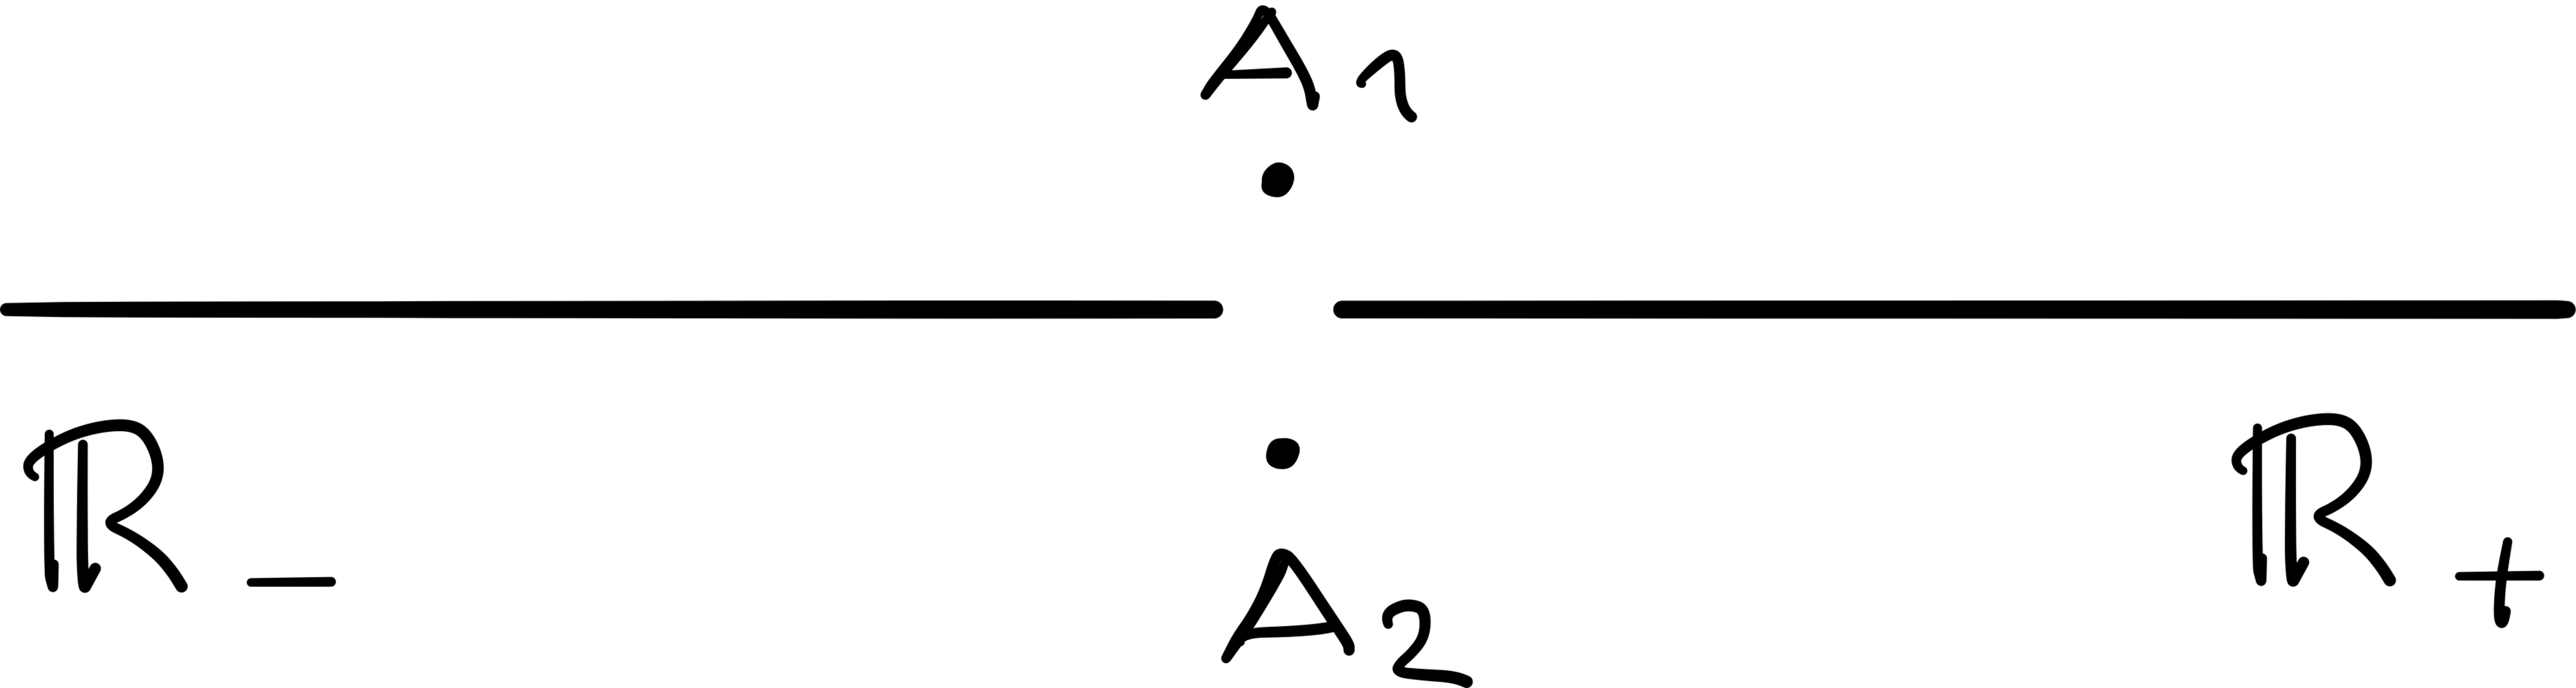
\includegraphics{1_ex_1_0_11.pdf}
    \label{fig:hausdorff-not-locally-euclidean}
    \caption{A locally euclidean space which is not Hausdorff.}
  \end{marginfigure}
  Let $A_1, A_2$ be two points not on the real line $\R$ and define $M:= (\R\setminus\{0\})\cup\{A_1,A_2\}$.
  Induce a topology on $M$ by taking as basis the collection of all open intervals in $\R$ that do not contain $0$, along with all the sets of the form $(-a, 0)\cup\{A_1\}\cup(0,a)$ and $(-a, 0)\cup\{A_2\}\cup(0,a)$, for $a>0$.
  \begin{enumerate}
    \item Check that this forms a basis\footnote{That is, the basis elements cover $M$ and for any $B_1, B_2$ on the basis, for all $x \in I = B_1\cap B_2$, there is an element $B_3$ of the basis such that $x\in B_3$ and $B_3\subset I$.} for a topology on $M$.
    \item Define the two charts
      \begin{equation}
        \varphi_j:(\R\setminus\{0\})\cup\{A_j\} \to \R, \quad
        \varphi_j(x) = \begin{cases} x &\mbox{if } x\neq A_j\\ 0 & \mbox{if } x = A_j \end{cases}, \quad
        j = 1,2.
      \end{equation}
      Show that $\varphi_1$ and $\varphi_2$ are homeomorphisms with respect to the aforementioned topology. 
      %induced by the two charts\footnote{Let $(X, \cT)$ be a topological space and $f: X\to Y$ some map. The induced topology on $Y$ is \begin{equation}\cU_f := \{f^{-1}(U) \;\mid\; U\in\cT\}.\end{equation}}.
    \item Show that $M$ is locally euclidean and second countable but not Hausdorff.
  \end{enumerate}
\end{exercise}

\begin{example}\label{ex:uball}
  The \emph{closed} unit ball $D_1(0)$, where similarly as before
  \begin{equation}
    D_r(x) := \{z\in\R^n \;\mid\; d(z,x) \leq r\},
  \end{equation}
  is \emph{not} a topological manifold of dimension $n$. Can you see why? In fact, this is an example of a more general concept of \emph{manifold with boundary} that we will introduce later in Chapter~\ref{sec:mbnd}.
\end{example}

\begin{example}
  Consider the set $M := \{ x\in\R^2 \;\mid\; |x^1| = |x^2| \}$ with the topology induced by $\R^2$:
  this is \emph{not} a topological manifold.
  Since the number of connected components is invariant under homeomorphisms, open connected neighbourhoods of $(0,0)\in M$ cannot be\footnote{A drawing of $M$ is worth more than a hundred words.} homeomorphically mapped to open connected sets in $\R$.
\end{example}

\newthought{There is still an elephant in the room} in need of a comment.
In our definition of topological manifolds, we are taking for granted that the dimension of the manifold is well--defined, that is, if we have two different charts, $\varphi_1: U \to \R^n$ and $\varphi_2: U \to \R^m$, then necessarily $m=n$. Luckily this is true! The result is called \emph{Invariance Domain Theorem} and, since its proof requires advanced concepts of algebraic topology, we will not pursue it further in the course.
\marginnote[-2em]{There is a caveat, the theorem holds for \emph{connected} components of a manifold. If you consider two distinct connected components, you can indeed have different dimensions for each of them.}

\section{Differentiable manifolds}

Before entering into the details of new definitions, let's recall what will be the most important tools throughout the rest of the course.

\begin{definition}
  A map $f: U \to V$ between open sets $U\subset\R^n$ and $V\subset\R^m$ is in $C^r(U,V)$ or \emph{of class $C^r$}, if it is continuously differentiable $r$-times.
  It is called a $C^r$-\emph{diffeomorphism}\footnote{With this definition a homeomorphism is a $C^0$-diffeomorphism} if it is bijective and of class $C^r$ with inverse of class $C^r$.
  We say that $f$ is \emph{smooth}, or of class $C^\infty$, if it is of class $C^r$ for every $r \geq 1$.
\end{definition}

\begin{theorem}[Chain rule]\label{thm:chainrule}
  Let $U\subset\R^n$ and $V\subset\R^k$ be open sets and $f: U \to \R^k$, $g: V\to\R^m$ two continuously differentiable functions such that $f(U)\subset V$.
  Then, the following holds.
  \begin{enumerate}[(i)]
    \item\label{thm:chainrule1} The function $g\circ f: U\subset\R^n \to\R^m$ is continuously differentiable and its total derivative~\eqref{eq:jacobian} at a point $x\in U$ is given by
      \begin{equation}
        D(g\circ f)(x) = (Dg)(f(x)) \circ Df(x).
      \end{equation}
    \item\label{thm:chainrule2} Denote $x=(x^1, \ldots, x^n)\in\R^n$ and $y=(y^1,\ldots,y^k)\in\R^k$ the coordinates on the respective euclidean spaces and $f=(f^1,\ldots,f^k)$ and $g=(g^1,\ldots,g^m)$ the components of the functions. Then the partial derivatives of $g\circ f$ are given by
      \begin{equation}
        \frac{\partial g^i\circ f}{\partial x^j}(x)
        = \sum_{r=1}^k \frac{\partial g^i}{\partial y^r}(f(x)) \frac{\partial f^r}{\partial x^j}(x),
        \qquad 1\leq i \leq m,\; 1\leq j\leq n.
      \end{equation}
  \end{enumerate}
\end{theorem}
\marginnote[-5em]{Using Einstein's notation, this could be written as \begin{equation}\frac{\partial (g^i\circ f)}{\partial x^j}(x) = \frac{\partial g^i}{\partial y^r}(f(x)) \frac{\partial f^r}{\partial x^j}(x).\end{equation}}

Theorem~\ref{thm:chainrule} has some very deep consequences.
\begin{exercise}
  Under the hypotheses of the previous theorem, prove the following statements.
  \begin{enumerate}
    \item composition preserves the regularity: that is, the composition of functions of class $C^r$ is itself a function of class $C^r$;
    \item if $f:U\subset\R^n\to V\subset\R^m$ is a diffeomorphism, then $n=m$.
  \end{enumerate}
  \textit{\small Hint: is $Df(x)$ an invertible matrix? If so, what is its inverse?} %$D(f^{-1})(f(x))$.
\end{exercise}

Since differentiability is a \emph{local} property and topological manifolds are \emph{locally} like euclidean spaces, it seems reasonable to expect that we can lift the definitions directly from $\R^n$ using the charts to obtain functions between euclidean spaces:
for example, if we are given a continuous map between two topological manifolds, we can locally view it as a continuous map between two euclidean spaces.
Generalizing this further, we could conceivably say that our original map is differentiable if the local map is.

\newthought{As usual, the devil is in the details}: a topological manifold is only homeomorphic to a euclidean space, and a different choice of homeomorphism might affect whether the local map is differentiable or not.
We need to take extra care to ensure that these lifted definitions keep making sense when we use different charts that overlap.

The solution is to introduce a little more structure to the problem.

\begin{definition}\label{def:crcomp}
  We say that two charts $(U_1, \varphi_1)$ and $(U_2, \varphi_2)$ on a topological manifold $M$ are \emph{compatible} if either $U_1 \cap U_2 = \emptyset$ or if the \emph{transition map}\footnote{Both the composition maps $\varphi_1 \circ \varphi_2^{-1}$ and $\varphi_2 \circ \varphi_1^{-1}$ are called transition maps. Both maps are necessarily homeomorphisms since $\varphi_1$ and $\varphi_2$ are.}
  \begin{equation}
    \varphi_1 \circ \varphi_2^{-1} : \varphi_2(U_1\cap U_2) \to \varphi_1(U_1 \cap U_2)
  \end{equation}
  is a smooth diffeomorphism.
\end{definition}

\begin{figure*}[htp]
  \centering
  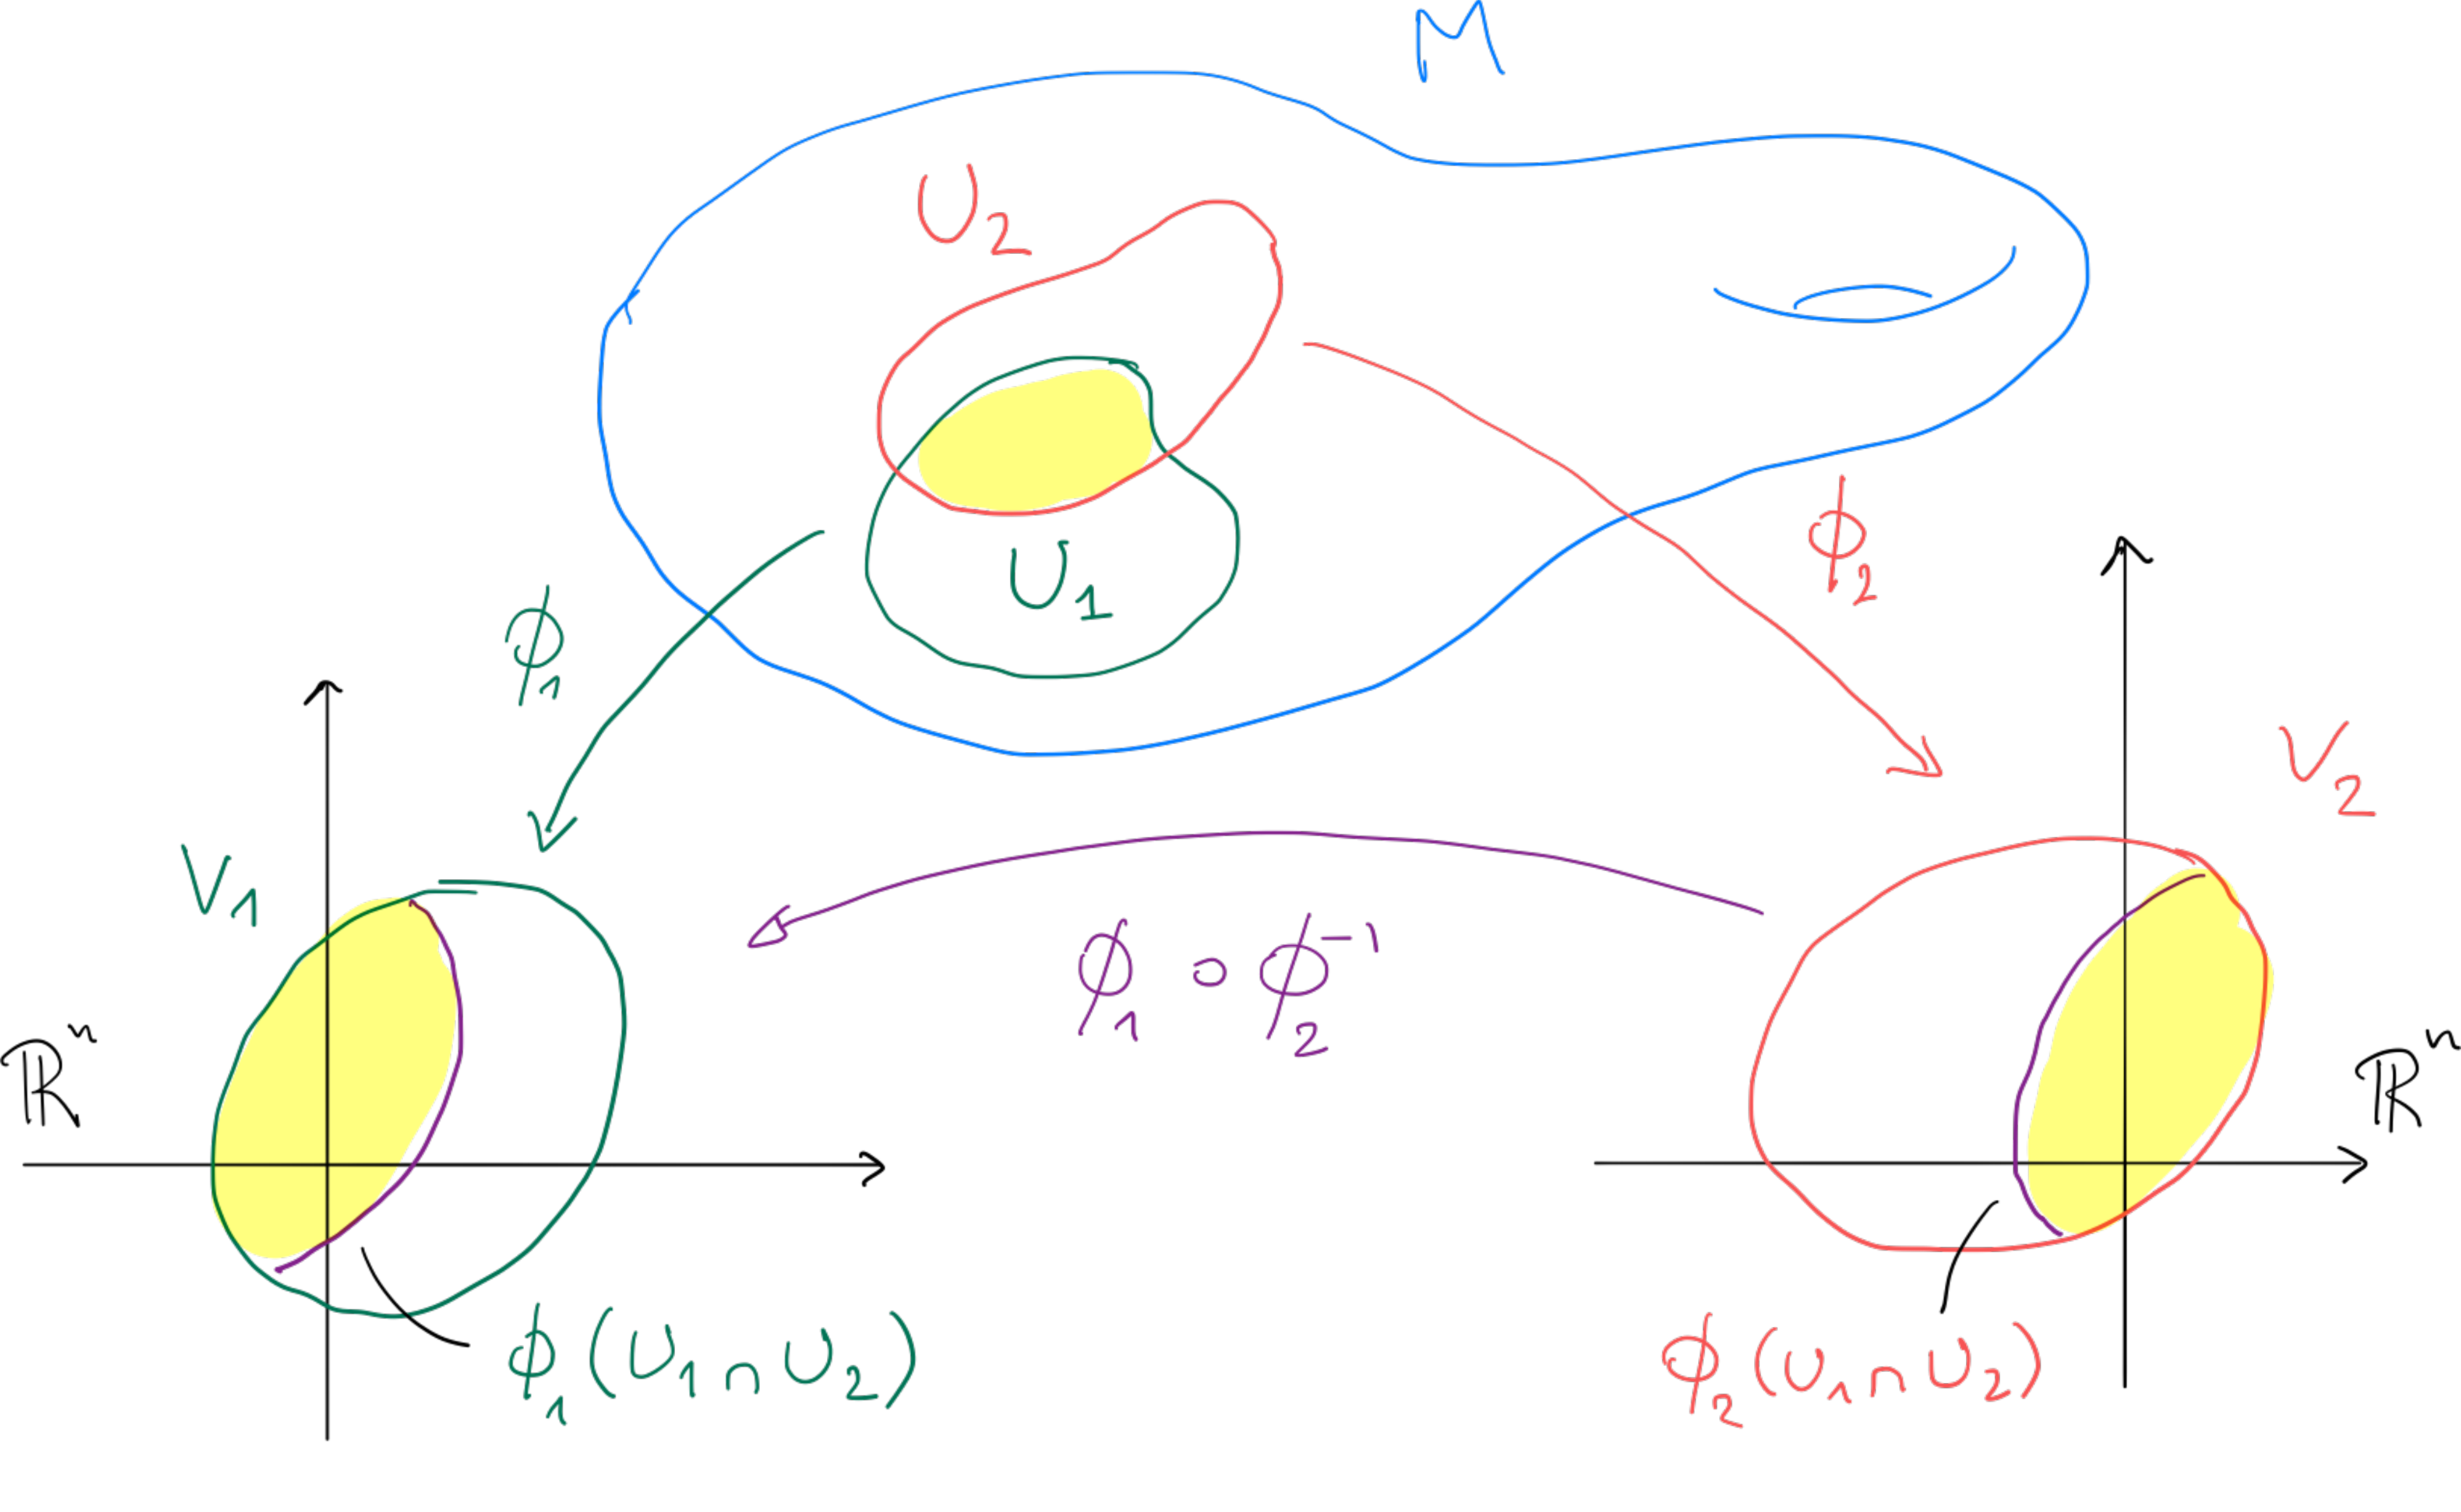
\includegraphics{1_2-compatible-charts.pdf}
  \caption{Charts are compatible if they coincide on the intersections of their coordinate neighbourhoods.}
  \label{fig:1.2-compatible-charts}
\end{figure*}

With these at hand, let's jump into the definition of smooth manifolds.

\begin{definition}\label{def:cratlas}
  A \emph{smooth atlas} is a collection
  \begin{equation}
    \cA = \{\varphi_\alpha: U_\alpha \to V_\alpha \;\mid\; \alpha\in A\}
  \end{equation}
  of pairwise compatible charts that cover\footnote{I.e. such that $M = \cup_{\alpha\in A} U_\alpha$. One calls the set $\{U_\alpha \;\mid\; \alpha\in A\}$, covering $M$ with open sets, an \emph{open cover} of $M$. Here $A$ is some index set, not necessarily countable.} $M$.

  Two smooth atlases are \emph{equivalent} if their union is also a smooth atlas. That is if any two charts in the atlases are compatible.
\end{definition}

\begin{exercise}
  Show that the equivalence of atlases is really an equivalence relation.
\end{exercise}

\begin{definition}\label{def:diffstr}
  \marginnote{The union of all atlases in a differentiable structure is the \emph{unique} \emph{maximal} atlas in the equivalence class.
  There is a one-to-one correspondence between differentiable structures and maximal differentiable atlases \cite[Proposition 1.17]{book:lee}: for convenience and to lighten the notation, from now on, we will always regard a differentiable structure as a differentiable maximal atlas without further comments.}
  A \emph{differentiable structure}, or more precisely a \emph{smooth structure}, on a topological manifold is an equivalence class of smooth atlases.
\end{definition}

\begin{notation}
  By a \emph{chart $(U, \varphi)$ about $p$} in a manifold $M$ we mean a chart in the differentiable structure of $M$ such that $p\in U$.
\end{notation}

\begin{definition}\label{def:diffmanifold}
  A \emph{smooth manifold} of dimension $n$ is a pair $(M, \cA)$ of a topological $n$-manifold $M$ and a smooth structure $\cA$ on $M$.
  \marginnote[1em]{There are no preferred coordinate charts on a manifold: all coordinate systems compatible with the differentiable structure are on equal footing.}
\end{definition}

In colloquial language, a differentiable manifold is just a space covered by charts with differentiable transition maps.
Note that not all topological manifolds can be made into smooth manifolds, but counterexamples are hard to construct and you need at least to go to dimension 4.
A nice and super compact explanation with the relevant reference is in \cite{SE2691140}.

\begin{notation}
  Whenever possible we will omit the differentiable structure $\cA$ from the notation and just write $M$.
  We may write $M^n$ when we want to emphasize that the dimension of $M$ is $n$.
\end{notation}

\begin{exercise}
  Show that on a second countable differentiable manifold it is always possible to find a countable atlas.
\end{exercise}

\begin{exercise}\label{exe:subsetsmanifolds}
  $\R^n$ with the \emph{standard} smooth structure $\cA=\{(\R^n, \id_{\R^n})\}$ is trivially a smooth manifold of dimension $n$.
  %
  In fact, any open subset $U\subset\R^n$ can be made into a smooth manifold in a natural way with the atlas $\cA=(U, \id_{\R^n}|_U)$.

  In the same way, show that any open subset $U$ of a smooth manifold $M$ is a smooth manifold.
  Which atlas would you choose?

  More generally, if $V$ is any $n$-dimensional real vector space, then the standard smooth structure on $V$ is the one induced by the smooth atlas consisting of a single chart $(V, T)$ where $T: V \to \R^n$ is some linear isomorphism.
  Why is this independent of the choice of the isomorphism $T$?

  This fact has a very interesting consequence.
  The space $\mathrm{Mat}(n, \R)$ of real $n\times n$-matrices can be identified with $\R^{n^2}$ by writing the elements of the matrix as a $n^2$-vector.
  This gives to $\mathrm{Mat}(n, \R)$ a structure of differentiable manifold.
  The subset of invertible matrices $GL(n) := GL(n, \R) = \{ A \in \mathrm{Mat}(n, \R) \;\mid\; \det A \neq 0\}$, widely known as the \emph{general linear group}, being an open subset of $\mathrm{Mat}(n, \R)$ (why?) is itself a differentiable manifold.
  Is such manifold connected? Why?
\end{exercise}

\vspace{1em}
\begin{notation}\label{ntn:coords}
  We will stick to the notation of~\cite{book:tu}.
  In the context of manifolds, denote $r^i: \R^n\to\R$, $1\leq i\leq n$, the standard coordinates on $\R^n$.
  With this notation, if $e_i$ denotes the $i$th standard basis vector\footnote{Identified with the \emph{point} $(0,\ldots,0,\LaTeXunderbrace{1}_{i\mbox{th component}},0,\ldots,0) \in\R^n$.} in $\R^n$, then $r^i(e_j) = \delta^i_j$.
  \marginnote{The Kronecker delta $\delta_j^i$ is defined by $\delta_j^i = 1$ if $i=j$ and $\delta_j^i = 0$ otherwise.}

  If $(U, \varphi:U\to\R^n)$ is a chart of a manifold, then $x^i = r^i\circ\varphi$ will denote the $i$-th component of $\varphi$ and denote $\varphi = (x^1, \ldots, x^n)$ and, when convenient, $(U,\varphi) = (U, x^1, \ldots, x^n)$ (see also Figure~\ref{fig:1.2-charts}).

  Thus, for $p\in U$, $(x^1(p), \ldots, x^n(p))$ is a point\footnote{By abuse of notation we sometimes omit the $p$. 
  Thus $(x^1, \ldots, x^n)$ can stand either for local coordinates or a point in $\R^n$: which one it is should be clear from the context.} in $\R^n$.
  The functions $x^1, \ldots, x^n$  are called \emph{(local) coordinates} on $U$.
\end{notation}
\vspace{1em}

An advantage of this new notation is that we can talk about coordinates without the need to explicitly reference charts. In other words, we can say
\begin{quote}
  Let $p\in M$ and choose local coordinates $(x^1, \ldots, x^n)$ about $p$...
\end{quote}
or even
\begin{quote}
  Let $x=(x^1, \ldots, x^n)\in M$ be a point in $M$...
\end{quote}
dropping the distinction between $p$ and $x$, both in place of
\begin{quote}
  Let $p \in M$ and $(U, \varphi)$ a chart defined on a neighbourhood $U$ of $p$.
  Let $x^i = r^i \circ\varphi$ denote the components of $\varphi$ with respect to the standard euclidean coordinates\ldots
\end{quote}

\begin{example}\label{ex:S1emb}
  The unit circle
  \begin{equation}
    \bS^1 := \{x\in\R^2 \;\mid\; \|x\|=1\}\subset\R^2
  \end{equation}
  with the relative topology\footnote{Let $(X,\cT)$ be a topological space and $Y\subset X$. The \emph{relative topology} on $Y$ is \begin{equation}\mathcal{V}:=\{V\subset Y\;\mid\;\exists U\in\cT \mbox{ s.t. } V = U \cap Y\}.\end{equation}} is a $1$-dimensional topological manifold.
  To provide the local homeomorphisms to $\R$ and define a smooth structure for $\bS^1$ it is enough to define the following four charts:
  \begin{equation}
    \begin{aligned}
      &V_1 := \{ x^1 > 0 \},\quad \varphi_1: V_1 \to (-1, 1), \quad \varphi_1(x) := x^2,\\
      &V_2 := \{ x^1 < 0 \},\quad \varphi_2: V_2 \to (-1, 1), \quad \varphi_2(x) := x^2,\\
      &V_3 := \{ x^2 > 0 \},\quad \varphi_3: V_3 \to (-1, 1), \quad \varphi_3(x) := x^1,\\
      &V_4 := \{ x^2 < 0 \},\quad \varphi_4: V_4 \to (-1, 1), \quad \varphi_4(x) := x^1.
    \end{aligned}
  \end{equation}
  What do these charts look like?
\end{example}
\begin{exercise}
  In the previous example, show that the corresponding transition functions are smooth.
\end{exercise}

\begin{exercise}
  Let $\{(U_\alpha, \varphi_\alpha)\}$ be the maximal atlas on a manifold $M$.
  For any open set $U\subseteq M$ and any point $p\in U$, prove the existence of a coordinate open set $U_\alpha$ such that $p\in U_\alpha\subset U$.
\end{exercise}

\begin{exercise}
  Let $f: \R^n \to \R^m$ be a smooth map.
  Show that its graph
  \begin{equation}
    \Gamma_f := \{(x, f(x)) \;\mid\; x\in\R^n\} \subset\R^{n+m}
  \end{equation}
  is a smooth manifold of dimension $n$.
\end{exercise}

\begin{example}
  The definition of smooth manifold does not require $M$ to be embedded into some ambient space as in the examples above.
  In fact, we can define the differentiable manifold $\bS^1$ by equipping the topological quotient space\sidenote[][-11em]{
    There is a standard way to induce a topology on a quotient space.
    Let $M$ be a topological space and $\pi:M\to N$ surjective.
    The \emph{quotient topology} on $N$ is given by defining $U\subset N$ to be open if and only if its preimage $\pi^{-1}(U)\subset M$ is open.
    If $\sim$ is an equivalence relation on $M$, the quotient space $M/\!\sim$ is the set of equivalence classes $[p]:=\{q\in M \mid p\sim q\}$ and the projection $\pi: M\to M/\!\sim$, $\pi(p) = [p]$, is a surjective map. Then $U\in M/\!\sim$ is open if $\cup_{[p]\in U} [p] \subset M$ is open.
    Here $\R/\Z$ denotes the quotient space $\R/\!\sim$ where the equivalence relation is induced by the canonical group action of $\Z$ on $\R$, that is, $x\sim y$ if and only if $x-y\in\Z$.
    This means that $[x] = \{x+k \mid k\in\Z\}$ and each interval $[x_0, x_0+1)$ of length $1$ contains exactly one representative per class.
  Note that we are talking about topological spaces: the quotient, in general, does not preserve the Hausdorff property or second countability.} $\R/\Z$ with the two charts
  \begin{equation}\textstyle
    \varphi_1 : \R/\Z \setminus\{[0]\} \to (0,1)
    \quad\mbox{and}\quad
    \varphi_2 : \R/\Z \setminus\{[\frac12]\} \to (-\frac12,\frac12)
  \end{equation}
  which map $[x]\in\R/\Z$ to its representation in $[0,1)$ or $[-\frac12, \frac12)$ respectively.
  The manifold obtained in this way is diffeomorphic to the one defined in Example~\ref{ex:S1emb}.
\end{example}

\begin{example}[Product manifolds]\label{ex:pm}
  Given two manifolds $(M_1, \cA_1)$ and $(M_2, \cA_2)$, we can define the \emph{product manifold} $M_1 \times M_2$ by equipping $M_1 \times M_2$ with the product topology\footnote{Open sets in the product are products of open sets from the respective topological spaces.} and covering the space with the atlas $\{ (U_1\times U_2, (\varphi_1, \varphi_2)) \;\mid\; (U_1, \varphi_1)\in\cA_1, (U_2, \varphi_2)\in \cA_2\}$.
\end{example}

Note that smooth manifolds do not yet have a metric structure: distances between the points are not defined.
However, they are \emph{metrizable}\footnote{In fact, all the topological manifolds are metrizable. This property is far more general and harder to prove~\cite[Theorem 34.1 and Exercise 1 of Chapter 4.36]{book:munkres:topology} or \cite{nlab:urysohn_metrization_theorem}. Note that not all topological spaces are metrizable, for example a space with more than one point endowed with the discrete topology is not. And even if a topological space is metrizable, the metric will be far from unique: for example, proportional metrics generate the same collection of open sets.}: there exists some metric on the manifold that induces the given topology on it.
This allows to always view manifolds as metric spaces.

Instead of always constructing a topological manifold and then specify a smooth structure, it is often convenient to combine these steps into a single construction.
This is especially useful when the initial set is not equipped with a topology.
In this respect, the following lemma provides a welcome shortcut: in brief it says that given a set with suitable ``charts'' that overlap smoothly, we can use those to define both a topology and a smooth structure on the set.

\begin{lemma}[Smooth manifold lemma]\label{lem:manifold_chart}
  Let $M$ be a set. Assume that we are given a collection $\{U_\alpha\mid \alpha\in A\}$ of subsets of $M$ together with bijections $\varphi_\alpha: U_\alpha\to\varphi(U_\alpha)\subseteq\R^n$, where $\varphi(U_\alpha)$ is an open subset of $\R^n$. Assume in addition that the following hold:
  \begin{enumerate}[(i)]
    \item For each $\alpha, \beta \in A$, the sets $\varphi_\alpha(U_\alpha \cap U_\beta)$ and $\varphi_\beta(U_\alpha \cap U_\beta)$ are open in $\R^n$.
    \item If $U_\alpha \cap U_\beta \neq \emptyset$, the map $\varphi_\beta\circ\varphi_\alpha^{-1}: \varphi_\alpha(U_\alpha \cap U_\beta)\to \varphi_\beta(U_\alpha \cap U_\beta)$ is smooth.
    \item Countably many of the sets $U_\alpha$ cover $M$.
    \item If $p\neq q$ are points in $M$, either there exists $\alpha$ such that $p,q\in U_\alpha$ or there exist $\alpha,\beta$ with $U_\alpha\cap U_\beta=\emptyset$ such that $p\in U_\alpha$ and $q\in U_\beta$.
  \end{enumerate}
  Then $M$ has a unique smooth manifold structure such that each $(U_\alpha,\varphi_\alpha)$ is a smooth chart.
\end{lemma}
\begin{exercise}
  Prove Lemma~\ref{lem:manifold_chart}.\\
  \textit{\small Hint: declare all the $\varphi_\alpha$ to be homeomorphisms and use the hypotheses to check the definition of a smooth manifold.}
\end{exercise}

\begin{example}
  Lemma~\ref{lem:manifold_chart} simplifies life a lot.
  Consider the product manifolds from Example~\ref{ex:pm}.
  Since both $M$ and $N$ are smooth manifolds, the product manifold is a $(m+n)$-dimensional smooth manifold with the atlas introduced in the example.

  The proof of this fact is trivial in the sense that each of the maps in the atlas satisfies all the properties of the lemma by construction, after all they are already part of the differentiable structure of a smooth manifold.
\end{example}

\begin{exercise}
  Prove that the $n$-dimensional torus
  \begin{equation}
    \bT^n := \LaTeXunderbrace{\bS^1\times\cdots\times\bS^1}_{n\mbox{ times}} \subset \R^{2n}
  \end{equation}
  is a smooth manifold of dimension $n$.
\end{exercise}

\subsection{Quotient manifolds}

If $M$ is a topological space and $\sim$ an equivalence relation we have seen that it is sometimes possible to define smooth manifolds.
Since in general the quotient does not behave nicely it is convenient to get a few tricks to check if the manifold structure can be preserved.

In this case it is convenient to have some tools to check continuity of functions.

\begin{proposition}
\marginnote{For a proof refer to \cite[Proposition 7.1]{book:tu} or \cite[Theorem 3.70]{book:lee:topology}.}
  Assume $F:X\to Y$ is a map between topological spaces and $\sim$ is an equivalence relation on $X$.
  Let $F$ be constant on each equivalence class $[p]\in X/\!\sim$, and denote $\widetilde F:X/\!\sim\to Y$, $\widetilde F([p]) := F(p)$ for $p\in X$, the map induced by $F$ on the quotient.

  Then, $\widetilde F$ is continuous if and only if $F$ is continuous.
\end{proposition}

Continuity of the projection $\pi: M \to M/\!\sim$ implies that if $M/\!\sim$ is Hausdorff, then $\pi^{-1}(\pi(s)) = [s]$ is closed in $M$.
If, additionally, $\pi$ is open\footnote{That is, it maps open sets to open sets.} then there is a stronger statement:
\marginnote[4em]{These statements are not hard to prove, but their proofs will be omitted here.
You can refer to~\cite[Chapters 7.1--7.5]{book:tu}.}
\begin{theorem}\label{thm:openproj}
  If $M$ is a topological space and $\sim$ an equivalence relation such that $\pi:M \to M/\!\sim$ is open, then:
  \begin{itemize}
    \item $\pi$ maps a basis for the topology of $M$ into a basis for the topology $M/\!\sim$, thus if $M$ is second countable, then $M/\!\sim$ is second countable;
    \item the quotient space $M/\!\sim$ is Hausdorff if and only if the graph $R$ of $\sim$, i.e., the set
      \begin{equation}
        R := \{(x,y)\in M\times M \mid x\sim y\},
      \end{equation}
      is closed in $M\times M$.
  \end{itemize}
\end{theorem}

In general, however, the class of quotient space is too large to admit a good general theory of smooth manifolds.
Yet, there is a family of manifolds that has undergone lots of research and on which a lot can be said: smooth manifolds with certain smooth Lie group actions.
Treating this will be far too much for the course, but we will provide along the way most of the necessary ingredients for you to be able to explore the topic on your own.
For further reference, you can look at~\cite[Chapter 21]{book:lee}.

Before moving on, below we are going to look at a couple of simpler, notable, examples of quotient manifolds.

\begin{example}
  Let $\RP^n$ denote the $n$-dimensional real projective space, that is, the space of lines in $\R^{n+1}$ passing through the origin.
  This is a notable example of quotient manifold: we are going to show that $\RP^n$ is a smooth manifold of dimension $n$. 

  We can define an equivalence relation on $\R^{n+1}_0:=\R^{n+1}\setminus\{0\}$ by declaring that for any $x,y\in \R^{n+1}_0$
  \begin{equation}
    x\sim y \quad\Longleftrightarrow\quad \exists t\neq 0 \mbox{ such that } y=tx,
  \end{equation}
  that is, two points are equivalent if they lie on the same line passing through the origin.
  Then, the \emph{real projective space} is the quotient space $\RP^n := \R^{n+1}_0/\!\sim$.
  For the sake of the example, let's denote the class of equivalence of a point $x=(x^0,\ldots,x^n)\in\R^{n+1}_0$ by $[x]=[x^0,\ldots,x^n]$ and the projection to the quotient by $\pi:\R^{n+1}_0\to\RP^n$.
  The classes of equivalence $[x]$ are called \emph{homogeneous coordinates} on $\RP^n$.

  \begin{marginfigure}
    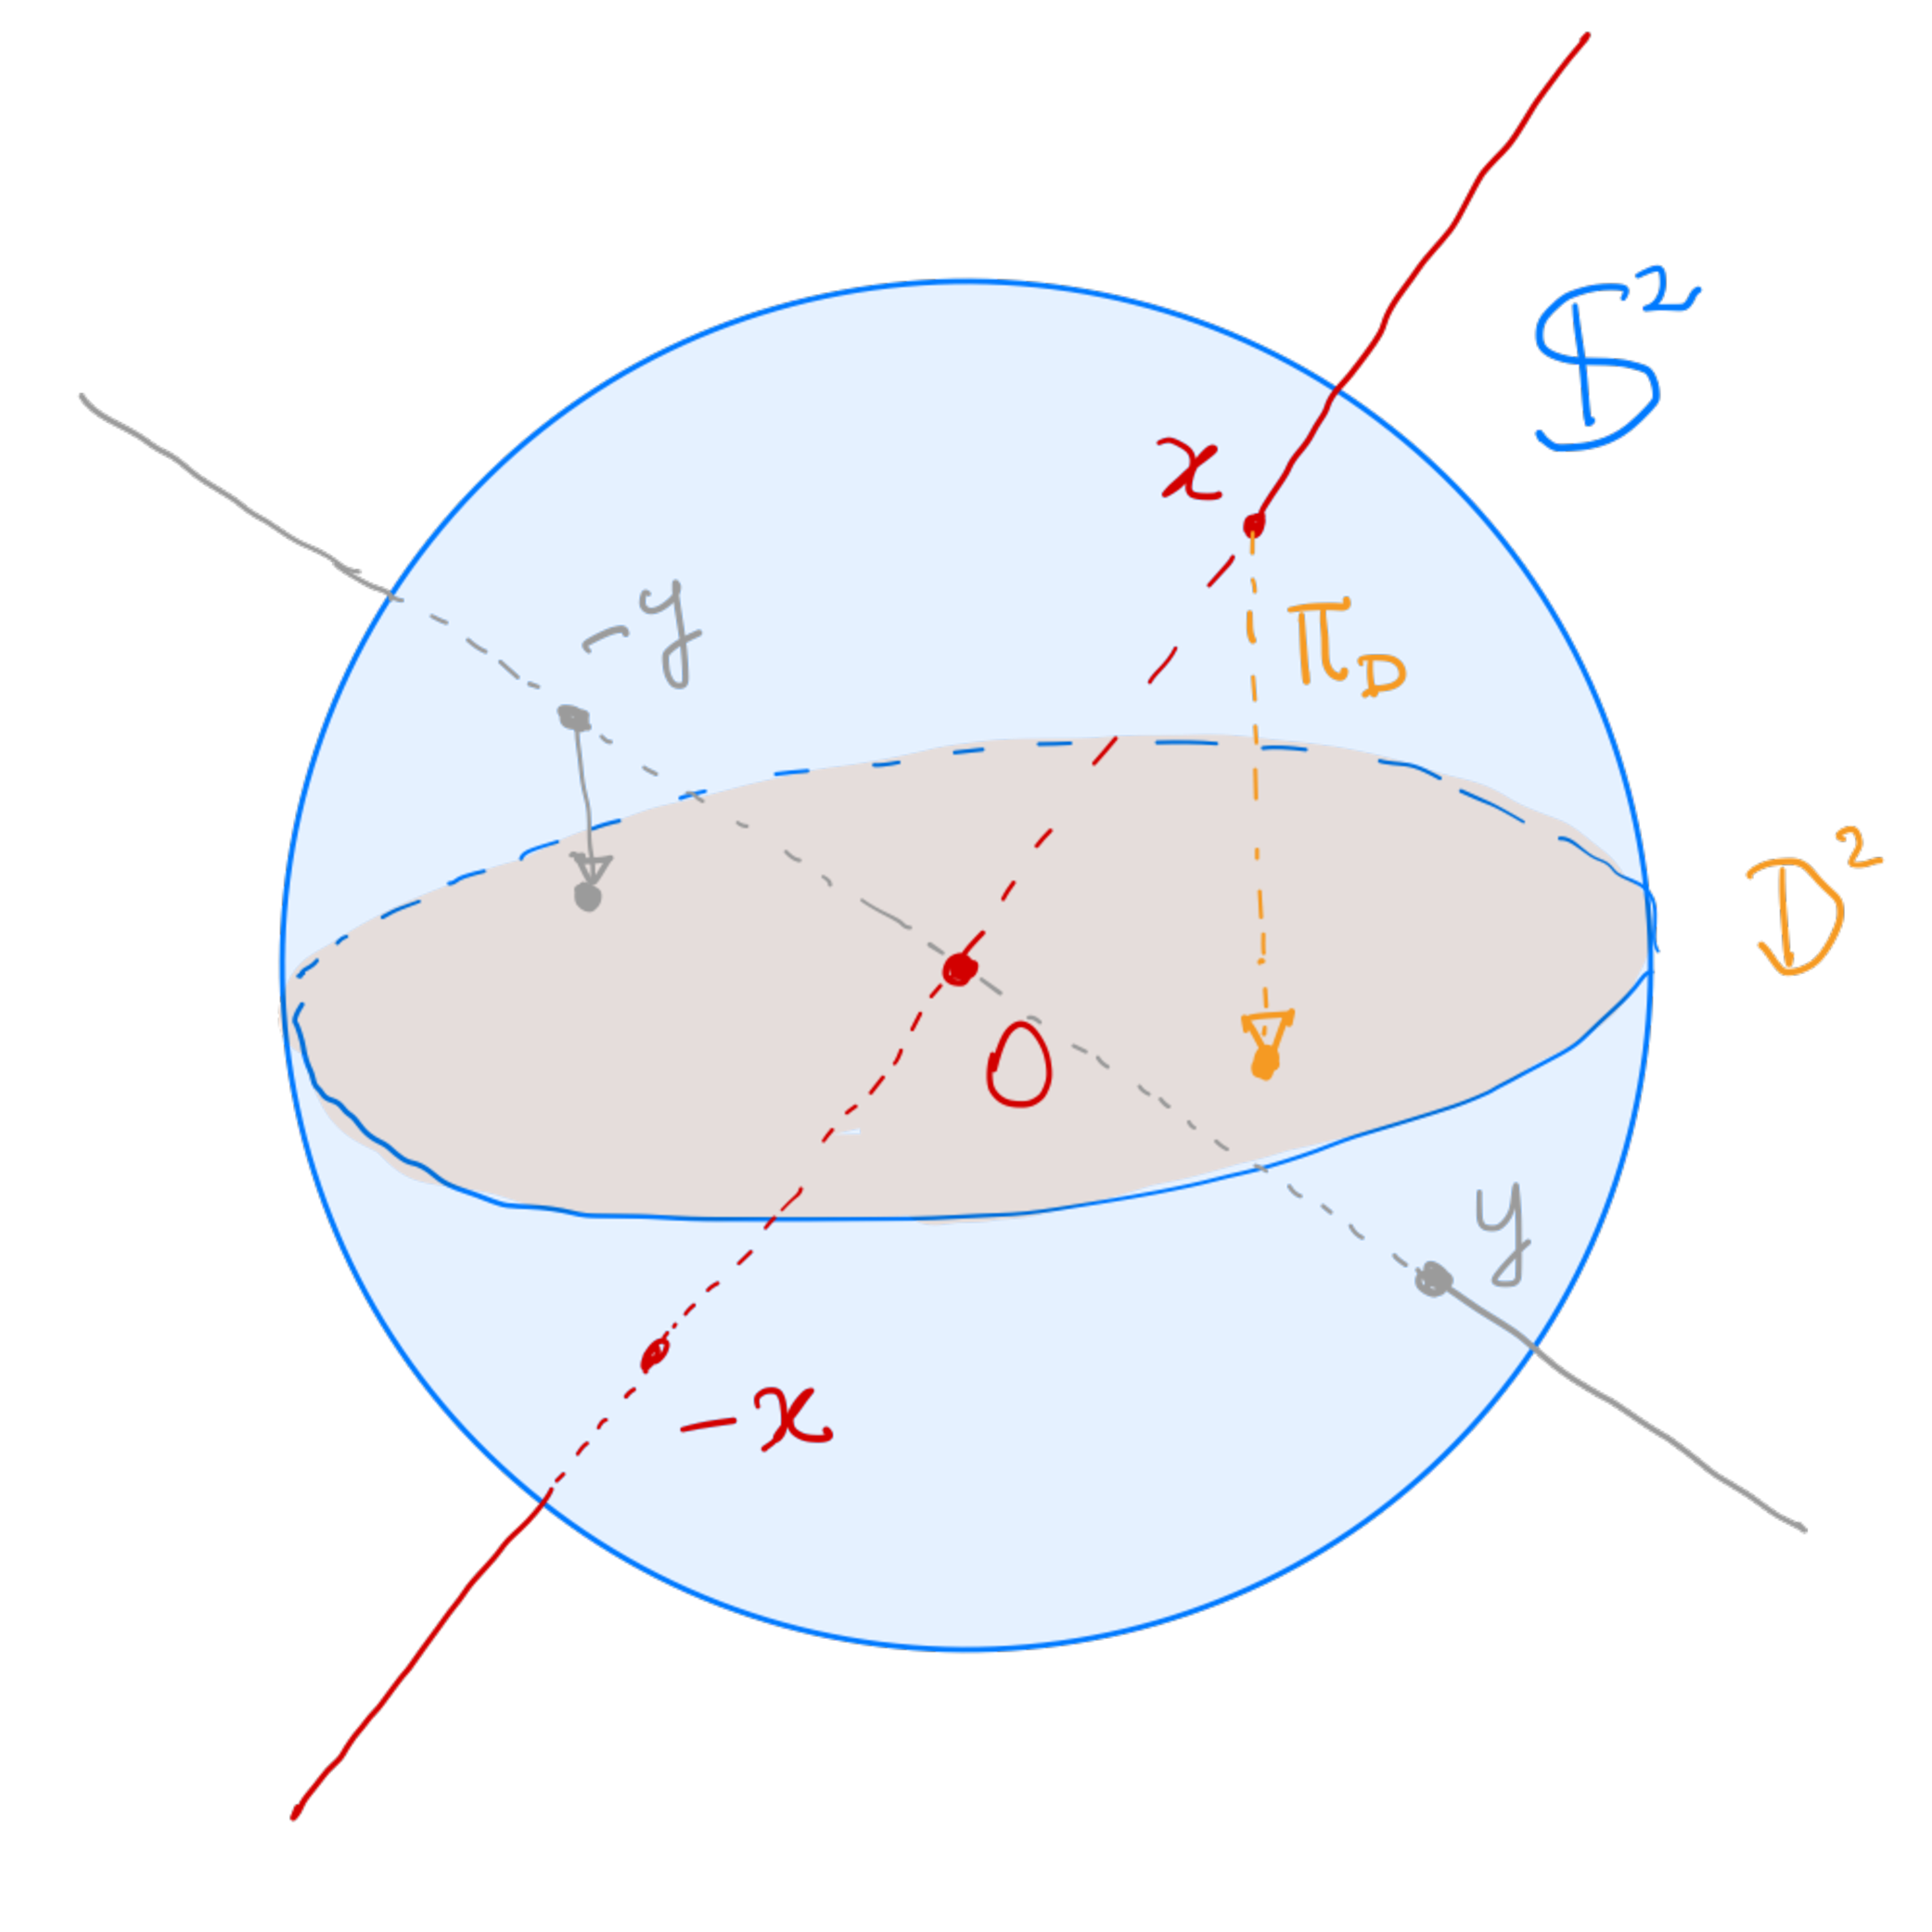
\includegraphics{1_2_25-sphere}
    \caption{The identification $\sim'$ of antipodal points maps the sphere to a disk. Embedding $\bS^n/\!\sim'$ in $\R^{n+1}$, one can define a map $\pi_D$ that projects the representative of $[x]$ in the north hemisphere orthogonally to the disk $D^n = \{x\in\R^{n+1} \mid \|x\|\leq 1, \; x^{n+1}=0\}$ (the equator is mapped to itself). }
  \end{marginfigure}
  There is a nice interpretation of this construction in terms of flattening spheres.
  Observe that a line through the origin always intercepts a sphere $\bS^n$ at two antipodal points and, conversely, each pair of antipodal point determines a unique line through the center.
  So we can define an equivalence relation on the sphere by identifying the antipodal points: given $x,y\in\bS^n$, $x\sim' y$ if and only if $x = \pm y$.
  This leads to the bijection $\RP^n \simeq \bS^n/\!\sim'$.
  Note that by gluing antipodal points, we are identifying the north and south hemispheres, thus essentially flattening the sphere to a disk.

  \begin{exercise}\label{exe:RPSN}
    Show that the map $n: \R^{n+1}_0\to \bS^n$, $n(x) = \frac{x}{\|x\|}$, induces a homeomorphism $\hat n:\RP^n \to \bS^n/\!\sim'$.\\
    \textit{\small Hint: find an inverse map and show that both $\hat n$ and its inverse are continuous.}
  \end{exercise}

  \newthought{Let's first show that $\RP^n$ is a topological $n$-manifold}.
  The structure of topological manifold follows immediately from the Theorem~\ref{thm:openproj} and $\pi$ being open, so let's prove that.

  Let $U\subset\R_0^{n+1}$, since $\pi$ is continuous by construction, $\pi(U)$ is open if $\pi^{-1}(\pi(U))$ is open in $\R^{n+1}_0$.
  By definition
  \begin{equation}
    \pi^{-1}(\pi(U)) = \bigcup_{t\neq 0} tU = \bigcup_{t\neq 0}\{tp \mid p\in U\}.
  \end{equation}
  Since multiplication by $t\neq 0$ is a homeomorphism of $\R_0^{n+1}$, the set $t U$ is open for any $t$, as is their union, $\RP^n$ is both Hausdorff and second-countable.

  For each $i=0,\ldots,n$, define $\widetilde U_i := \{x\in\R^{n+1}_0 \mid x^i\neq0\}$, the set where the $i$-th coordinate is not $0$, and let $U_i = \pi(\widetilde U_i)\subset \RP^n$.
  Since $\widetilde U_i$ is open, $U_i$ is open.
  Define
  \begin{align}
    &\varphi_i:U_i\to\R^n,\\
    &\varphi_i([x^0, \ldots, x^n]):= \left(\frac{x^0}{x^i},\ldots,\frac{x^{i-1}}{x^i},\frac{x^{i+1}}{x^i},\ldots,\frac{x^n}{x^i}\right),
  \end{align}
  e.g. $\varphi_0([x^0, \ldots, x^n]) = (x^1/x_0, \ldots, x^n/x_0)$.
  This map is well--defined because its value is unchanged by multiplying $x$ by a non-zero constant.
  Moreover, $\varphi_i$ is continuous: the inverses can be computed explicitly as
  \begin{equation}
    \varphi_i^{-1}(y^1,\ldots,y^n) = \left[y^1, \ldots, y^{i-1}, 1, y^{i+1}, \ldots, y^n\right].
  \end{equation}
  Since $\{U_0, \ldots, U_n\}$ is an open covering of $\RP^n$, this shows tht $\RP^n$ is locally euclidean of dimension $n$.

  \newthought{Let's equip $\RP^n$ with a smooth structure}.
  We are already half-way through: we are going to show that the coordinate charts $(U_i, \varphi_i)$ defined above are, in fact all smoothly compatible.
  Without loss of generality, let's assume $i>j$.
  Then, a brief computation shows
  \begin{align}
    \varphi_j\circ\varphi_i^{-1}& (y^1, \ldots, y^n) \\
                                &= \left(\frac{y^1}{y^j},\ldots,\frac{y^{j-1}}{y^j},\frac{y^{j+1}}{y^j},\ldots,\frac{y^{i-1}}{y^j},\frac1{y^j},\frac{y^{i+1}}{y^j}, \ldots, \frac{y^n}{y^j}\right),
  \end{align}
  which is a diffeomorphism from $\varphi_i(U_i\cap U_j)$ to $\varphi_j(U_i\cap U_j)$ since $x^j\neq 0$ on $U_j$.
  The atlas defined by the collection $\{(U_i, \varphi_i)\}$ is called \emph{standard atlas} and makes $\RP^n$ a smooth manifold. 
\end{example}

\begin{exercise}
  Show that the real projective space $\RP^n$ is compact.\\
  \textit{\small Hint: use Exercise~\ref{exe:RPSN}.}
\end{exercise}

\begin{exercise}[Stereographic projections]\label{ex:stereo}
  Let $N$ denote the north pole $(0,\ldots,0,1)\in\bS^n\subset\R^{n+1}$ and let $S$ denote the south pole $(0,\ldots,0,-1)$.
  Define the \emph{stereographic projections} $\sigma:\bS^n\setminus\{N\}\to \R^n$ by
  \begin{marginfigure}
    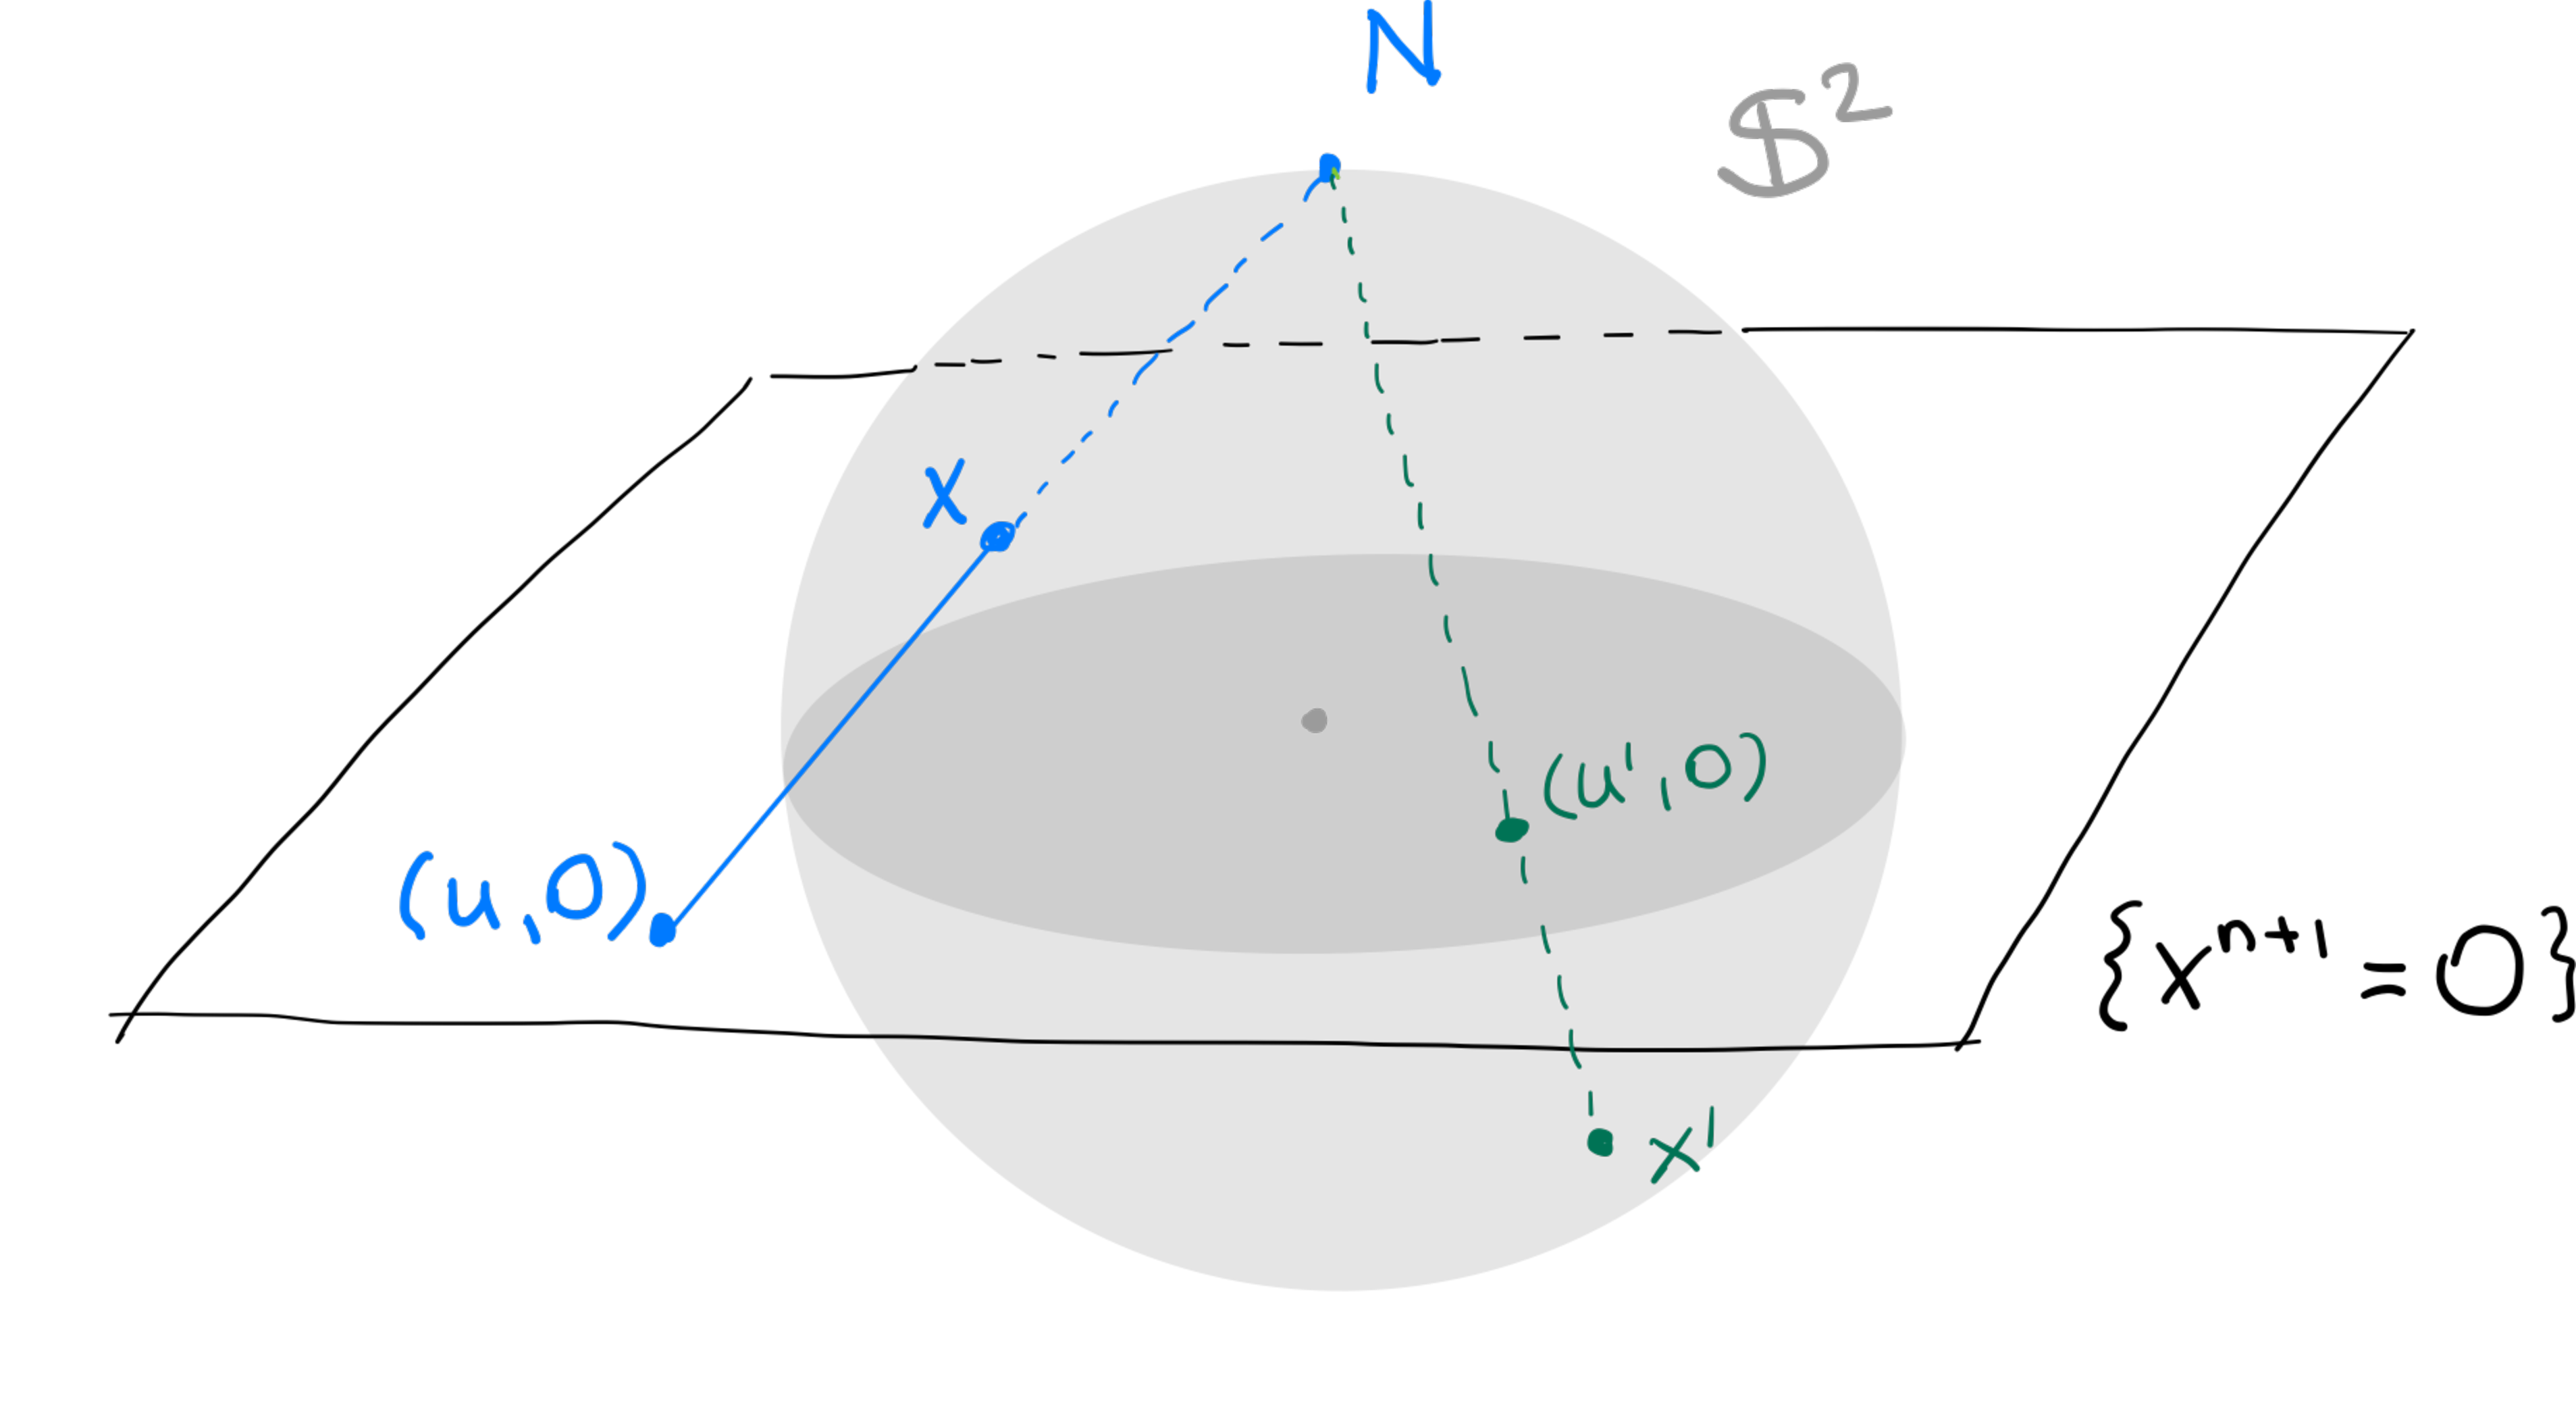
\includegraphics[trim=20pt 20pt 5pt 15pt,clip]{1_5_8-sphere}
  \end{marginfigure}
  \begin{equation}
    \sigma(x^1,\ldots,x^{n+1}) := \left(\frac{x^1}{1-x^{n+1}},\ldots,\frac{x^n}{1-x^{n+1}}\right),
  \end{equation}
  and $\widetilde\sigma:\bS^n\setminus\{S\}\to \R^n$, $\widetilde\sigma(x) := -\sigma(-x)$.
  \begin{enumerate}
    \item For any $x\in\bS^n\setminus\{N\}$, show that $\sigma(x)=u$ where $(u,0)$ is the point of intersection of the line passing through $N$ and $x$ with the hyperplane $\{x^{n+1}=0\}$.
      Similarly, show that $\widetilde\sigma(x)$ is the point where the line through $S$ and $x$ intersects the same hyperplane.
    \item Show that $\sigma$ is bijective and
      \begin{equation}
        \sigma^{-1}(u) = \left(\frac{2 u^1}{\|u\|^2+1}, \ldots,\frac{2 u^n}{\|u\|^2+1},\frac{\|u\|^2-1}{\|u\|^2+1}\right).
      \end{equation}
    \item Compute the transition map $\widetilde\sigma\circ\sigma^{-1}$ and verify that the atlas $\{(\bS^n\setminus\{N\},\sigma),(\bS^n\setminus\{S\},\widetilde\sigma)\}$ defines a smooth structure on $\bS^n$.
    \item Let $n=1$. Show that this smooth structure is the same as the one defined in Example~\ref{ex:S1emb}.
  \end{enumerate}
\end{exercise}

\begin{tcolorbox}
  The general definition of $C^r$-manifolds is mostly a matter of replacing occurrences of ``smooth'' in the text with $C^r$.
  The study of these more general structures is not dissimilar from what we will see in this course, with the exception of analytic and $C^0$-manifolds, but it introduces an unnecessary extra level of verbosity.
  In these notes we will only deal with smooth manifolds.
\end{tcolorbox}

\section{Smooth maps and differentiability}\label{sec:smoothfn}

With a well--defined differentiable structure and the idea of compatible charts, we have all the ingredients to lift the definition of differentiable maps from the euclidean world.

Before considering the general definition of a differentiable map, let's look at the simpler example of differentiable functions $f:M\to\R$ between a smooth manifold $M$ and $\R$.

\begin{marginfigure}
  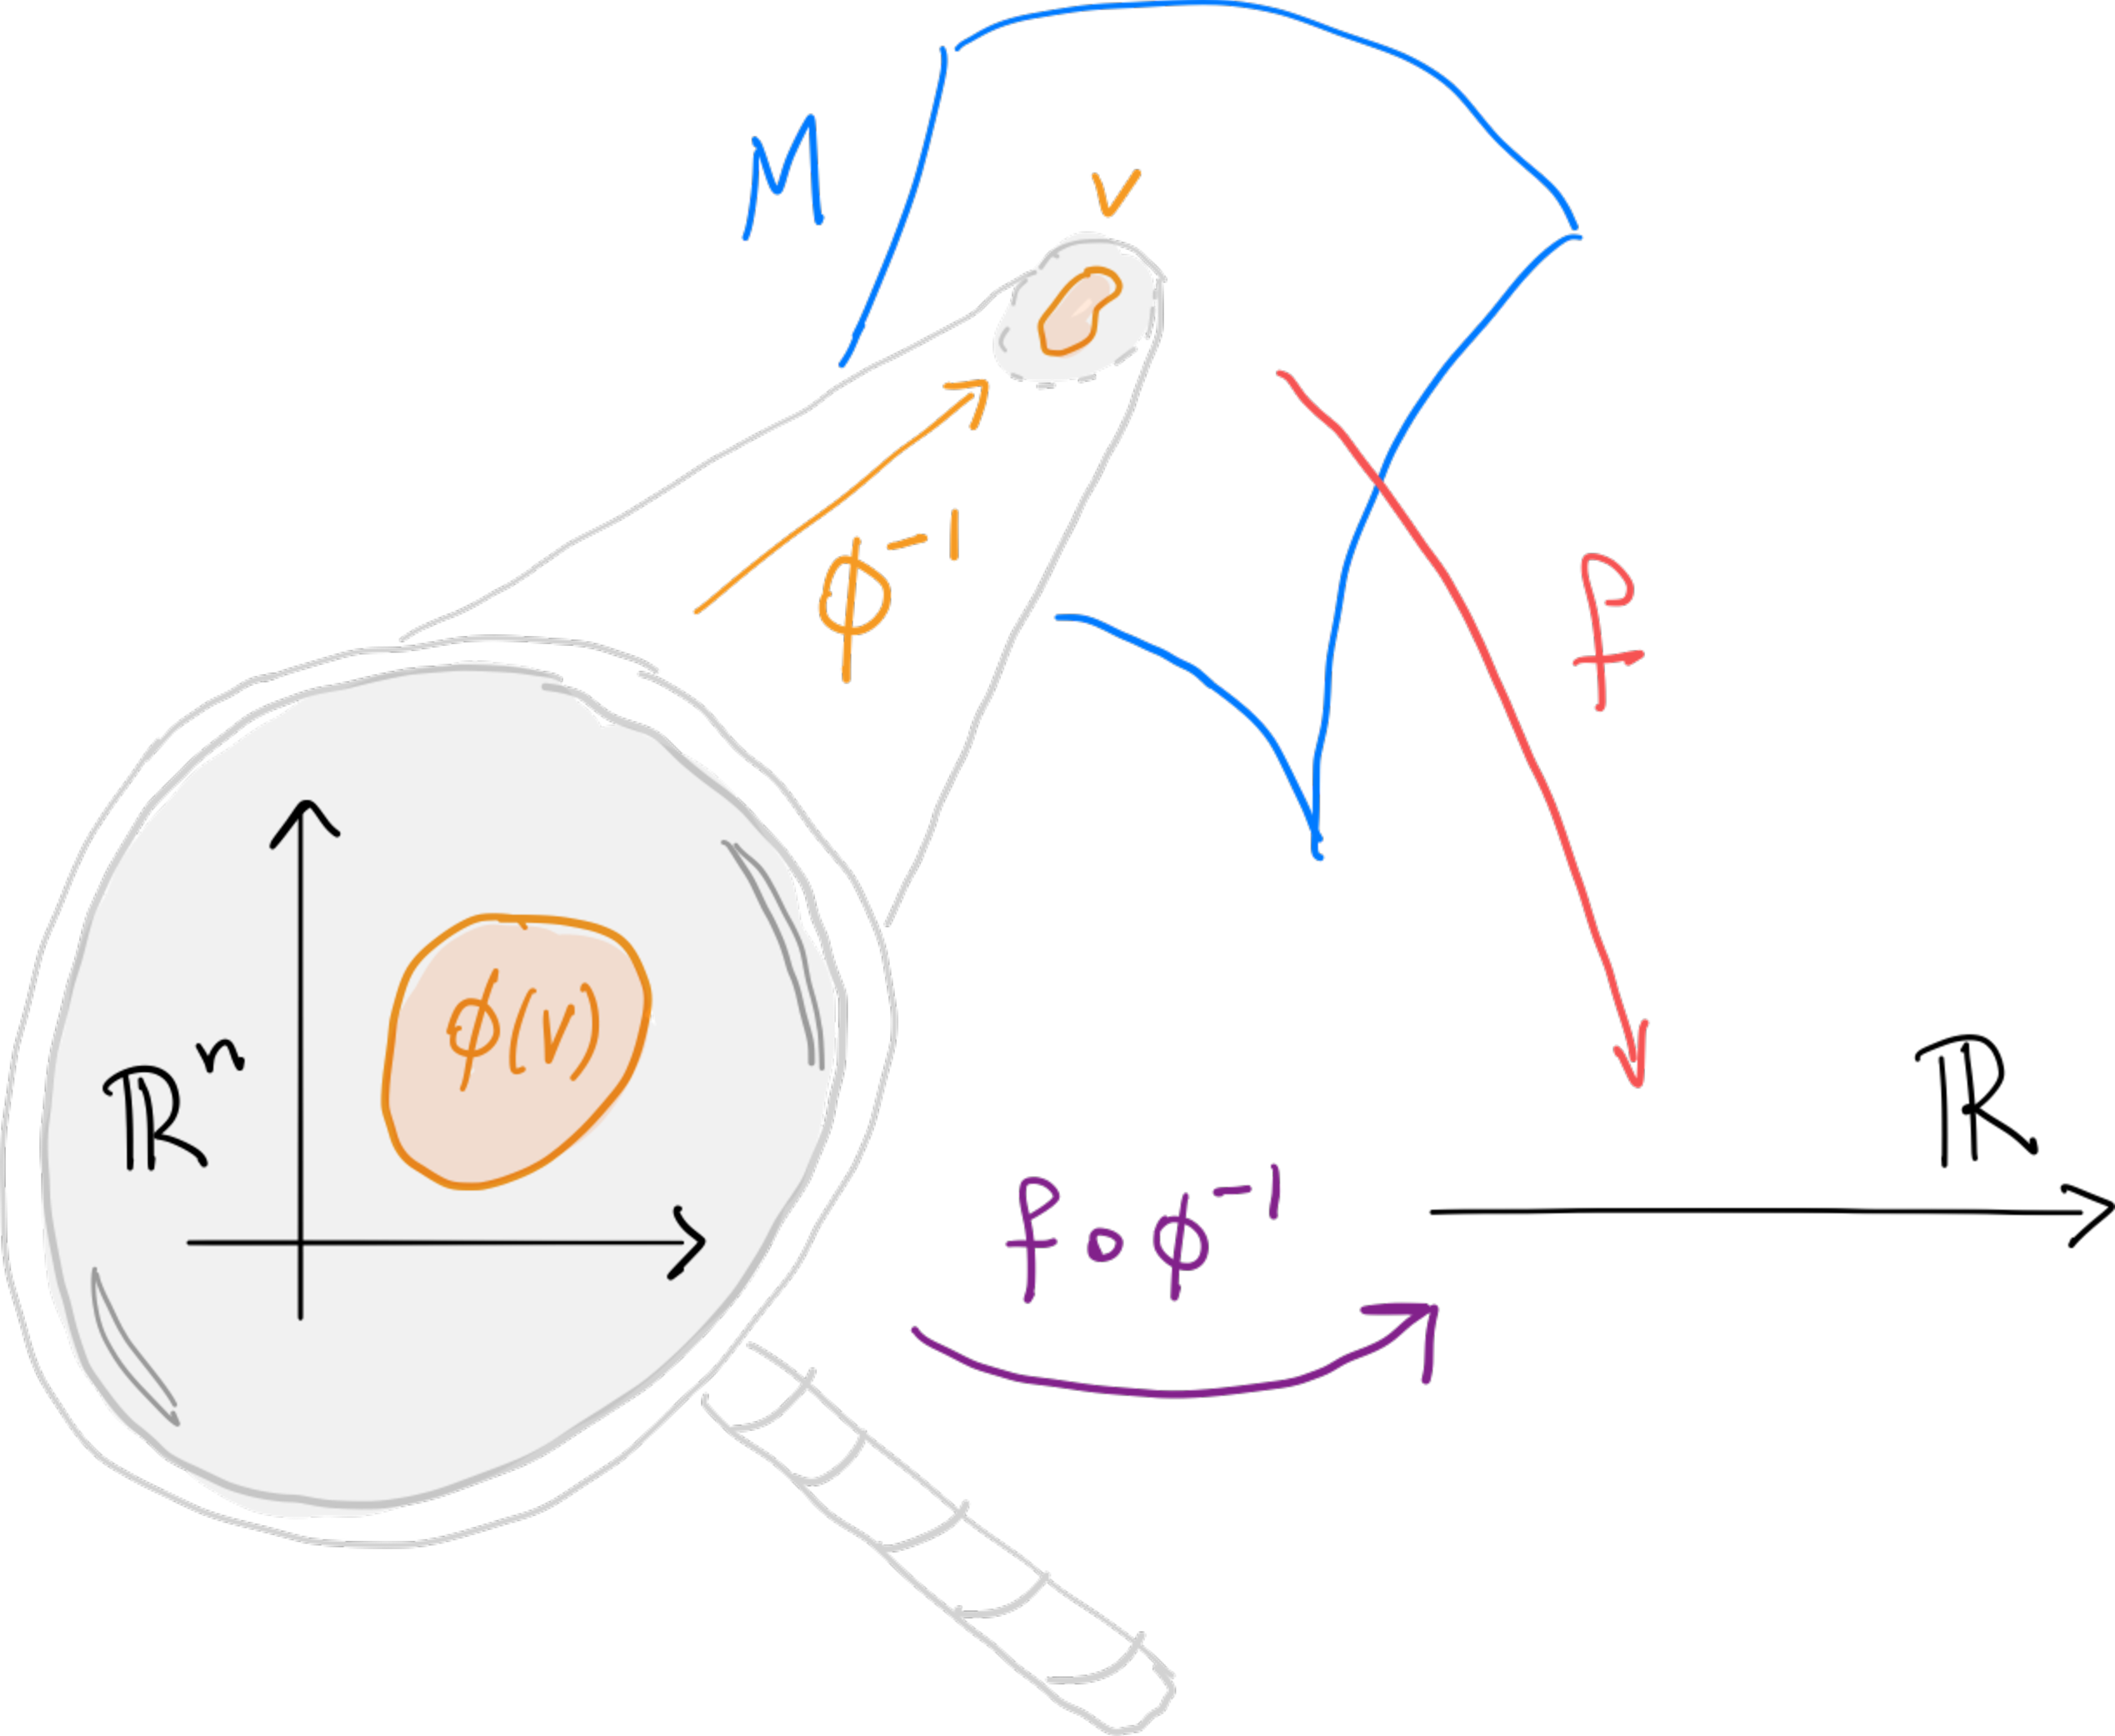
\includegraphics{1_5-diff-fun-v2.pdf}
  \label{fig:diff-fun}
  \caption{A function is differentiable if it is differentiable as a euclidean function through the magnifying lens provided by the charts.}
\end{marginfigure}
\begin{definition}
  A function $f:M\to\R$ from a smooth manifold $M$ of dimension $n$ to $\R$ is \emph{smooth}, or \emph{of class $C^\infty$}, if for any smooth chart $(\varphi, V)$ for $M$ the map $f\circ\varphi^{-1}:\varphi(V)\subset\R^n \to \R$ is smooth as a euclidean function on the open subset $\varphi(V)\subset\R^n$.
  We denote the space of smooth functions by $C^\infty(M)$.
\end{definition}

This, colloquially speaking, means that a function is differentiable if it is differentiable as a euclidean function through the magnifying lens (see Figure~\ref{fig:diff-fun}) provided by the charts.

\begin{exercise}
  Define the following operations on $C^\infty(M)$.
  For any $f,g\in C^\infty(M)$, $c\in\R$,
  \begin{equation}
    (f+g)(x) := f(x) + g(x),\quad
    (fg)(x) := f(x) g(x),\quad
    (cf)(x) := c f(x).
  \end{equation}
  Then, the space $C^\infty(M)$ endowed with the operations above is an \emph{algebra}\footnote{I.e. a vector space where you can also multiply two elements.} over $\R$.
\end{exercise}

The following theorem can be very convenient when you work with smooth functions.

\begin{proposition}
  Let $M$ be a smooth $n$-manifold and $f:M\to\R$ a real-valued function on $M$. Then, the following are equivalent:
  \begin{enumerate}[(i)]
    \item $f\in C^\infty(M)$;
    \item $M$ has an atlas $\cA$ such that for every chart $(U, \varphi)\in\cA$, $f\circ \varphi^{-1} : \R^n\supset\varphi(U)\to \R$ is $C^\infty$;
    \item for every point $p\in M$, there exists a smooth chart $(V,\psi)$ for $M$ such that $p\in V$ and the function $f\circ\psi^{-1} : \R^n\supset\psi(V)\to \R$ is $C^\infty$ on the open subset $\psi(V)\subset\R^n$.
  \end{enumerate}
\end{proposition}

\begin{exercise}
  Prove the proposition.\\
  \textit{\small Hint: go cyclic, for example show $(i)\Rightarrow(ii)$, $(ii)\Rightarrow(iii)$, $(iii)\Rightarrow(i)$.}
\end{exercise}

At this point, the generalization of smooth functions to smooth maps between manifolds should not come as a surprise.

\begin{definition}
  Let $F:M_1\to M_2$ be a continuous map \footnote{Remember: continuity is not a problem since $M_1$ and $M_2$ are topological spaces.} between two smooth manifolds of dimension $n_1$ and $n_2$ respectively.
  We say that $F$ is \emph{smooth}, or \emph{of class $C^\infty$}, if, for any chart $(\varphi_1, V_1)$ of $M_1$ and $(\varphi_2, V_2)$ of $M_2$, the map
  \begin{align}
    \varphi_2 \circ F \circ \varphi_1^{-1}: U_1 \to U_2,\qquad
    \begin{cases}
    U_1 := \varphi_1(V_1 \cap F^{-1}(V_2))\subset\R^{n_1}\\
    U_2 := \varphi_2(V_2)\subset\R^{n_2}
    \end{cases},
  \end{align}
  is smooth as a euclidean function.
  \marginnote[-6em]{Differently from your calculus classes, we are defining differentiability \emph{before} we define what the derivative is. Getting to it will require some amount of work, and will have to wait until the next chapter.}

  We denote by $C^\infty(M_1, M_2)$ the set of all functions $F:M_1\to M_2$ of class $C^\infty$.

  The map $\hat F := \varphi_2 \circ F \circ \varphi_1^{-1}$ is called the \emph{coordinate representation of $F$} with respect to the given coordinates.
\end{definition}

\begin{figure}[htp]
  \centering
  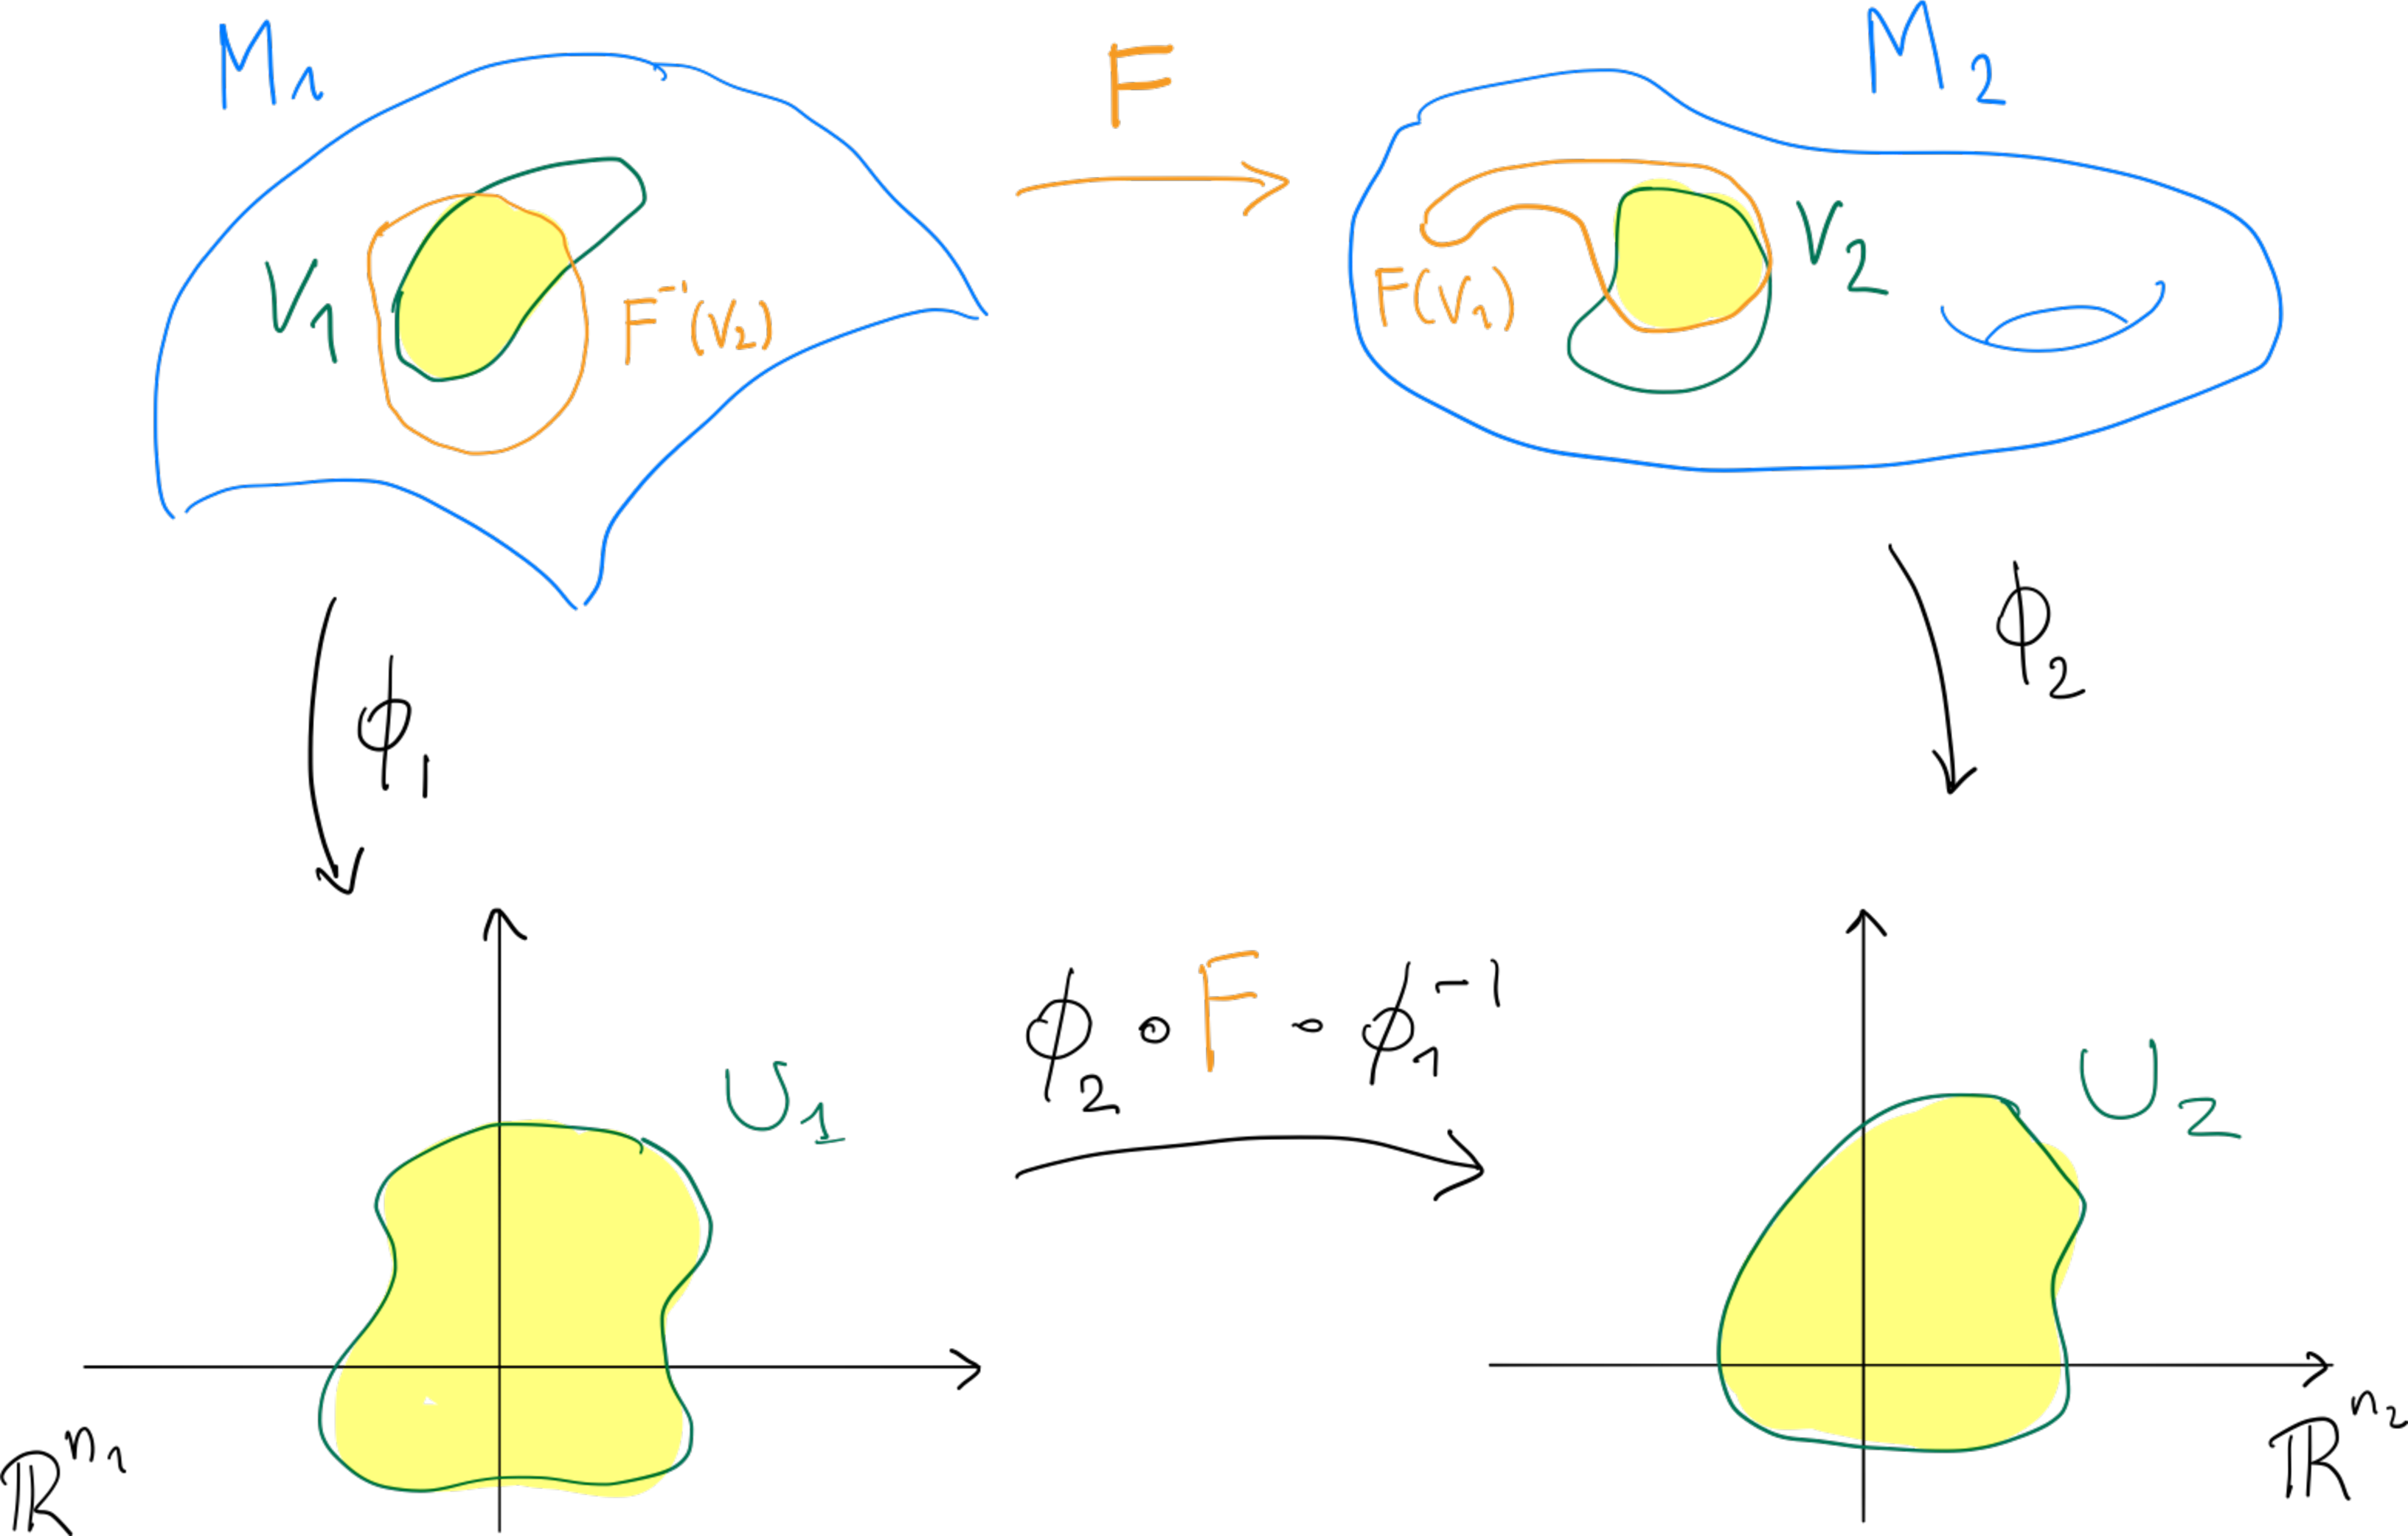
\includegraphics{1_3-diffble_maps.pdf}
  \caption{Maps are differentiable when they are differentiable as maps between euclidean spaces.}
  \label{fig:1.3-differentiable_maps}
\end{figure}

For a very simple and familiar example, consider the real valued function $f(x,y)= x^2+y^2$ defined on $\R^2$.
In polar coordinates on $U=\{(x,y)\in\R^2\mid x>0\}$, $f$ has the coordinate representation $\hat f (\rho, \theta) = \rho^2$.
Very often, where there is no ambiguity, we will simply identify $f$ and $\hat f$ and just write
\begin{quote}
  in the local coordinates $(\rho,\theta)$ on $U$, $f(\rho,\theta) = \rho^2$.
\end{quote}

A first observation about our definition of smooth maps is that, as one would hope, smoothness implies continuity.
%
\begin{exercise}
  Show that every smooth map is continuous.
\end{exercise}
%
\begin{exercise}
  Prove the following propositions, aiding your reasoning by drawing the relevant figures or commutative diagrams.
  \begin{proposition}
    Let $M$ be a smooth manifold of dimension $n$.
    Then $F:M\to\R^m$ is smooth iff for all smooth charts $(U,\varphi)$ of $M$, the function $F\circ\varphi^{-1}:\varphi(U)\to\R^m$ is smooth.
  \end{proposition}
  \begin{proposition}
    Let $M$ be a smooth manifold of dimension $n$.
    Then $F:\R^m\to M$ is smooth iff for all smooth charts $(U,\varphi)$ of $M$, the function $\varphi\circ F:F^{-1}(U)\to\R^n$ is smooth.
  \end{proposition}
  \begin{proposition}
    Let $M, N, P$ be three smooth manifolds, and suppose that $F:M\to N$ and $G:N\to P$ are smooth.
    Then $G\circ F\in C^\infty(M, P)$.
  \end{proposition}

  \begin{proposition}[Smoothness is a local property]\label{prop:smoothlocal}
    Let $F:M\to N$ be a continuous function and let $\{U_i\}_{i\in I}$ be an open cover for $M$. Then $F|_{U_i}:U_i \to N$ is smooth for every $i\in I$ iff $F:M\to N$ is smooth.
  \end{proposition}
\end{exercise}

It can be useful to know that there are alternative ways to characterize smooth functions.
\begin{exercise}[Equivalent definitions of smoothness]\label{prop:eq-def-smooth}
  Let $M_1$ and $M_2$ be smooth manifolds.
  Show that a map $F:M_1\to M_2$ is smooth if and only if either of the following conditions holds:
  \begin{enumerate}
    \item for every $p\in M_1$, there are smooth charts $(V_1,\phi_1)$, $p\in V_1$, and $(V_2,\phi_1)$, $F(p) \in V_2$, such that $F(V_1) \subseteq V_2$ and $\phi_2 \circ F \circ \phi_1^{-1}$ is smooth from $\phi_1(V_1)$ to $\phi_2(V_2)$;
    \item $F$ is continuous and there exists two smooth atlases $\{(V^1_\alpha, \phi^1_\alpha)\}$ and $\{(V^2_\beta, \phi^2_\beta)\}$, respectively for $M_1$ and $M_2$, such that for each $\alpha$ and $\beta$, $\phi^2_\beta \circ F \circ (\phi^1_\alpha)^{-1}$ is a smooth maph from $\phi^1_\alpha(V^1_\alpha \cap F(V_\beta^2))$ to $\phi^2_\beta(V^2_\beta)$.
  \end{enumerate}
\end{exercise}

\begin{definition}
  A \emph{diffeomorphism} $F$ between two smooth manifolds $M_1$ and $M_2$ is a bijective map such that $F\in C^\infty(M_1, M_2)$ and $F^{-1}\in C^\infty(M_2, M_1)$.
  %
  Two smooth manifolds $M_1$ and $M_2$ are called \emph{diffeomorphic} if there exists a diffeomorphism $F:M_1\to M_2$ between them.
\end{definition}

\begin{exercise}
  Any chart $(V, \varphi)$ of a manifold $M$ is a diffeomorphism between the manifolds $V\subset M$ and $\varphi(V)\subset\R^n$.
\end{exercise}

\begin{exercise}
  Prove that $\R^2\setminus\{(0,0)\}$ is a two-dimensional manifold and construct a diffeomorphism from this manifold to the circular cylinder
  \begin{equation}
    C := \{ (x,y,z)\in\R^3 \mid x^2+y^2 = 1\}\subset\R^3.
  \end{equation}
\end{exercise}

The following corollary is just a restatement of Proposition~\ref{prop:smoothlocal}, but provides a useful perspective on the construction of smooth maps.

\begin{proposition}[Gluing lemma for smooth maps]
  Let $M$ and $N$ be two smooth manifolds and let $\{U_\alpha\mid\alpha\in A\}$ be an open cover of $M$.
  Suppose that for each $\alpha\in A$ we are given a smooth map $F_
  \alpha:U_\alpha\to N$ such that the maps agree on the overlaps: $F_\alpha|_{U_\alpha\cap U_\beta} = F_\beta|_{U_\alpha\cap U_\beta}$ for all $\alpha,\beta\in A$. 
  Then there exists a unique smooth map $F:M\to N$ such that $F|_{U_\alpha} = F_\alpha$ for each $\alpha\in A$.
\end{proposition}

In other words, if you can define a map in a neighbourhood of each point in such a way that the locally defined maps all agree where they overlap, then the local definitions piece together to yield a global smooth map.
We will use this construction repeatedly throughout the course.
Sometimes, however, the local definitions are not guaranteed to agree. In this case one usually has to resort to a different tool: partitions of unity.
These allow to surgically patch objects together and make sure that they still have the required properties.
In the next section we will look more deeply into this.

\begin{tcolorbox}
  From now on, when we write manifold, chart, atlas, etc. we always mean smooth manifold, smooth chart, smooth atlas, etc..
\end{tcolorbox}

\begin{example}[A different smooth structure on $\R$]
  Consider the homeomorphism $\psi:\R\to\R$, $\psi(x) = x^3$.
  The atlas consisting of the global chart $(\R, \psi)$ defines a smooth structure on $\R$.
  This chart is not smoothly compatible with the standard smooth structure on $\R$ since $\id_\R \circ \psi^{-1} (y) = y^{1/3}$ is not smooth at $y=0$.
  Therefore, the smooth structure defined on $\R$ by $\psi$ is different from the standard one.
  You can adapt this idea to construct many different smooth structures on topological manifolds provided that they at least have one smooth structure.
\end{example}

\begin{exercise}
  Show that the smooth manifolds $(\R, \{(\R, \id_\R)\})$ and $(\R, \{(\R, \psi)\})$, defined using the smooth structures from the previous example, are diffeomorphic.
\end{exercise}

\begin{exercise}
  For $r>0$, let $\phi_r:\R\to\R$ be the map given by
  \begin{equation}
    \phi_r(t) := \begin{cases}
      t, & \mbox{if } t<0,\\
      rt, & \mbox{if } t\geq0.
    \end{cases}
  \end{equation}
  Let $\cA_r$ denote the maximal atlas on $\R$ containing the chart $(\R, \phi_r)$.
  \begin{enumerate}
    \item Show that the differentiable structures on $\R$ defined by $\cA_r$ and $\cA_s$, $0<r<s$, are different.
      This shows that there are uncountably many families of different differential structures on $\R$.
    \item Let $M_r$ be the manifold $\R$ equipped with the atlas $\cA_r$.
      Show that $M_r$ and $M_s$ are diffeomorphic for $r,s >0$.
  \end{enumerate}
\end{exercise}

\begin{remark}
  There exist examples of topological manifolds without smooth structures.
  It is also known that smooth manifolds of dimension $n < 4$ have exactly one smooth structure (up to diffeomorphisms) while ones of dimension $n > 4$ have finitely many\footnote{A beautiful example of this is the $7$-sphere $\bS^7$ which is known to have 28 non-diffeomorphic smooth structures.}.
  The case $n = 4$ is unknown: if you prove that there is only one smooth structure, you will have shown the smooth Poincar\'e conjecture.
\end{remark}

As a final exercise, we are going to relate smoothness of the maps with the smoothness of their components, which can be extremely useful when working in coordinates.

\begin{exercise}
  Let $F: M^m \to N^n$ be a continuous map between two manifolds. Then the following are equivalent:
  \marginnote{Recall Notation~\ref{ntn:coords}}
  \begin{enumerate}
    \item $F$ is smooth;
    \item $N$ has an atlas $\cA$ such that for all the charts $(V, \psi) = (V, y^1, \ldots, y^n)\in \cA$, the components $y^i \circ F: F^{-1}(V) \to \R$ of $F$ relative to the chart are all smooth;
    \item for every chat $(V, \psi) = (V, y^1, \ldots, y^n)$ on $N$, the components $y^i \circ F: F^{-1}(V) \to \R$ of $F$ relative to the chart are all smooth.
  \end{enumerate}
  Note that this, in particular, holds for $N=\R^n$.
\end{exercise}

\section{Partitions of unity}

\newthought{Cutoff functions} are a class of smooth functions that will be of crucial importance throughout the course, and whose existence cannot be given for granted.
Since their definition and construction does not require more than what we have just seen, let's talk about them now.

First of all, recall that the \emph{support} of a smooth function $f: M \to \R$, denoted by $\supp(f)$, is defined as
\marginnote[2em]{The bar over the set denotes its closure.}
\begin{equation}
  \supp(f) := \overline{\{ p\in M \;\mid\; f(p) \neq 0\}}.
\end{equation}

We will introduce those functions with a proposition, and will spend the rest of this chapter proving it.

\begin{figure}[htp!]
  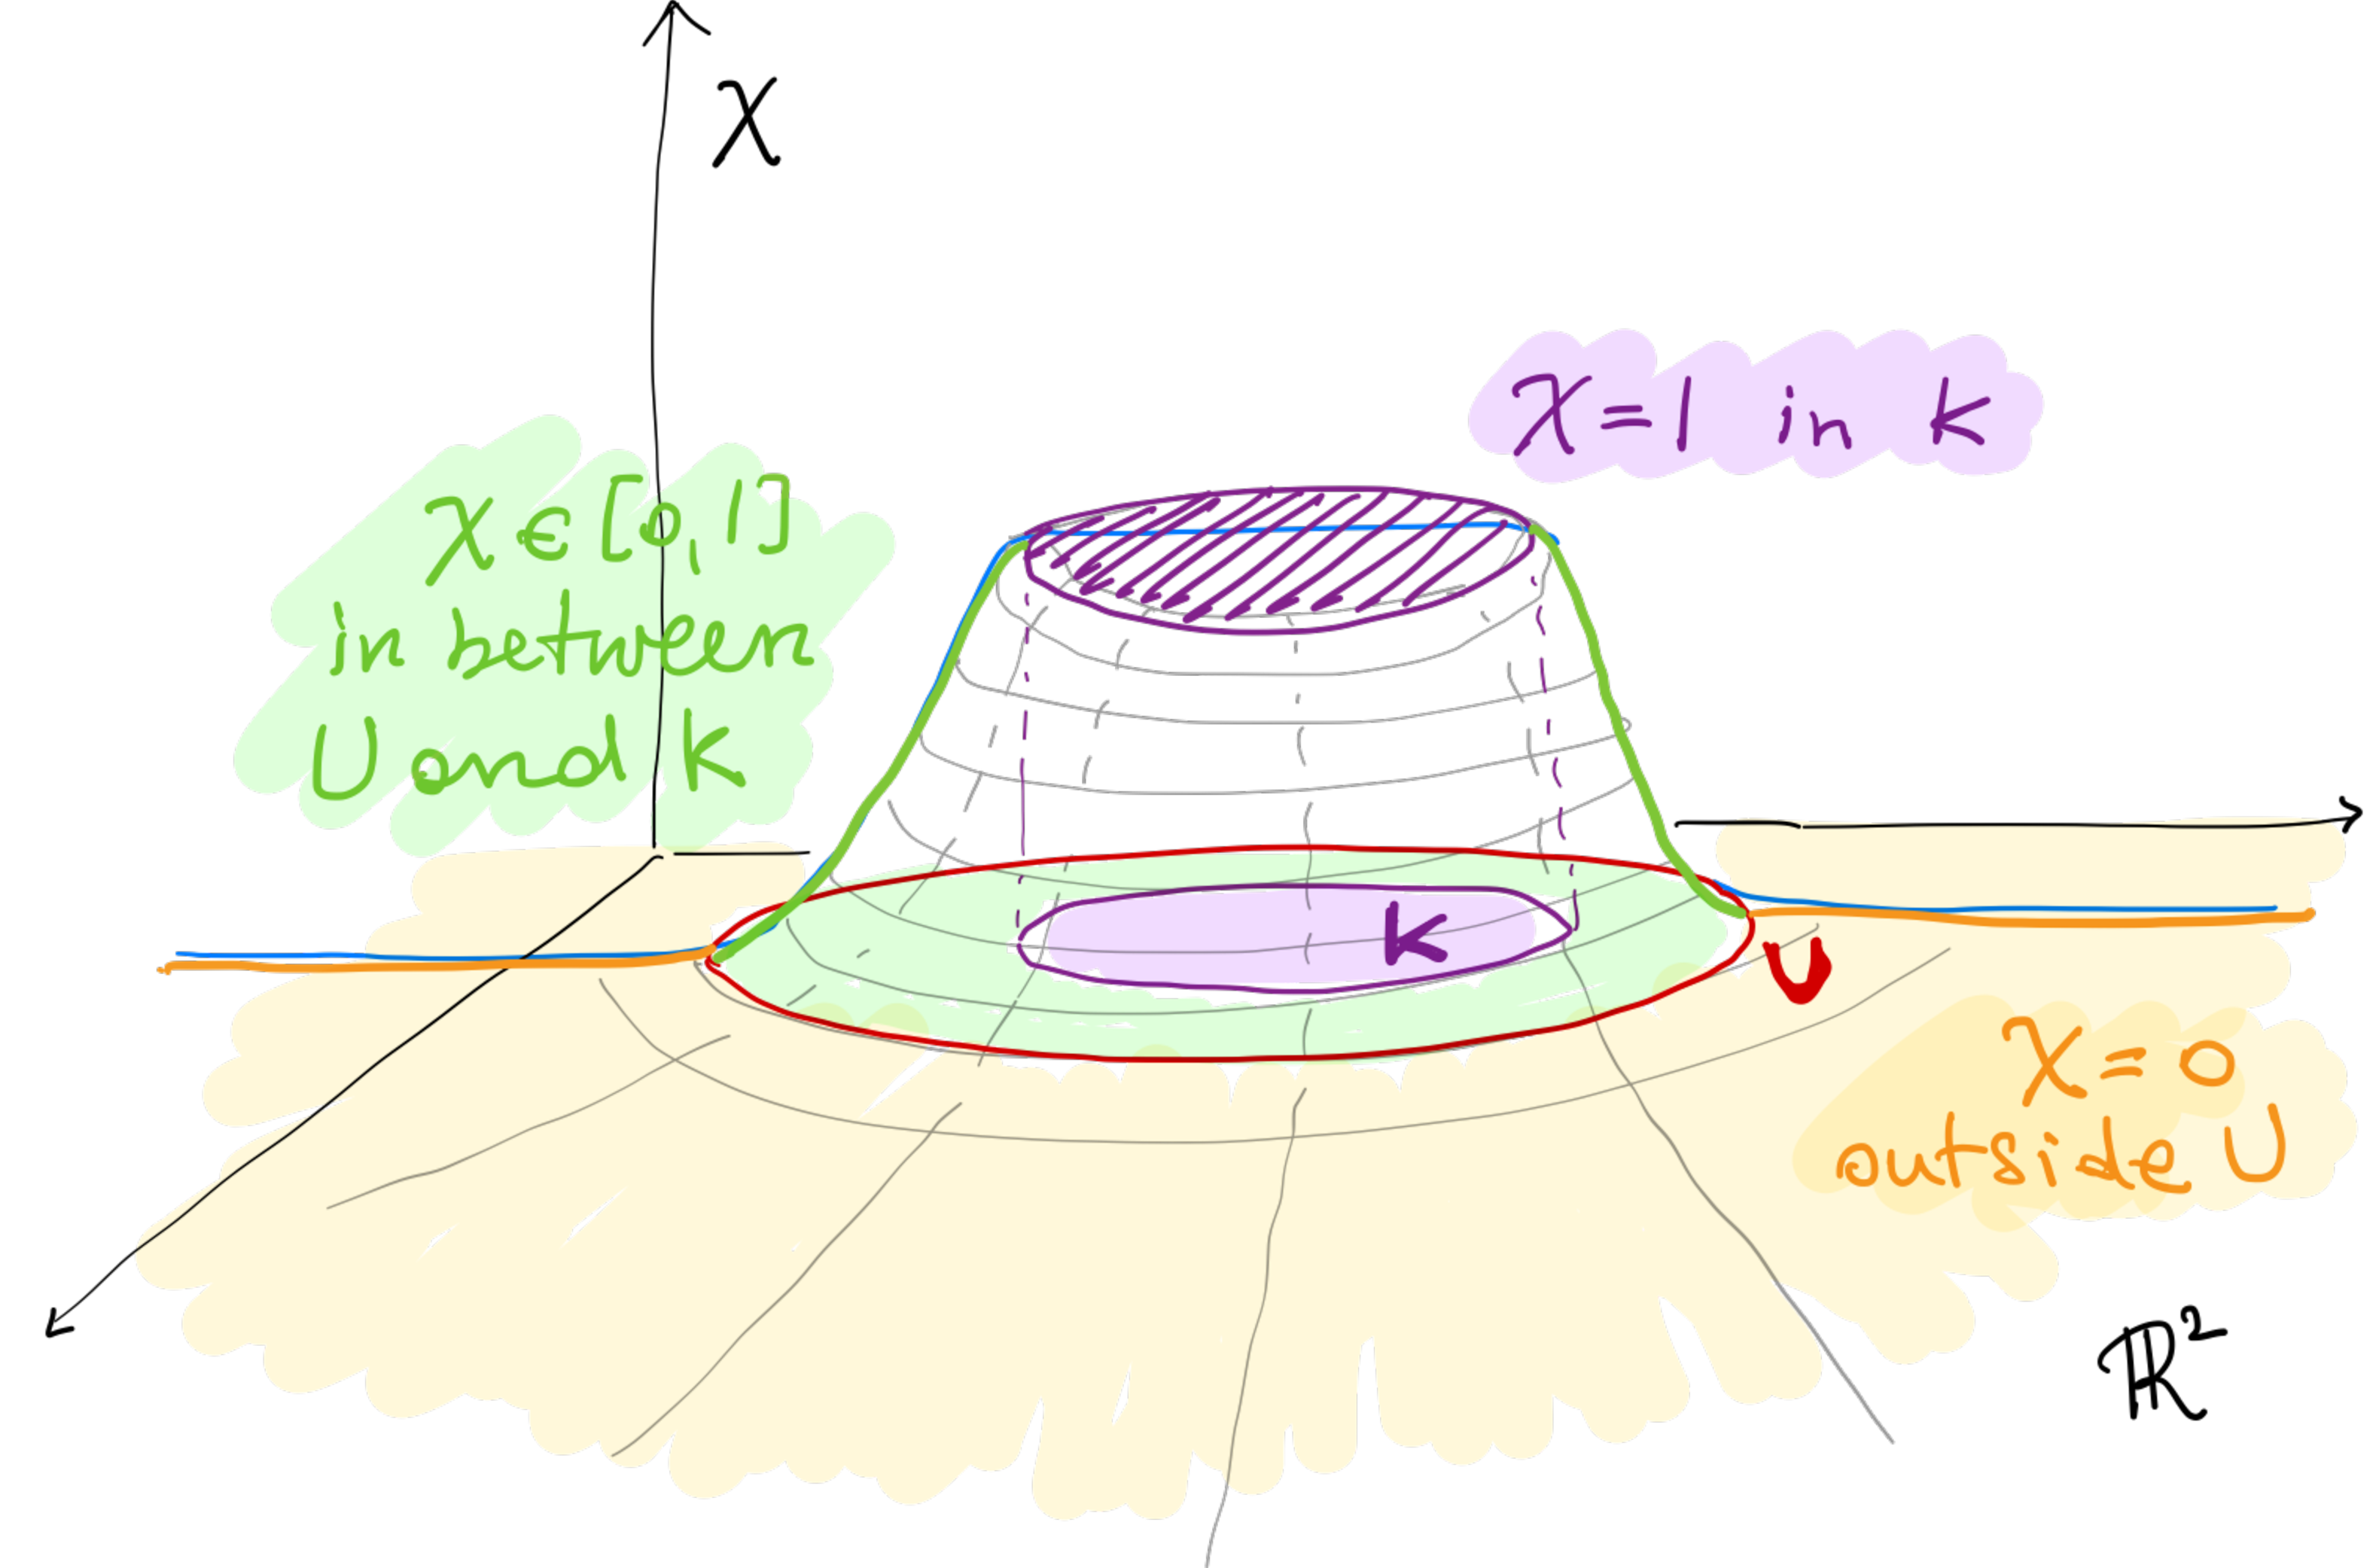
\includegraphics{1_6-cutoffs.pdf}
\end{figure}

\begin{proposition}[Cutoff functions]\label{prop:cutoff}
  Let $M$ be a smooth manifold and $K\subset U\subset M$ two subsets such that $K$ is closed and $U$ is open.
  Then, there exists a smooth function $\chi: M \to\R$, called \emph{cutoff} function, with the following properties
  \begin{enumerate}[(i)]
    \item $0 \leq \chi \leq 1$ for all $p\in M$;
    \item $\supp(\chi)\subset U$;
    \item $\chi(p) = 1$ for all $p\in K$.
  \end{enumerate}
\end{proposition}

The proof of this proposition involves a general result which is quite technical and whose proof will be omitted.
You can refer to~\cite{book:lee, book:tu} if you are curious to see the details.

Instead, we will show a special case of Proposition~\ref{prop:cutoff}. The main reason is that it involves an explicit construction of the cutoff which can be convenient to have at hand later on.

\begin{lemma}[Cutoff functions, compact case]
  Let $M$ be a smooth manifold and $K\subset U\subset M$ two subsets such that $K$ is compact and $U$ is open.
  Then, there exists a smooth function $\chi: M \to\R$ with the following properties
  \begin{enumerate}[(i)]
    \item $0 \leq \chi \leq 1$ for all $p\in M$;
    \item $\supp(\chi)\subset U$;
    \item $\chi(p) = 1$ for all $p\in K$.
  \end{enumerate}
\end{lemma}
\begin{proof}
  \newthought{Part 1}.
  To warm up, let's do some first year analysis.
  For any pair of real numbers $r < R$ there exists a smooth function $f: \R \to [0,1]$ such that $f(t) = 1$ for $t \leq r$, $f(t) = 0$ for $t \geq R$ and $0<f(t)<1$ for $t\in(r,R)$.

  We can construct this explicitly by means of the function
  \begin{equation}
    h:\R\to\R, \quad h(t):= \begin{cases}
      e^{-1/t}, & t>0,\\
      0, & t \leq 0.
    \end{cases}
  \end{equation}

  \begin{exercise}
    Prove by induction that for $t>0$ and $k\geq 0$, the $k$th derivative $h^{(k)}(t)$ is of the form $p_{2k}(1/t)e^{-1/t}$ for some polynomial $p_{2k}(x)$ of degree $2k$ in $x$.
    Use this to show that $h\in C^\infty(\R)$ and that $h^{(k)}(0) = 0$ for all $k\geq 0$.
  \end{exercise}

  The function $f$ that we are seeking is then\footnote{Exercise: check that such function $f$ satisfies all the desired properties.} given by
  \begin{equation}
    f(t) := \frac{h(R-t)}{h(R-t) + h(t-r)}.
  \end{equation}

  \newthought{Part 2}.
  Let's extend $f$ to $\R^n$.
  Denote $B_r \subset \R^n$ the open ball of radius $r$ around the origin.
  Then, for any $0 < r < R$ we seek a function $g:\R^n\to\R$ such that $g(x) = 1$ for all $x\in \overline{B_r}$, $g(x) = 0$ for all $x\in \R^n\setminus B_R$ and $0< g(x)< 1$ for all $x\in B_R\setminus\overline{B_r}$.
  This is immediately achieved by defining $g(x) := f(\|x\|)$, where $f$ is the function defined in the previous step.

  \newthought{Part 3}.
  Let's now pick a point $p\in M$ and an arbitrary neighbourhood $U$ of $p$. Choosing an appropriate chart about $p$, the previous step implies that we can choose a smaller neighbourhood $V\subset U$ of $p$ with $\overline V\subset U$ and such that there exists a smooth function $\chi: M \to [0,1]$ satisfying $\chi(p) = 1$ for all $p\in\overline{V}$ and $\chi(p) = 0$ for all $p\in M\setminus U$.

  \newthought{Part 4}.
  We are ready to complete the proof.
  For each point $p\in K$, choose two neighbourhoods $V_p \subset U_p$ such that $\overline{V_p}\subset K$ and $U_p \subset U$.
  Since $K$ is compact, it admits a finite cover in terms of these sets: i.e. there are finitely many points $p_1, \ldots, p_N \in K$ such that $K \subset \bigcup_{i=1}^N V_{p_i}$.
  For each $i$, choose $\chi_i: M \to [0,1]$ as in the previous step: $\chi_i(p) = 1$ for all $p\in\overline{V_{p_i}}$ and $\chi_i(p) = 0$ for all $p\in M\setminus U_{p_i}$.
  The proof is completed by defining
  \begin{equation}
    \chi := 1 - \prod_{i=1}^N(1 - \chi_i(p)).
  \end{equation}
\end{proof}

We are not there yet. To extend this result to our needs will need a new tool, which will be useful throughout the course and in many courses to come.

\begin{definition}
  Let $M$ be a smooth manifold. A \emph{partition of unity} is a collection $\{\rho_\alpha \mid \alpha\in A\}$ of functions $\rho_\alpha:M\to\R$ such that
  \begin{enumerate}[(i)]
    \item $0 \leq \rho_\alpha \leq 1$ for all $p\in M$ and $\alpha\in A$;
    \item\label{def:pou.2} the collection $\{\rho_\alpha \mid \alpha\in A\}$ is \emph{locally finite}, that is, for any $p\in M$ there are at most finitely many $\alpha\in A$ such that $p\in\supp(\rho_\alpha)$;
    \item for all $p\in M$ one has $\sum_{\alpha\in A} \rho_\alpha(p) = 1$.
      \marginnote{For any $p$, $\sum_{\alpha\in A} \rho_\alpha(p)$ is a finite sum by~\ref{def:pou.2}. Thus, the function defined by the sum $\rho := \sum \rho_\alpha$ is a well define smooth function on $M$. We call such sum a \emph{locally finite} sum.}
  \end{enumerate}
\end{definition}

\begin{remark}
  Note that the existence of a partition of unity is a distinguished feature of differentiable manifolds: stronger structures, like analytic or holomorphic ones, in general fail to have one.
\end{remark}

Throughout the course we will be mostly interested in partitions of unity $\{\rho_\alpha \mid \alpha\in A\}$ which are \emph{subordinate} to an open cover $\{U_\alpha\mid\alpha\in A\}$, that is, such that $\supp_\alpha(\rho_\alpha) \subset U_\alpha$ for each $\alpha\in A$.

\begin{theorem}\label{thm:partitionof1}
  \marginnote[1.5em]{We are going to omit the proof of this theorem, for its details you can refer to~\cite[Proposition 13.6]{book:tu} or~\cite[Theorem 2.23]{book:lee}.}
  Let $M$ be a smooth manifold. For any open cover $\{U_\alpha\mid\alpha\in A\}$ of $M$, there exists a partition of unity $\{\rho_\alpha \mid \alpha\in A\}$ subordinate to $\{U_\alpha\mid\alpha\in A\}$.
\end{theorem}

With this result at hand, Proposition~\ref{prop:cutoff} can be shown very easily.

\begin{proof}[Proof of Proposition~\ref{prop:cutoff}.]
  Consider the open cover of $M$ given by $\cC:=\{M\setminus K, U\}$.
  Then Theorem~\ref{thm:partitionof1} implies that there exists a partition of unity $\{\rho_U, \rho_{M\setminus K}\}$ adapted to $\cC$. The function $\chi := \rho_U$ is our cutoff function.
\end{proof}

\section{Manifolds with boundary}\label{sec:mbnd}

\newthought{The definition of manifolds has a serious limitation}, even though it is perfectly good to describe curves\footnote{E.g. the circle seen in Example~\ref{ex:S1emb}.} and surfaces\footnote{E.g. the $2$-spheres $\bS^2$.}, it fails to describe many natural objects like a \emph{closed} interval $[a,b]\in\R$ or the \emph{closed} disk $D_1(0)$ of Example~\ref{ex:uball}.
Note that in each of these cases, both the interior and the boundary are smooth manifolds and their dimension differ by one\footnote{In the first case the interior $(a,b)$ is a $1$-manifold and the boundary, the set $\partial[a,b] = \{a,b\}$, is a $0$-manifold. In the second case the interior of $D_1(0)$ is the open unit ball, a $2$-manifold, and the boundary $\partial D_1(0)$ is the $1$-manifold $\bS^1$.}.

Let's do a step back and think about topological manifolds: since both the closed interval and the closed disk are closed sets, we have problems to make them locally euclidean in neighbourhoods of their boundaries.
Can we modify our local model to resemble something with a boundary?

Of course this is a rhetorical question.
We can generalize our definition by considering the \emph{closed upper half-spaces}
\begin{marginfigure}[2em]
  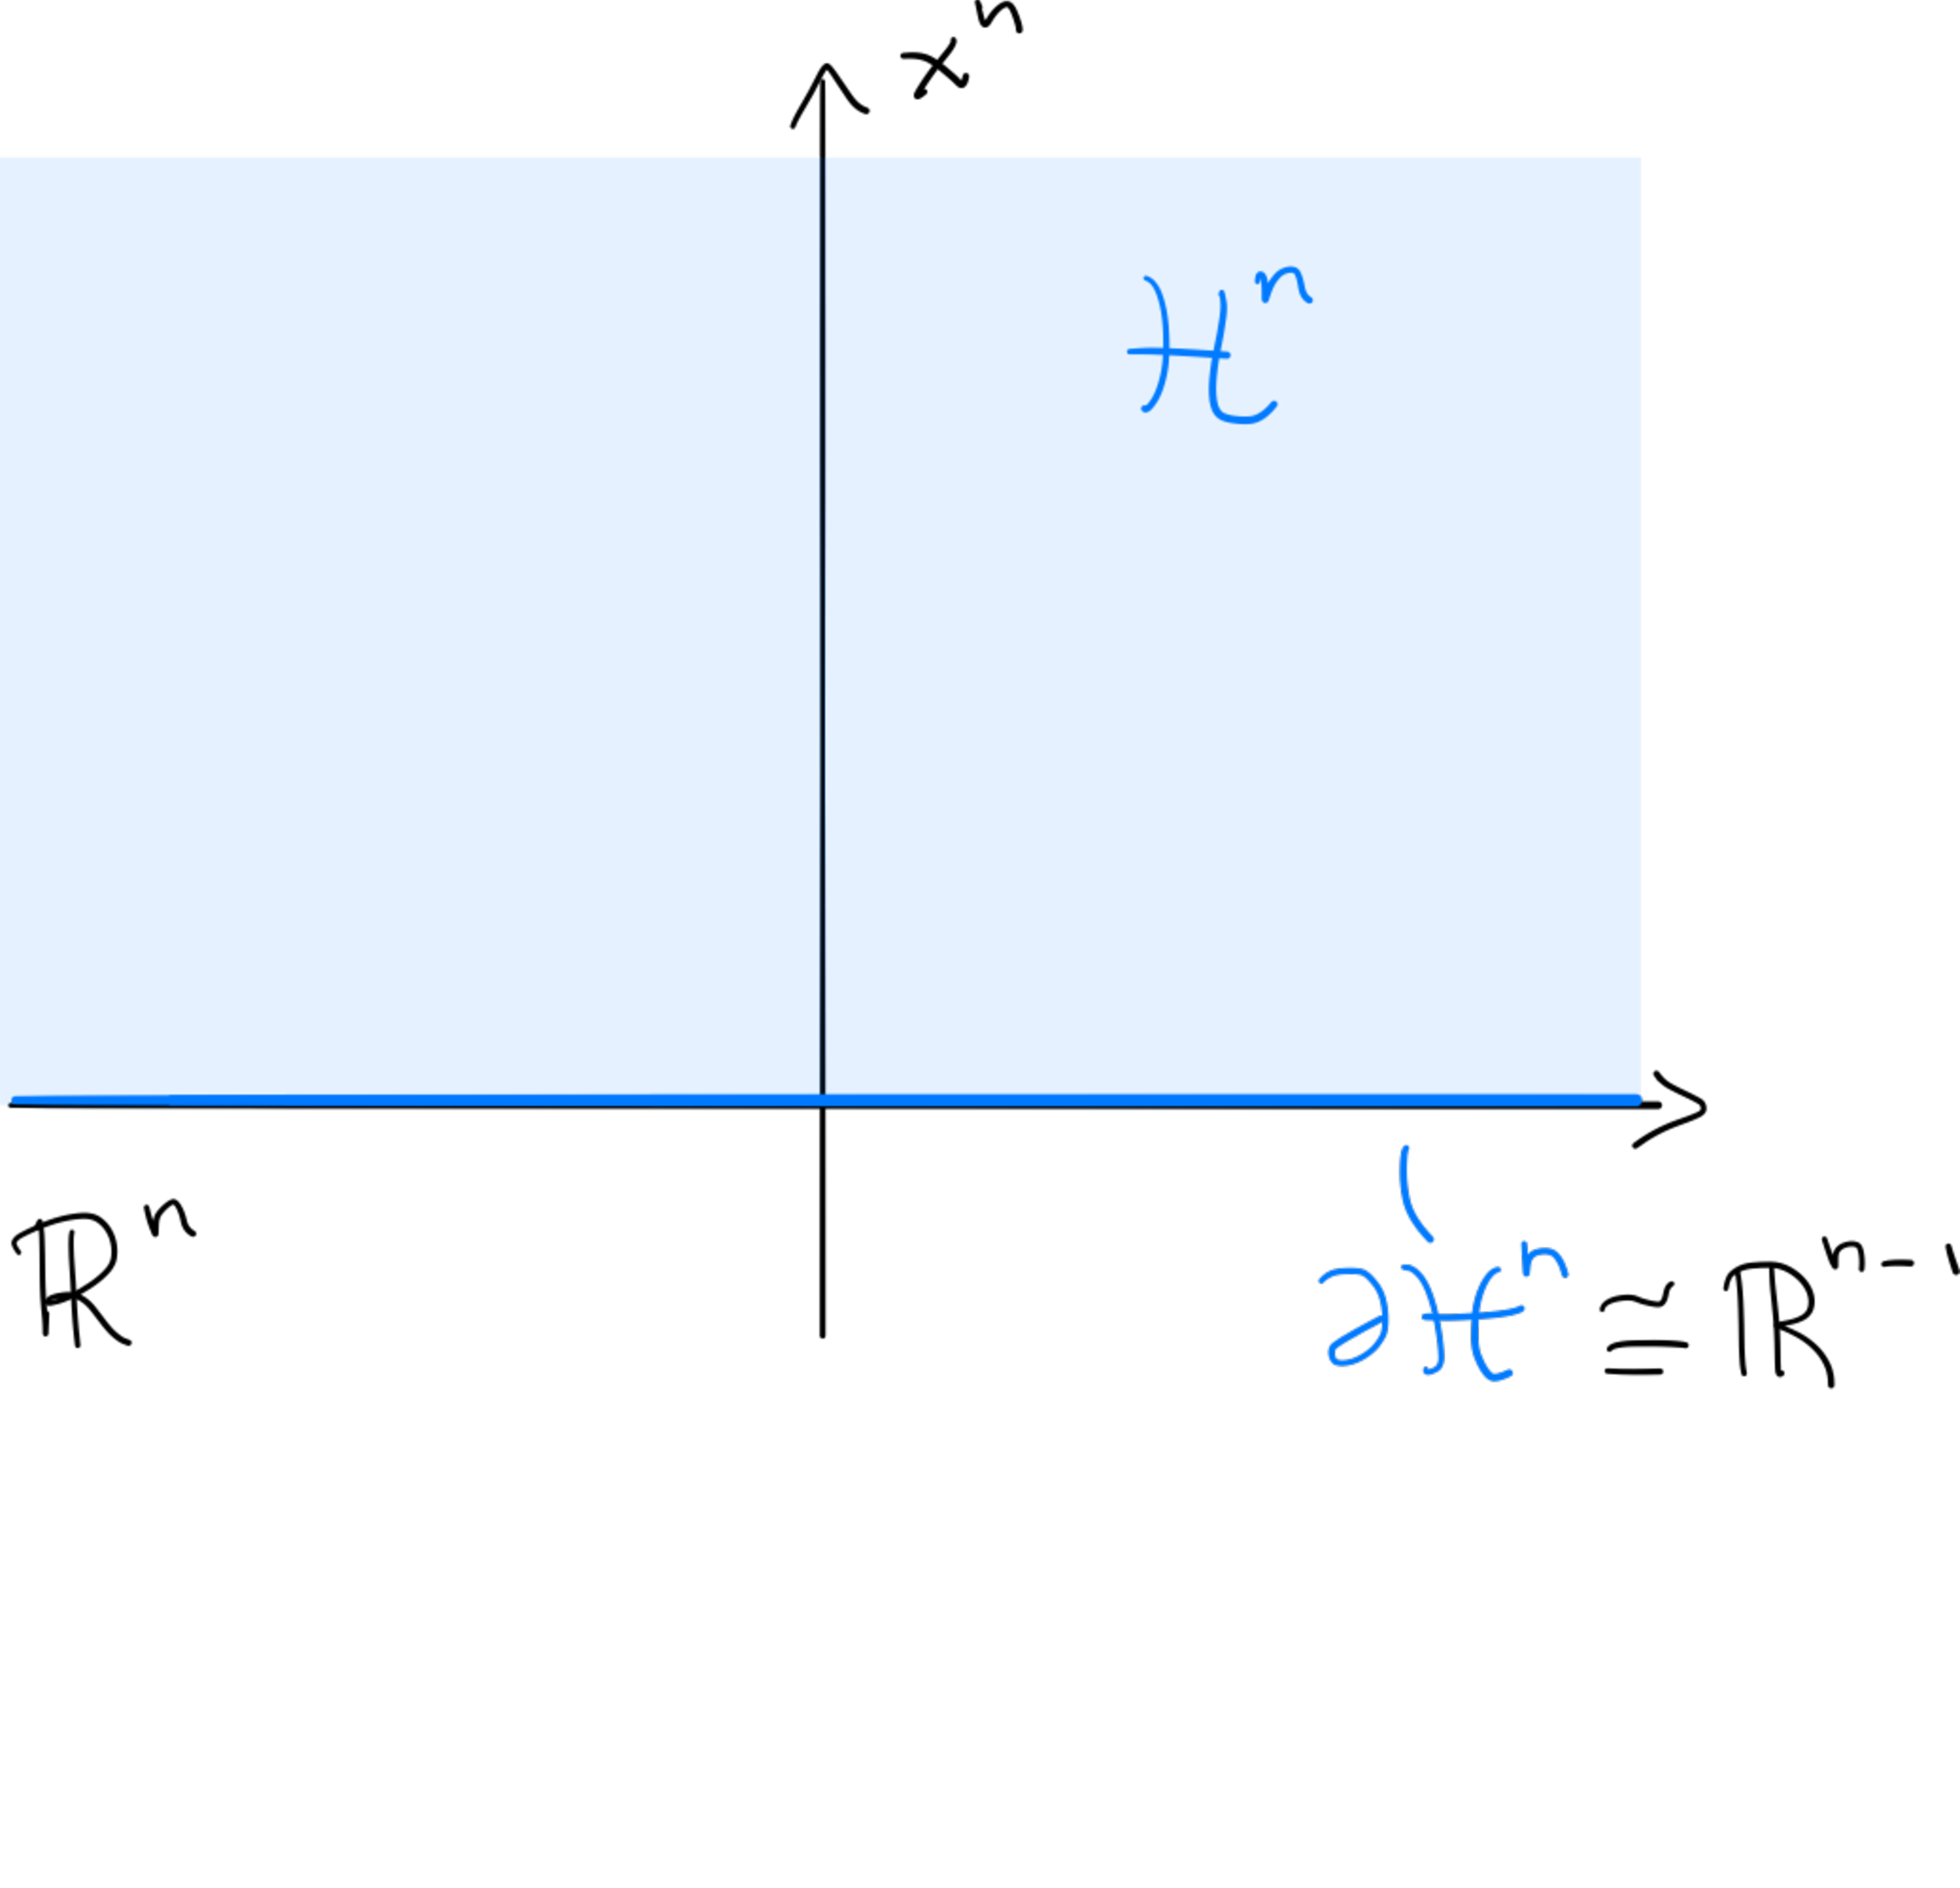
\includegraphics{1_4-upper_space.pdf}
\end{marginfigure}
\begin{equation}
  \cH^n = \{x=(x^1, \ldots, x^n)\in\R^n\mid x^n \geq 0\},
\end{equation}
with its $(n-1)$-dimensional boundary
\begin{equation}
  \partial\cH^n = \{x=(x^1, \ldots, x^n)\in\R^n\mid x^n = 0\}
\end{equation}
and the topology inherited by $\R^n$, as a replacement for our local model $\R^n$.

\begin{definition}
  A topological space $M$ is a \emph{topological manifold with boundary} of dimension $n$, or topological $n$-manifold with boundary, if it has the following properties
  \begin{enumerate}[(i)]
    \item $M$ is a Hausdorff space;
    \item $M$ is second countable;
    \item $M$ is \emph{locally homeomorphic to $\cH^n$}, any point $x\in M$ has a neighbourhood that is homeomorphic to a (relatively) open\footnote{Recall that $U\subset\cH^n$ is relatively open, that is open with respect to the relative topology, if there exist an open set $\widetilde U\subset\R^n$ such that $U = \widetilde U \cap \cH^n$.} subset of $\cH^n$.
  \end{enumerate}

  A \emph{chart} on $M$ is a pair $(U, \varphi)$ consisting of an open set $U\subset M$ and a homeomorphism $\varphi: U \to \varphi(U)\subset \cH^n$.
\end{definition}

\begin{figure}
  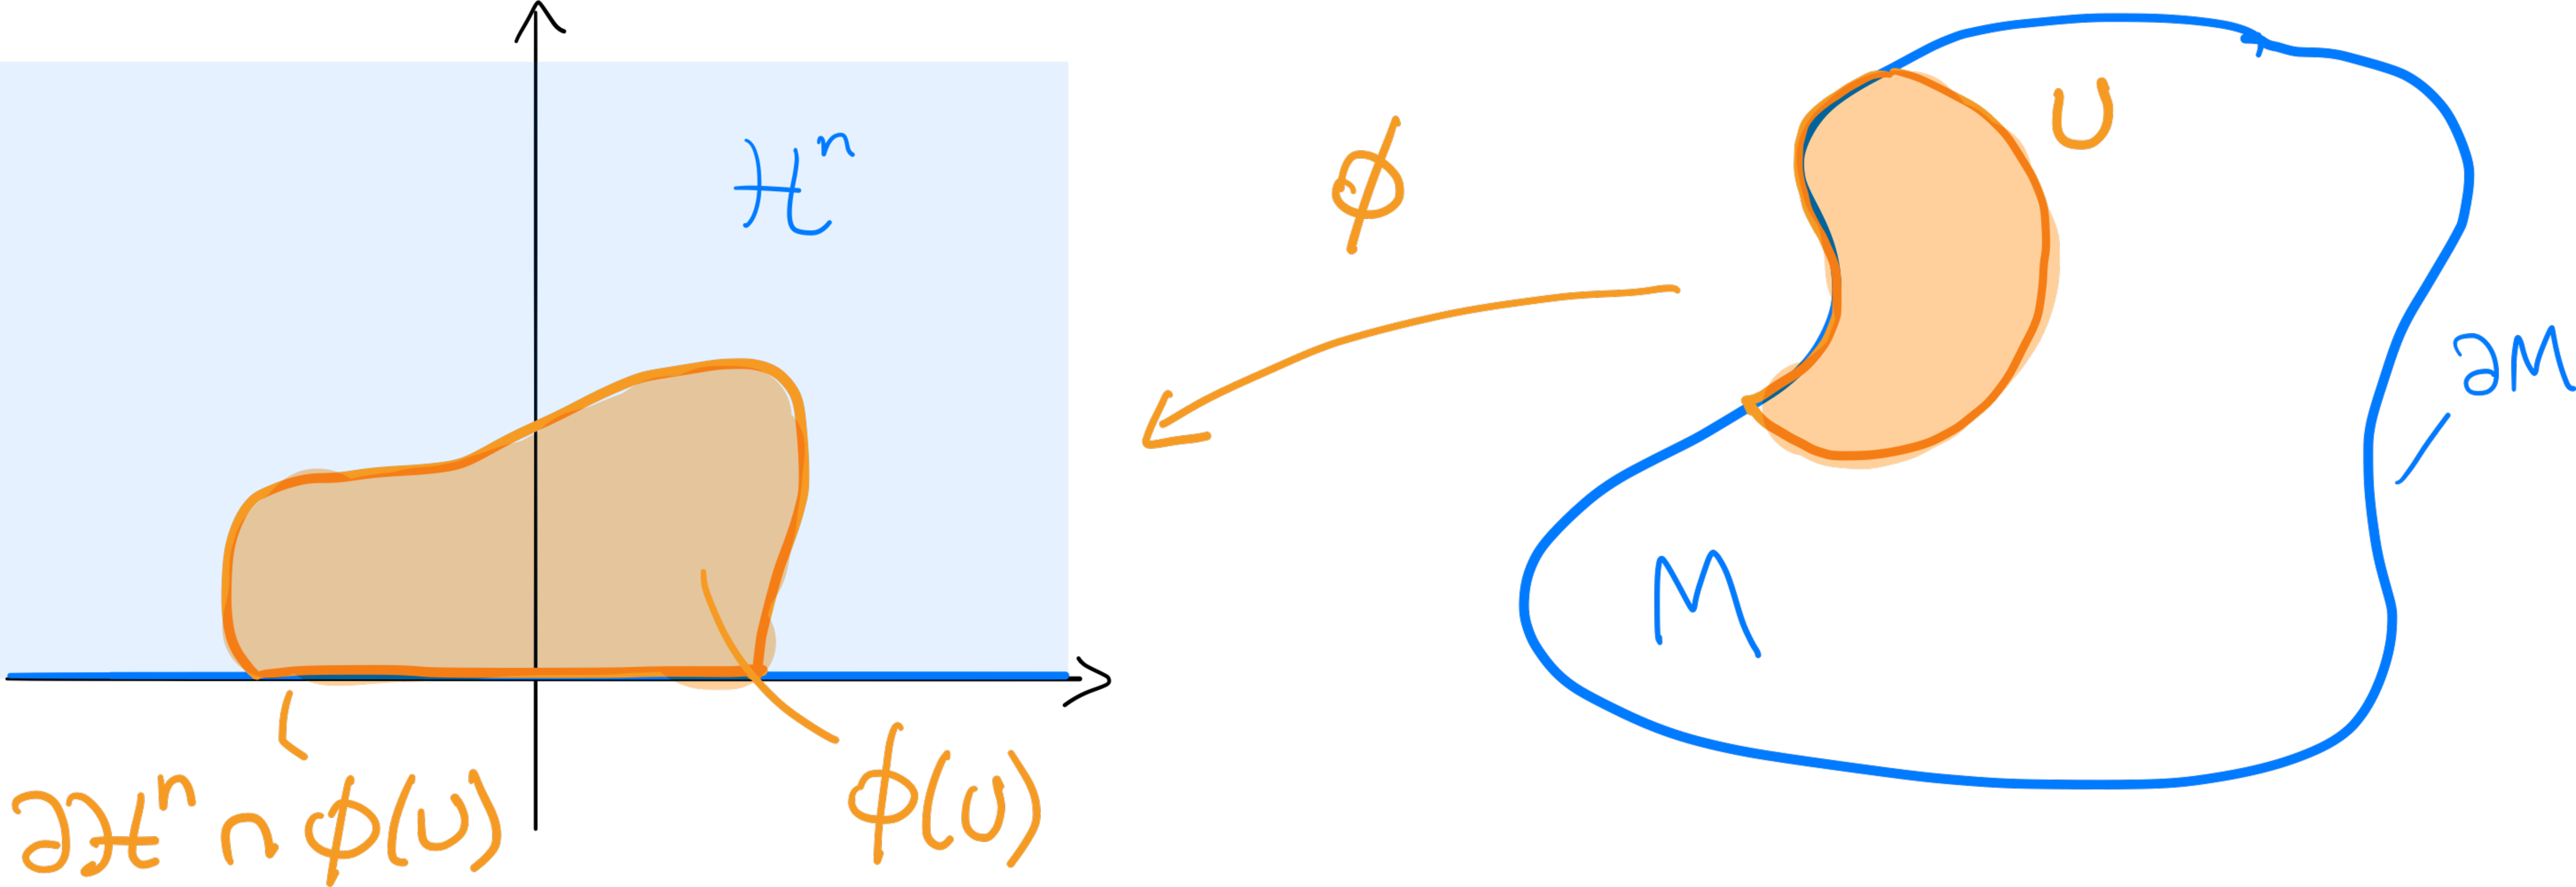
\includegraphics{1_4-mfld-w-bdry.pdf}
\end{figure}

\begin{example}\label{ex:mobius}
  A M\"obius strip $M$ is a connected $2$-manifold with boundary.
  As a topological space it is the quotient\footnote{Think of a strip of paper whose ends have been glued with a twist.} $\R\times[0,1]$ via the identification $(x,y)\sim(x+1, 1-y)$.
  The projection $\pi: [(x,y)] \mapsto (\cos(2\pi x), \sin(2\pi x))$ is a continuous surjective map to $\bS^1$.
  Given $x_0\in\R$, we can choose charts $[(x,y)]\mapsto (e^x\cos(\pi y), e^x\sin(\pi y))$ for $x\in(x_0 - \epsilon, x_0 + \epsilon)$ and any $\epsilon < 1/2$.
  \marginnote{Note that $\partial M$ is diffeomorphic to $\bS^1$. In fact, this is actually an example of a non-trivial fiber bundle, something that will make sense only a few chapters from now.
  In this case, $M$ is a bundle of intervals over a circle.}
\end{example}

We saw in Proposition~\ref{prop:uniqdiffeoinclusion} that differentiability is a local property, which means that is a property defined on open sets.
To clarify what it means to have differentiable structures on manifolds with boundary, we will thus need to clarify what it means for a function defined on $\cH^n$ to be differentiable at points on $\partial\cH^n$.
As it turns out, this is a minor modification of our previous definition that stems directly from the definition of the induced topology.

\begin{definition}
  Let $U\subset\cH^n$ be a relatively open set. A map $f: U\to\R^m$ is \emph{$r$-times continuously differentiable}, or of class $C^r$, if there exists an open set $\widetilde U\in\R^n$ and a map $\widetilde f\in C^r(\widetilde U, \R^m)$ such that $U\subset\widetilde U$ and $\widetilde f|_U = f$.
  The function $f$ is said to be \emph{smooth}, or of class $C^\infty$, if $f$ is $r$-times continuously differentiable for all $r\geq 1$.
\end{definition}

With such definition at hand, one can define compatibility, smooth atlases and differentiable structures as in Definition~\ref{def:crcomp}, Definition~\ref{def:cratlas} and Definition~\ref{def:diffstr} by considering charts taking value in $\cH^n$.

\begin{exercise}
  Explicitly state the definitions above in the case of manifolds with boundary.
\end{exercise}

\begin{definition}\label{def:diffmanifoldwb}
  \marginnote{Remember that the differentiable structure is an equivalence class of smooth atlases.}
  A \emph{smooth manifold with boundary} of dimension $n$ is a pair $(M, \cA)$ of a topological $n$-manifold with boundary $M$ and a smooth differentiable structure $\cA = \{(U_\alpha, \varphi_\alpha) \mid \alpha\in A\}$ on $M$.

  \marginnote{The boundary $\partial M$ as defined by~\eqref{def:bdry} can differ from its topological boundary as a subset of another topological space. For example the boundary $\partial\bS^1$ of the circle as a manifold is empty, but the boundary of the circle $\bS^1$ as a subset of $\R^2$ is $\bS^1$ itself.}
  The \emph{boundary} of $M$ is defined as
  \begin{equation}\label{def:bdry}
    \partial M := \bigcup_{\alpha\in A} \varphi_\alpha^{-1}\left(\varphi_\alpha(V_\alpha)\cap \partial\cH^n\right).
  \end{equation}
\end{definition}

\begin{proposition}\label{prop:bdwelldef}
  The boundary $\partial M$ is well--defined\footnote{In the sense that smooth charts send boundary pieces to boundary pieces. Note that the definition of the boundary holds for topological manifolds as well, but showing that it is well--defined is much more complicated and will be omitted.}.
\end{proposition}
\begin{proof}
  The statement follows if we show that the transition maps send boundary pieces to boundary pieces.
  It turns out that this fact is more general: for any diffeomorphism $f:U \to V$, where $U,V \subset\cH^n$ are relatively open, it holds that $x\in U\cap\partial\cH^n$ if and only if $f(x)\in V\cap\partial\cH^n$.

  Indeed, let $x\in U\cap(\cH^n\setminus\partial\cH^n)$ be a point in the interior of $U$. Expanding $f$ in Taylor series up to the first order, we have
  \begin{equation}
    f(x+h) = f(x) + Df|_x h + O(\|h\|).
  \end{equation}
  Since the total derivative $D f$ at $x$ is an isomorphism, there exist an open neighbourhood $\cO$ of $x$ such that $f(\cO)$ is open in $\R^n$ and thus $f(x)\in V\cap(\cH^n\setminus\partial\cH^n)$.
\end{proof}

\begin{remark}
  The definition of smooth maps and the propositions proven in Section~\ref{sec:smoothfn} all hold also in the case of smooth manifolds with boundary. 
\end{remark}

\begin{example}\label{ex:mfldbdryinterval}
  Let's go back to the closed interval $M=[a,b]\subset\R$. 
  With the atlas
  \begin{equation}
    \cA=\big\{
      \big([a,b), \; x\mapsto x-a\big),
      \big((a,b], \; x\mapsto b-x\big)
    \big\}
  \end{equation}
  it is a differentiable $1$-manifold with boundary $\partial M = \{a\} \cup \{b\} = \{a, b\}$.
\end{example}

Let's go back to our observation at the beginning of this section.
We started by observing that some objects seemed to be the ``sum'' of a boundary manifold and an interior manifold.
Can we make sense of such observation using our newly introduced definition?

\begin{proposition}
  Let $M$ be a differentiable $n$-manifold with boundary.
  Then $\mathring M := M\setminus\partial M$ and $\partial M$ inherit the structure of manifolds (without boundary) of dimensions $\dim(\mathring M)=n$ and $\dim(\partial M) = n-1$.
\end{proposition}
\begin{proof}
  Let $\cA = \{(U_\alpha,\varphi_\alpha) \mid \alpha\in A\}$ be an atlas for $M$. 
  Then
  \begin{equation}
    \cA_\circ := \left\{
      \left(
        U_\alpha \cap \mathring M,
        \varphi_\alpha|_{U_\alpha \cap \mathring M}
      \right) \mid \alpha\in A
    \right\}
  \end{equation}
  is an atlas for $\mathring M$ where none of the charts contain points in $\partial\cH^n$.

  In a similar vein, an atlas for $\partial M$ is given by
  \begin{equation}
    \cA_\partial := \left\{
      \left(
        U_\alpha \cap \partial M,
        \varphi_\alpha|_{U_\alpha \cap \partial M}
      \right) \mid \alpha\in A
    \right\},
  \end{equation}
  where
  \begin{equation}
    \varphi_\alpha|_{U_\alpha \cap \partial M} : (U_\alpha \cap \partial M) \to \partial\cH^n\simeq\R^{n-1}
  \end{equation}
  by the proof of Proposition~\ref{prop:bdwelldef}.
\end{proof}

\begin{example}
  Consider the cone
  \begin{equation}
    \cC = \{p=(p^1,p^2,p^3)\in\R^3 \mid (p^1)^2 + (p^2)^2 = (p^3)^2, \quad 0< p^3\leq 1\},
  \end{equation}
  with boundary $\partial\cC = \{p\in\cC \mid p^3 = 1\}$.
  \begin{marginfigure}
    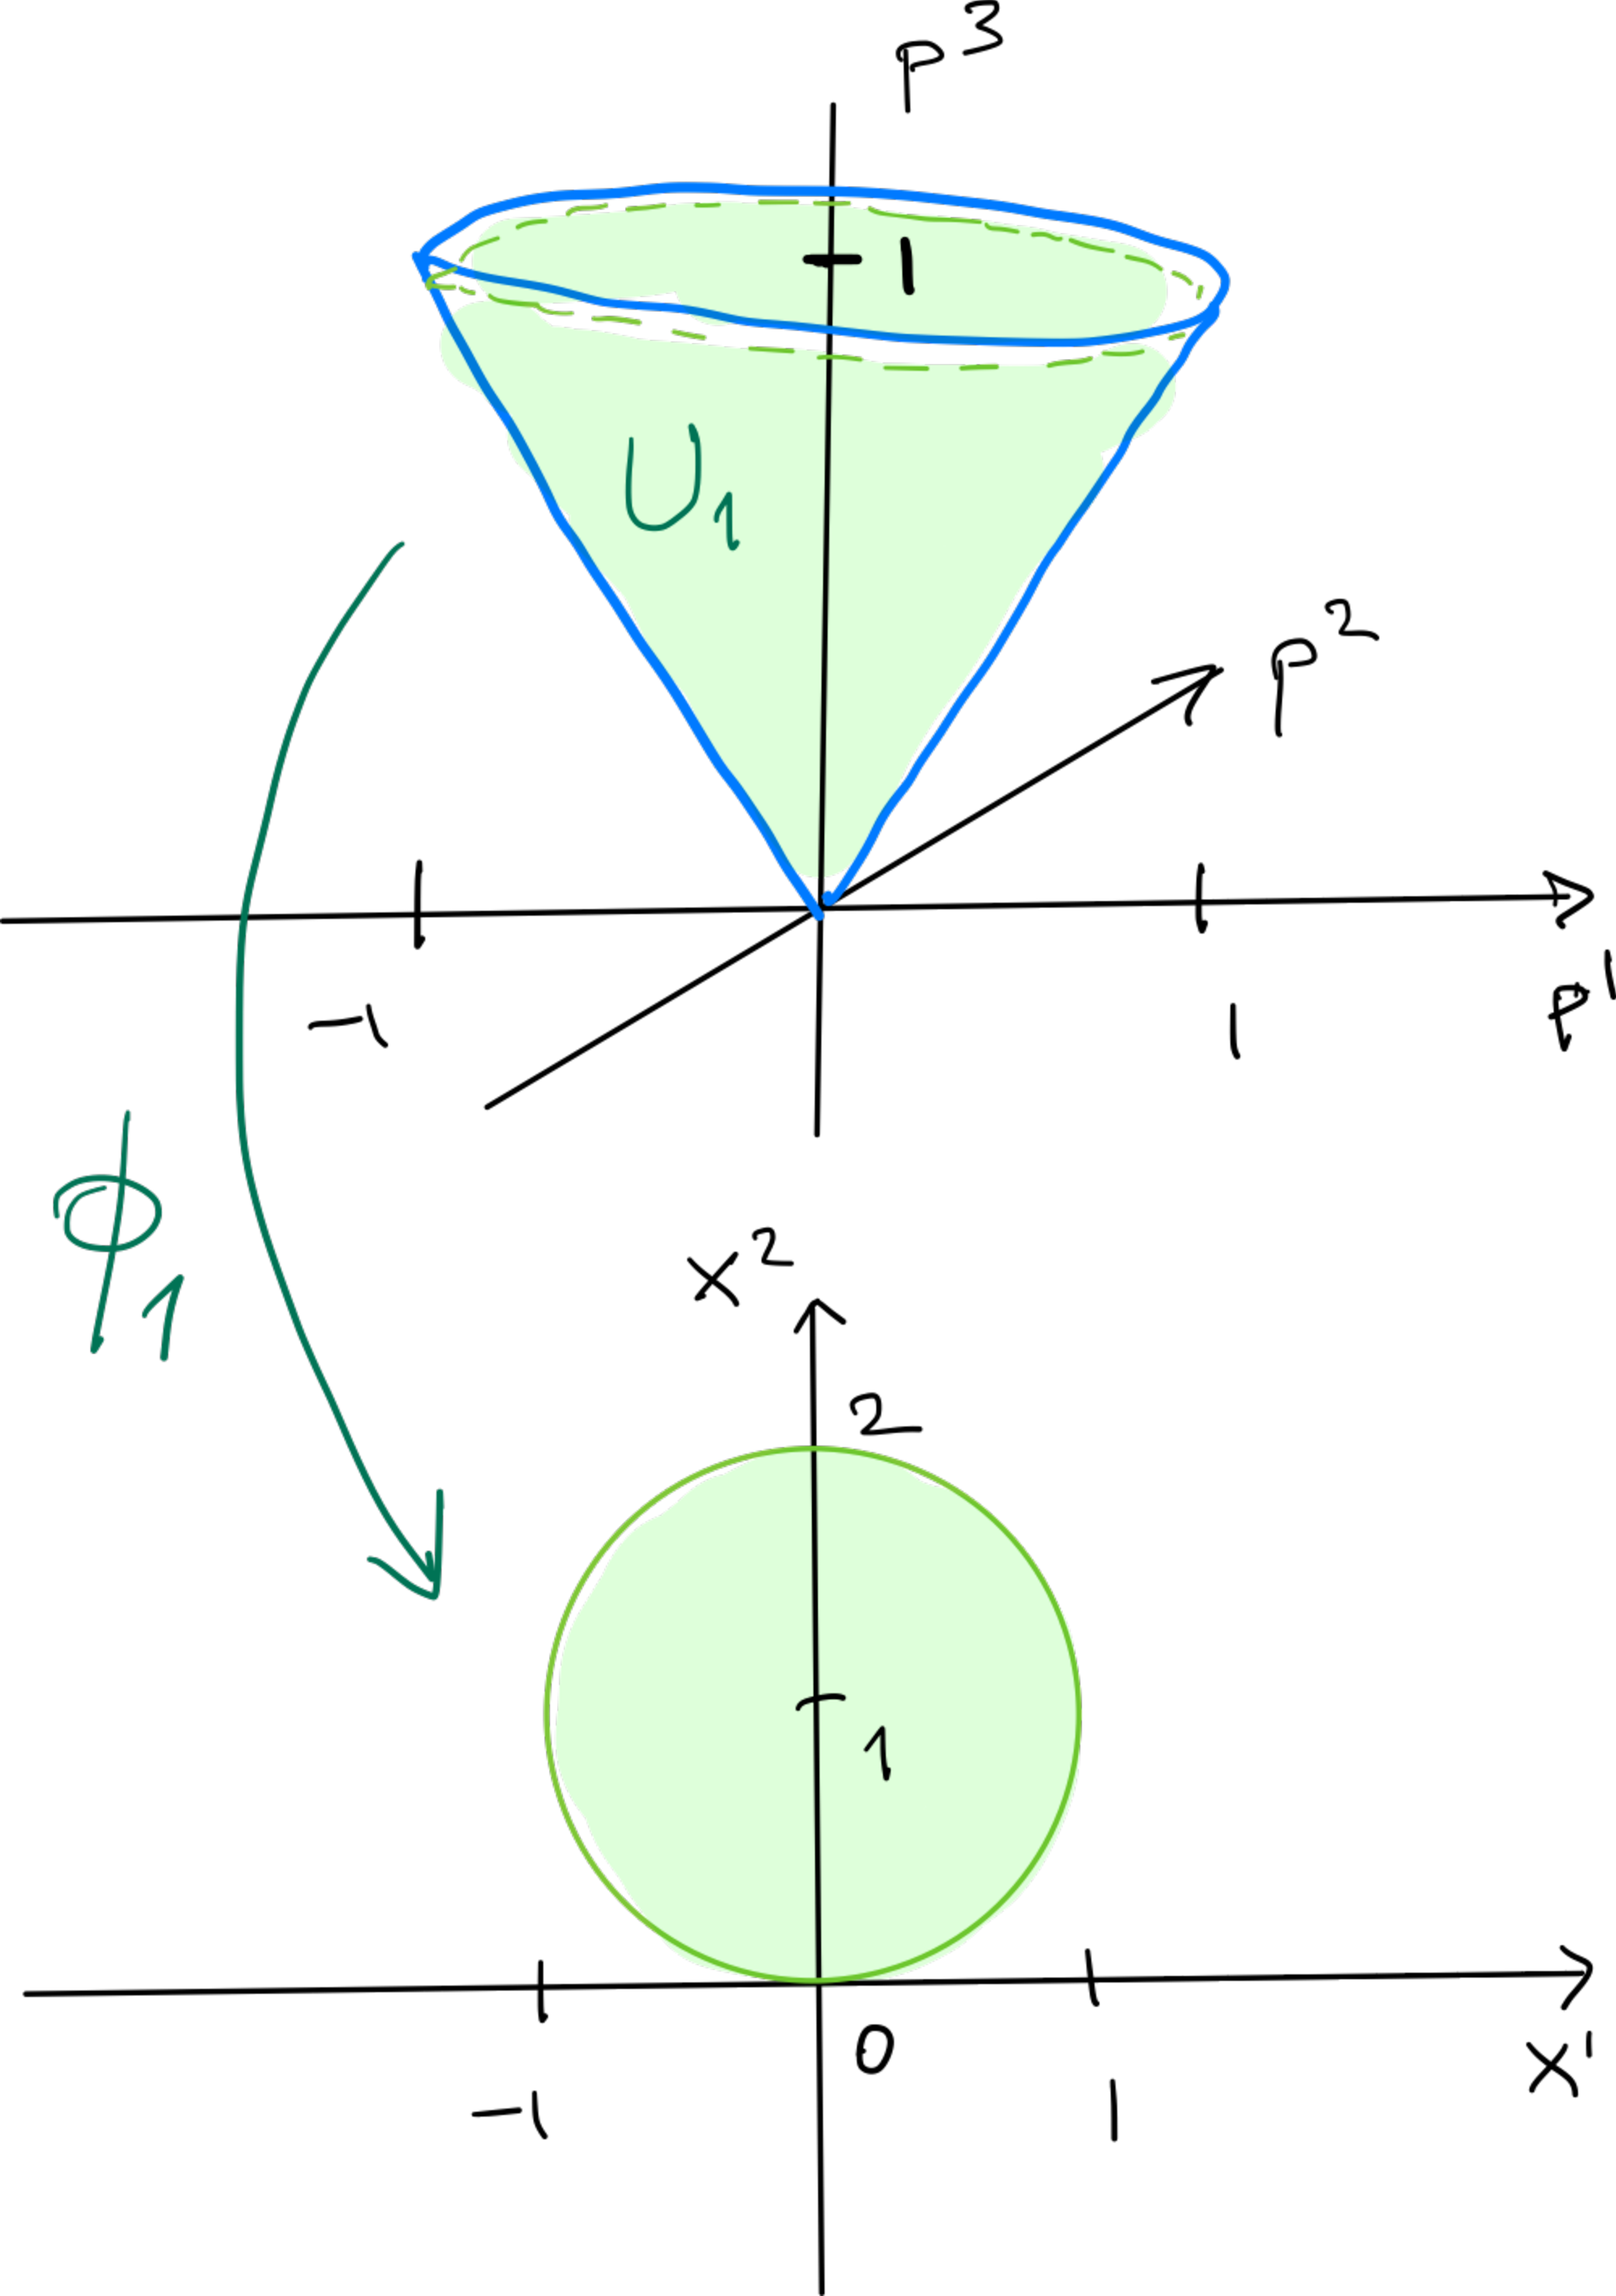
\includegraphics{1_5_9-cyl1}
  \end{marginfigure}
  We can describe the cone with the following atlas $\cA = \{(U_i,\varphi_i)\mid i=1,2,3\}$:
  \begin{itemize}
    \item $U_1 := \{p\in\cC\mid p^3 < 1\}$ with $x = (x^1, x^2) = \varphi_1(p) = (p^1,p^2+1)$, thus
      \begin{equation}
        \varphi_1^{-1}(x) = \left(x^1, x^2-1, \sqrt{(x^1)^2 + (x^2-1)^2}\right).
      \end{equation}
    \item $U_2 = \{p\in\cC\mid 1/2 < p^3 \leq 1, \; (p^1, p^2) \neq (0, p^3)\}$ with $\varphi_2$ defined as follows. Let
      \begin{equation}
        q = \psi(p) = \left(\frac{p^1}{p^3}, \frac{p^2}{p^3}, p^3\right)
        \quad\mbox{and}\quad
        \sigma(q) = \left(\frac{2q^1}{1-q^2}, 1-q^3\right),
      \end{equation}
      then $x = \varphi_2(p) = (\sigma\circ\psi)(p)$ and $\varphi_2(U_2) = \R\times[0,1/2) \subset\cH^2$.
    \item $U_3 = \{p\in\cC\mid 1/2 < p^3 \leq 1, \; (p^1, p^2) \neq (0, -p^3) \}$ and $\varphi_3$ defined similarly as in the previous point.
  \end{itemize}
  \begin{marginfigure}
    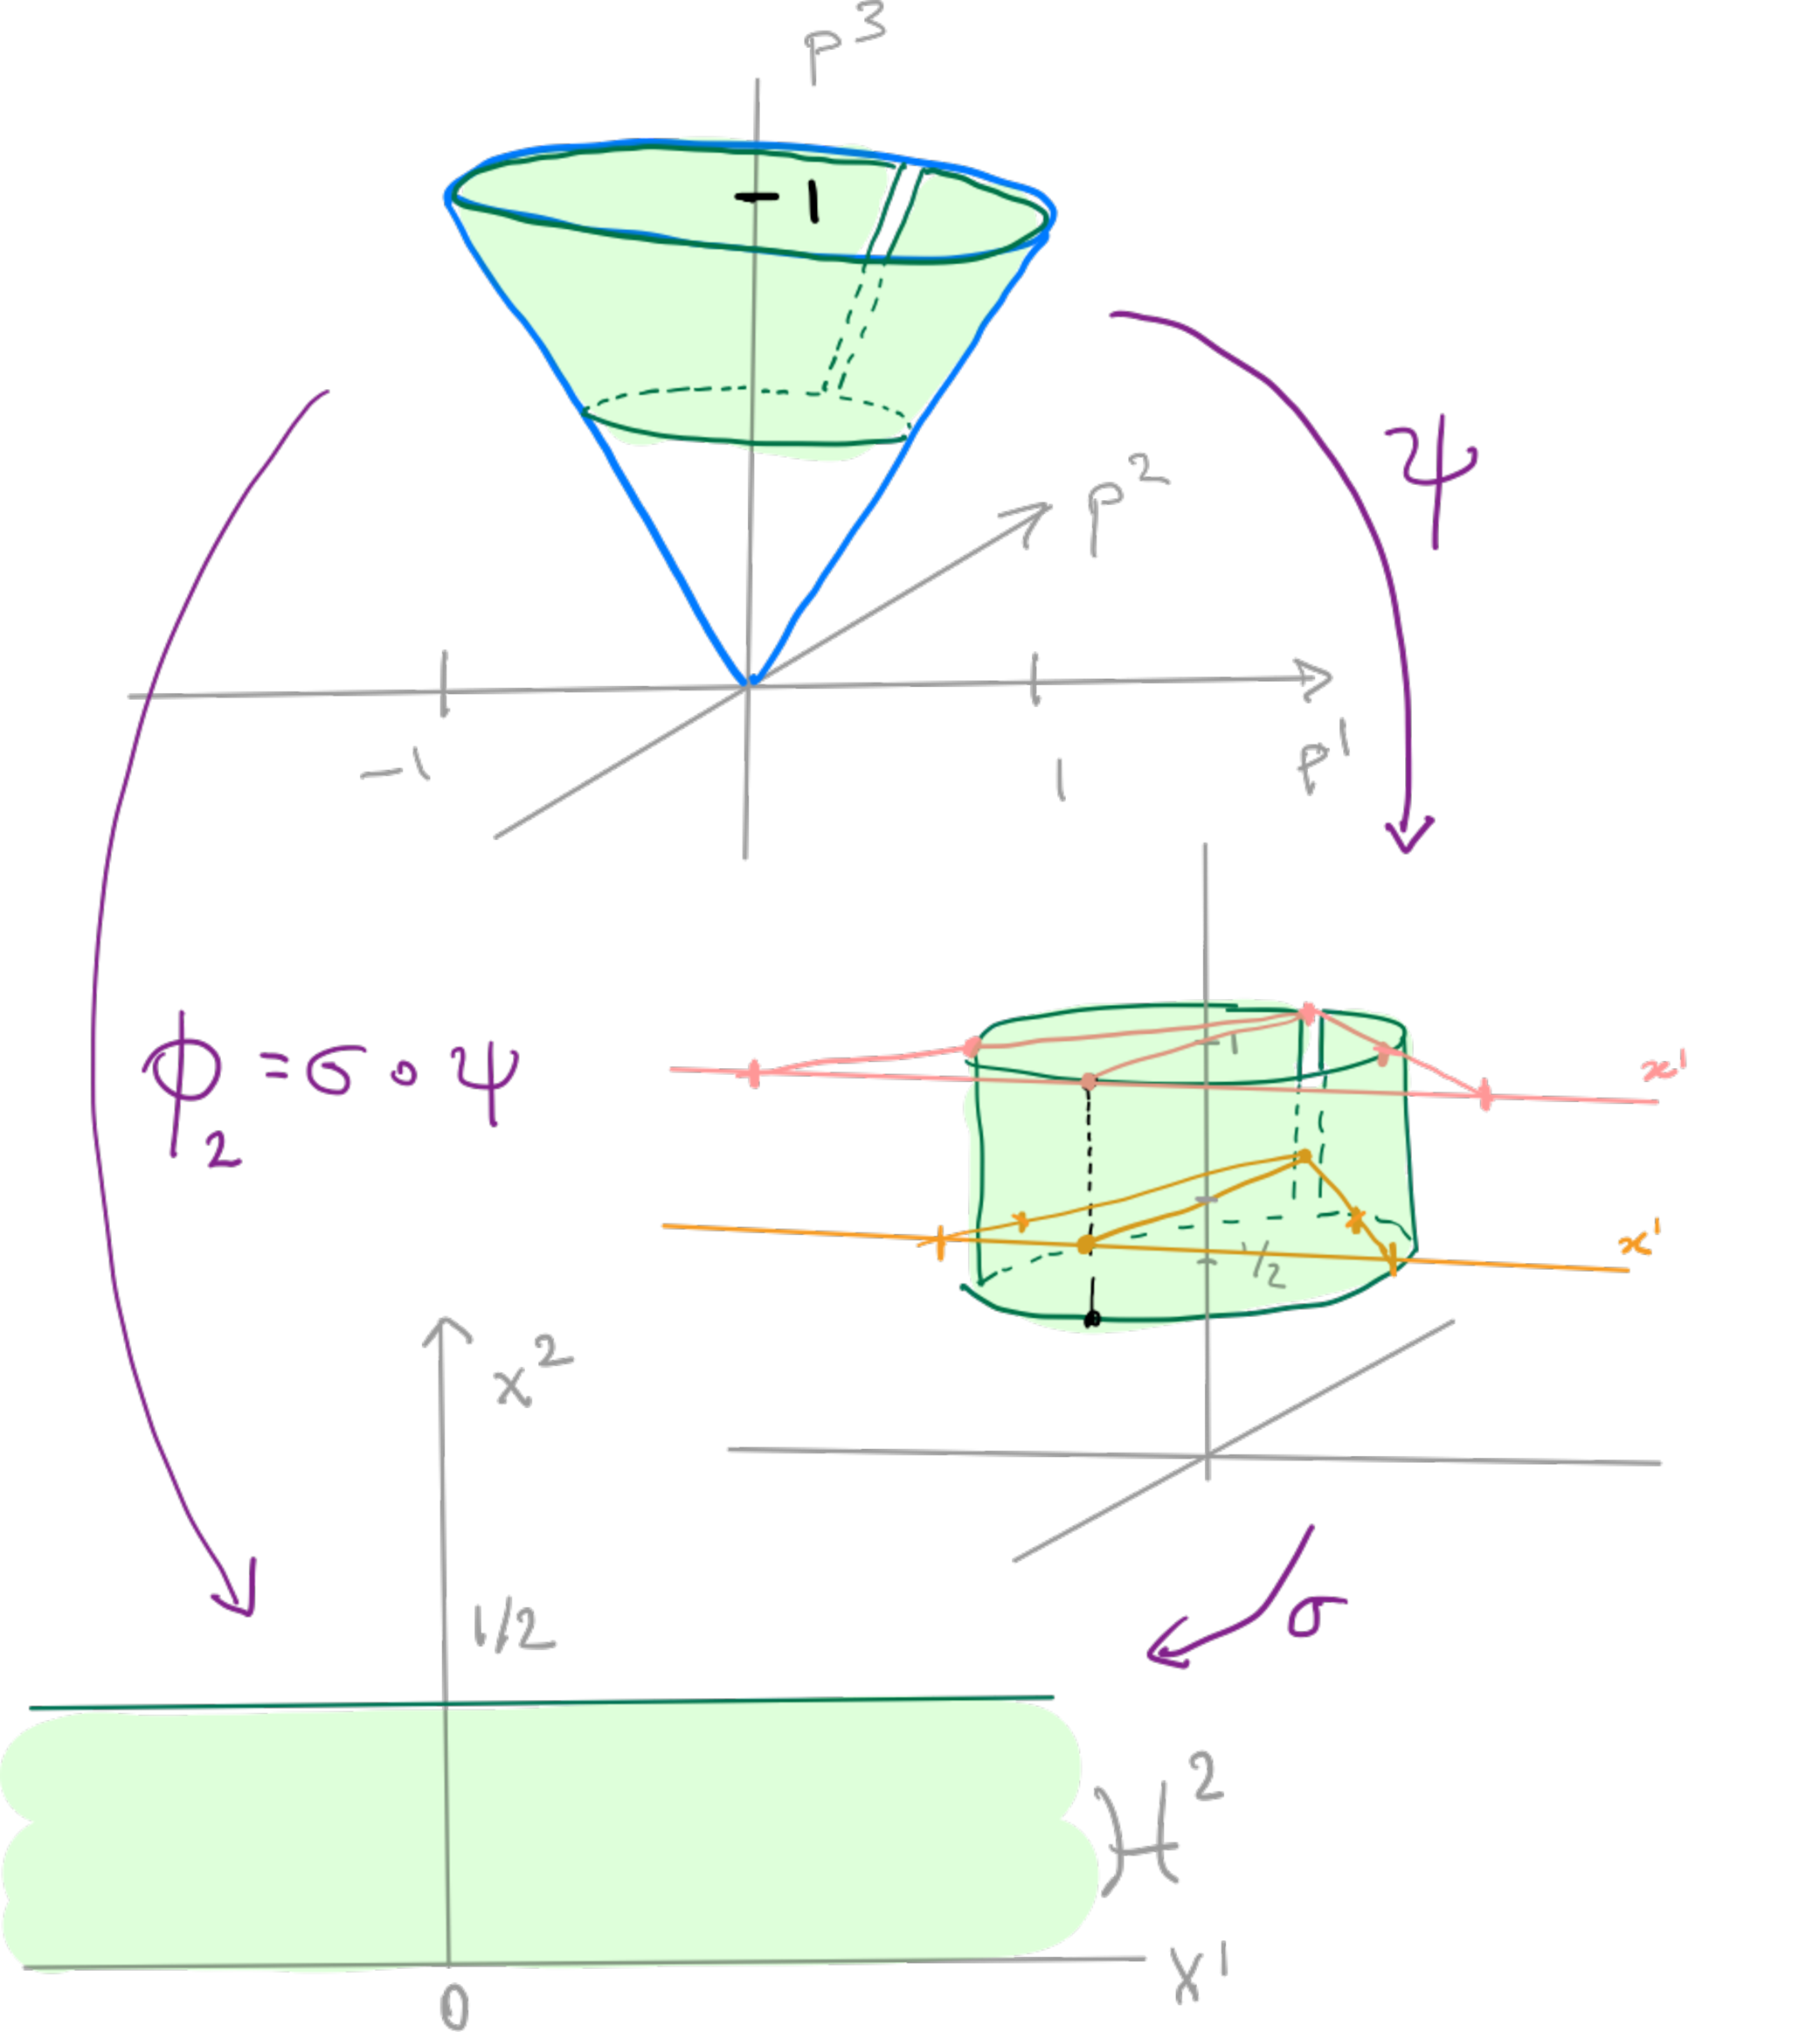
\includegraphics{1_5_9-cyl2}
    \caption{Compare $\varphi$ with the stereographic projections from Exercise~\ref{ex:stereo}. Do you notice any similarity?}
  \end{marginfigure}
  The boundary is given by $\partial\cC = \varphi_2^{-1}(\R\times\{0\}) \cup \varphi_3^{-1}(\R\times\{0\})$.
\end{example}

\begin{exercise}
  Explicitly define $\varphi_3$ from the previous example.
  Why is $\varphi_1$ not appearing in $\partial \cC$?
\end{exercise}

\begin{exercise}
  Let $M = D_1\subset \R^n$ be the $n$-dimensional closed unit ball from Example~\ref{ex:uball}.
  \begin{enumerate}
    \item Show that $M$ is a topological manifold with boundary in which each point of $\partial M = \bS^{n-1}$ is a boundary point and each point in $\mathring M = \{x\in\R^n\mid\|x\|<1\}$ is an interior point.
    \item Give a smooth structure to $M$ such that every smooth interior chart is a smooth chart for the standard smooth structure on $\mathring M$.\\
      \textit{\small Hint: consider the map $\pi\circ\sigma^{-1}:\R^n\to\R^n$ where $\sigma:\bS^n\to\R^n$ is the stereographic projection from Exercise~\ref{ex:stereo} and $\pi:\R^{n+1}\to\R^n$ is a projection that omits one of the first $n$ coordinates.}
  \end{enumerate}
\end{exercise}

\begin{tcolorbox}
  Differentiable manifolds without boundary (cf. Definition~\ref{def:diffmanifold}) can be thought as a special case of differentiable manifolds with boundary (cf. Definition~\ref{def:diffmanifoldwb}) where the boundary happens to be empty.
  Therefore, with the exception of the beginning of Chapter~\ref{ch:2}, we will no-longer distinguish the two concepts: from now on, a manifold may have or may not have a boundary.
\end{tcolorbox}


\chapter{Tangent bundle}\label{ch:2}
\section{Let the fun begin!}
\newthought{We are left to define derivatives} of functions between manifolds.
And, since we saw that euclidean spaces are manifolds, we better find a definition that coincides with the one you saw in your analysis courses.

\begin{marginfigure}[7em]
  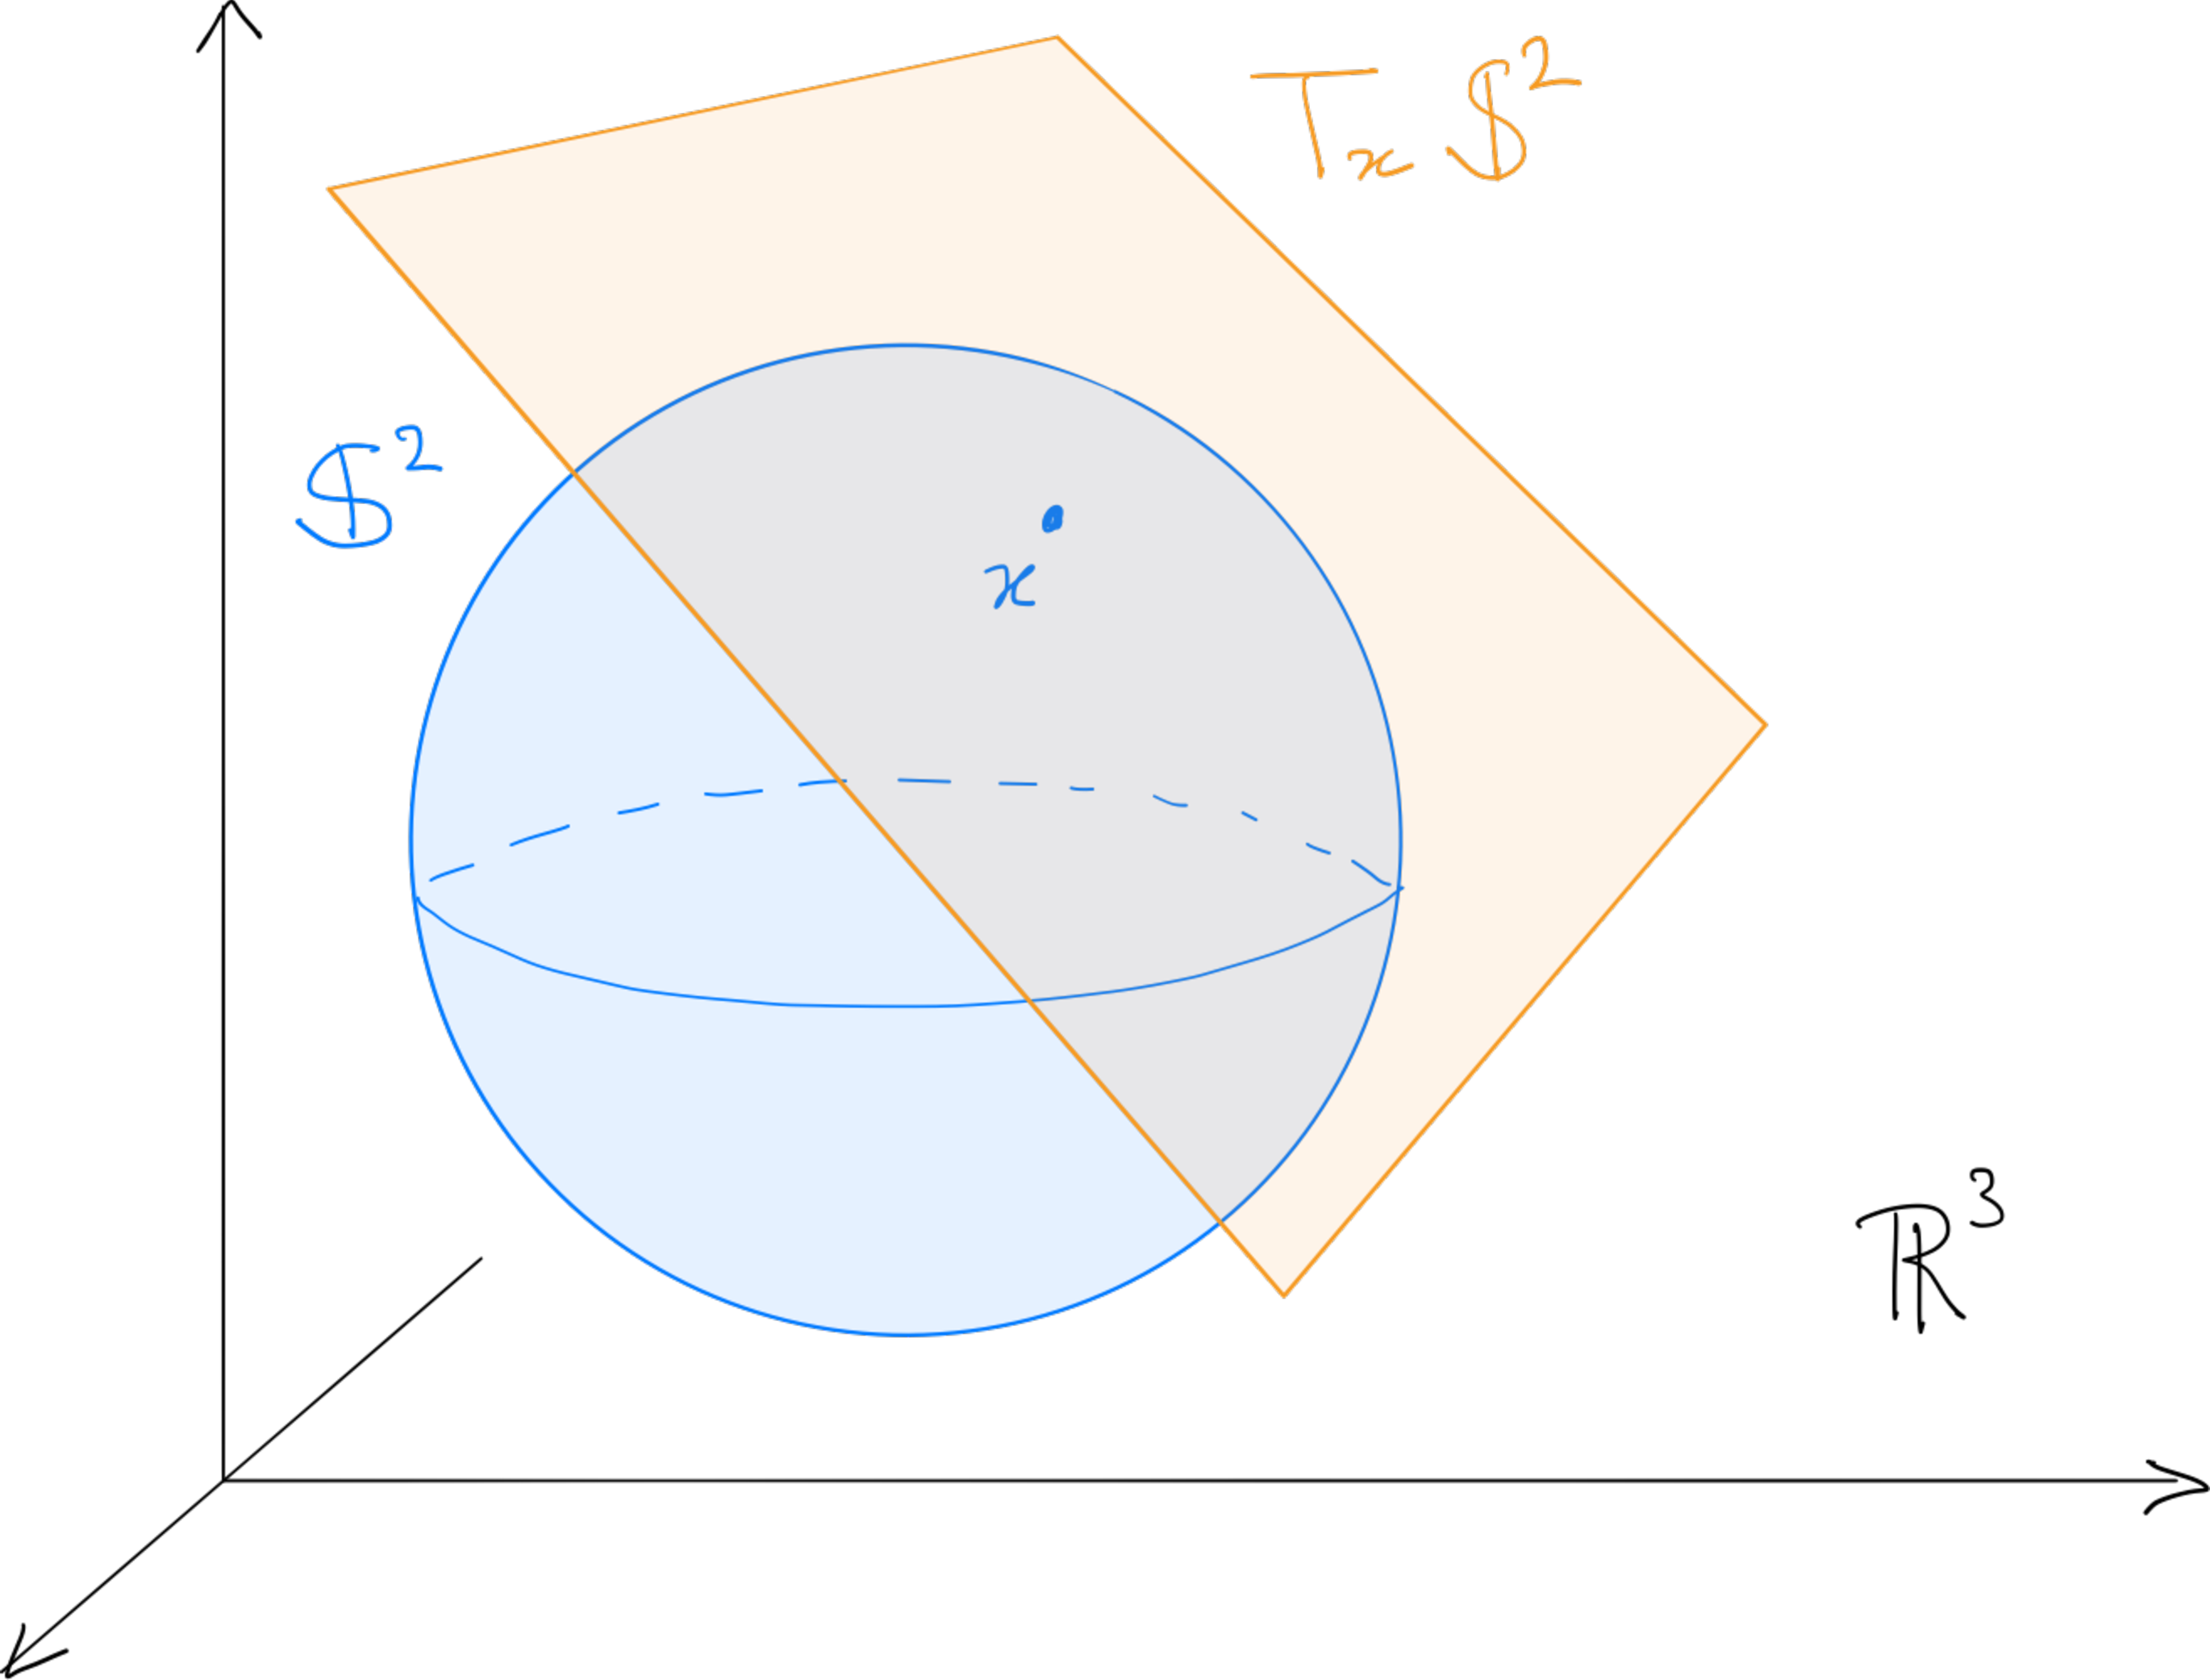
\includegraphics{2_1-embedded-sphere-tangent.pdf}
  \label{fig:tan-embedded-sphere}
  \caption{Tangent space to a point of a sphere $\bS^2$ embedded into the ambient space $\R^3$.}
\end{marginfigure}
In this chapter we will see how to associate to an $n$-dimensional smooth manifold $M$ an $n$-dimensional vector space, denoted by $T_x M$, to each point $x\in M$.
Such vector space is called \emph{tangent space to $M$ at $x$} and, for a manifold embedded into a euclidean ambient space, it will coincide with the intuitive understanding of a tangent hyperplane to the point on the manifold, see also Figure~\ref{fig:tan-embedded-sphere}.
As we will see, there are various different definition of tangent space but, in the end, they all turn out to be equivalent.

Due to a certain amount of freedom in terms of different ``perspectives'' leading to different but equivalent definitions, there is no unique way of introducing tangent spaces.
Just to give you an idea, all the following approaches lead to equivalent definitions (see also~\cite{book:lee}):
\begin{itemize}
  \item equivalence classes of curves through a point;
  \item transformation laws of the components of vectors with respect to different charts;
  \item generalization of linear approximation into the idea of an abstract derivation;
  \item derivations in the category of germs of functions;
\end{itemize}

It is also possible to ``flip'' the whole construction around, constructing differentials and cotangent spaces and using them to introduce the tangent spaces.
This is the approach taken by~\cite{lectures:hitchin} and it is at least worth of a look if you want to see a different perspective.

To avoid diverging from~\cite{book:tu} too much\footnote{Since it used to be the compulsory reading material in the previous years.}, we will stick to derivations on the space of germs, which emphasizes the locality of derivations to an extreme.
The equivalence between our approach and the one based on charts will be left as homework, while we will look into the equivalence with the speed of curves and with derivations together.

\section{Directional derivatives in euclidean spaces}\label{sec:dd}

Suppose that $f: U\subset\R^n\to\R^k$ is a smooth map defined on an open subset $U\subset \R^n$.
In multivariable calculus you have seen that if $x\in U$ and $v\in\R^n$, then the vector $Df(x) v$ can be interpreted as the directional derivative\footnote{Sometimes this is denoted $D_v f(x)$ instead.} of $f$:
\begin{equation}
  Df(x) v = \lim_{t\to0}\frac{f(x+tv) - f(x)}{t}.
\end{equation}
Then, the partial derivative is obtained as the particular case
\begin{equation}
  D_jf(x) := Df(x) e_j = \lim_{t\to0} \frac{f(x+te_j) - f(x)}{t}.
\end{equation}
Of course, we can also look at the derivative by using the standard euclidean coordinates $r^1, \ldots, r^n$, in that case we would be deriving $r^i \circ f : \R^n \to \R$.

\newthought{Let's take it slow}, and compare all these various derivatives next to each other.
For $f:U\subset\R^n\to\R^k$ and $x\in U$, we have
\begin{marginfigure}[3.5cm]
  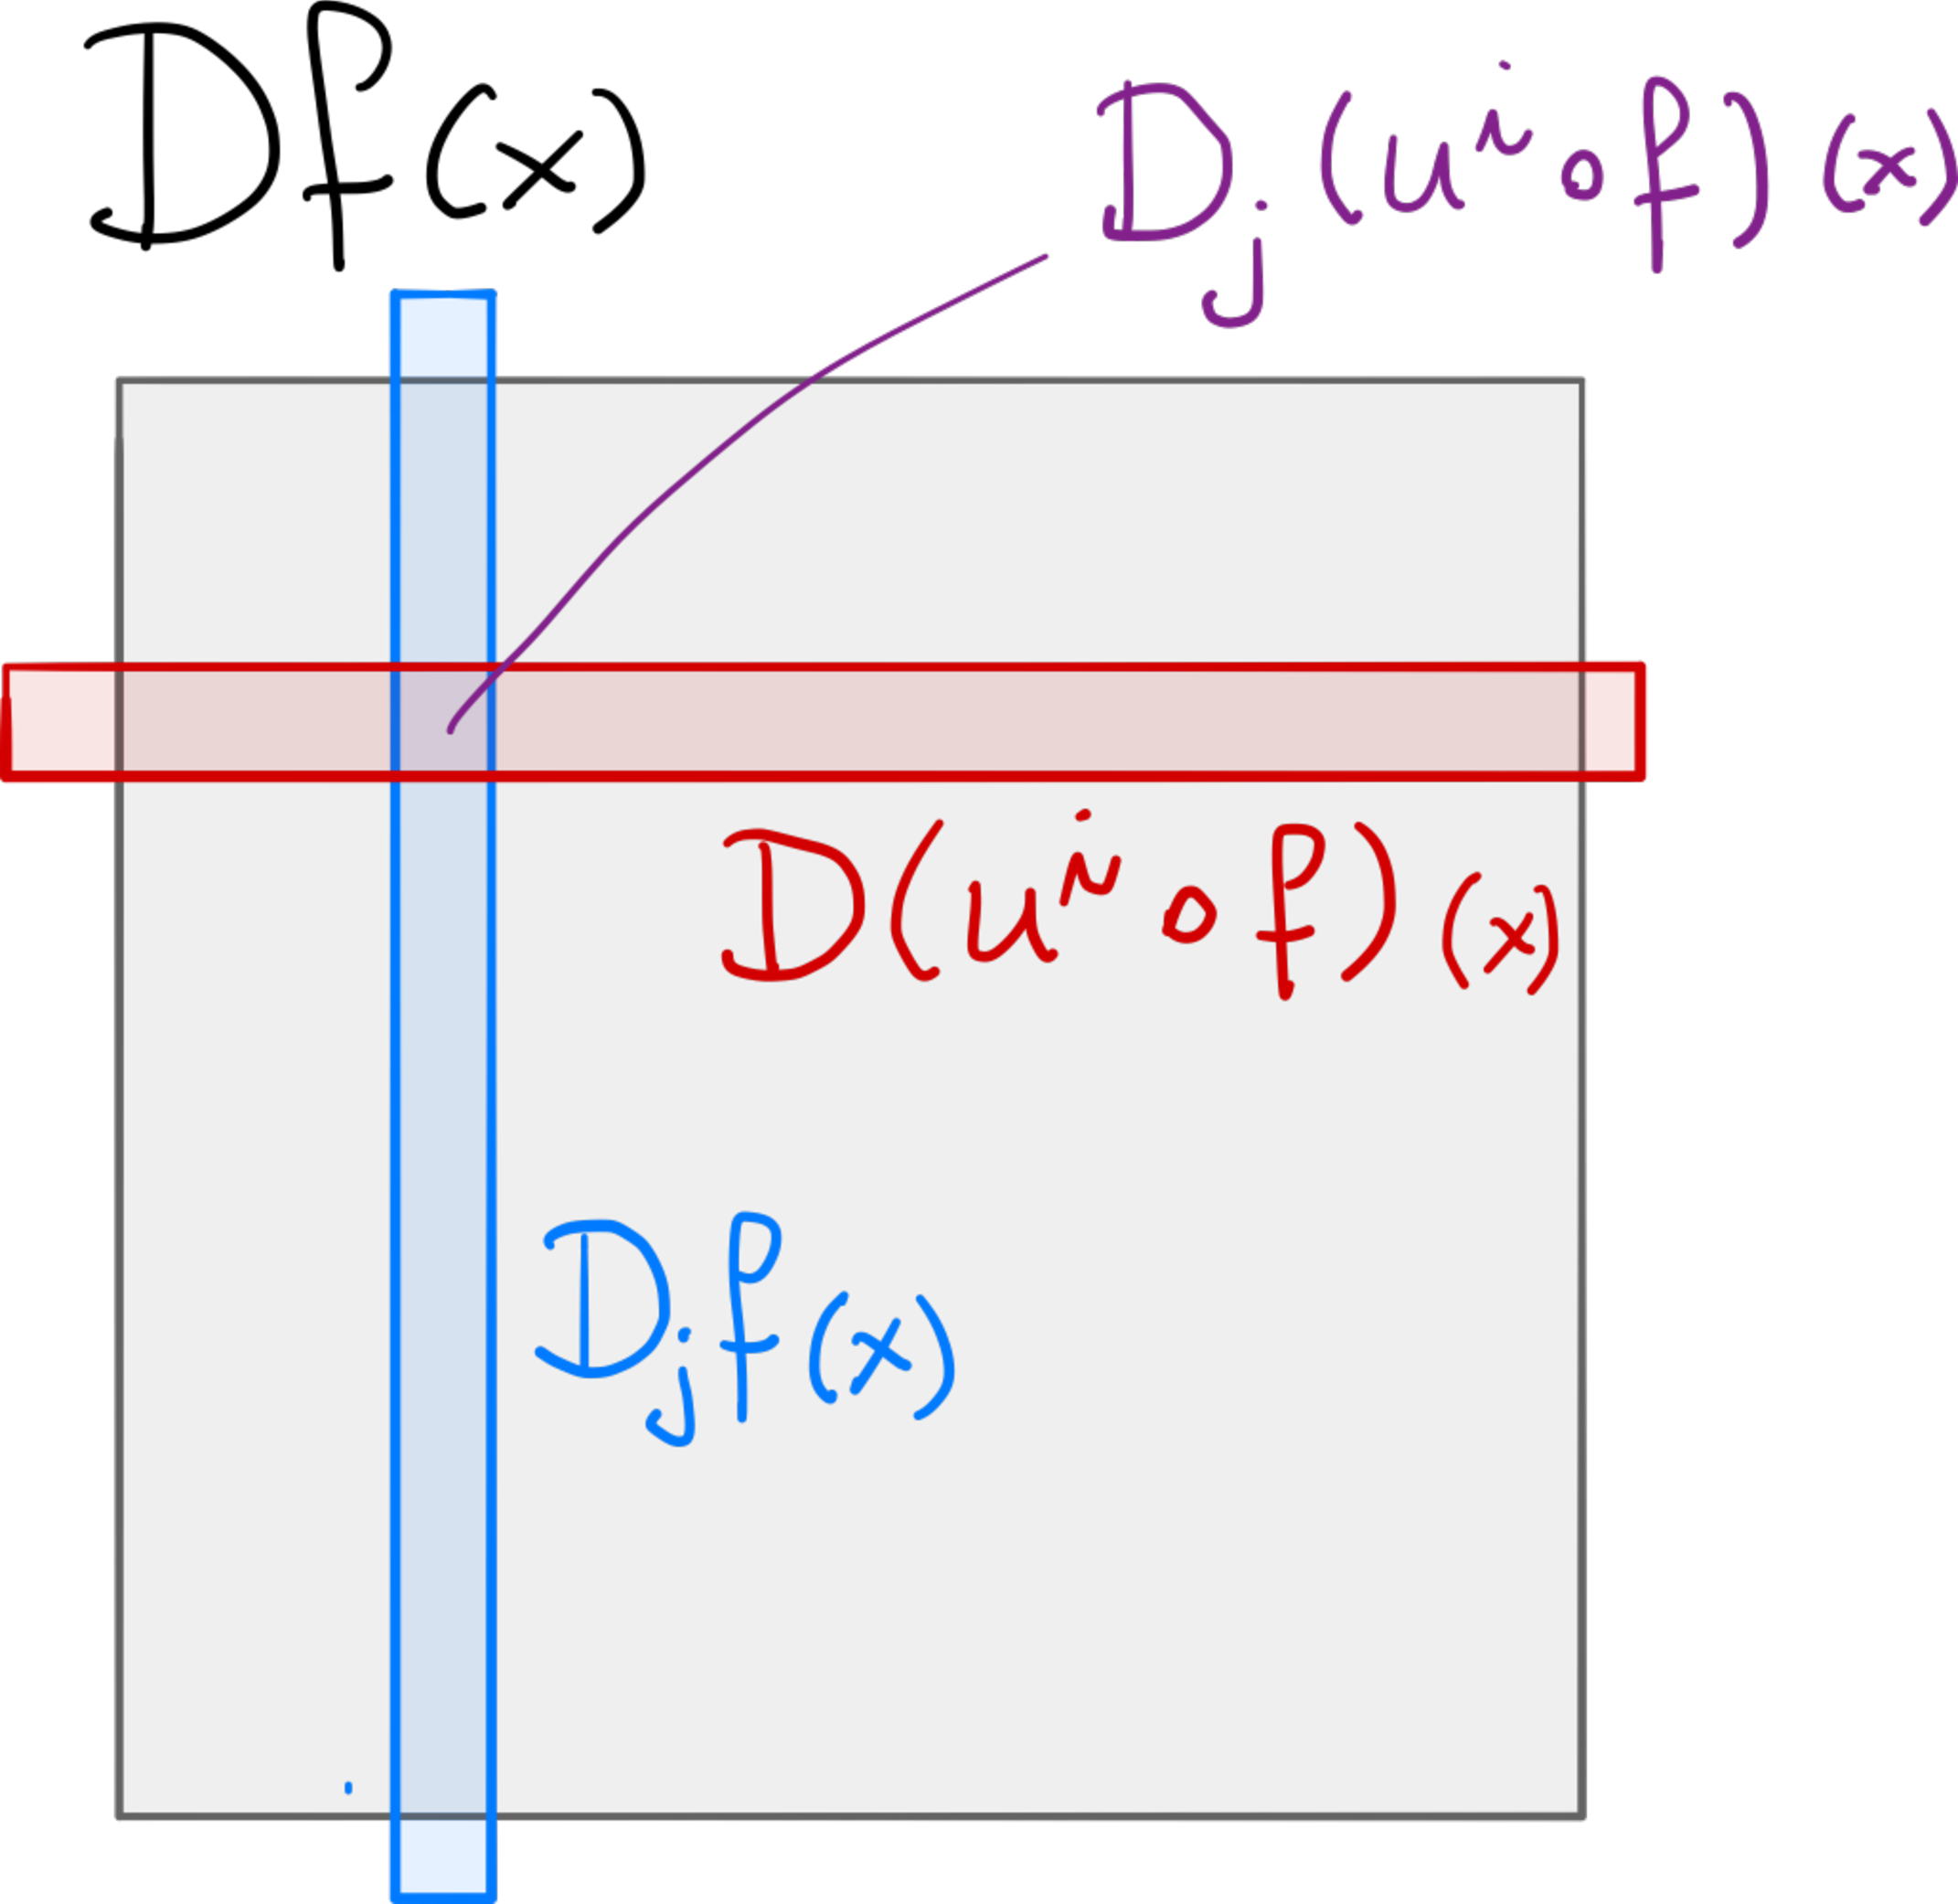
\includegraphics{2_3-ederivs.pdf}
\end{marginfigure}
\begin{itemize}
  \item $Df(x)$, the Jacobian matrix, which is a $k\times n$ matrix;
  \item $D_j f(x)$, the $j$th column of the matrix $Df(x)$, which is an element of $\R^k$;
  \item $D(r^i\circ f)(x)$, a linear function from $\R^n \to \R$, which one can think as the $i$th row of the matrix $Df(x)$;
  \item $D_j(r^i\circ f)(x) = \frac{\partial f^i}{\partial x^j}(x)$, a number in $\R$, which corresponds to the $(i,j)$th element $(Df(x))_j^i$ of the matrix $Df(x)$.
\end{itemize}

This notation using $D$ instead of spelling out the partial derivatives, comes with an important advantage.
Let's use it to rewrite the chain rule form Proposition~\ref{thm:chainrule}(\ref{thm:chainrule2}):
\begin{equation}
  D_j(r^i\circ g \circ f) (x) = \sum_{l=1}^k D_l(r^i\circ g)(f(x))\; D_j(r^l \circ f)(x),
\end{equation}
\marginnote[-4em]{Using Einstein notation, since $l$ is the only index that appears both in lower and upper position, $D_j(r^i\circ g \circ f) (x) = D_l(r^i\circ g)(f(x))\; D_j(r^l \circ f)(x)$.}
where $1\leq i\leq m, 1\leq j \leq n$.
As you can see, we do not need to explicitly spell out the derivatives in local coordinates on $\R^n$ or $\R^k$ in this new formula.
This will prove extremely convenient for the development of the theory.

\section{Germs and derivations}

\newthought{To reach our goal of defining derivations on manifolds}, a direct extension of partial derivatives is not enough: we will need to introduce some more levels of abstraction.

\begin{definition}
  Let $M$ be a smooth manifold.
  For some point $p\in M$, let $U,V\subset M$ be two neighbourhoods of $p$.
  We say that two functions $f\in C^\infty(U)$ and $g\in C^\infty(V)$ have the same \emph{germ} at $p$ if there exists a neighbourhood $W\subset U\cap V$ of $p$ such that $f|_W \equiv g|_W$.
\end{definition}

Germs define an equivalence relation on the set of smooth functions defined on a neighbourhood of a point $p$: $(U, f) \sim_p (V, g)$ if they have the same germ at $p$. Then, a germ $[f]_p$, where $(U, f)$ is one representative for $[f]_p$, is an equivalence class in the quotient space 
\begin{equation}
  C_p^\infty(M) := C^\infty(M)/\!\sim_p.
\end{equation} 

\begin{exercise}
  Show that $\sim_p$ defined above is an equivalence relation in $C^\infty(M)$.
\end{exercise}

For $c\in\R$ and $[f]_p, [g]_p$ germs with representatives $(U, f), (V, g)$, we have
\begin{itemize}
  \item $[f]_p + [g]_p$ is the germ with representative $(U\cap V, f+g)$;
  \item $[f]_p [g]_p$ is the germ with representative $(U\cap V, f g)$;
  \item $c[f]_p$ is the germ with representative $(U, cf)$.
\end{itemize}
Therefore, $C_p^\infty(M)$ is also an algebra over $\R$.

\begin{exercise}
  Check that the operations above are well--defined.
\end{exercise}

Germs are the apotheosis of locality: a germ at $p$ has a well--defined value at $p$ and nowhere else.
This results in a map,
\begin{equation}
  \eval_p: C_p^\infty(M) \to \R, \quad
  \eval_p([f]_p) := f(p),
\end{equation}
where $(V,f)$ is any representative of $[f]_p$.
\begin{exercise}
  Check that the $\eval_p$ map is well--defined.
\end{exercise}

We can now go back to our discussion of euclidean derivations to motivate our definition of tangent vectors.

\begin{example}\label{ex:euclideanD}
  Let $U\subset\R^n$ open\footnote{In what follows, we will think at $U$ both as an open subset of $\R^n$ and a smooth manifold depending on what is most convenient for us.} and $f\in C^\infty(U)$.
  For $x\in U$ and $v\in\R^n$ we have seen that $Df(x)$ can be interpreted as a matrix that consumes the vector $v$ to produce a number $D(f)v$.
  In such interpretation $f$ is fixed and only $x$ and $v$ vary, however there is no reason for this restriction.

  Indeed, an alternative interpretation lets also $f$ vary and consider the action of differentiation as a map
  \begin{equation}
    U \times \R^n \times C^\infty(U) \to \R,\quad
    (x,v,f) \mapsto Df(x) v.
  \end{equation}
  And since we are flipping around all the ideas, let us consider $x$ and $v$ fixed and instead only let $f$ vary:
  \begin{equation}\label{eq:mapxvtoD}
    (x,v):C^\infty(U) \to\R, \quad (x,v)(f) := Df(x)v.
  \end{equation}
  By the definition~\eqref{eq:diff} of the euclidean differential, we know that it is a local property: the value $Df(x)$ only depends on the germ of $f$ at $x$.
  Thus we can rephrase~\eqref{eq:mapxvtoD} by saying that $v$ defines a \emph{linear} map
  \begin{equation}
    v : C_x^\infty(U) \to \R, \quad
    v([f]_x) := Df(x) v.
  \end{equation}
  In fact, this is not just a linear map, it also satisfies a \emph{derivation} property, in the sense that
  \begin{equation}
    v([f]_x [g]_x) =
      \eval_x([f]_x)v([g]_x)
      + \eval_x([g]_x)v([f]_x).
  \end{equation}
  Which, rewritten in a more familiar form, is just a way to rewrite the \emph{Leibniz rule}:
  \begin{equation}
    D(fg)(x) v = f(x)Dg(x)v + g(x) Df(x)v.
  \end{equation}

  Note that we have now two different interpretations for $v$: it is both a vector in $\R^n$ and a linear map $C_x^\infty(U) \to \R$ satisfying the derivation property.
\end{example}

Motivated by Example~\ref{ex:euclideanD}, we will define a tangent vector as a derivation on the space of germs.

\begin{definition}
  Let $M$ a smooth manifold of dimension $n$ and let $p\in M$.
  A \emph{tangent vector at $p$} is a linear map
  \marginnote{Keep always in mind that the value $v([f]_p)$ only depends on the value of $f$ around the point $p$.}
  \begin{equation}\label{def:tangentvector}
    v: C_p^\infty(M)\to\R
  \end{equation}
  which is also a derivation, i.e.
  \begin{equation}
    v([f]_p [g]_p) =
      \eval_p([f]_p)v([g]_p)
      + \eval_p([g]_p)v([f]_p).
  \end{equation}

  Since a tangent vector is a linear map from the vector space $C_p^\infty(M)$ to $\R$, the set of all tangent vectors at a point $p$ is itself a vector space\footnote{Exercise: why is this true?} which we denote by $T_p M$.
\end{definition}

Let's check that these vectors, at least satisfy the most elementary properties of derivations: one would expect the derivative of constant functions to be zero, is that the case?

\begin{lemma}\label{lem:f'0is0forconst}
  Let $M$ be a smooth manifold, let $U\subset M$ be an open set containing $p$ and let $v\in T_p M$.
  Denote by $[c]_p$ the germ of a constant function $(U, p \mapsto c)$.
  Then $v([c]_p) = 0$.
\end{lemma}
\begin{proof}
  Since $[c]_p = c [1]_p$, by linearity we have $v([c]_p) = c v([1]_p)$.
  Thus, it will be enough to show that $v([1]_p) = 0$.
  Since $v$ is a derivation, using the algebra properties of the space of germs we get
  \marginnote{Keep this simple trick in mind, it will be useful in the future.}
  \begin{equation}
    v([1]_p) = v([1]_p [1]_p) = 2 \eval_p([1]_p)v([1]_p) = 2 v([1]_p).
  \end{equation}
  Thus, $v([1]_p) = 0$, concluding the proof.
\end{proof}

As you can see, working with equivalence classes is doable but unnecessarily cumbersome.
As we did with atlases, we would like to get it over with.

\begin{definition}
  Let $M$ be a smooth manifold and $p\in M$.
  Let $W\subseteq M$ be any neighbourhoods of $p$.
  \marginnote{We are still talking about derivations of functsion at specific points, not to be confused with the derivations of the algebra $C^\infty(W)$ which we will introdce later and will be maps of the kind $C^\infty(W)\to C^\infty(W)$.}
  A map $w:C^\infty(W)\to\R$ is called a \emph{derivation of $C^\infty(W)$ at $p$} if it is linear over $\R$ and satisfies Leibniz rule
  \begin{equation}
    w(fg) = f(p)w(g) + g(p)w(f).
  \end{equation}
\end{definition}

If $v\in T_p M$, then we already saw that $v$ naturally defines a derivation $w$ of $C^\infty(W)$ for any open neighbourhood $W$ of $p$.
In this case
\begin{equation}\label{eq:derivfromtg}
  w(f) := v([f]_p).
\end{equation}
Showing that the opposite is also true will require a bit of work.

\begin{proposition}
  Let $M$ be a smooth manifold, $p\in M$ and $W$ any neighbourhood of $p$.
  Then there is a linear isomorphism between $T_p M$ and the space of derivations of $C^\infty(W)$ at $p$.
\end{proposition}
\begin{proof}
  To prove the theorem we need to invert~\eqref{eq:derivfromtg} and define a tangent vector in terms of of a derivation of $C^\infty(W)$ at $p$.
  We will proceed in three steps

  \newthought{Step I}. Let $w:C^\infty(W) \to\R$ be a derivation at $p$ and suppose that $f\in C^\infty(W)$ is identically zero on a neighbourhood $W_0\subset W$ of $p$. We are going to show that $w(f)=0$.

  By Proposition~\ref{prop:cutoff}, we can find a cutoff function $\rho:M\to\R$ such that $\rho(p)=1$ inside $W_0$ and $\supp(\rho) \subset W_0$. Consider now $g = \rho f : W \to \R$. Then $g$ is identically zero in the whole $W$, and thus\footnote{Follows by linearity, exactly as in Lemma~\ref{lem:f'0is0forconst}} $w(g) = 0$. Using Leibniz rule, the fact that $\rho(p)=1$ and $f(p) = 0$, we get
  \begin{equation}
    0 = w(g) = w(\rho f) = \rho(p) w(f) + f(p)w(\rho) = w(f).
  \end{equation}

  \newthought{Step II}.
  Let $[f]_p\in C_p^\infty(M)$.
  We want to show that it is always possible to find a representative for $[f]_p$ with domain $W$, that is, there exists $g\in C^\infty(W)\to\R$ such that $[g]_p = [f]_p$.
  Let $(V, f)$ be any representative of $[f]_p$.
  Since germs are local, if necessary, we can shrink $V$ so that $V\subset W$.
  Here comes the tricky bit: we need to extend $f$ to a function $g$ defined on $W$ which coincides with $f$ in some neighbourhood of $p$!
  To this end, choose\footnote{We can do this because topological manifolds are locally compact Hausdorff spaces, which implies that every point has a neighbourhood with compact closure. You can take it for granted or have a look at e.g.~\cite[Lemma 4.65]{book:lee:topology} or~\cite{book:munkres:topology}.} a smaller neighbourhood $U$ of $p$ such that $\overline{U}\subset V\subset W$.
  Again, Proposition~\ref{prop:cutoff} comes to the rescue. Apply it with $K=\overline{U}$ and ``$U$'' equal to $V$, and consider
  \begin{equation}
    g:W\to\R, \quad
    g(q) := \begin{cases}
      \rho(q)f(q), & q\in V,\\
      0, & q \in W\setminus V.
    \end{cases}
  \end{equation}
  Since $g|_U = f$, we have $[g]_p = [f]_p$, proving the claim.

  \newthought{Step III}. We can now complete the proof.
  Let $w:C^\infty(W) \to\R$ be a derivation at $p$.
  A tangent vector is a linear map $v:C_p^\infty(M)\to\R$, see~\eqref{def:tangentvector}, and a derivation.
  We would like to define one in terms of $w$.
  Given any $[f]_p\in C_p^\infty(W)$, the previous step guarantees that there exists a representative $(W,f)$ for it, so we can define
  \begin{equation}
    v([f]_p) := w(f), \quad\mbox{where $(W,f)$ is any representative of $[f]_p$}.
  \end{equation}
  Such $v$ is a derivation by construction, so if it is well-defined, we are done.
  To this end, assume that there exists a different representative $(W, g)$ for $[f]_p$.
  Then, by definition, there exists a neighbourhood $V\subset W$ of $p$ such that $f|_p = g|_p$.
  By linearity, $w(f) - w(g) = w(f-g)$ and by the first step in the proof, $w(f-g) = 0$.
  
  The assignment $w\mapsto v$ inverts~\eqref{eq:derivfromtg}, completing the proof.
\end{proof}

This seemingly innocent proposition, has some very important consequences.

First of all, from now on we are free to interpret tangent vectors in $T_p M$ as derivations of $C^\infty(W)$ at $p$ for \emph{any}\footnote{In particular, it is often convenient to have $W$ coincide with the domain of a chart or with the whole manifold $M$.} open $W$ containing $p$.
This enables us to give our first example of tangent vector.

\begin{example}\label{ex:partialderivative}
  Let $M$ be a smooth manifold of dimension $n$ and $\varphi: U \to V\subset\R^n$ a chart on $U\subset M$.
  As already mentioned, we write $x^i = r^i \circ \varphi$ for the local coordinates\footnote{See Notation~\ref{ntn:coords}.} of $\varphi$.
  For any $p\in U$, we can define a derivation of $C^\infty(U)$ at $p$ as
  \begin{equation}
    \frac{\partial}{\partial x^i}\Big|_p : C^\infty(U) \to \R, \quad
    \frac{\partial}{\partial x^i}\Big|_p (f) := \frac{\partial f}{\partial x^i}(p) := D_i(f\circ\varphi^{-1})(\varphi(p)).
  \end{equation}
  From now on, it will get more and more convenient to draw commutative diagrams to see ``how things are moving around'':
  \begin{equation}
    \begin{tikzcd}[column sep = huge, row sep = huge]
      M\supset U \arrow[r, "\varphi" description] \arrow[d, "f" description] & V \subset\R^n \arrow [dl, "f\circ\varphi^{-1}" description]\\
      \R &
    \end{tikzcd}
  \end{equation}
  We will soon see that $\left\{\frac{\partial}{\partial x^i}\Big|_p \mid 1\leq i\leq n\right\}$ forms a basis for $T_p M$.
\end{example}

Secondly, it provides us some very useful corollaries.

\begin{corollary}\label{cor:tgsubspace}
  Let $M$ be a smooth manifold and let $W\subset M$ be a non-empty open set considered as a smooth manifold.
  Then, for any $p\in W$ there is a canonical identification $T_pW = T_p M$.
\end{corollary}

\begin{corollary}\label{cor:derzero}
  Let $M$ be a smooth manifold and $p\in M$.
  Let $W\subseteq M$ be an open neighbourhood of $p$.
  If $f\in C^\infty(W)$ is constant in a neighbourhood of $p$, then $v(f) = 0$ for all $v\in T_p M$.
\end{corollary}

With these new tools at hand, we are ready to state and prove an important result on the size of the tangent spaces.
As it turns out, $T_pM$ is a finite dimensional vector space, naturally isomorphic to $\R^n$.

\begin{theorem}\label{thm:dimensionTpM}
  Let $M$ be a smooth manifold of dimension $n$ and $p\in M$.
  Then $T_pM$ is a vector space of dimension $n$.
\end{theorem}

The theorem will follow immediately once we construct a basis for $T_pM$.
To that end, we need a preliminary result from multivariable analysis.

\begin{lemma}\label{lem:Taylor}
  Let $U\subset\R^n$, $0\in U$, be a star-shaped\footnote{An open set $U\subset\R^n$ containing the origin, $0\in U$, is called \emph{star-shaped} if $U$ also contains the line segment from $0$ to $x$ for any $x\in U$.} open set and $h\in C^\infty(U)$.
  Then, there exists $n$ smooth functions $g_i: U \to \R$, $1\leq i \leq n$, such that $g_i(0) = D_i h(0)$ and
  \begin{equation}
    h = h(0) + r^i g_i
  \end{equation}
  \marginnote[-1.8em]{$\leftarrow$ This is our first use of Einstein notation, this equation should be read as $h(x) = h(0) + \sum_{i=1}^n r^i(x) g_i(x)$.
  Using the global euclidean chart, $x^i = r^i(x)$ and $h(x) = h(0) + \sum_{i=1}^n x^i g_i(x)$, which you may recognize as the first iteration of the usual Taylor-MacLaurin formula.}
  where $r^i$ are the coordinates introduced in Notation~\ref{ntn:coords}.
\end{lemma}
\begin{proof}
  Fix a point $x = (x^1, \ldots, x^n) \in U$.
  Let $\gamma_x:[0,1]\to U$ denote the line segment from $0$ to $x$, parametrized as $\gamma_x(t) = tx$.

  By the chain rule,
  \begin{equation}
    \frac{d}{dt}(h \circ \gamma_x) (t) = \left(D_i h(t x)\right) \cdot \frac{d}{dt} (t x^i) = x^i D_i h(t x).
  \end{equation}
  \marginnote[-2.5em]{$\leftarrow$ Again, due to Einstein notation, the right hand side should be read as $\sum_{i=1}^n x^i D_i h(t x)$.}
  The fundamental theorem of calculus then implies
  \begin{align}
    h(x) - h(0) &= (h \circ \gamma_x)(1) - (h \circ \gamma_x)(0) \\
    &= \int_0^1 \frac{d}{dt}(h \circ \gamma_x)(t)\;dt = x^i \int_0^1 D_i h(tx)\; dt.
  \end{align}
  \marginnote[-2.3em]{$\leftarrow$ For one last time, due to Einstein notation, the right hand side should be read as $\sum_{i=1}^n x^i \int_0^1 D_i h(t x)\; dt$.}

  Since $x^i = r^i(x)$ by definition, the theorem follows by defining
  \begin{equation}
    g_i(x) := \int_0^1 D_i h(tx)\; dt.
  \end{equation}
\end{proof}

Theorem~\ref{thm:dimensionTpM} now follows from the next statement.

\begin{proposition}\label{prop:basis_TpM}
  Let $M$ be a smooth manifold of dimension $n$ and $p\in M$.
  Let $\varphi: U \to V$ be a chart on $M$ around $p$, i.e. $p\in U$.
  Then any tangent vector $v\in T_p M$ can be uniquely written as a linear combination
  \begin{equation}
    v = v^i \frac{\partial}{\partial x^i}\Big|_p, \quad v_i = v(x^i).
  \end{equation}
  \marginnote[-3em]{$\leftarrow$ Since we consider upper indices in the denominator as lower indices, the equation should be read as $v = \sum_{i=1}^n v^i \frac{\partial}{\partial x^i}\Big|_p$. If $M=\R^n$, what we are saying here is that $v(f) = v\cdot\nabla f = Df\; v$, that is, $v$ acts as the directional derivative in its direction.}
  Thus, $\left\{\frac{\partial}{\partial x^i}\Big|_p\;\mid\; 1\leq i\leq n\right\}$ is a basis of $T_p M$.
\end{proposition}
\begin{proof}
  We may assume without loss of generality that $\varphi(p) = 0$ and, thanks to Corollary~\ref{cor:tgsubspace}, that $U$ is star-shaped.
  Let $f\in C^\infty(U)$.
  By Lemma~\ref{lem:Taylor} with $h = f \circ \varphi^{-1}$ we get
  \begin{equation}
    f = f(p) + x^i (g_i \circ \varphi),
    \quad g_i(0) = D_i (f \circ \varphi^{-1})(0) = \frac{\partial}{\partial x_i}\Big|_p(f).
  \end{equation}
  \marginnote{If we are careful with the meaning of our notation, we could write more succintly $\frac{\partial f}{\partial x_i}(p)$ in place of $\frac{\partial}{\partial x_i}\big|_p(f)$ in the same fashion as in Example~\ref{ex:partialderivative}.}
  Thus, for any derivation $v$, we obtain
  \begin{equation}
    v(f) = v(f(p)) + v(x^i)g_i(0) + x^i(p) v(g_i\circ\varphi) = v(x^i)  \frac{\partial}{\partial x_i}\Big|_p(f).
  \end{equation}
  The right hand side is obtained observing that $\varphi(p) = 0$, and thus the components $x^i(p) = 0$ are all zero, and applying Corollary~\ref{cor:derzero} to the constant $f(p)$, which implies $v(f(p)) = 0$.
  
  It follows that the set $\left\{\frac{\partial}{\partial x^i}\Big|_p\;\mid\; 1\leq i\leq n\right\}$ spans $T_p M$.
  We now need to show that its elements are linearly independent.
  Observe that
  \begin{align}
    \frac{\partial}{\partial x_i}\Big|_p (x^j) &= 
    \frac{\partial}{\partial x_i}\Big|_p (r^j \circ \varphi)\\
    &= D_i (r^j \circ \varphi \circ \varphi^{-1}) (\varphi(p))\\
    &= D_i r^j(\varphi(p)) = \delta^j_i.
  \end{align}
  Thus, if
  \begin{equation}
    v = a^i \frac{\partial}{\partial x_i}\Big|_p = 0,
  \end{equation}
  by letting $v$ act on $x^j$, $j\leq 1\leq n$, we obtain $(a^1, \ldots, a^n) = 0$, proving the linear independence.
\end{proof}

\begin{remark}[Change of coordinates]\label{rmk:chg_coords}
  Suppose $\varphi$ and $\psi$ are two different charts about $p$, with corresponding coordinates $x^i := r^i \circ \varphi$ and $y^i := r^i \circ \psi$.
  Taking $v = \frac{\partial}{\partial y^j}\Big|_p$ in the previous proposition implies that
  \begin{equation}
    \frac{\partial}{\partial y^j}\Big|_p = 
    \frac{\partial}{\partial y^j}\Big|_p (x^i) \frac{\partial}{\partial x^i}\Big|_p.
  \end{equation}
  \marginnote[-3em]{If we start getting used to think of these vectors as actual derivatives and hide the dependence on $p$, then the equation on the left can be rewritten as $\frac{\partial}{\partial y^j} = 
  \frac{\partial x^i}{\partial y^j} \frac{\partial}{\partial x^i}$.}
  %
  Expanding the definitions, we get
  \begin{equation}
    \frac{\partial}{\partial y^j}\Big|_p (x^i) =
    D_j(x^i\circ\psi^{-1})(\psi(p)) =
    D_j(r^i \circ \varphi \circ \psi^{-1})(\psi(p)),
  \end{equation}
  which is the $(i,j)$th entry in the matrix $D(\varphi\circ\psi^{-1})(\psi(p))$ as discussed at the beginning of Section~\ref{sec:dd}.
  In other words, $D(\varphi\circ\psi^{-1})(\psi(p))$ is the transition matrix from the basis $\left\{\frac{\partial}{\partial y^i}\Big|_p\;\mid\; 1\leq i\leq n\right\}$ to the basis $\left\{\frac{\partial}{\partial x^i}\Big|_p\;\mid\; 1\leq i\leq n\right\}$.
\end{remark}

\begin{example}
  The transition map between the standard euclidean coordinates and the polar coordinates on appropriate open sets in $\R^2$ is given by $(x,y) = (\rho\cos(\theta), \rho\sin(\theta))$. Let $p\in\R^2$ denote the point with coordinates $(\rho, \theta) = (3, \pi)$ and $v\in T_p\R^2$ the tangent vector with polar coordinate representation
  \begin{equation}
    v = 5\frac{\partial}{\partial \rho}\Big|_p - \frac{\partial}{\partial \theta}\Big|_p.
  \end{equation}
  Applying the equations in Remark~\ref{rmk:chg_coords}, we get
  \begin{align}
    \frac{\partial}{\partial \rho}\Big|_p
    &= \cos(\pi)\frac{\partial}{\partial x}\Big|_p + \sin(\pi)\frac{\partial}{\partial y}\Big|_p = - \frac{\partial}{\partial x}\Big|_p \\
    \frac{\partial}{\partial \theta}\Big|_p
    &= -3\sin(\pi)\frac{\partial}{\partial x}\Big|_p + 3\cos(\pi)\frac{\partial}{\partial y}\Big|_p = -3 \frac{\partial}{\partial y}\Big|_p,
  \end{align}
  and thus, the vector $v$ in standard coordinates is represented by
  \begin{equation}
    v = - 5 \frac{\partial}{\partial x}\Big|_p + 3 \frac{\partial}{\partial y}\Big|_p.
  \end{equation}
\end{example}

\begin{exercise}
  Let $(x,y)$ denote the standard coordinates on $\R^2$.
  \begin{enumerate}
    \item Show that $(\widetilde{x}, \widetilde{y})$, where 
    \begin{equation}
      \widetilde{x} = x
      \quad\mbox{and}\quad
      \widetilde{y} = y + x^3,
    \end{equation}
    are global smooth coordinates in $\R^2$.
    \item Let $p=(1,0)\in\R^2$ in standard coordinates.
    Show that $\frac{\partial}{\partial x}\Big|_p \neq \frac{\partial}{\partial \widetilde x}\Big|_p$ even though the respective coordinate functions are identically equal.
  \end{enumerate}
  This shows that the coordinate vectors in the tangent space depend on the whole coordinate system and not just on the single coordinate function they are associated to.
\end{exercise}

\newthought{We already mentioned} that there are multiple equivalent definition of the tangent space. In the following exercise you will provide one in terms of charts and euclidean derivatives.
Soon, we will see yet another definition.

\begin{exercise}\label{exe:vsstruct}
  Let $\{V_\alpha \mid \alpha\in A\}$ be a family of vector spaces indexed by a set $A$, let $W$ be a fixed set and let $T_\alpha: V_\alpha\to W$ be a bijection for all $\alpha\in A$.
  Assume that for any $\alpha, \beta \in A$, the composition $T_\beta^{-1}\circ T_\alpha : V_\alpha \to V_\beta$ is a linear isomorphism.
  Show that there is a unique vector space structure on $W$ such that each $T_\alpha$ is a linear isomorphism.
\end{exercise}

\begin{exercise}[Tangent vectors as equivalence classes of charts and vectors]
Let $M$ be a smooth $m$-manifolds with maximal smooth atlas $\Sigma$.
For $p\in M$, let $\Sigma_p \subset \Sigma$ denote the set of charts $\varphi\in\Sigma$ such that $p$ lies in the image of $\varphi$.
\begin{enumerate}
  \item Show that
  \begin{equation}
    (v,\varphi) \sim (w, \psi)
    \quad\Longleftrightarrow\quad
    D(\psi \circ \varphi^{-1})(\varphi(p))v = w.
  \end{equation}
  defines an equivalence relation on $\R^m\times\Sigma_p$.
  \item Let $\cT_p$ denote the set of equivalence classes $[(v,\varphi)]\in \R^m\times\Sigma_p/\!\sim$. For $\varphi\in\Sigma_p$, show that the map $T_\varphi:\R^m\to\cT_p$ given by $T_\varphi v := [(v,\varphi)]$ is a bijection.
  Deduce\footnote{Hint: use the previous exercise!} that $\cT_p$ admits a unique vector space structure such that each $T_\varphi$ is a linear isomorphism.
  \item Let $\varphi$ be a chart defined on a neighbourhood of $p$ with local coordinates $x^i = r^i \circ \varphi$ and let $\hat T_\varphi :\R^m \to T_pM$ denote\footnote{As it turns out, this is the same as $T_x$ defined in~\eqref{def:lin_iso_Tp}, however in this exercise we use a different notation to emphasize the dependence on the chart.} the linear isomorphism defined by $\hat T_\varphi e_i = \frac{\partial}{\partial x^i}\big|_p$.
  Show that there exists a linear isomorphism $\mathcal{S}_p:\cT_p\to T_pM$ which in addition satisfies $\mathcal{S}_p \circ T_\varphi = \hat T_\varphi$ for every chart $\varphi$ about $p$.
\end{enumerate}
\end{exercise}

\section{The differential of a smooth map}\label{sec:diffsmooth}

\newthought{In the case of a smooth map between Euclidean spaces}, the total derivative of the map at a point (represented by its Jacobian matrix) is a linear map that represents the best linear approximation to the map near the given point.
In the manifold case there is a similar linear map but, as we discussed, it makes no sense to talk about a linear map between manifolds: we need to find a suitable linear map between tangent spaces.

It should not come a surprise that with the constructions developed so-far not only we have one such map, but we can directly relate it to a derivative.

\begin{definition}\label{def:differentialMap}
  Let $F: M \to N$ be a smooth map between the smooth manifolds $M$ and $N$.
  Let $p\in M$. The \emph{differential $d F_p$ of $F$ at $p$} is the map\footnote{In the differential geometry literature, the differential has many names: you can find it called \emph{tangent map}, \emph{total derivative} or \emph{derivative} of $F$. Since it ``pushes'' tangent vectors forward from the domain manifold to the codomain, it is also called the \emph{pushforward}. If that was not enough, different authors use different notations for it: besides $dF_p(v)$, you can find $F_* v_p$, $F'(p)$, $T_pF$, $DF(p)[v]$ or variations thereof.}
  \begin{equation}
    d F_p : T_p M \to T_{F(p)} N, \qquad d F_p (v) (f) := v(f\circ F), \quad \forall f\in C^\infty(N).
  \end{equation}  
\end{definition}

Indeed, $v \mapsto d F_p (v)$ is a linear map (why?) defining a derivation at $F(p)$ acting on functions in $C^\infty(N)$ (why?) and, as such, is also a tangent vector in $T_F(p)N$.

\begin{exercise}
  Answer the two \emph{(why?)} above.
\end{exercise}

\begin{theorem}[The chain rule on manifolds]\label{thm:chainrule_mfld}
  Let $M, N, P$ be smooth manifolds and $F: M \to N$, $G: N\to P$ be two smooth maps. Then
  \marginnote{The alternative $D$ notation, in this case, makes the relation to the usual chain rule even more evident: $D(G\circ F)(p) = DG(F(p))\circ DF(p)$.}
  \begin{equation}
    d(G\circ F)_p = dG_{F(p)} \circ dF_p.
  \end{equation}
\end{theorem}
\begin{proof}
  Since $dF_p : T_p M \to T_{F(p)}N$ and $dG_{F(p)}: T_{F(p)}N \to T_{G(F(p))}P$, the map $d(G\circ F)_p: T_p M \to T_{G(F(p))}P$ has the right domain and codomain.
  Take now $v\in T_p M$ and $f\in C^\infty(P)$. We get
  \begin{align}
    d(G\circ F)_p(v)(f) &= v(f\circ G \circ F)
    = dF_p (v)(f\circ G) \\
    &\stackrel{(\bigstar)}{=} dG_{F(p)}(dF_p (v))(f)
    = dG_{F(p)} \circ dF_p (v)(f),
  \end{align}
  where in $(\bigstar)$ we used the fact that $dF_p (v)\in T_{F(p)}N$.
\end{proof}

\begin{remark}
  The differential of the identity map $\id_M:M\to M$ at any point $p\in M$ is the identity map
  \begin{equation}
    \id_{T_pM}: T_pM \to T_pM.
  \end{equation}
  Indeed, $d (\id_M)_p(v)(f) = v(f\circ\id_M) = v(f)$ for any $v\in T_pM$ and any $f\in C^\infty(M)$.
\end{remark}

The definition we gave seems quite abstract, let's see what it looks like in coordinates.

\begin{proposition}\label{prop:DiffCoords}
  Let $F:M^m\to N^n$ be a smooth map between smooth manifolds.
  Let $p\in M$, and let $\varphi : U \to \varphi(U)$ be a chart on $M$ about $p$ and $\psi: V \to \psi(V)$ be a chart on $N$ about $F(p)$.
  If $(x^i)$ denotes the local coordinates of $\varphi$ and $(y^i)$ the ones of $\psi$, the matrix of $dF_p$ with respect to the bases $\left\{\frac{\partial}{\partial x^j}\big|_p \;\mid\; j=1,\ldots,m\right\}$ of $T_pM$ and $\left\{\frac{\partial}{\partial y^j}\big|_{F(p)} \;\mid\; j=1,\ldots,n\right\}$ of $T_{F(p)}N$ is given by the Jacobian matrix $D(\psi\circ F \circ\varphi^{-1})(\varphi(p))$.
\end{proposition}
\begin{proof}
  The proof follows from the following direct computation after observing that the number $D_j(r^i \circ \psi \circ F \circ \varphi^{-1})(\varphi(p))$ is the $(i,j)$ entry of the Jacobian matrix $D(\psi\circ F \circ\varphi^{-1})(\varphi(p))$. For any $j=1,\ldots,m$,
  \begin{align}
    dF_p \left(\frac{\partial}{\partial x^j}\Big|_p\right)
    &= %\sum_{i=1}^n 
      dF_p \left(\frac{\partial}{\partial x^j}\Big|_p\right) (y^i) \frac{\partial}{\partial y^i}\Big|_{F(p)} \\
    &= %\sum_{i=1}^n 
      \frac{\partial}{\partial x^j}\Big|_p (y^i \circ F) \frac{\partial}{\partial y^i}\Big|_{F(p)} \\
    &=%\sum_{i=1}^n 
      D_j(r^i \circ \psi \circ F \circ \varphi^{-1})(\varphi(p)) \frac{\partial}{\partial y^i}\Big|_{F(p)}.
  \end{align}
\end{proof}

\begin{exercise}
  Show that the matrix of $d F_p$ in terms of the coordinate bases is 
  \begin{equation}
    \begin{pmatrix}
      \frac{\partial F^1}{\partial x^1} (p) & \cdot & \frac{\partial F^1}{\partial x^n} (p) \\
      \vdots & \ddots & \vdots \\
      \frac{\partial F^m}{\partial x^1} (p) & \cdot & \frac{\partial F^m}{\partial x^n} (p)
    \end{pmatrix}
  \end{equation}
  without using the Proposition above. Here $\frac{\partial F^i}{\partial x^j} (p) = \frac{\partial}{\partial x^j}\big|_p (F^i)$, where $F^i$ is the $i$th component of $F$ with respect to the chart with coordinates $y^j$.\\
  \textit{\small Hint: show that $d F_p \left(\frac{\partial}{\partial x^i}\big|_p\right) (f) = \left(\frac{\partial F^j}{\partial x^i} (p) \frac{\partial}{\partial y^j}\big|_{F(p)}\right) (f)$.}
\end{exercise}

\newthought{A particularly important consequence} of this theorem is that if we set $M=\R^m$ and $N=\R^n$ our definition coincides with the euclidean notion.
This is easily checked by taking $\varphi = \id_{\R^m}$ and $\psi=\id_{\R^n}$.
Then the coordinates $(x^1,\ldots,x^m)$ are the standard euclidean coordinates for $\R^m$ and the coordinates $(y^1,\ldots,y^n)$ the ones for $\R^n$.

Let $f:U\subset\R^m\to\R^n$ be a smooth function and define the linear isomorphisms
\begin{equation}\label{def:lin_iso_Tp}
  \begin{split}
  &T_x : \R^m \to T_x\R^m,\quad T_x e_i = \frac{\partial}{\partial x^i}\Big|_x\\
  &T_y : \R^n \to T_y\R^n,\quad T_y e_i' = \frac{\partial}{\partial y^i}\Big|_y
  \end{split},
\end{equation}
where $\{e_1,\ldots,e_m\}$ denotes the standard basis of $\R^m$ and $\{e_1',\ldots,e_m'\}$ denotes the standard basis of $\R^n$.

On the one hand, we have the total derivative $Df(x):\R^m\to\R^n$ from multivariable calculus: a linear map, the Jacobian matrix of partial derivatives.
On the other, we have the differential $df_x : T_x \R^m \to T_{f(x)}\R^m$ defined above: also a linear map, related to the Jacobian matrix of partial derivatives by Proposition~\ref{prop:DiffCoords}.
In fact we know more, since Proposition~\ref{prop:DiffCoords} tells us that the following diagram commutes:
\begin{equation}
  \begin{tikzcd}[row sep=huge, column sep=huge]
    \R^m \arrow[r, "Df(x)"] \arrow[d, "T_x"]
    & \R^n \arrow[d, "T_{f(x)}"] \\
    T_x\R^m \arrow[r, "df_x"]
    & T_{f(x)}\R^n
  \end{tikzcd}.
\end{equation}

More generally, the same kind of reasoning shows the following fact. For any smooth map $F:M^m \to N^n$ between smooth manifolds, if $\varphi$ is a chart about $p\in M$ with coordinates $(x^i)$ and $\psi$ is a chart about $F(p)\in N$ with coordinates $(y^i)$, the following diagram commutes:
\marginnote{Recall that the following commutes: \begin{equation}
  \begin{tikzcd}[row sep=huge, column sep=huge, ampersand replacement=\&]
    M \arrow[r, "F"] \arrow[d, "\varphi"] \& N \arrow[d, "\psi"]\\
    \R^m \arrow[r, "\psi \circ F \circ \varphi^{-1}"]
    \& \R^n
  \end{tikzcd}.
\end{equation}}
\begin{equation}
  \begin{tikzcd}[row sep=huge, column sep=huge]
    \R^m \arrow[r, "D(\psi \circ F \circ \varphi^{-1})(\varphi(x))"] \arrow[d, "T_x"]
    & \R^n \arrow[d, "T_{F(x)}"] \\
    T_xM \arrow[r, "dF_x"]
    & T_{F(x)}N
  \end{tikzcd},
\end{equation}
where $T_p$ and $T_{F(x)}$ are defined as above.

\newthought{An aspect of the construction above is particularly disturbing}: it forced us to fix a basis on the spaces; if this was truly necessary it would defeat the purpose of this whole chapter.
Fortunately for us, the following exercise shows that, at any given point, the tangent space to a vector space is \emph{canonically}\footnote{That is, independently of the choice of basis.} identified with the vector space itself.

\begin{exercise}[\textit{[homework 2]}]\label{ex:tg_curve_iso}
  Let $V$ and $W$ be finite-dimensional vector spaces, endowed with their standard smooth structure (see Exercise~\ref{exe:subsetsmanifolds}).
  \begin{enumerate}
    \item Fix $a\in V$. For any vector $v\in V$ define a map $\cT_a(v) : C^\infty(V) \to \R$ by
    \begin{equation}
      \cT_a(v) f = \frac{d}{dt}\Big|_{t=0} f(a + tv).
    \end{equation}
    Show that the map $v\mapsto \cT_a(v) : V \to T_aV$ is an isomorphism of vector spaces.
    \item Let $L:V\to W$ be a linear map. Show for any $a\in V$ that the following diagram commutes:
    \begin{equation}
    \begin{tikzcd}[row sep=huge, column sep=huge]
      V \arrow[r, "L"] \arrow[d, "\cT_a"]
      & W \arrow[d, "\cT_{La}"] \\
      T_aV \arrow[r, "dL_a"]
      & T_{La}W
    \end{tikzcd}.
  \end{equation}
  \end{enumerate}
\end{exercise}

An important consequence of what we have seen so-far is that we can routinely \emph{identify} tangent vectors to a finite-dimensional vector space with elements of the space itself.
More generally, if $M$ is an open submanifold of a vector space $V$, we can combine the identifications $T_p M \simeq T_p V \simeq V$ to obtain a canonical identification of each tangent space to $M$ with $V$.
For example, since $GL_n(\R)$ is an open submanifolds of the vector space $M_n(\R)$, we can identify its tangent space at each point $X\in GL_n(\R)$ with the full space of matrices $M_n(\R)$.

\begin{exercise}[Tangent space of a product manifold]
  Let $M_1, \ldots, M_k$ be smooth manifolds (without boundary\sidenote[][-8em]{The statement is true also if one (only one!) of the $M_i$ spaces is a smooth manifold with boundary. If there is more than one manifold with boundary, the product space will have ``corners'' that cannot be mapped to half spaces and thus is not a smooth manifold, as a simple example you can consider the closed square $[0,1]\times [0,1]$.}), and for each $j$ let $\pi_j:M_1\times\cdots\times M_k \to M_j$ be the projection onto the $M_j$ factor.
  For any point $p=(p_1,\ldots,p_k)\in M_1\times\cdots\times M_k$, the map
  \begin{align}
    \sigma &: T_p(M_1\times\cdots\times M_k) \to T_p M_1\times\cdots\times T_p M_k\\
    \sigma &: v \mapsto \left(d(\pi_1)_p(v), \ldots, d(\pi_k)_p(v)\right)
  \end{align}
  is an isomorphism.
\end{exercise}

\begin{remark}
  When $M$ is a smooth manifold with boundary and $p$ is an interior point, all the discussions above apply verbatim. In particular, the tangent space at a boundary point of an $n$-dimensional manifold with boundary is also an $n$-dimensional real vector space that can be identified (non-uniquely) with $\R^n$ using a chart containing that point.

  For $p\in\partial M$ the only change that needs to be made is to substitute $\cH^n$ for $\R^n$, with the understanding that the notation $\frac{\partial}{\partial x^i}\big|_{\varphi(p)}$ can be used interchangeably to denote either an element of $T_{\varphi(p)}\R^n$ or of $T_{\varphi(p)}\cH^n$. In the latter case, the $n$th coordinate vector $\frac{\partial}{\partial x^n}\big|_{p}$ should be interpreted as a one-sided derivative.
\end{remark}

In the next section we will give yet an alternative way of defining tangent vectors: less elegant but easier to compute.


\section{Tangent vectors as tangents to curves}

Exercise~\ref{ex:tg_curve_iso} may have left some thoughts hanging in the air...
From the look of it, it seems that there is a relation between tangent spaces and the velocity of a body moving with constant speed.
In this section we will further explore these thoughts.

\begin{definition}
  If $M$ is a manifold with or without boundary, we define a \emph{(parametrized) curve in M} to be a smooth\footnote{Continuously differentiable would be enough, but assuming it smooth simplifies the exposition.} map $\gamma : I \to M$, where $I=(a,b)\subseteq\R$ is an interval.
  \marginnote{Conventionally, $b=-a=\epsilon>0$ (the reason will be clear in a second) and we denote the coordinate on $\R$ by $t$ and the derivative of $\gamma$ at a point $t$ by $\gamma'(t)$. We say that a curve \emph{starts at $p\in M$} If $0\in I$ and $\gamma(0) = p$.}
\end{definition}
\begin{marginfigure}
  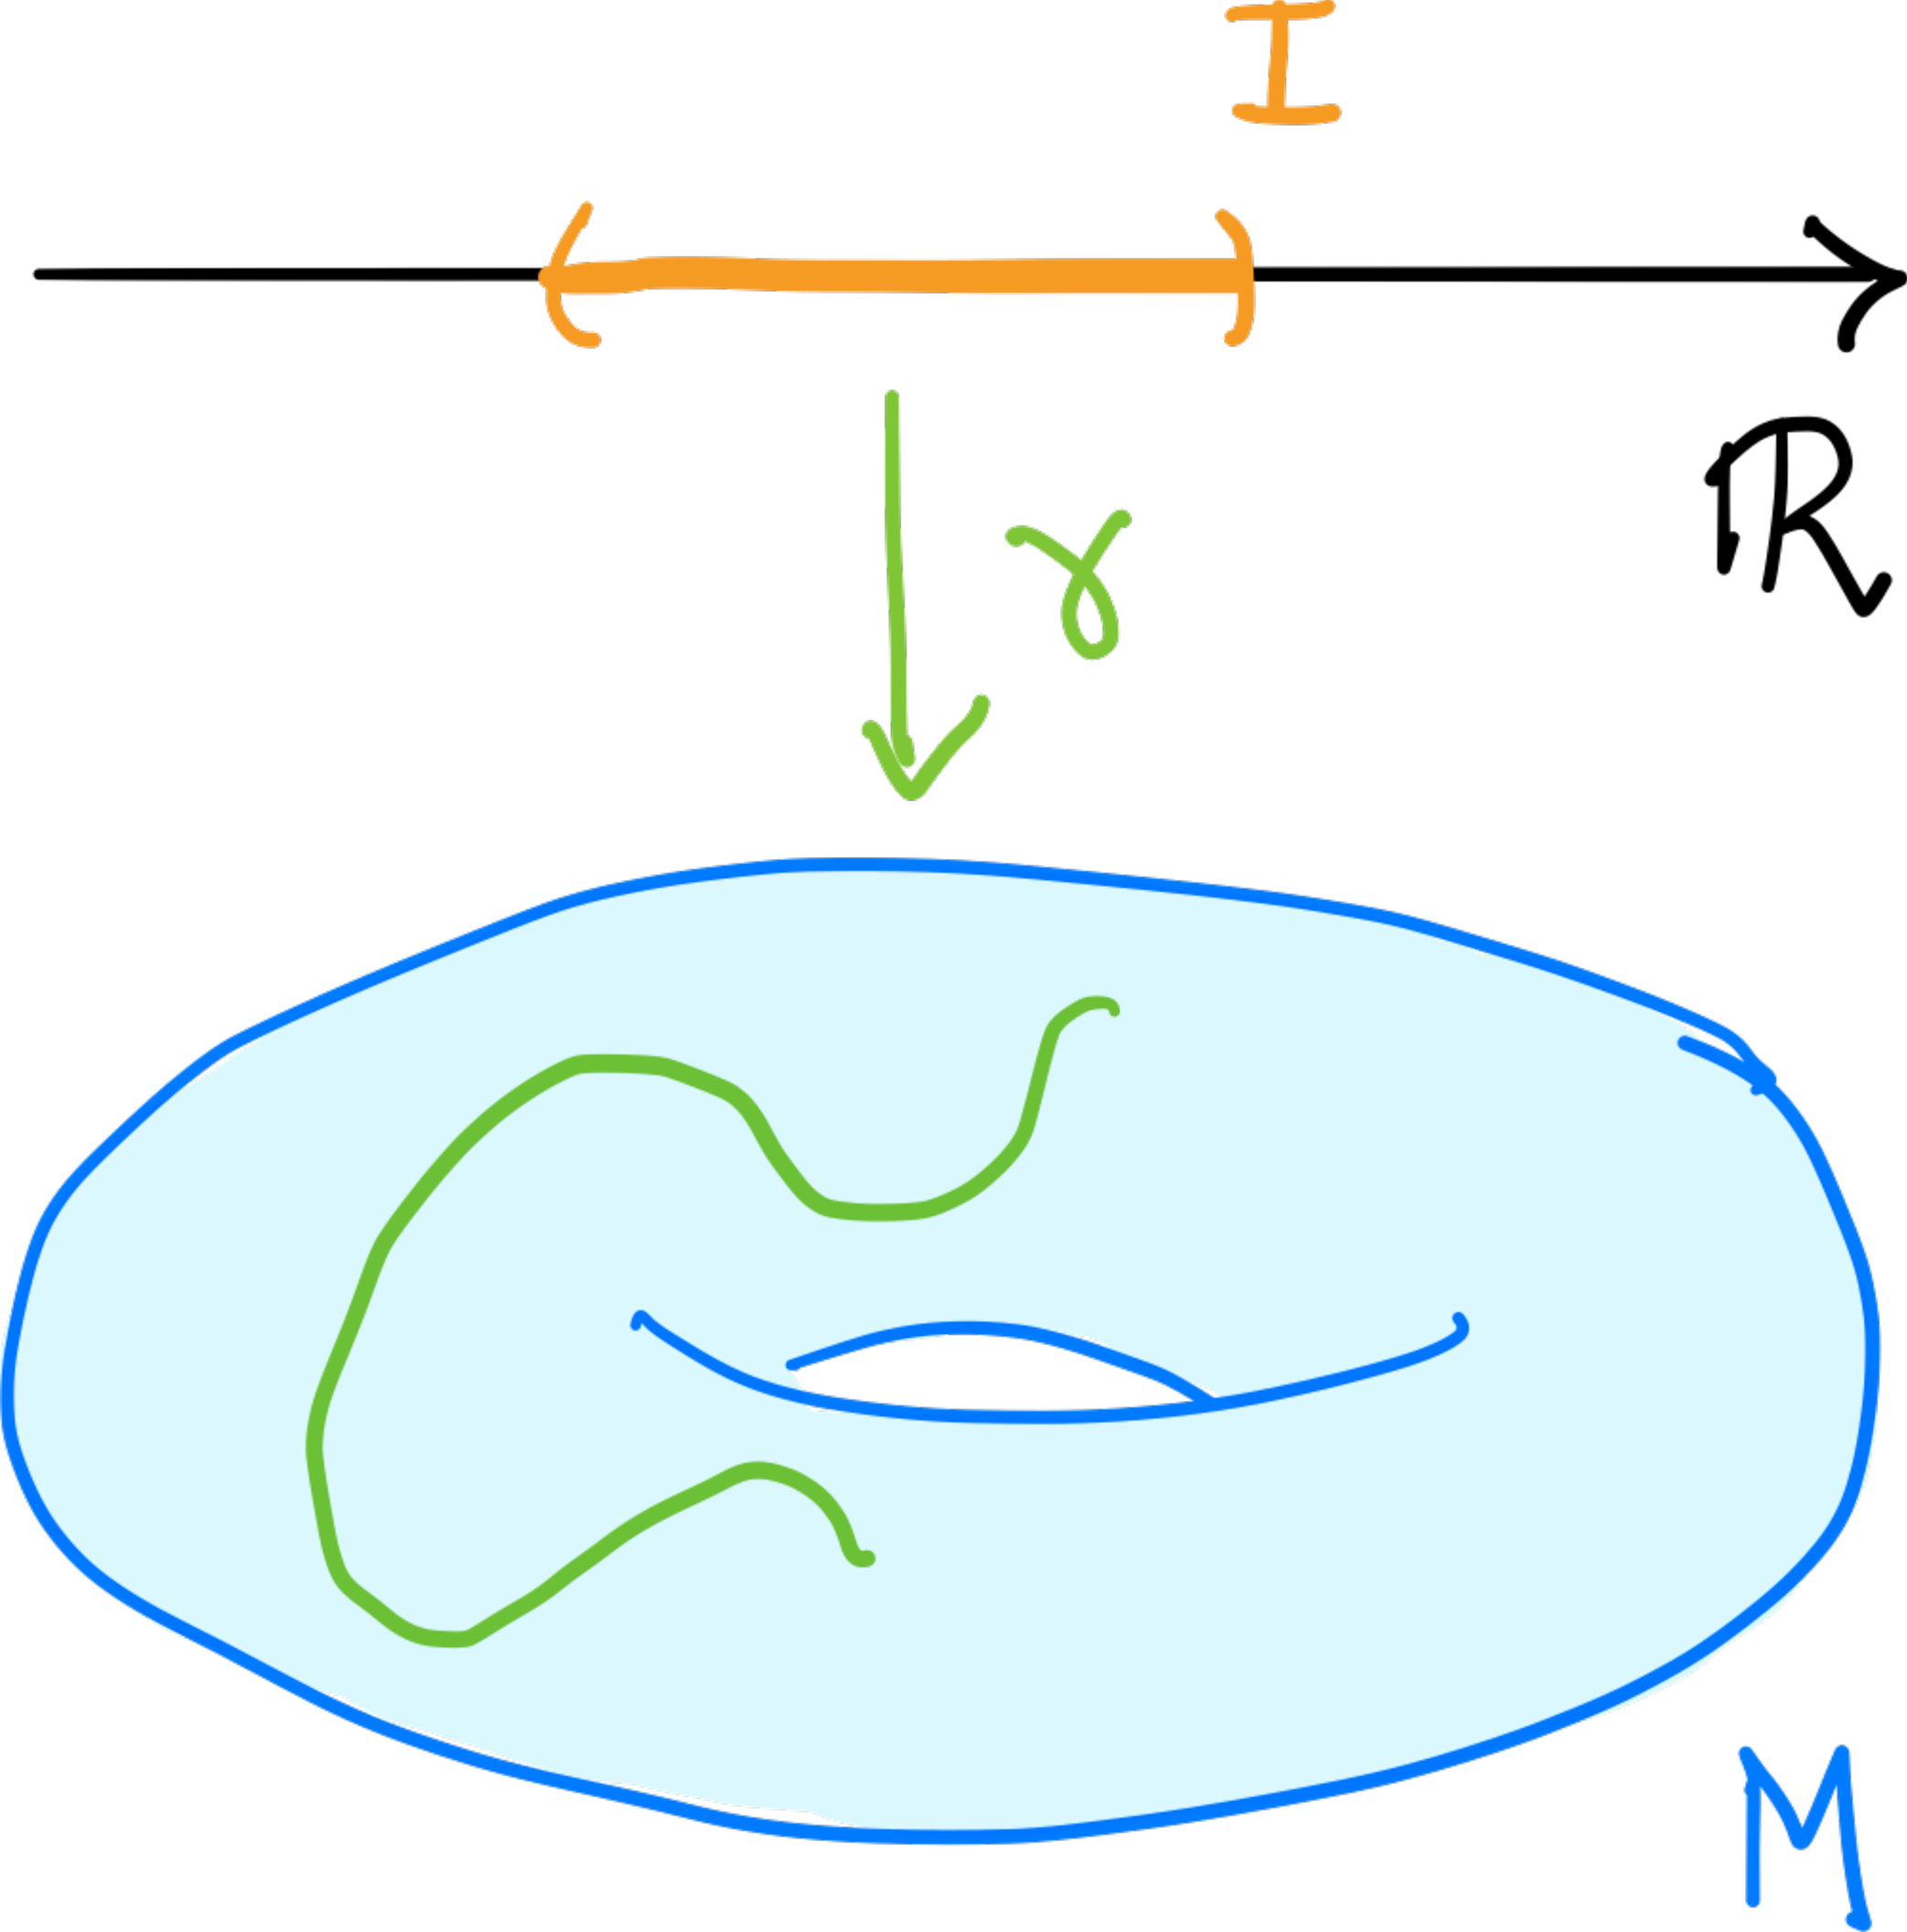
\includegraphics{2_2-curve-on-M.pdf}
\end{marginfigure}

Fix $t\in(a,b)$. 
A priori we have two different ways to define the \emph{velocity vector of $\gamma$ at a time $t$}, that is, an element $\gamma'(t) \in T_{\gamma(t)}M$:
\begin{enumerate}[(i)]
  \item We can define a derivation on $C^\infty(M)$ at $\gamma(t)$ by setting
  \begin{equation}\label{eq:tg_curve_der}
    \gamma'(t) (f) := (f\circ\gamma)'(t), \quad f\in C^\infty(M).
  \end{equation}
  \begin{exercise}
    Show that this is indeed a derivation on $C^\infty(M)$.
  \end{exercise}
  \item If we think of $\gamma$ as a smooth map between manifolds, we can define the tangent vector via the differential $d\gamma_t$:
  \begin{equation}\label{eq:tg_curve_diff}
    \gamma'(t):= d\gamma_t\left(\frac{\partial}{\partial t}\Big|_t\right) \in T_{\gamma(t)}M.
  \end{equation}
\end{enumerate}

Do these definition agree?
One way to check is to pick a chart $\varphi: U \to \varphi(U)$ in a neighbourhood of $\gamma(t)$, and compare the expressions in local coordinates. Let $(x^i)$ denote the coordinates of $\varphi$ and define the curves $\gamma^i := x^i \circ \gamma : I\to\R$.
Let's focus on~\eqref{eq:tg_curve_der}. By definition, $\gamma'(t)(x^i) = (x^i\circ\gamma)'(t) = (\gamma^i)'(t)$, therefore by Proposition~\ref{prop:basis_TpM} we get
\begin{equation}\label{eq:tg_curve_vec}
  \gamma'(t) = %\sum_{i=1}^m
    \gamma'(t)(x^i) \frac{\partial}{\partial x^i}\Big|_{\gamma(t)}.
\end{equation}
\begin{exercise}
  Show that applying Proposition~\ref{prop:DiffCoords} to~\eqref{eq:tg_curve_diff} leads to the same formula as~\eqref{eq:tg_curve_vec}.
\end{exercise}

\begin{figure*}[htp]
  \centering
  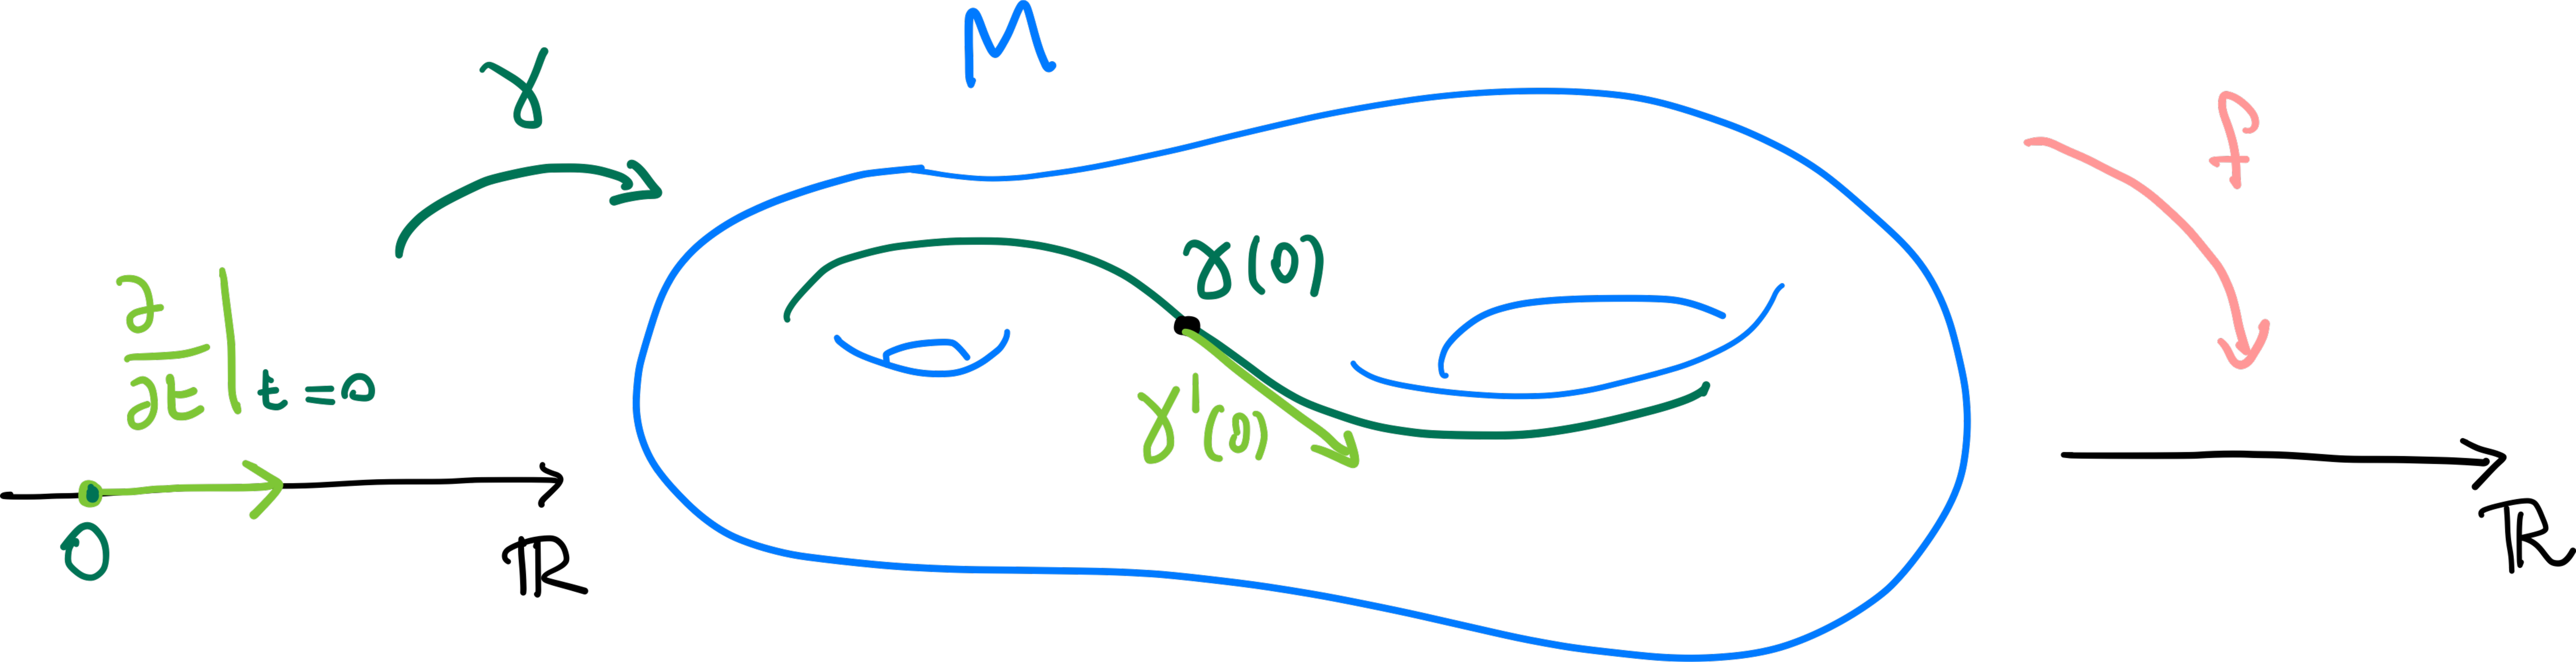
\includegraphics{2_5-v_cur_full.pdf}
  \caption{The velocity of a curve}
  \label{fig:2_5-v_cur_full}
\end{figure*}

But how can this mapping between curves and tangent vector be well--defined?
Surely, there must be multiple curves with the same speed at a point which differ outside a neighbourhood of the point.

\begin{lemma}\label{lem:equiv_tg_curves}
  Let $M$ be a smooth manifolds and $\gamma, \delta : (-\epsilon, \epsilon) \to M$ two smooth curves with $\gamma(0) = \delta(0)$. Then, $\gamma'(0) = \delta'(0)$ as elements of $T_{\gamma(0)}M$ if and only if for some (and thus any) chart $\varphi:U\to\varphi(U)$, $\gamma(0)\in U$, we have $(\varphi\circ \gamma)'(0) = (\varphi\circ\delta)'(0)$.
\end{lemma}
\begin{proof}
  Let $(x^i)$ denote the coordinates of $\varphi$. The condition $(\varphi\circ \gamma)'(0) = (\varphi\circ\delta)'(0)$ is equivalent as stating that $(\gamma^i)'(0) = (\delta^i)'(0)$, where $\gamma^i = x^i\circ\gamma$ and $\delta^i=x^i\circ\delta$. Then, the claim follows from~\eqref{eq:tg_curve_vec} and the fact that $\left\{\frac{\partial}{\partial x^i}\big|_{\gamma(0)}\right\}$ is a basis of $T_{\gamma(0)}M$.
\end{proof}

This seems to follow a pattern: until now, all the definitions of tangent vectors where in terms of classes of equivalence.
And it would seem reasonable to identify curves that that have the same tangent vector at $0$.
There is still a potential problem, though: we don't yet know if \emph{every} tangent vector can be written as the velocity vector of a curve.

\begin{theorem}
  Let $M$ be a smooth $n$-manifold, let $p\in M$ and let $v\in T_pM$.
  There exists a smooth curve $\gamma: (-\epsilon,\epsilon) \to M$ such that $\gamma'(0) = v$.
\end{theorem}
\begin{proof}
  Let $\varphi:U\to\varphi(U)$ be a chart about $p$ such that $\varphi(p)=0$.
  Let $(x^i)$ denote the coordinates of $\varphi$, as usual, and assume that
  \begin{equation}
    v = \sum_{i=1}^n a^i \frac{\partial}{\partial x^i}\Big|_p, \qquad a^i \in\R.
  \end{equation}
  For $\epsilon$ small enough, by continuity the vector $(ta^1, \ldots, ta^n) \in \varphi(U)$ for all $|t|<\epsilon$. Therefore, the curve
  \begin{equation}
    \gamma: (-\epsilon, \epsilon) \to M, \quad \gamma(t):=\varphi^{-1}(ta^1, \ldots, ta^n),
  \end{equation}
  is well-defined, smooth, satisfies $\gamma(0) = p$ and, by~\eqref{eq:tg_curve_vec}, $\gamma'(0) = v$.
\end{proof}

\begin{marginfigure}
  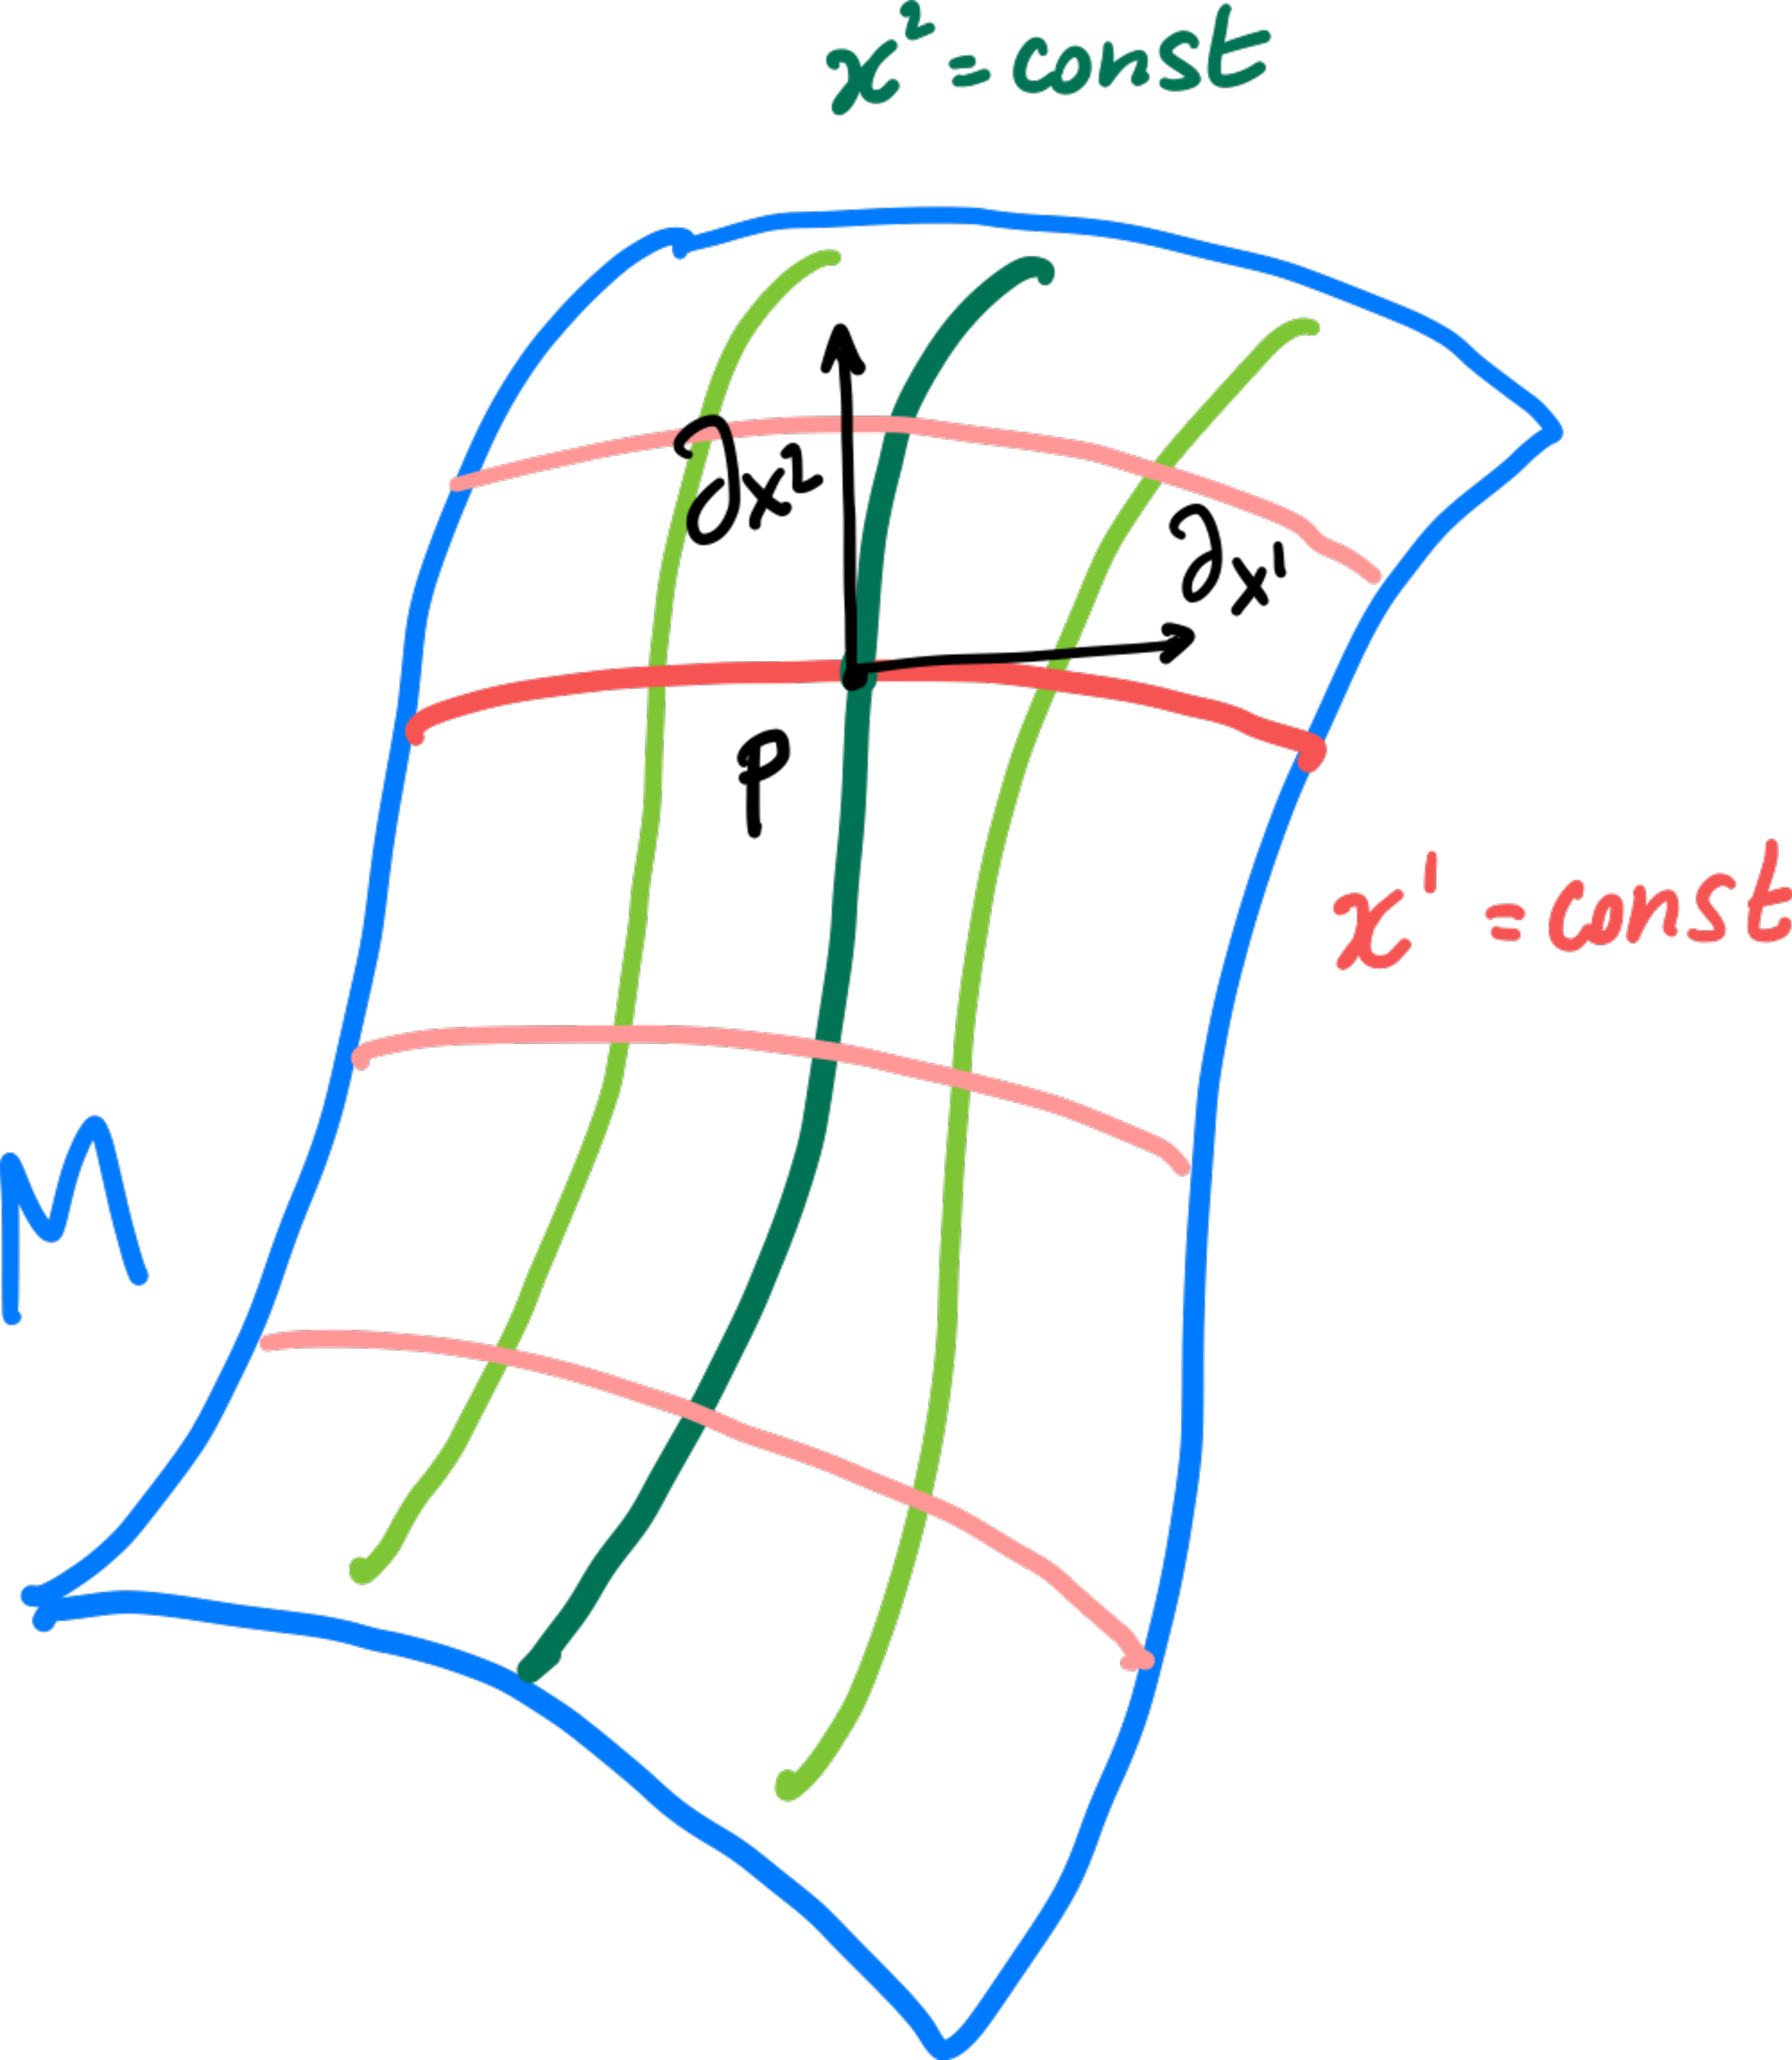
\includegraphics{2_4-v_cur.pdf}
  \caption{With this definition, the coordinate tangent vectors $\partial_{x^i}\in T_p M$ become the tangent vectors defined by the curve \[t \mapsto \varphi^{-1}(x^1(p), \ldots, {x^i(p) + t}, \ldots, x^n(p)).\]}
  \label{fig:2_4-v_cur}
\end{marginfigure}
This means that we can actually give an alternative definition of $T_xM$ in terms of tangents to curves:
\begin{definition}\label{def:tg:ascurvespeed}
  A tangent vector at $p\in M$ is an equivalence class of smooth curves $\gamma:(-\epsilon, \epsilon)\to M$ such that $\gamma(0)=p$, where $\gamma\sim\delta$ if and only if $(\varphi\circ \gamma)'(0) = (\varphi\circ\delta)'(0)$ for some chart $\varphi$ centred about $p$ (see Lemma~\ref{lem:equiv_tg_curves}).
\end{definition}

In fact, it is possible to start the whole tangent space discussion with the above definition. In that case, you would first need to prove Exercise~\ref{exe:vsstruct} and endow $T_pM$ with a vector space structure\footnote{To get the analogue result as Proposition~\ref{prop:basis_TpM}}.

To conclude this part, the next proposition shows that velocity vectors behave well under composition with smooth maps and give us a direct, explicit and effective way to compute differentials.

\begin{proposition}\label{prop:curves_deriv}
  Let $F:M\to N$ b a smooth map between smooth manifolds and $\gamma:I\to M$ a smooth curve in $M$.
  Then
  \begin{equation}
    d F_{\gamma(t)} (\gamma'(t)) = (F\circ\gamma)'(t).
  \end{equation}
\end{proposition}
\begin{proof}
  We are going to use~\eqref{eq:tg_curve_diff} as definition of $\gamma'(t)$.
  Applying the chain rule we obtain:
  \begin{align}
    d F_{\gamma(t)} (\gamma'(t))
    &= d F_{\gamma(t)} \circ d\gamma_t\left(\frac{\partial}{\partial t}\Big|_t\right) \\
    &= d (F\circ\gamma)_t \left(\frac{\partial}{\partial t}\Big|_t\right) \\
    &= (F\circ\gamma)'(t).
  \end{align}
\end{proof}

\begin{exercise}
  Give an alternative proof of Proposition~\ref{prop:curves_deriv} using~\eqref{eq:tg_curve_der} as definition for $\gamma'(t)$.\\
 \textit{\small Hint: use the definitions to rewrite the formula in different ways.}
\end{exercise}

\section{The tangent bundle}\label{sec:tangentbundle}

Instead of working separately with the various tangent spaces, we can ``glue'' them together into a big manifold.

\begin{marginfigure}
  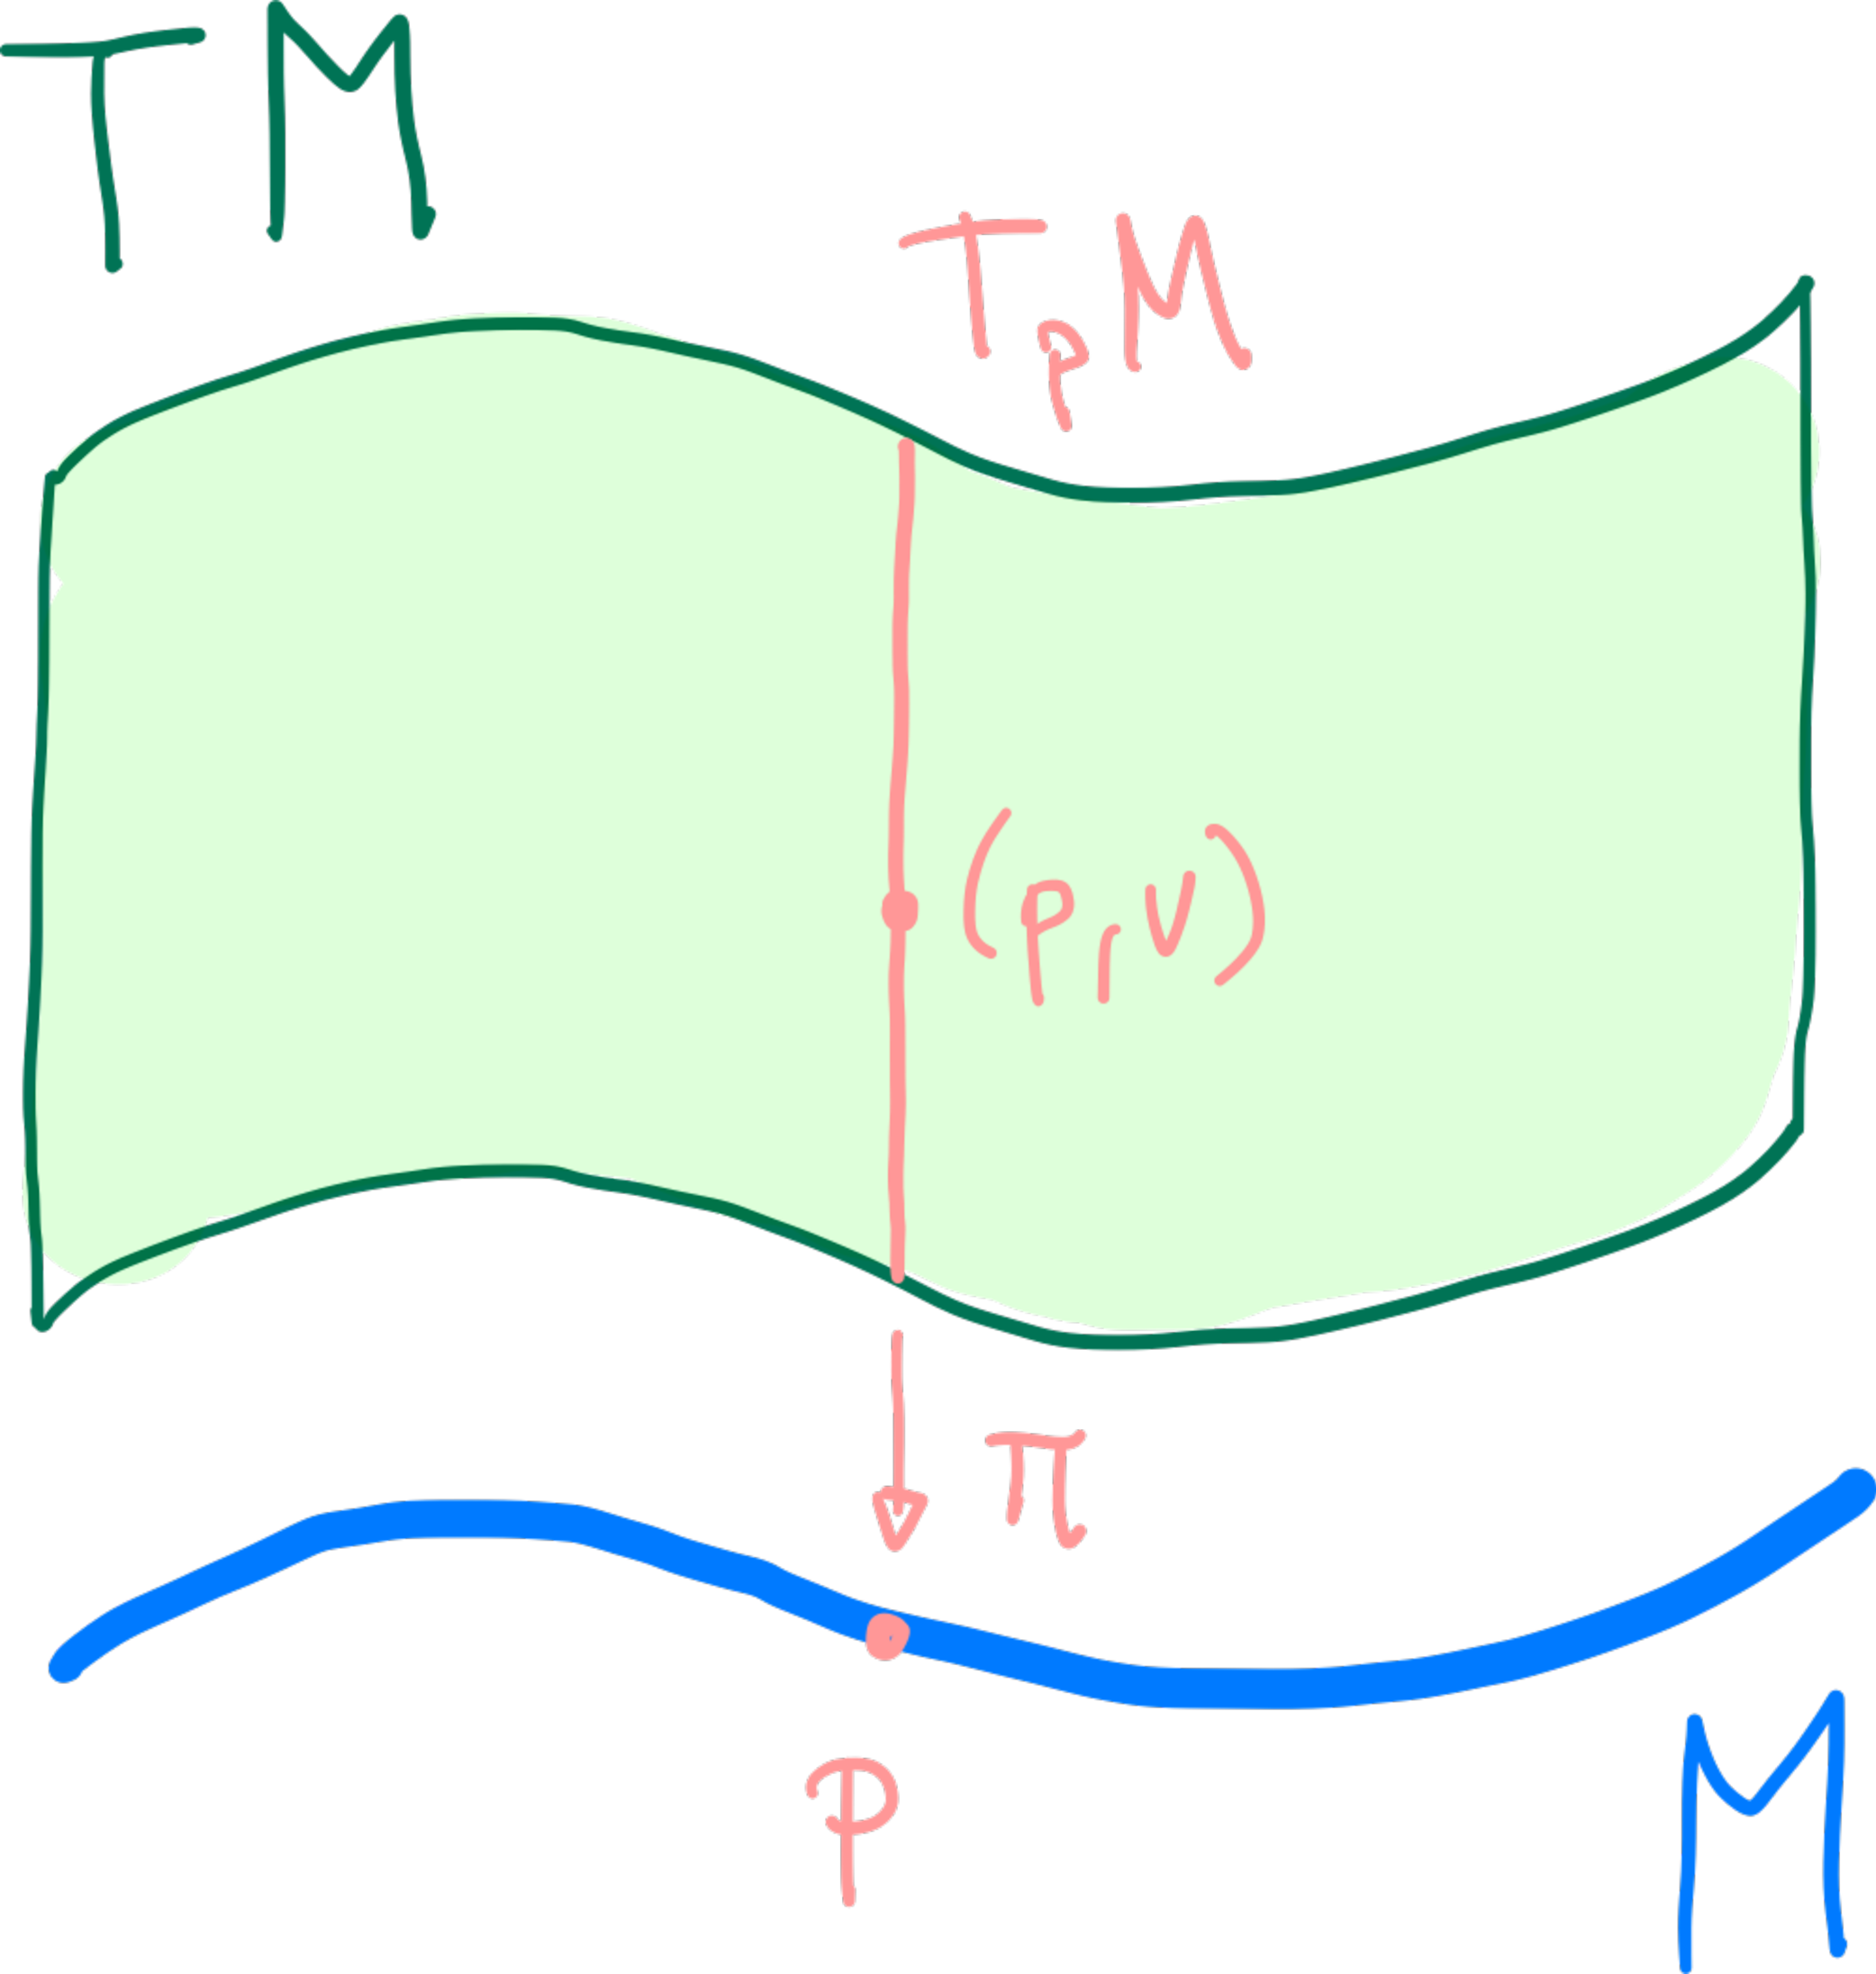
\includegraphics{2_6-tg_bdl_proj.pdf}
\end{marginfigure}
\begin{definition}
  The \emph{tangent bundle} $TM$ of $M$ is the disjoint union of the tangent spaces
  \begin{equation}
    TM := \bigsqcup_{p\in M}\left(\{p\}\times T_pM\right)
       = \{(p,v) \;\mid\; p\in M,\, v\in T_pM\}.
  \end{equation}  
\end{definition}

Elements in $TM$ are pairs\footnote{We will often abuse notation and identify $T_pM$ with with its image under the canonical injection $v\mapsto(p,v)$ and use interchangeably any of the notations $v$, $v_p$ or $(p,v)$ for a vector in $T_pM$ (depending on how much emphasis we need to put on the base point).} $(p,v)$ of a \emph{base point} $p\in M$ and a \emph{tangent vector} $v\in T_pM$.

To the tangent bundle we associate a surjective map $\pi:TM \to M$, the \emph{projection (onto the base)}, which sends each vector in a tangent space to the point at which it is tangent, that is, $\pi(p,v) = p$.
The second component of the pre-image $\pi^{-1}(\{p\}) = \{p\}\times T_pM$, that is $T_pM$ itself, is called the \emph{fibre} over $p\in M$.
We will come back to this later on once we talk about vector bundles.

\begin{example}
  Let $M\subset \R^n$ be an an open set.
  We can identify $TM$ in a natural way with $M\times\R^n$.
  Since $M\times\R^n \subset \R^{2n}$ and thus is a manifold, we can equip the tangent bundle $TM$ with the structure of a manifold induced by this identification.
\end{example}

As it turns out, this is a particular instance of a more general fact.

\begin{theorem}\label{thm:tgbdlsmoothmfld}
  Let $M$ be a smooth $n$-manifold.
  The smooth structure on $M$ naturally\footnote{In the sense that its definition does not require to make any arbitrary choices.} induces a smooth structure on $TM$, making $TM$ into a smooth manifold of dimension $2n$.
  Moreover, the map $\pi: TM \to M$ is smooth.
\end{theorem}
\begin{proof}
  \marginnote[1em]{In this proof you can see instances of a typical abuse of notation: in the expressions $\widetilde x^i(x)$ we think of the $\widetilde x^i$ as coordinate functions but we think of the $x$ as representing a point in $\varphi(U\cap V)$.}
  \newthought{Step 1: extending charts from $M$ to $TM$.}
  Given a chart $(U,\varphi)$ about $p\in M$, the preimage $\pi^{-1}(U) \subset TM$ is the set of all tangent vectors to $M$ at points of $U$.
  If $(x^i)$ denotes the coordinate functions of $\varphi$, we can define a map $\widetilde\varphi : \pi^{-1}(U) \to \varphi(U)\times\R^n \subset \R^{2n}$ by
  \marginnote{Keep in mind that \begin{equation}\nonumber
    \pi^{-1}(U)= TU = \bigsqcup T_p U \subset \bigsqcup T_p M=TM.
  \end{equation}}
  \begin{align}\label{eq:nat_coords}
    \widetilde\varphi\left(v^i \frac{\partial}{\partial x^i}\Big|_p\right) := \left(x^1(p), \ldots, x^n(p), v^1, \ldots, v^n\right).
  \end{align}
  Since $\widetilde\varphi$ can be explicitly inverted as $\widetilde\varphi^{-1}\left(x^1, \ldots, x^n, v^1, \ldots, v^n\right) = v^i \frac{\partial}{\partial x^i}\Big|_{\varphi^{-1}(x)}$, it defines a bijection onto its image.

  \newthought{Step2: compatibility of the extended charts.}
  Suppose we have two smooth charts $(U,\varphi)$, $(V,\psi)$ for $M$ with the respective local coordinates $(x^i)$ and $(y^i)$.
  Let $(\pi^{-1}(U),\widetilde\varphi)$, $(\pi^{-1}(V),\widetilde\psi)$ be their extension\footnote{These are called \emph{bundle charts}.} to $TM$ as in the previous step.
  By construction\footnote{They are both homeomorphisms.}, both $\widetilde\varphi(\pi^{-1}(U)\cap\pi^{-1}(V)) = \varphi(U\cap V)\times\R^n$ and $\widetilde\psi(\pi^{-1}(U)\cap\pi^{-1}(V)) = \psi(U\cap V)\times\R^n$ are open in $\R^{2n}$.
  Moreover, we can take advantage of Remark~\ref{rmk:chg_coords} to write explicitly the transition map  $\widetilde\psi\circ\widetilde\varphi^{-1}: \varphi(U\cap V)\times\R^n \to \psi(U\cap V)\times\R^n$ as
  \begin{align}
    \widetilde\psi\circ&\widetilde\varphi^{-1}\left(x^1, \ldots, x^n, v^1, \ldots, v^n\right) \\
    &=\left(y^1(p),\ldots, y^n(p), \frac{\partial y^1}{\partial x^j}(p) v^j, \ldots, \frac{\partial y^n}{\partial x^j}(p) v^j\right),
  \end{align}
  where $p = \phi^{-1}(x)$, which is clearly smooth.
  
  \begin{figure*}[htp]
    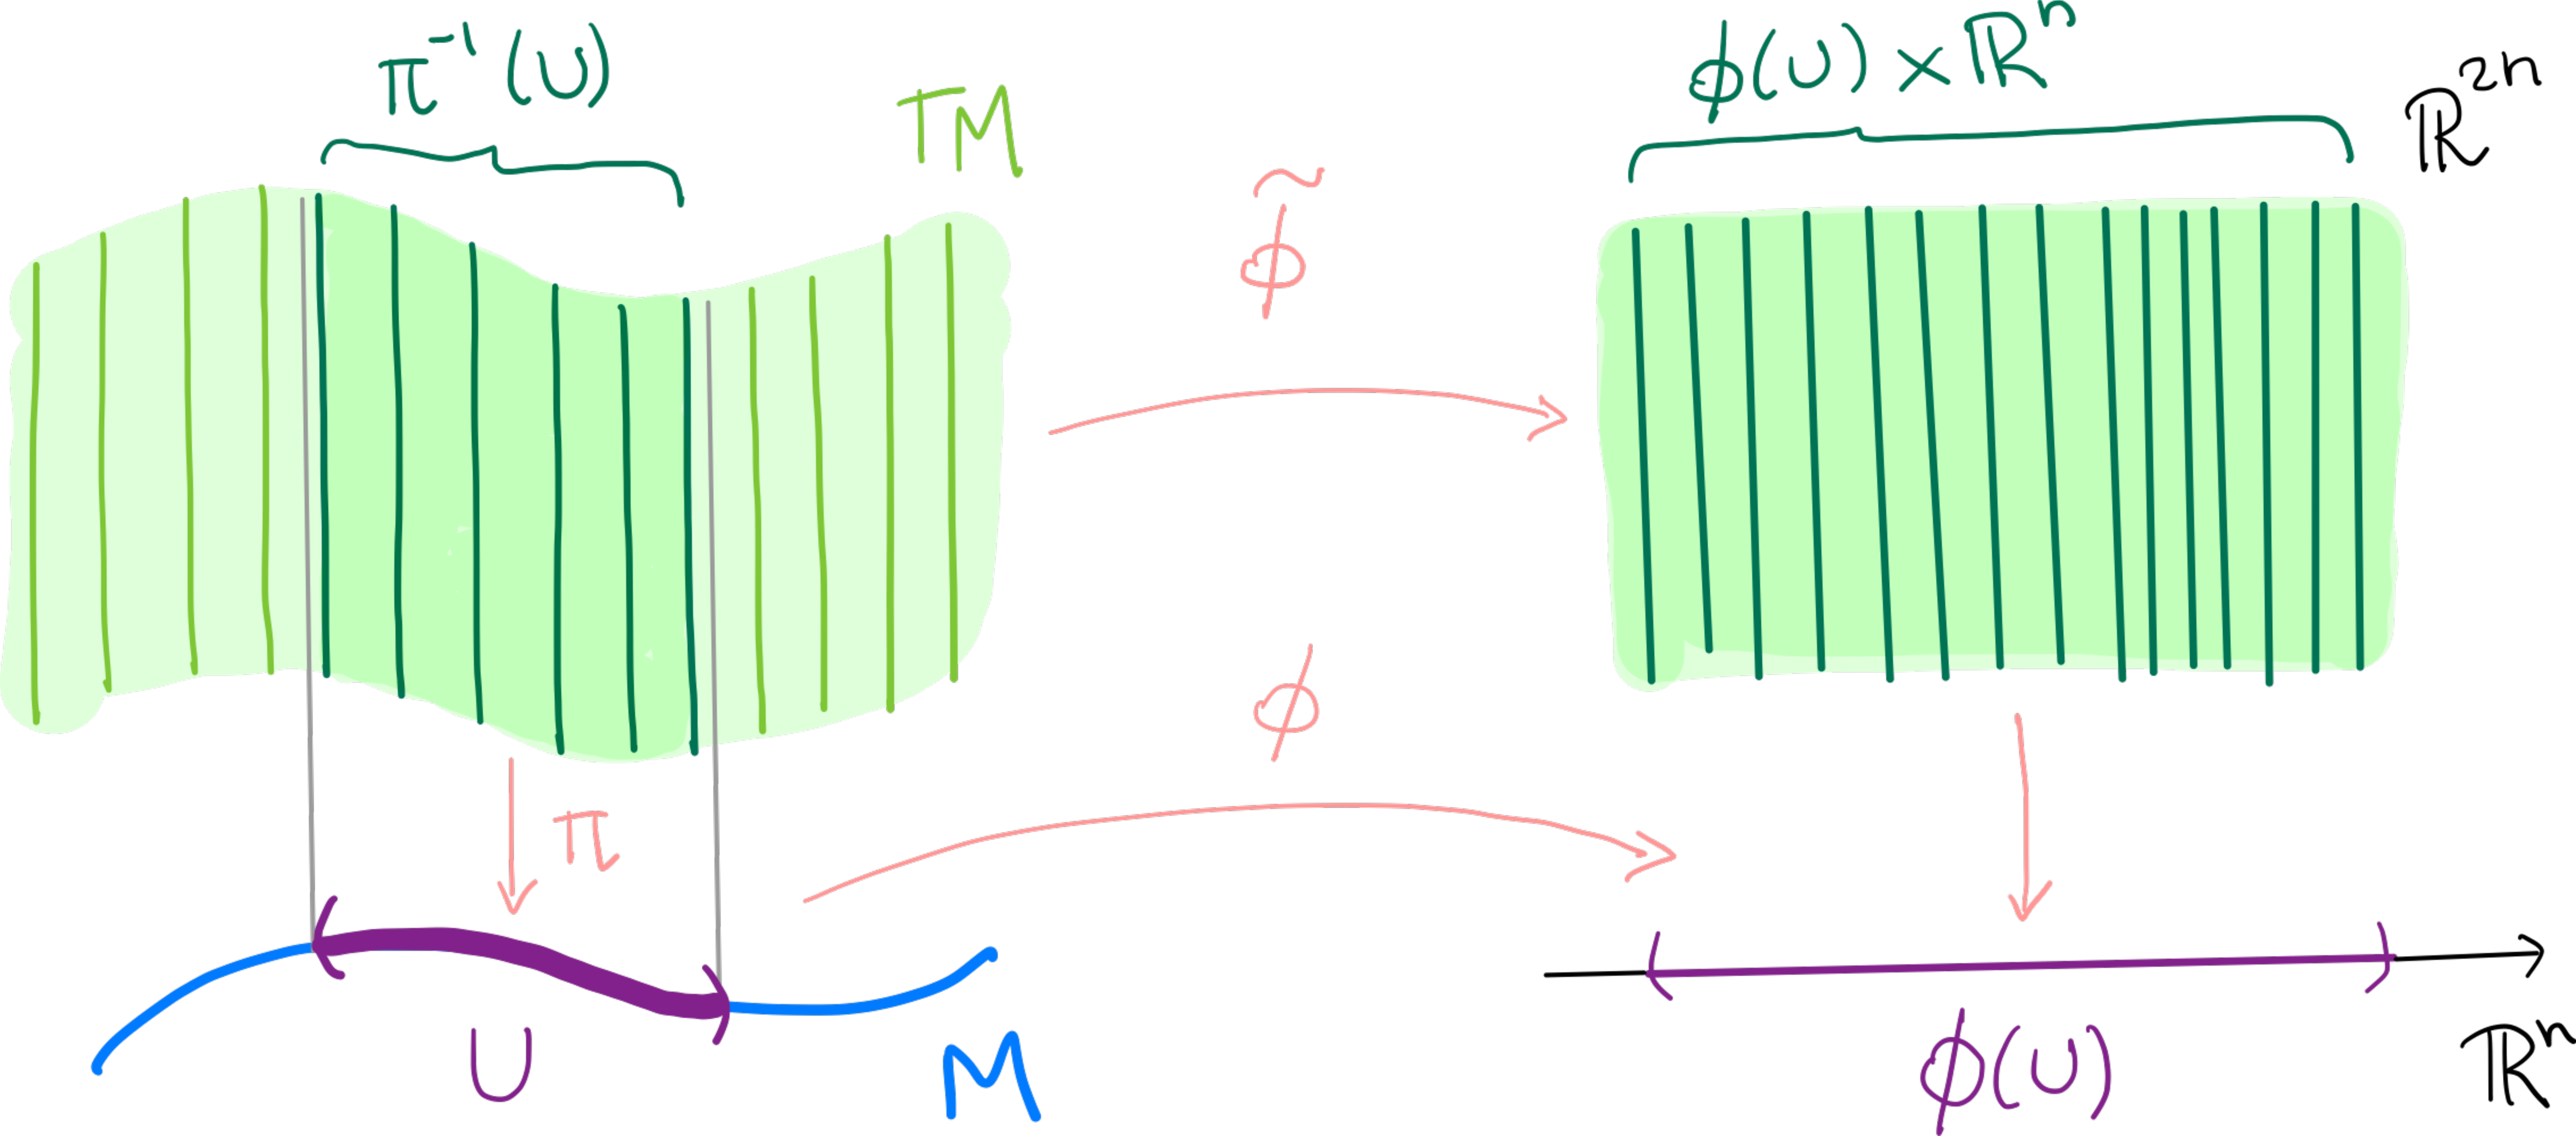
\includegraphics{2_7-tg_bdl_coord.pdf}
    \caption{Coordinates for the tangent bundle}
  \end{figure*}
  
  \newthought{Step3: $TM$ is a manifold.}
  With the procedure delineated above, a countable smooth atlas $\{(U_i, \varphi_i)\}$ of $M$ induces a countable atlas $\{(\pi^{-1}(U_i), \widetilde\varphi_i)\}$ of $TM$.
  First of all, $\{(\pi^{-1}(U_i)\}$ provides a countable covering of $TM$.
  We need to show that the topology induced by those charts is Hausdorff and second countable.
  
  Let $(p_1, v_1), (p_2, v_2) \in TM$ be different points: either $p_1\neq p_2$, or $p_1 = p_2$ and $v_1 \neq v_2$.
  \begin{itemize}
    \item In the first case, there are disjoint open sets $V_1, V_2 \subset U_i$ (for some $i$) containing respectively $p_1$ and $p_2$.
    Then $\widetilde\varphi_i^{-1}(\varphi_i(V_1)\times\R^n)$ and $\widetilde\varphi_i^{-1}(\varphi_i(V_2)\times\R^n)$ are disjoint open sets containing respectively $(p_1, v_1)$ and $(p_2, v_2)$.
    \item In the second case, $p=p_1=p_2$ but there are disjoint open sets $V_1,V_2\subset \R^n$ containing $v_1$ and $v_2$ respectively;
    again, the preimages $\widetilde\varphi_i^{-1}(\varphi_i(U_i)\times V_1)$ and $\widetilde\varphi_i^{-1}(\varphi_i(U_2)\times V_2)$ (for some $i$ such that $p\in U_i$) are disjoint open sets containing respectively $(p_1, v_1)$ and $(p_2, v_2)$.
  \end{itemize}

  The countable basis $\{U_j\}$ is a countable basis for the topology of $M$ (which is second countable), taking a countable basis $\{W_k\}$ for the topology of $\R^n$, we can define a countable basis for $TM$ as $\{\widetilde\varphi^{-1}((U_i\cap U_j)\times W_k)\}$.
  The charts defined above make $TM$ automatically euclidean of dimension $2n$.

  \begin{exercise}
    This part of the proof seems unnecessarily detailed.
    Can you simplify it using Lemma~\ref{lem:manifold_chart}?
  \end{exercise}

  \newthought{Step4: $\pi$ is smooth.} With respect to the charts $(U,\varphi)$ for $M$ and $(\pi^{-1}(U), \widetilde\varphi)$ for $TM$, the coordinate representation of $\pi$ is $\pi(x,v) = x$.
\end{proof}

The coordinates $(x^i, v^i)$ defined by~\eqref{eq:nat_coords} are called \emph{natural (or canonical) coordinates}.

\begin{exercise}
  Let $f:M\to N$ be a smooth map between smooth manifolds.
  Show that its differential $df: TM \to TN$ is a smooth map between smooth manifolds (the respective tangent bundles).\\
  \textit{\small Hint: use the natural differentiable structure on the tangent bundle described above and the definition of smooth map.}
\end{exercise}

\begin{remark}
  In classical mechanics, the configuration space is usually a manifold $M$.
  The tangent bundle $TM$ corresponds to the state space, that is, the space of configurations and velocities. In symbols $x=(q,v)$ is a pair of a configuration $q = \pi(x)$ and a velocity $v\in T_q M$.
  It turns out that the Lagrangian is a smooth function on $TM$.
\end{remark}

\section{Vector bundles}\label{sec:vectorbundle}

What we have seen here is our first example of vector bundle, which is just a way to call a vector space depending continuously (or smoothly) on some parameters, for example points on a manifold.

\begin{definition}\label{def:vector_bundle}
  A \emph{vector bundle of rank $r$} on a manifold $M$ is a manifold $E$ together with a smooth surjective map $\pi : E \to M$ such that, for all $p\in M$, the following properties hold:
  \begin{enumerate}[(i)]
    \item the \emph{fibre over $p$}, $E_p := \pi^{-1}(p)$, has the structure of vector space of dimension $r$;
    \item there is a neighbourhood $U\subset M$ of $p$ and a diffeomorphism $\varphi: \pi^{-1}(U) \to U \times \R^r$ such that
    \begin{enumerate}
      \item $\pi_1 \circ \varphi = \pi$ where $\pi_1: U\times\R^r\to U$ is the projection on the first factor,
      \item for all $q\in U$, $\varphi\big|_{E_q} : E_q \to \{q\}\times \R^r$ is an isomorphism of vector spaces.
    \end{enumerate}
  \end{enumerate}

  The space $E$ is called the \emph{total space}, the manifold $M$ is the \emph{base space}, $\pi$ its projection and each of the maps $\varphi$ is called \emph{local trivialisation}.

  If there exists a trivialisation defined on the whole manifold, that is a map $\varphi: M \to M\times \R^r$, such map is called \emph{global trivialisation} and the vector bundle is said to be \emph{trivialisable}.
\end{definition}

\begin{example}
  \begin{itemize}
    \item A simple example of vector bundle of rank $r$ over a manifold $M$ is the product space $E = M\times \R^r$ itself with the projection on the first component $\pi_1: E\to M$.
    In this case the bundle is clearly trivialisable.
    \item The tangent bundle $TM$ with its projection to the base $\pi:TM\to M$ is a vector bundle.
    In this case the fibres are the tangent spaces $\pi^{-1}(p) = T_pM$. 
    If the tangent bundle of a manifold is trivalisable, then its base manifold is said to be \emph{parallelisable}.
    \item If $\pi_i: E_i\to M_i$, $i=1,2$, are vector bundles, then $\pi = (\pi_1, \pi_2): E_1\times E_2 \to M_1\times M_2$ is another vector bundle whose fibres are the product of the fibres of the two original bundles.
    A particular example of this is the tangent bundle $T(M_1\times M_2)$, which is diffeomorphic to $TM_1 \times TM_2$.
    \item Other examples will appear throughout the course.
  \end{itemize}
\end{example}

\begin{exercise}
  Show that $\dim(E) = \dim(M) + r$.
\end{exercise}

\begin{exercise}
  Show that if $\pi:E\to M$ is a vector bundle and $U\subset M$ is an open set, then $\pi\big|_{\pi^{-1}(U)}: \pi^{-1}(U) \to U$ is a vector bundle of the same rank.
\end{exercise}

\begin{example}
  Let $\pi:E \to M$ be a vector bundle of rank $r$.
  Assume that $E$ itself is the base space of another vector bundle $\pi_1: E_1\to E$ of rank $s$.
  Then $\pi\circ\pi_1: E_1 \to M$ is a vector bundle of rank $r+s$ called the \emph{composite bundle}. Indeed, if $\varphi:\pi^{-1}(U)\to U\times\R^r$ is a bundle diffeomorphism for $E$ over $U\subset M$ and $\varphi_1:\pi_1^{-1}(U_1)\to U_1\times\R^s$ is a bundle diffeomorphism for $E_1$ over $U_1\subset E$ such that $V := \pi(U_1)\cap U\neq \emptyset$, then
  \begin{equation}
    \Psi:=(\varphi\circ\pi_1, \varphi_1): (\pi\circ\pi_1)^{-1}(V)\to (U\times\R^r)\times (U_1\times\R^s)
  \end{equation}
  is a bundle diffeomorphism for $\pi\circ\pi_1$ over $W$.

  A particular example of this is the tangent bundle of the tangent bundle: if $M$ is a $n$-manifold, its tangent bundle $TM$ is a $2n$-manifold, and its tangent bundle $T(TM)$ is a vector bundle over $M$ of rank $3n$.
\end{example}

To compare vector bundles is useful to define the following concept.
\begin{definition}
  A \emph{isomorphims} between two vector bundles $\pi_i: E_i \to M$, $i=1,2$, over the same base space $M$ is a homeomorphism $h:E_1 \to E_2$ which maps every fiber $\pi_1^{-1}(p)$ to the corresponding fiber $\pi_2^{-1}(p)$ by a linear isomorphism.
\end{definition}

Since an isomorphism preserves all the structure of a vector bundle, isomorphic bundles are often regarded as the same.

\begin{marginfigure}[-30em]
  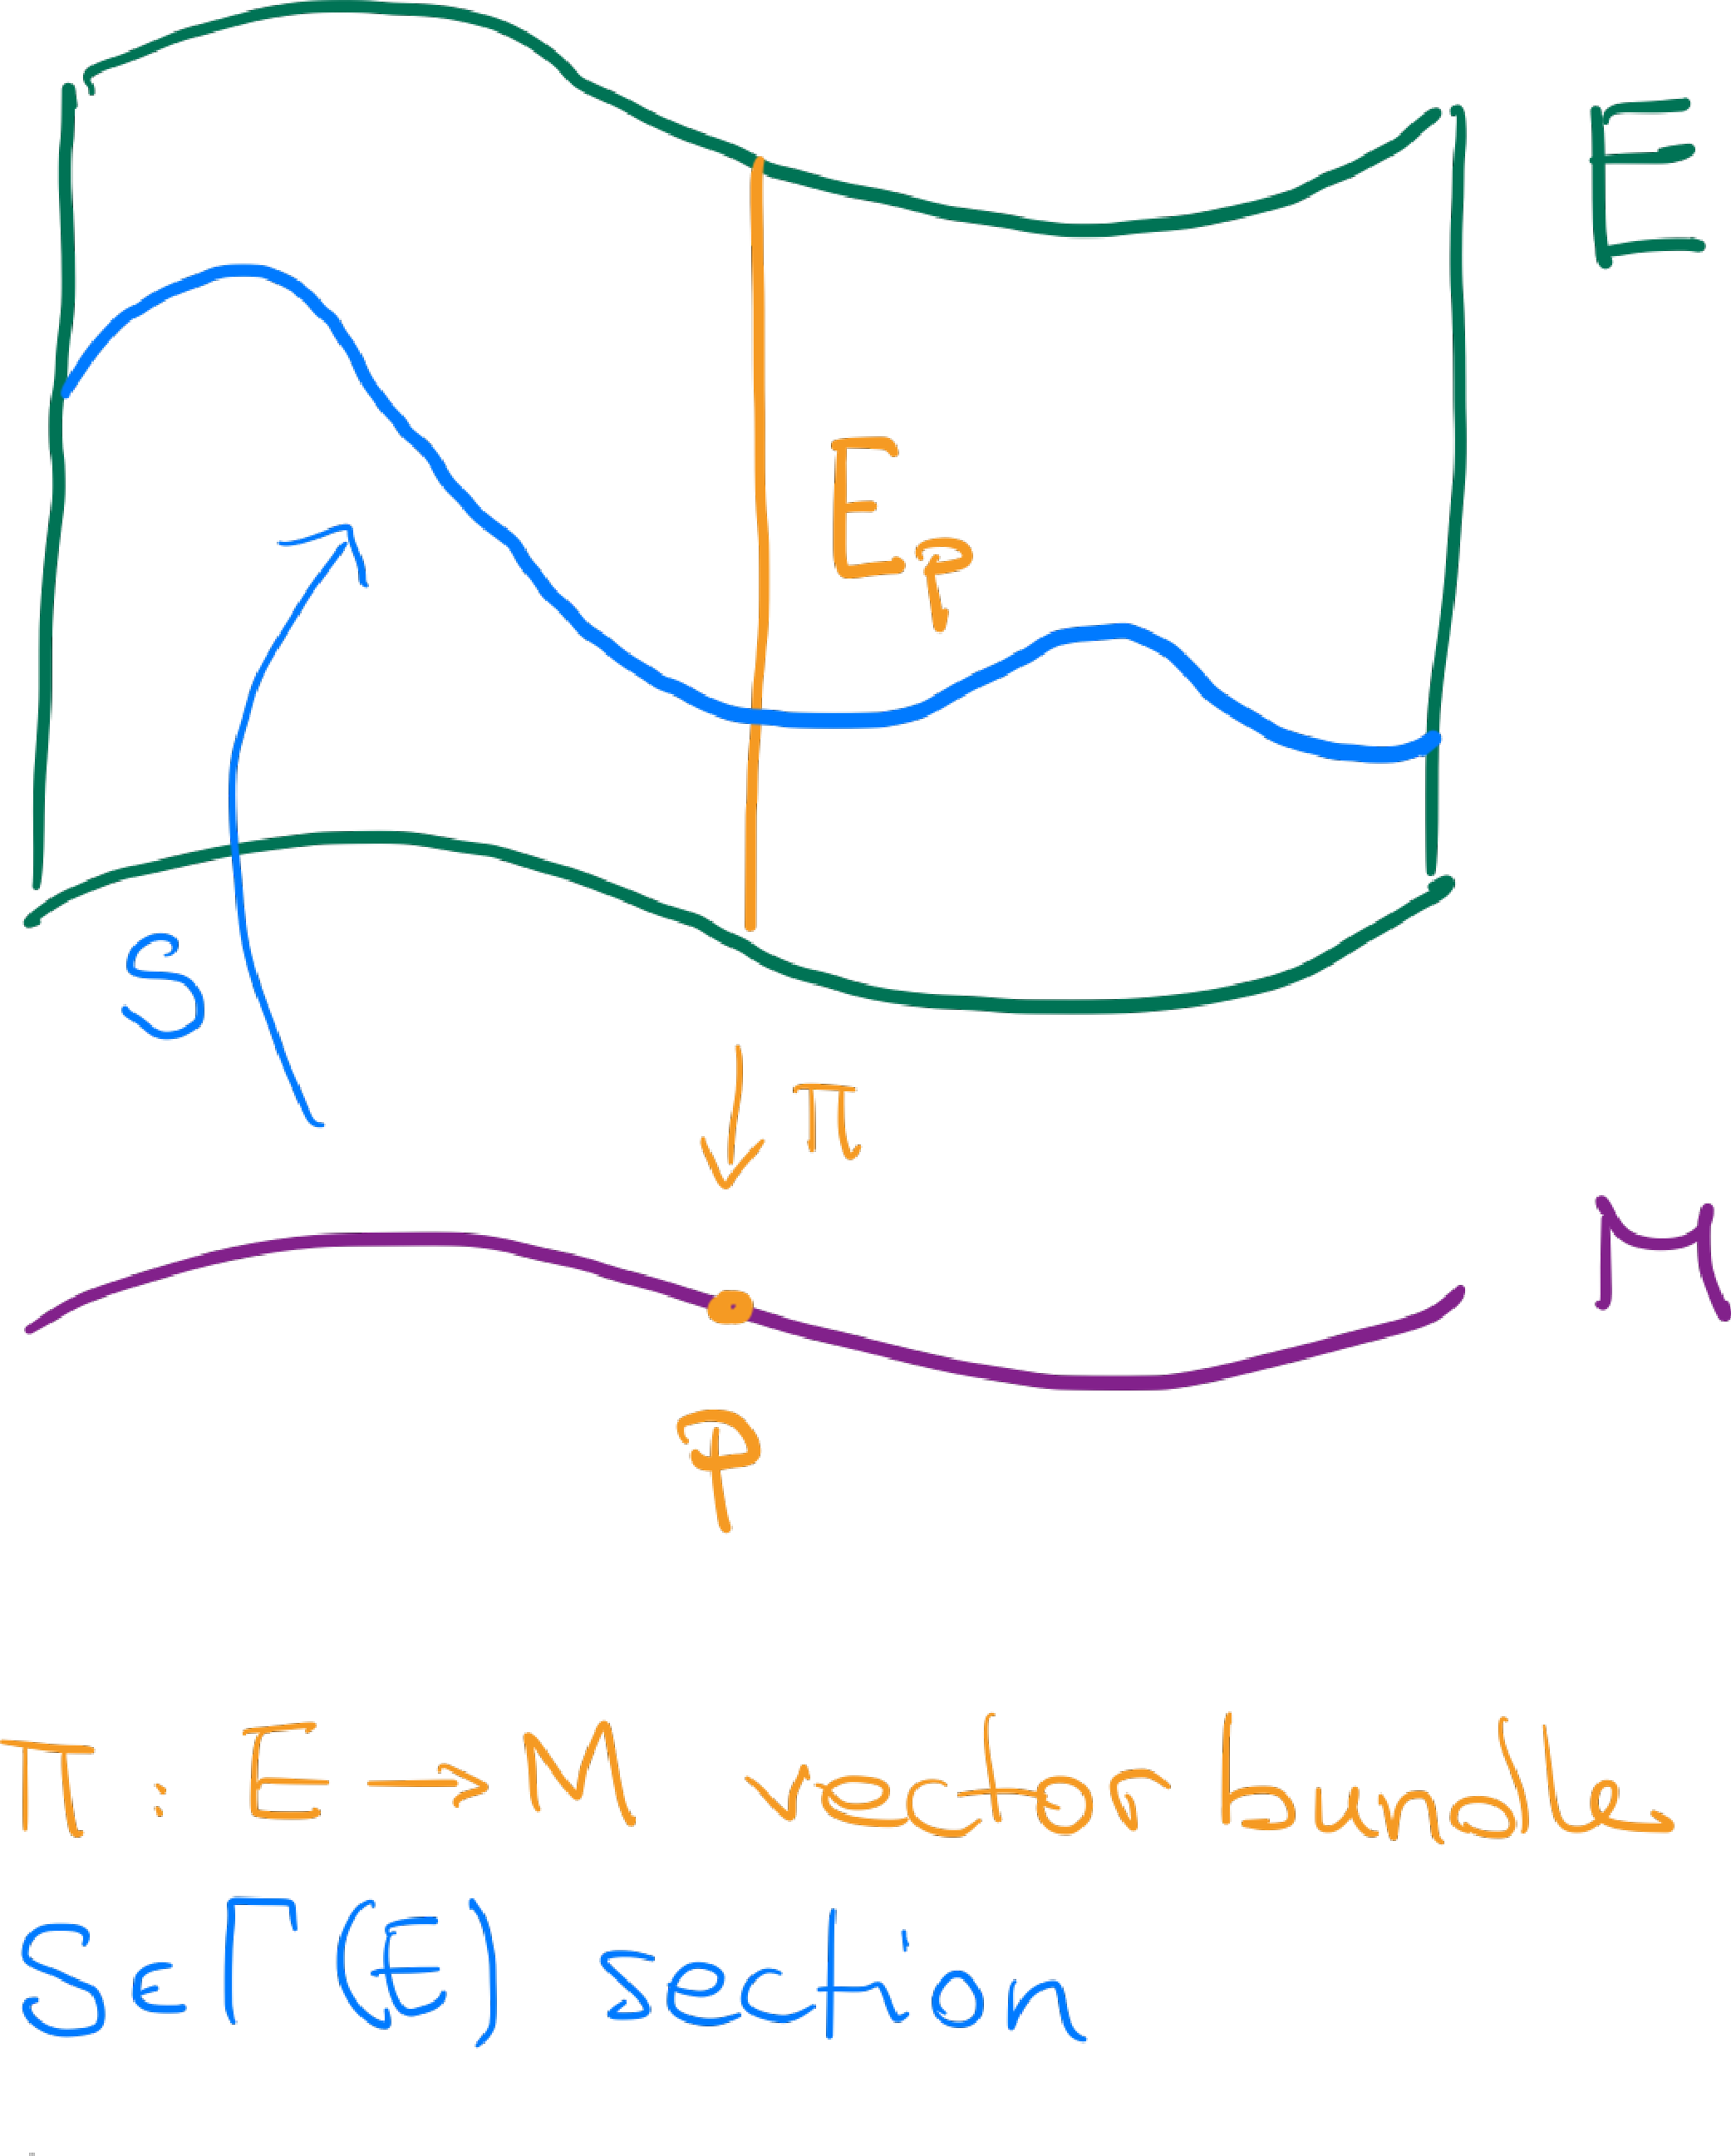
\includegraphics{2_7-bdl_section.pdf}
  \caption{A useful mnemonic to remember what is a section, is to imagine it as a cross-section of the bundle.}
\end{marginfigure}

\begin{definition}
  A \emph{section} of a vector bundle $\pi:E \to M$ is a smooth map $S:M \to E$ such that $\pi\circ S = \id_M$. We denote the set of all sections of $E$ by $\Gamma(E)$.
  
  If, in the definition, $M$ is replaced by $U\subset M$, the section is called \emph{local section}. The set of local sections on $U\subset M$ is denoted $\Gamma(E|_U)$.
\end{definition}

\begin{example}
  If $E = M\times \R^r$, $M\subset\R^n$, then for any smooth map $F: M\to\R^r$ we have a section $S\in\Gamma(E)$ defined by $S(p) = (p, F(p))$. This is a classical euclidean vector field: a map that associates vectors to points.
  \begin{marginfigure}
    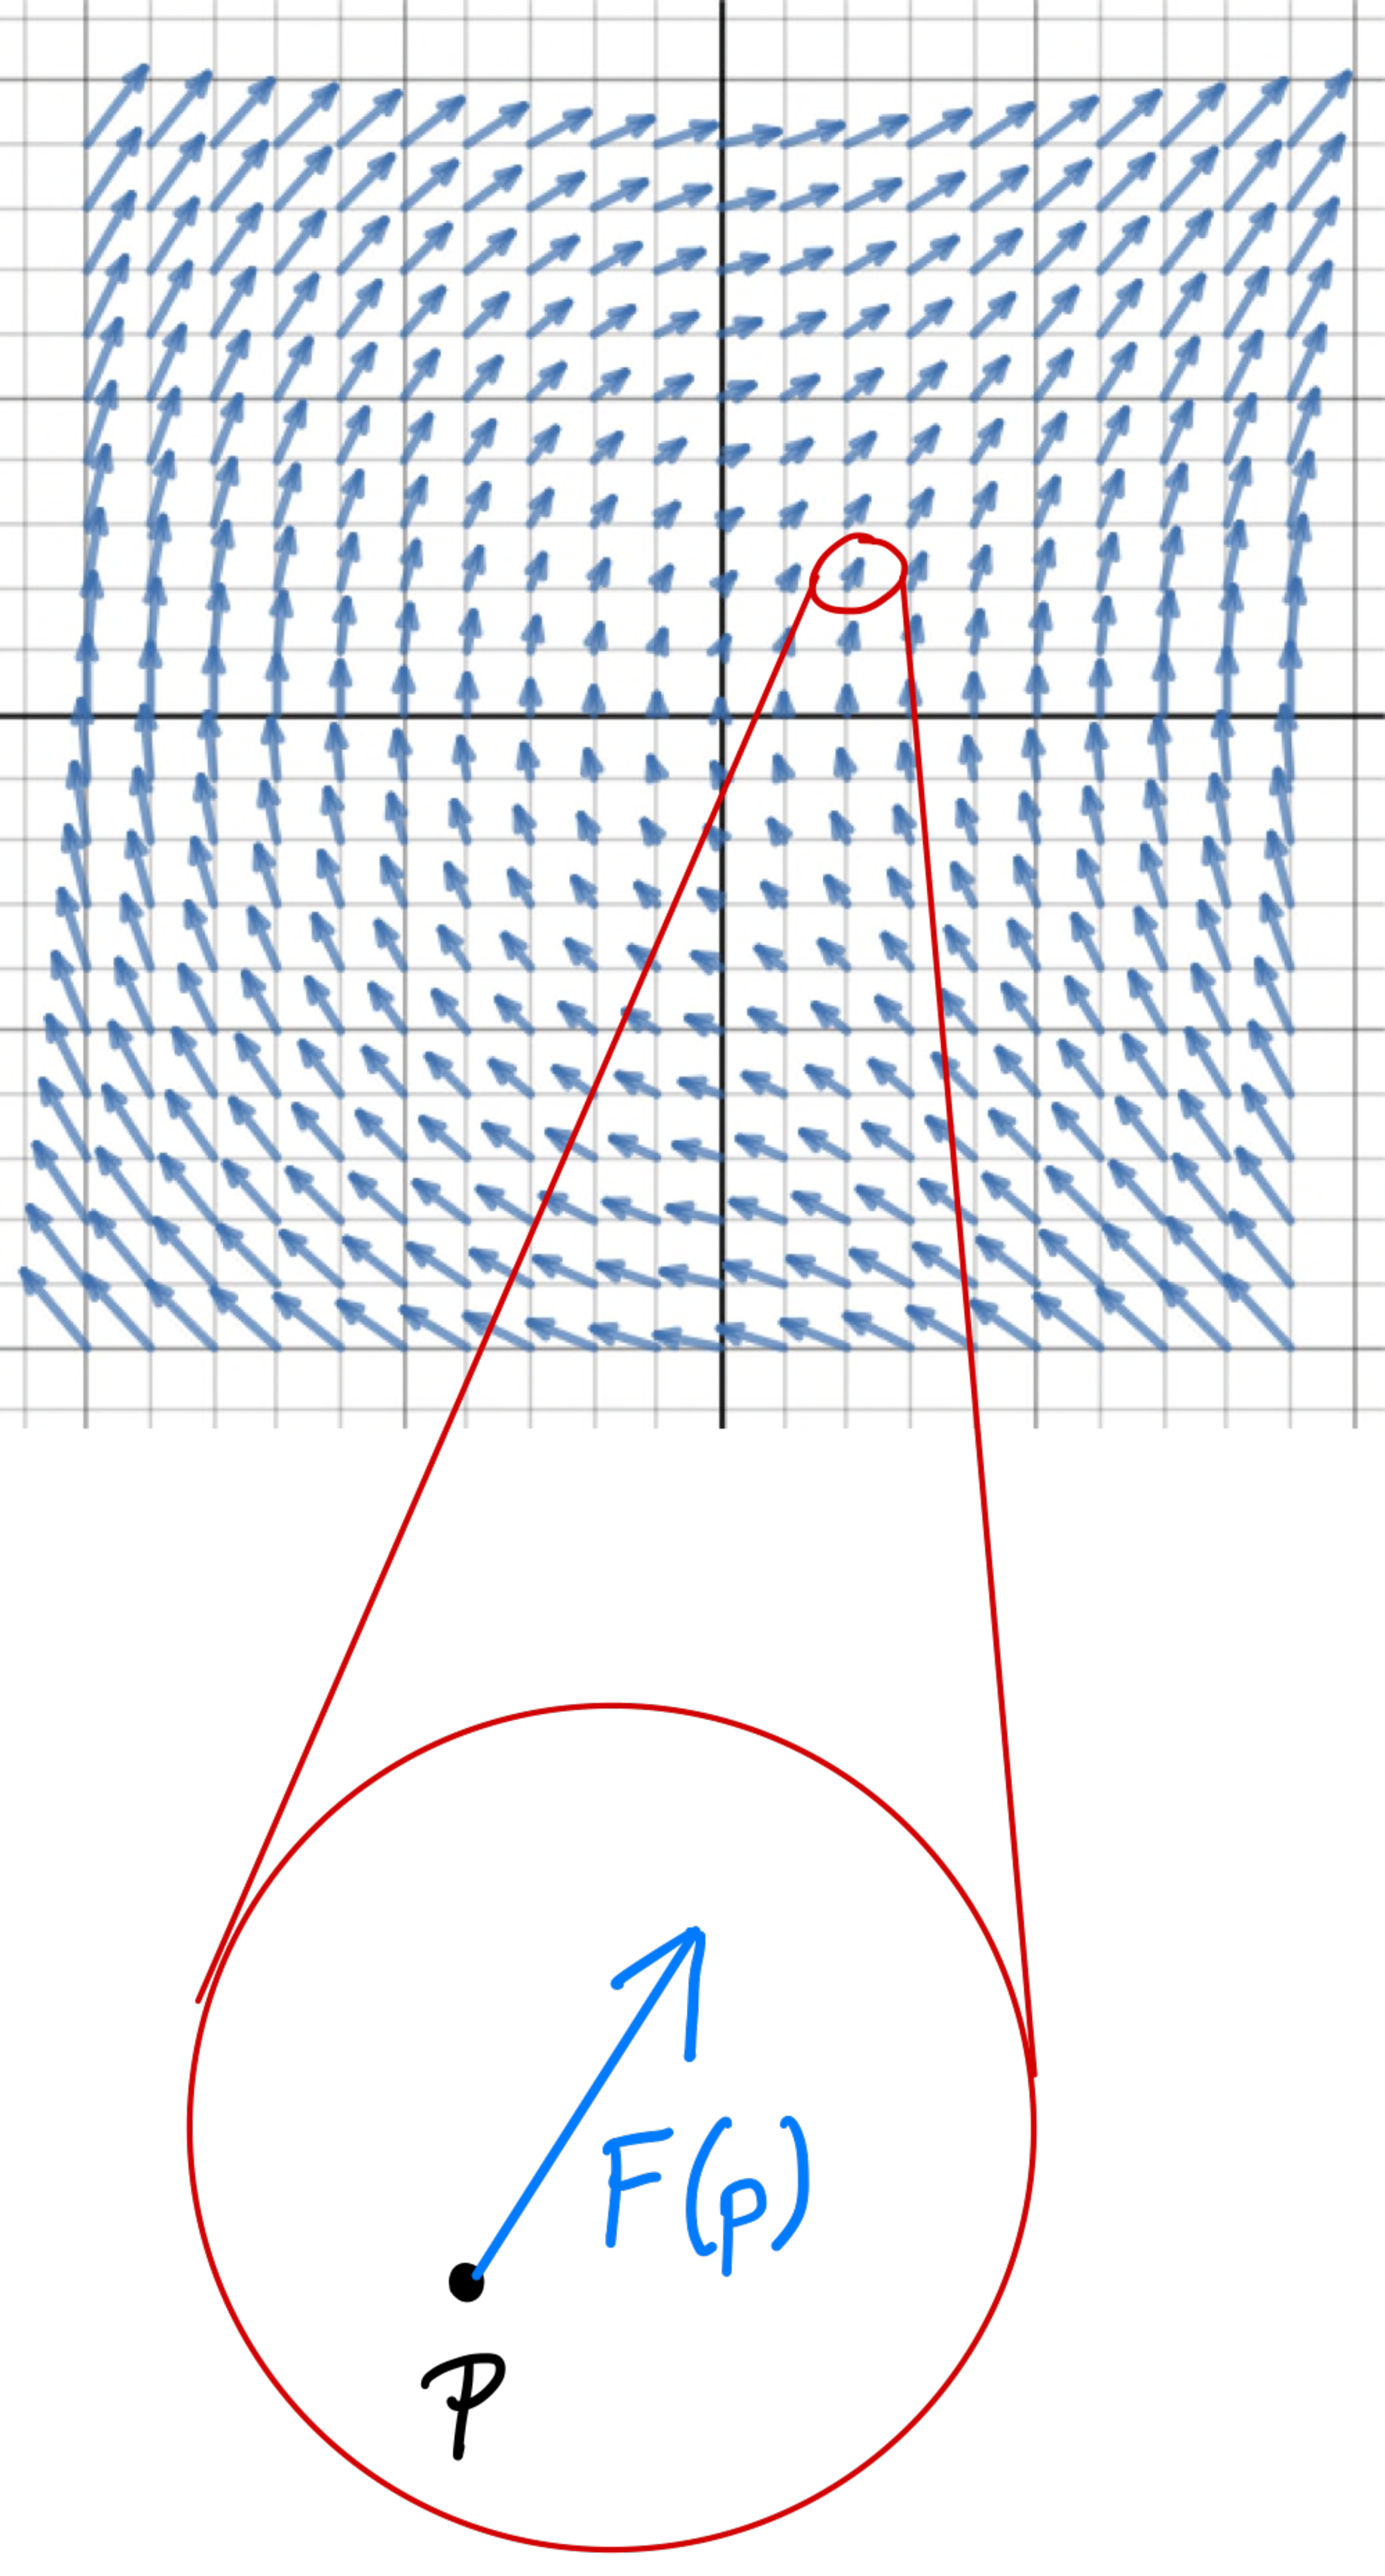
\includegraphics{2_9-vfield.pdf}
    \caption{A vector field ``attaches'' vectors to points.}
  \end{marginfigure}
  \noindent Notice, in particular, that functions $f\in C^\infty(M)$ are sections of the trivial bundle $M\times\R$.
\end{example}

One can sometimes distinguish non--isomorphic bundles by looking at the complement of their zero section: since any vector bundle isomorphism $h:E_1\to E_2$ must map the zero section of $E_1$ onto the zero section of $E_2$, the complements of the zero sections in $E_1$ and $E_2$ must be homeomorphic.

If the bundles are differentiable manifolds, then the definition of isomorphism nicely generalizes: they are \emph{diffeomorphic} if fibres are mapped to fibres diffeomorphically.

Even though, as we have seen, \emph{locally} $TM$ is diffeomorphic to $M\times\R^n$, this is not true in general with one exception.
\begin{exercise}\label{ex:trivialisable}
  Let $M$ be a smooth $n$-manifold that can be covered by a single smooth chart.
  Show that $TM$ is diffeomorphic to $M\times\R^n$ (without applying Proposition~\ref{prop:trivialisable}).
\end{exercise}

\begin{definition}
  A \emph{local frame} of a bundle $\pi:E\to M$ of rank $r$ is a family of $r$ local sections $(S_1, \ldots, S_r)\in\Gamma(E|_U)$ such that $(S_1(p), \ldots, S_r(p))$ is a basis for $E_p$ for all $p\in U$.
  If $U=M$ then $(S_1, \ldots, S_r)$ is called \emph{global frame}.
  Sometimes, the sections $S_j$ are called \emph{basis sections}.
\end{definition}

\begin{example}
  A chart on a $n$-manifold $M$ with local coordinates $(x^i)$ yields a local frame $\left\{\frac{\partial}{\partial x^1}, \ldots, \frac{\partial}{\partial x^n}\right\}$ of the tangent bundle $TM$.
\end{example}

In the spirit of what we have seen about the previous example, we have the following proposition.

\begin{proposition}
  Let $\pi:E \to M$ be a smooth vector bundle and $X:M\to E$ a section.
  If $(S_i)$ is a smooth local frame for $E$ over an open subset $U\subseteq M$, then $X$ is smooth on $U$ if an only if its component functions with respect to $(S_i)$ are smooth.
\end{proposition}
\begin{proof}
   Let $\varphi:\pi^{-1}(U) \to U\times\R^k$ be the local trivialization associated with the local frame $(S_i)$. Since $\varphi$ is a diffeomorphism, $X$ is smooth on $U$ if and only if $\varphi\circ X$ is smooth on $U$. If $(X^i)$ denote the component functions of $X$ with respect to $S_i$, then $\varphi\circ X (p) = (p, (X^1(p), \ldots, X^k(p)))$, so $\varphi\circ X$ is smooth if and only if the component functions $(X^i)$ are smooth.
\end{proof}

That is, given a local frame $\{S_1, \ldots, S_r\}\subset\Gamma(E|_U)$ of a vector bundle $\pi: E \to M$ we can express any section $X\in\Gamma(E)$ as a linear combination of elements of the frame:
\begin{equation}
  X = X^i S_i \quad\mbox{on }U,
\end{equation}
where $X^i\in C^\infty(U)$, $i=1,\ldots,r$.
Which was to be expected: after all, for each $p\in U\subset M$, the local frame is a basis for $E_p$.

\begin{proposition}\label{prop:trivialisable}
  A vector bundle $\pi: E\to M$ is trivialisable if and only if it admits a global frame.
\end{proposition}
\begin{proof}
  Let $\varphi: E \to M\times\R^r$ be a global trivialisation and $(e_1, \ldots, e_r)$ the canonical basis for $\R^r$.
  For $q\in M\times\R^r$, $(S_1(q), \ldots, S_r(q)) := \left(\varphi^{-1}\big|_q(e_1), \ldots, \varphi^{-1}\big|_q(e_r) \right)$ is a global frame for $E$ (why?).

  Conversely, let $(S_1, \ldots, S_r)$ be a global frame for $E$. Then
  \begin{equation}
    \varphi: E \to M\times\R^r, \quad
    \left(p, v^i S_i(p)\right) \mapsto \left(p, (v^1, \ldots, v^r)\right),
  \end{equation}
  is a global trivialisation for $E$.
\end{proof}

\begin{example}
  The cylinder $E = \bS^1\times\R$ is a trivialisable vector bundle with $\pi:E\to \bS^1$.
  Incidentally, the cylinder is isomorphic to $TS^1$ (why?).
\end{example}

A useful generalization of vector bundles, which we will not discuss in the course, is the locally trivial fiber bundle, where $\R$ is replaced by a more general manifold.

\section{Submanifolds}

With differentials of smooth functions at hand, we are ready to discuss submanifolds: smaller manifolds sitting inside larger ones.

\begin{definition}
  Let $M^m$ and $N^n$ be differentiable manifolds and $F:M\to N$ a $C^1$ function.
  \begin{itemize}
    \item $F$ is an \emph{immersion} if $dF_p$ is injective for all $p\in M$ ($\Rightarrow\; m\leq n$);
    \item $F$ is a \emph{submersion} if $dF_p$ is surjective for all $p\in M$ ($\Rightarrow\; m\geq n$);
    \item $F$ is an \emph{embedding} if $F$ is an injective immersion that is also a homeomorphism onto its range $F(M)\subset N$.
  \end{itemize}
\end{definition}
\begin{marginfigure}
  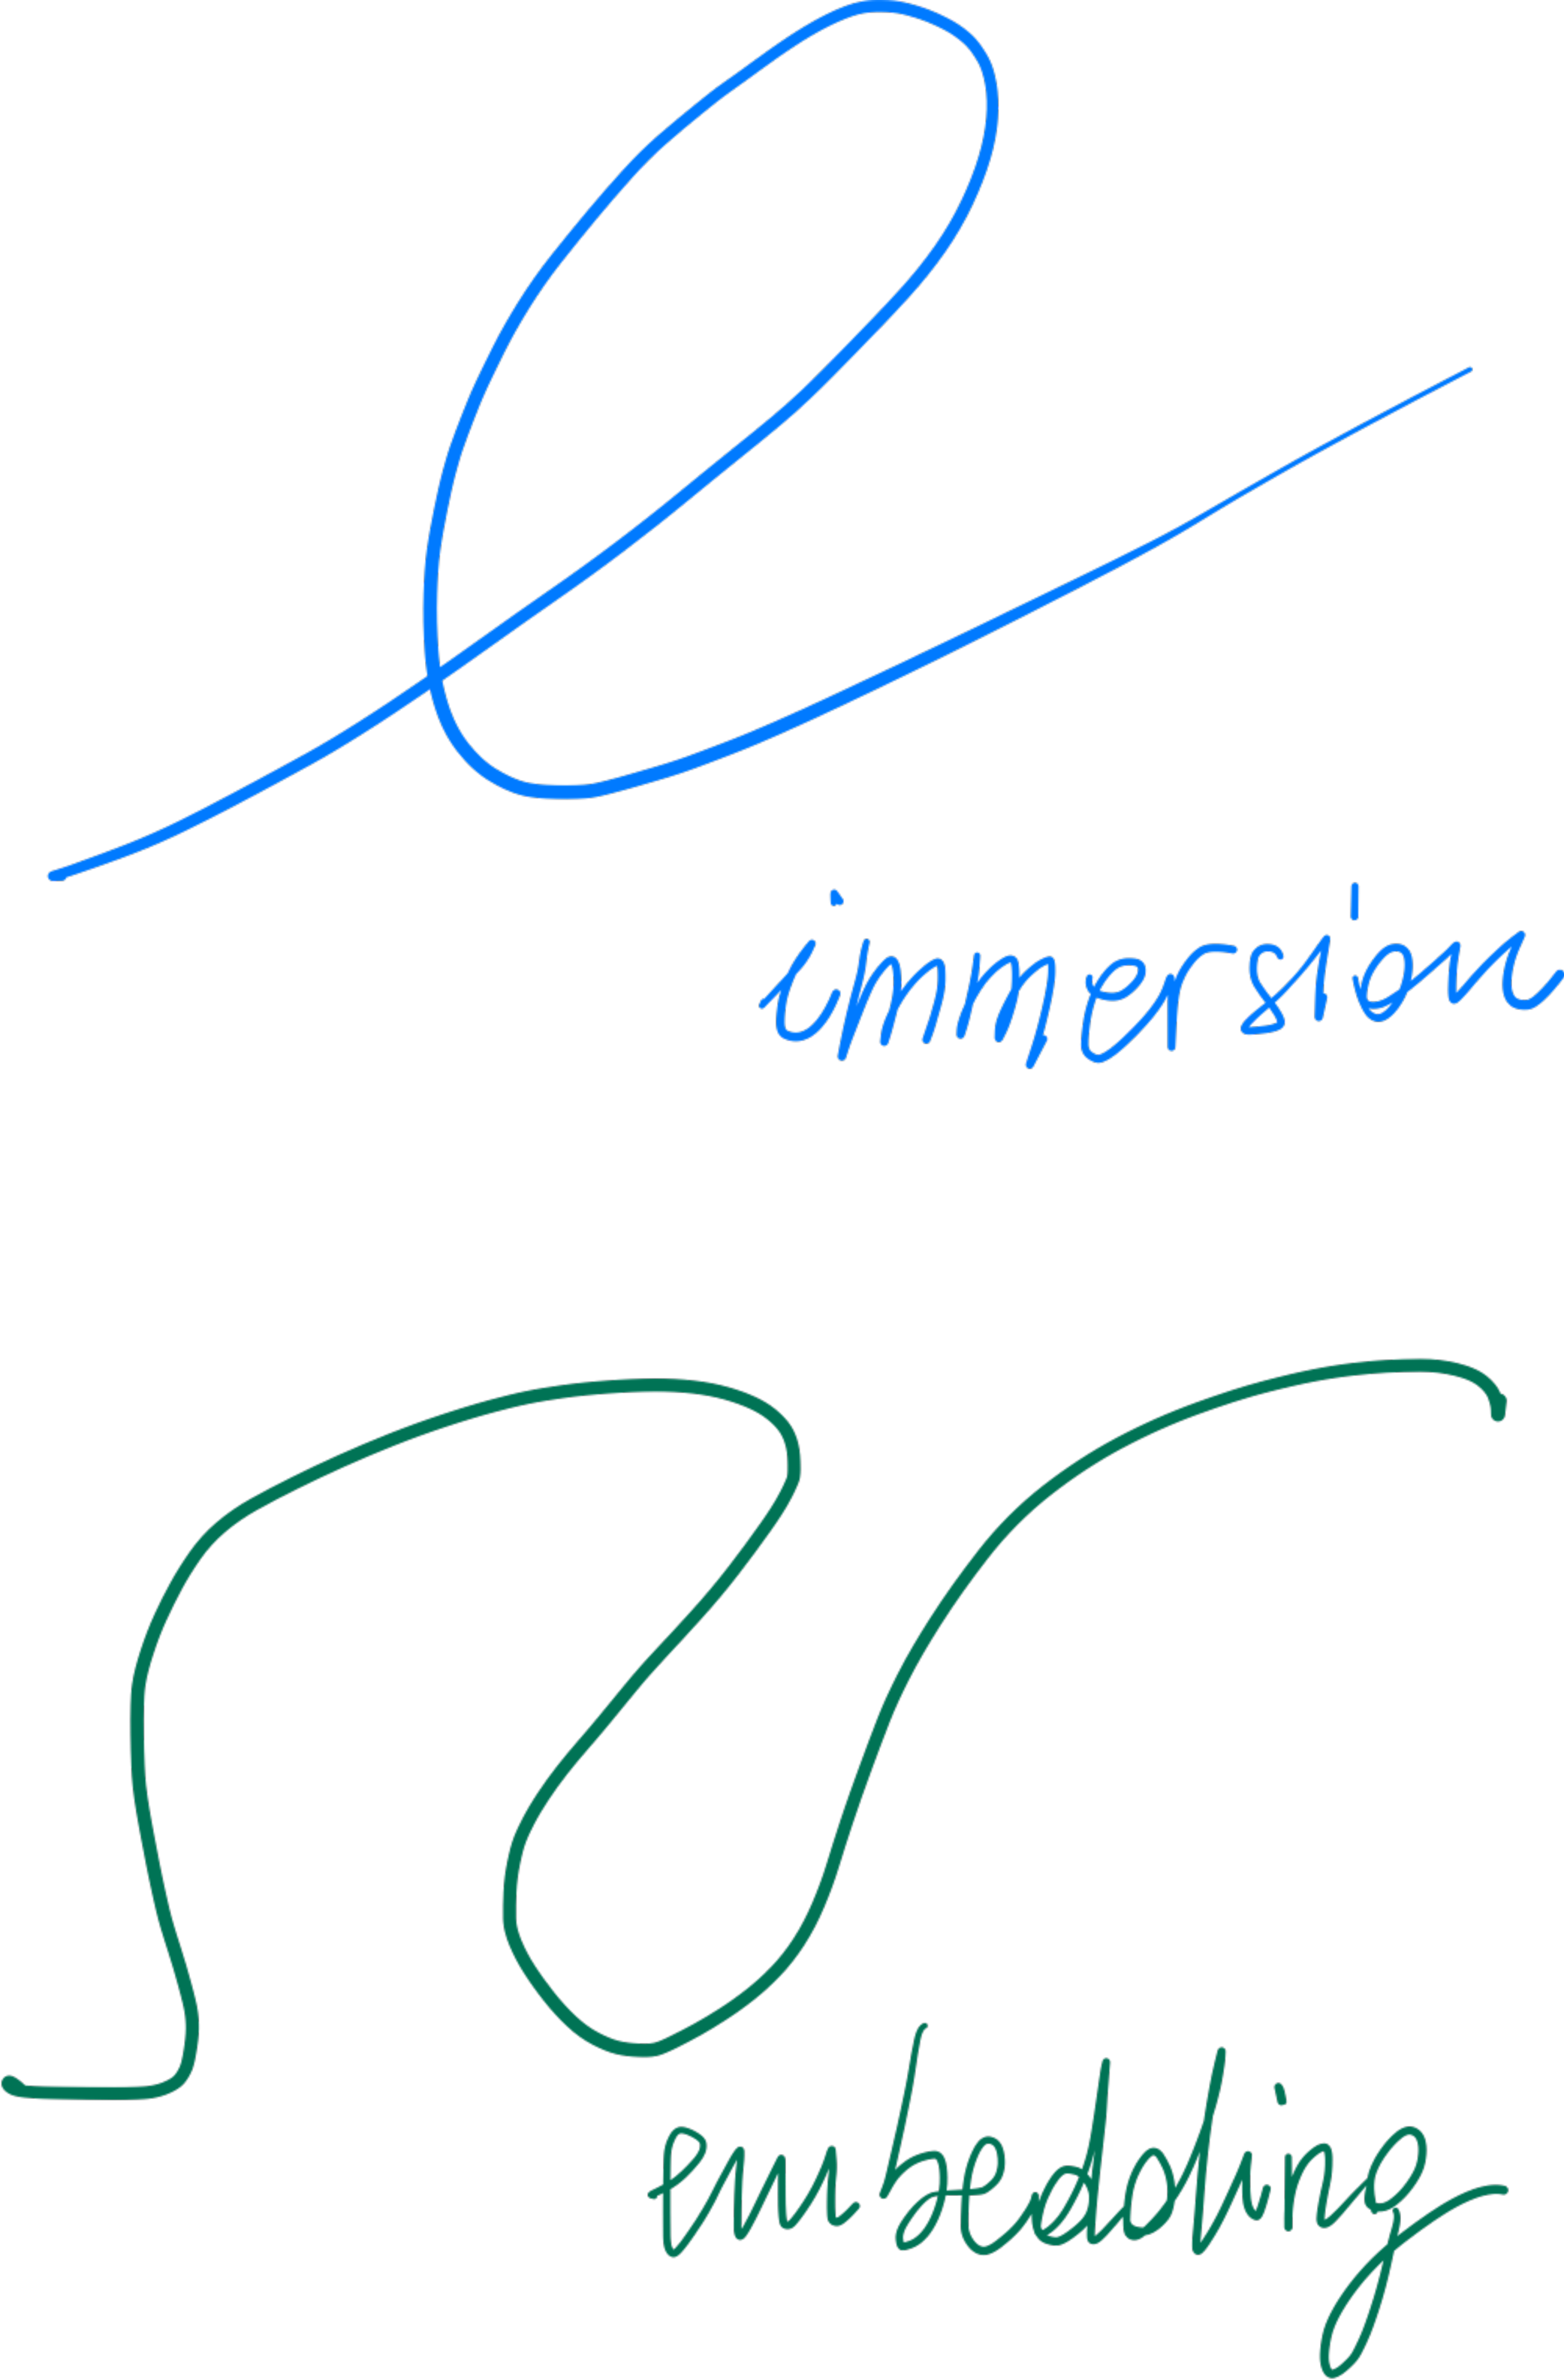
\includegraphics{2_8_1-immersion-embedding}
\end{marginfigure}

\begin{example}
  \begin{enumerate}
    \item The prototype of an immersion is the inclusion of $\R^m$ in a higher-dimensional $\R^n$:
    \begin{align}
      i &: \R^m \hookrightarrow \R^n,\\
      i &: \left(x^1, \ldots, x^m\right) \mapsto \left(x^1, \ldots, x^m, \LaTeXunderbrace{0, \ldots, 0}_{n-m}\right).
    \end{align}
    
    Indeed, the $n\times m$ matrix
    \begin{equation}
      di_x = Di(x)
       = \begin{pmatrix}
        1 & 0 & \cdots & 0 \\
        0 & 1 & \cdots & 0 \\
        \vdots & & \ddots & \vdots \\
        0 & \cdots & \cdots & 1 \\
        0 & \cdots & \cdots & 0 \\
        \vdots & & & \vdots \\
        0 & \cdots & \cdots & 0
       \end{pmatrix}
    \end{equation}
    has full rank (equal to $m$) and is therefore injective.
    Moreover, the map $i$ is injective and continuously invertible on its range, so it is also an embedding.

    \item The prototype for a submersion is the projection of $\R^m$ onto a lower-dimensional $\R^n$: $\pi\left(x^1,\ldots,x^n,x^{n+1},\ldots,x^m\right) = \left(x^1,\ldots,x^n\right)$.
    
    Indeed, the $n\times m$ matrix
    \begin{equation}
      d\pi_x = D\pi(x)
       = \begin{pmatrix}
        1 & 0 & \cdots & 0 & 0 & \cdots & 0 \\
        0 & 1 & \cdots & 0 & \vdots & & \vdots \\
        \vdots & & \ddots & \vdots & \vdots & & \vdots \\
        0 & \cdots & \cdots & 1 & 0 & \cdots & 0
       \end{pmatrix}
    \end{equation}
    has full rank (equal to $n$) and is therefore surjective.
    Hence, $i$ is a submersion.

    \item Let $n=1$, $m > 1$ and $\gamma:\R\to\R^m$ a smooth curve.
    The map $\gamma$ is an immersion if and only if its velocity vector satisfies $\gamma'(t)\neq0$ for all $t\in\R$.
    If the curve intersects itself, e.g $f(t_1) = f(t_2)$ for some $t_1\neq t_2$, then $f$ is not an embedding.
  \end{enumerate}
\end{example}

\begin{remark}
  Surjectivity of submersions or injectivity of immersions are properties of the differentials, not of the maps themselves.
  %
  For example, if $U\subset M$ open, the inclusion $i: U \to M$ is both an immersion and a submersion.
\end{remark}

\begin{definition}
  Let $M$ an $N$ smooth manifolds such that $M\subset N$ as a set.
  We say that $M$ is an \emph{embedded submanifold} of $N$ if the inclusion $M\hookrightarrow N$ is an embedding. If the inclusion is just an immersion, we say that $M$ is an \emph{immersed submanifold}.
\end{definition}

Before moving on, it is useful to recall some results from multivariable analysis.
A function $f:\R^m \to \R^n$ between euclidean spaces has rank $k$ at $x\in\R^m$ if its ($n\times m$) Jacobian matrix $Df(x)$ has rank $k$.
The function has \emph{maximal rank} at $x$ if $k = \min(n,m)$.
When $n=m$, $f$ has maximal rank at $x$ if and only if the square matrix $DF(x)$ is an invertible matrix.

As for many local properties, this definition carries over to manifolds rather ``smoothly''.

\begin{definition}
  A smooth map $F:M\to N$ has \emph{rank $k$} at a point $p$ if the linear subspace $dF_p(T_pM)$ has dimension $k$ inside $T_{F(p)}N$.
\end{definition}

And the same is true for the inverse function theorem:
compare the following statements.

\begin{theorem}[Inverse function theorem]\label{thm:ift}
  Let $U\subset\R^m$ open and $f:U \to \R^n$ be a smooth map.
  Assume that $f$ has maximal rank at some $x\in U$, then there exists a neighbourhood $\Omega\subset U$ of $x$ such that  $f\big|_\Omega : \Omega \to f(\Omega)$ is a diffeomorphism.
\end{theorem}

\begin{theorem}[Inverse function theorem for manifolds]\label{thm:iftm}
  Let $F:M\to N$ be a smooth function between manifolds of the same dimension $n$.
  Let $p\in M$ and assume that $F$ has maximal rank (i.e. rank $n$) at $p$.
  Then there exists a neighbourhood $V$ of $p$ such that the restriction $F:V\to F(V)$ is a diffeomorphism.
\end{theorem}
% \begin{proof}
%   This is a purely local statement.
%   Let $(U,\varphi)$ be a chart about $p\in M$ and let $(V, \psi)$ be a chart about $F(p)\in N$.
%   Since both $\varphi$ and $\psi$ are diffeomorphisms (and thus have maximal rank), the derivative of
%   \begin{equation}
%     \psi \circ F \circ \varphi^{-1}: \varphi(U\cap F^{-1}(V)) \to \psi(F(U)\cap V)
%   \end{equation}
%   has rank $n$ at $\varphi(p)$.
%   Thus the inverse function theorem, Theorem~\ref{thm:ift}, there exists $\Omega \subset \varphi(U\cap F^{-1}(V))$ such that $\psi \circ F \circ \varphi^{-1}\big|_{\Omega}$ is a diffeomorphism.
%   Therefore, once again since both $\varphi$ and $\psi$ are diffeomorphisms, $F\big|_W : W \to F(W)$ is also a diffeomorphism for $W := \varphi^{-1}(\Omega)$.
% \end{proof}
\begin{exercise}
  Use the euclidean inverse function theorem\footnote{Theorem~\ref{thm:ift}.} on $\R^n$ to prove Theorem~\ref{thm:iftm}.
\end{exercise}


In fact, also analogues of the implicit functions theorem carry over.
We will state them without going into the details of the proofs.

\begin{marginfigure}
  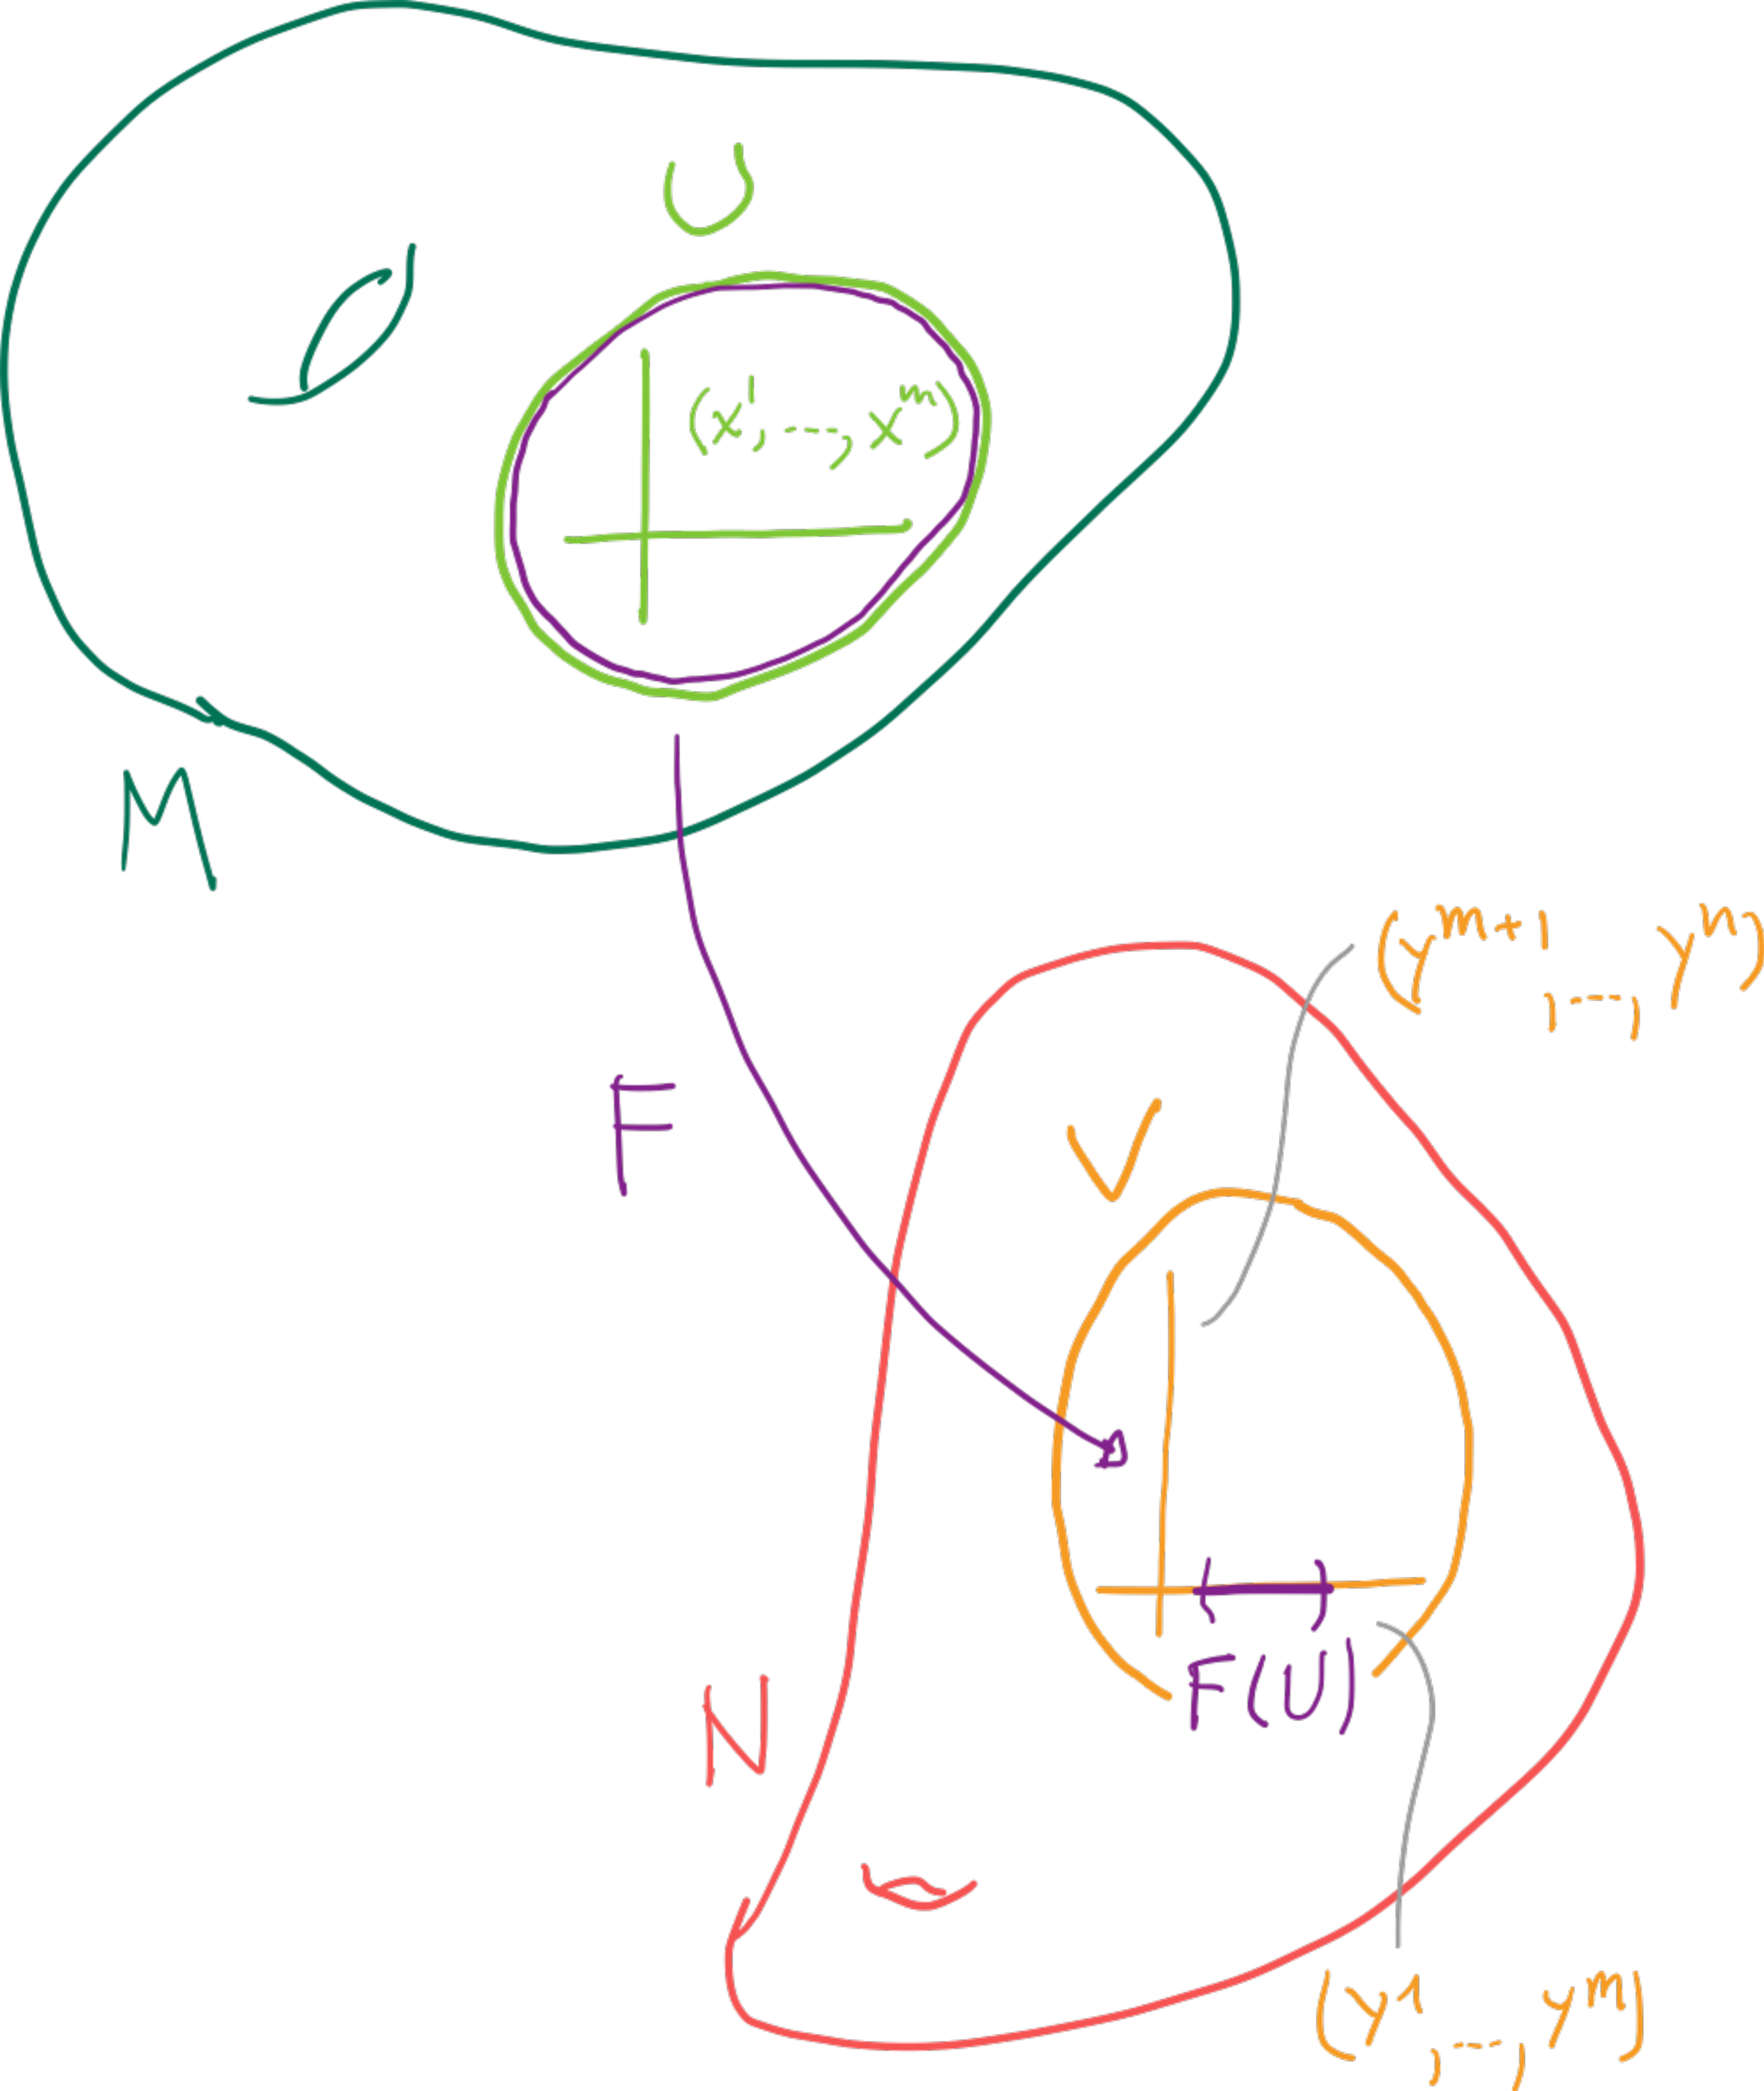
\includegraphics{2_8_9-mapping.pdf}
\end{marginfigure}
\begin{proposition}\label{prop:slice_chart}
  Let $F:M^m\to N^n$ be an immersion.
  Then for any $p\in M$, there exists a neighbourhood $U$ of $p$ and a chart $(V,\psi)$ about $F(p)\in N$ such that
  \begin{enumerate}[(i)]
    \item If $y^i = r^i\circ \psi$ are the local coordinates of $\psi$ then
    \begin{equation}\label{eq:slice_chart}
      F(U)\cap V = \left\{ q \in V \;\mid\; y^{m+1}(q)=\cdots=y^n(q)=0\right\};
    \end{equation}
    \item $F\big|_U$ is an embedding.
  \end{enumerate}
 \end{proposition}

If $F$ is an embedding, and this $M$ is an embedded submanifold, then the set $F(U)$ above can be written as $F(U) = F(M)\cap W$ for some open set $W\subset N$.
By replacing $V$ in~\eqref{eq:slice_chart} with $V\cap W$, one gets 
\begin{equation}
  F(M)\cap V = \left\{ q \in V \;\mid\; y^{m+1}(q)=\cdots=y^n(q)=0\right\}.
\end{equation}
In particular, this means that a $m$-dimensional submanifold is also a $m$-dimensional manifold whose charts are the ones above after we drop the final $n-m$ components.

The proposition above shows that an immersion is always a local embedding.
\begin{exercise}
  \begin{enumerate}
    \item If $M$ is compact, an injective immersion $F:M\to N$ is always an embedding.
    \item This is not necessarily the case in the non-compact case, give a counterexample.
  \end{enumerate}
\end{exercise}

\begin{lemma}
  With the notation of Proposition~\ref{prop:slice_chart}, assume that around any point $p\in M$ there is a chart of the form
  \begin{equation}
    M\cap V = \left\{ q \in V \;\mid\; y^{m+1}(q)=\cdots=y^n(q)=0\right\} \subset N.
  \end{equation}
  Then, if we endow $M$ with the subspace topology on $N$, $M$ is a topological manifold of dimension $m$.
  Furthermore, it has a smooth structure that makes it into an embedded submanifold of $N$.
\end{lemma}
\begin{proof}[Sketch]
  Let $\pi: \R^n\to\R^m$ be the projection as in the examples above.
  Let $p\in M$ and let $(V,\psi)$ be a chart with coordinates $(y^i)$ of the form above.
  If we endow $M$ with the subspace topology, then $\sigma:= \pi \circ \psi\big|_{M\cap V}$ is a homeomorphism.
  Repeating this at any point we end up with a collection of maps satisfying the hypotheses of Lemma~\ref{lem:manifold_chart}.
  Thus $M$ is a smooth manifold of dimension $n$ and its topology coincides with the subspace topology.

  Finally, with the inclusion $i:M\hookrightarrow N$ one has that $\psi \circ i\circ \sigma^{-1} (p^1,\ldots,p^n) = (p^1,\ldots,p^n,0,\ldots,0)$ which is smooth.
\end{proof}

A non-trivial consequence of the previous lemma is the following proposition\footnote{Refer to \cite[Proposition 5.8 and Proposition 5.31]{book:lee}.}.

\marginnote[1em]{In Proposition~\ref{prop:uniqdiffeoinclusion} it is not enough to ask that $\iota$ is smooth! As counterexample consider the two manifolds $(\R, \cA_1)$ with $\cA_1 := \{(\R, \id_\R)\}$ and $(\R, \cA_2)$ with $\cA_2 := \{(\R, x\mapsto x^3)\}$. The inclusion of open sets in $\R$ is smooth in both cases but is a diffeomorphism only in one.}
\begin{proposition}\label{prop:uniqdiffeoinclusion}
  Let $M$ be a manifold and $U\subset M$ an open set.
  Then $U$ has a unique differentiable structure such that the inclusion $\iota:U\hookrightarrow M$ is a diffeomorphism.
\end{proposition}

Up to this point, the first manifold had the same dimension or was smaller than the second one.
What if it is larger?

\begin{definition}
  Let $F:M^m \to N^n$ be a smooth map between smooth manifolds.
  A point $p\in M$ is said to be a \emph{regular point} of $F$ if $F$ has rank $n$ at $p$ (which implies that $m\geq n$), while it is called a \emph{critical point} if it is not.

  Similarly, a point $q\in N$ is called a \emph{regular value} if every point in $F^{-1}(q)$ is a regular point, and \emph{critical value} otherwise. If $q\not\in F(M)$, then $q$ is considered a regular value (in the sense that there is nothing to check in its preimage by $F$).
  Cf. Figure~\ref{fig:2_8-crit_pts}.
\end{definition}
\begin{marginfigure}[12em]
  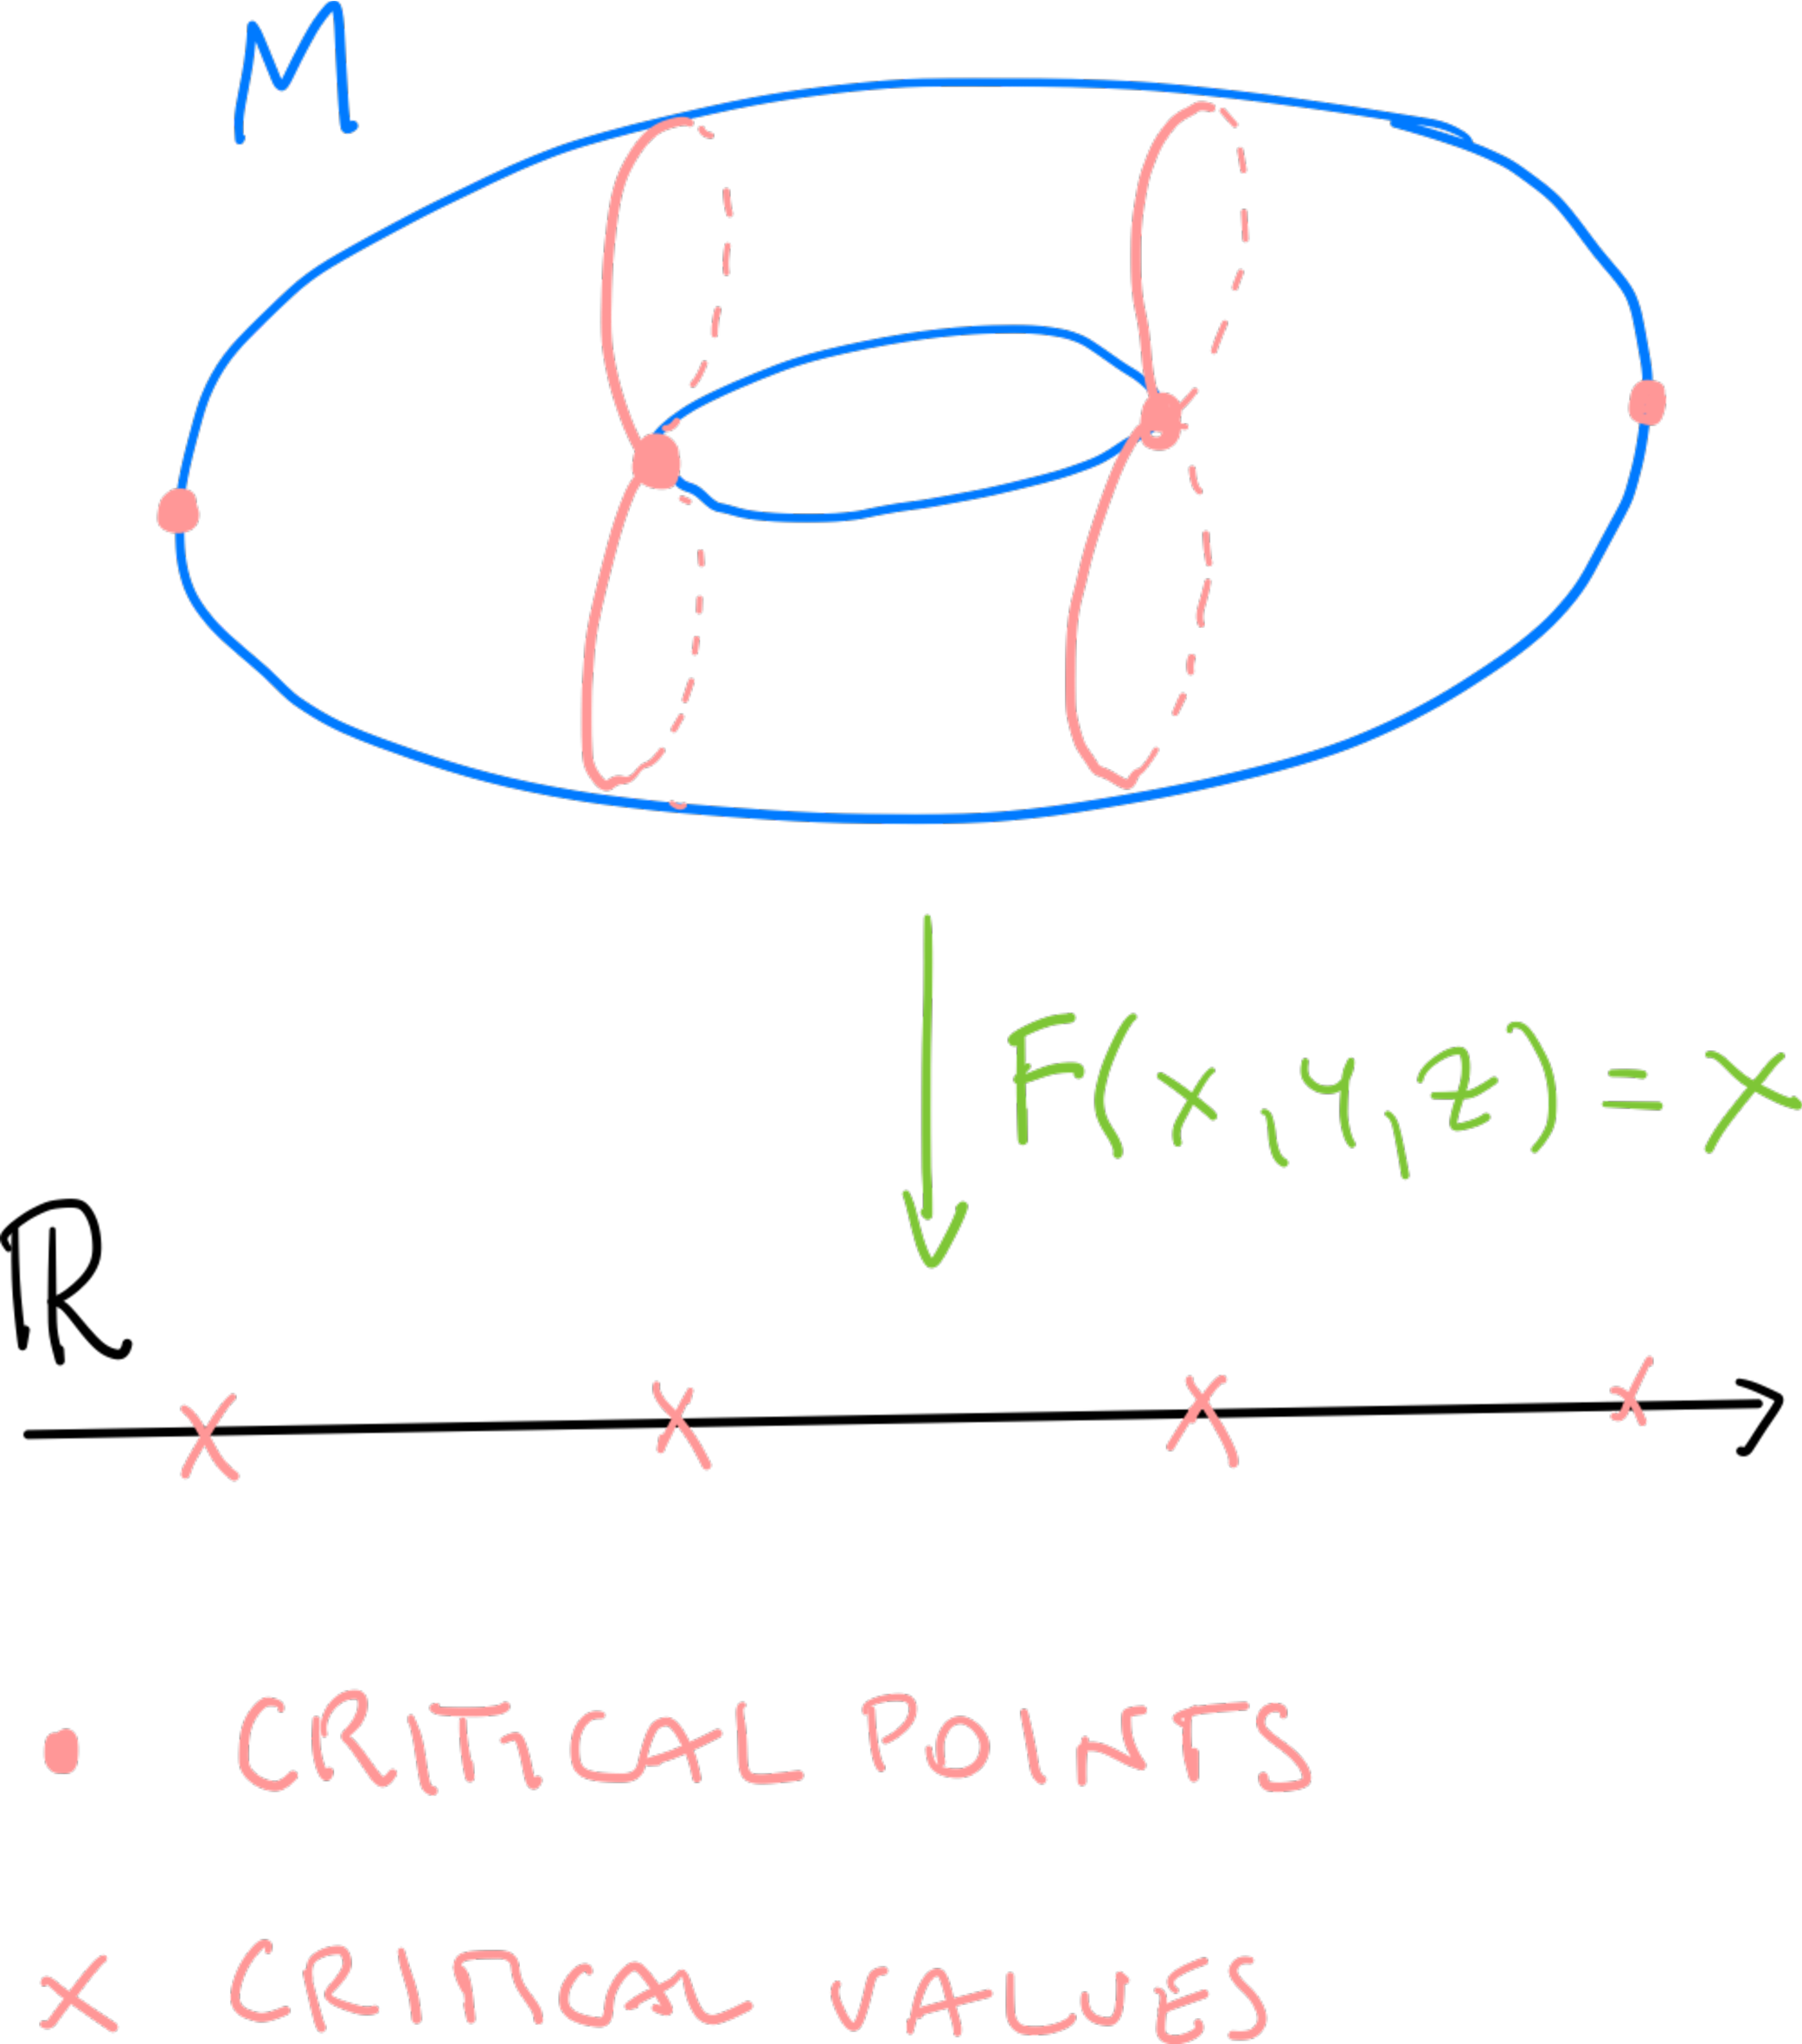
\includegraphics{2_8-crit_pts.pdf}
  \caption{Beware of the subtleties here. The map $F=\pi_x\circ i$ for the inclusion $i:\bT^2\hookrightarrow\R^3$ and the projection $\pi_x(x,y,z)=x$.
  So $dF_p = d (\pi_x)_{i(p)} \circ d i_p$. The latter is zero if $d i_p: T_p\bT^2\hookrightarrow T_p\R^3$ is, which happens when the image of $T_p\bT^2$ is contained in the $yz$-plane (the reason will be clear by the end of the chapter): the critical points depicted here are exactly those points for which the tangent plane is the $yz$-plane.}
  \label{fig:2_8-crit_pts}
\end{marginfigure}

With this definition at hand, we are ready to state one of the most important theorems in this lecture. Differently from most previous ones, the statement is not local.

\begin{theorem}[Implicit function theorem for manifolds]\label{thm:impl_fun}
  Let $m\geq n$ and let $F: M^m \to N^n$ be a smooth map between smooth manifolds.
  If $q\in N$ is a regular value of $F$ and $P := F^{-1}(q)$ is not empty, then $P$ is a topological manifold of dimension $n-k$. 
  Moreover, there exists a smooth structure on $P$ which makes it into a smooth embedded submanifold of $M$.
\end{theorem}

\begin{remark}
  If $F:M\to N$ is a submersion, Theorem~\ref{thm:impl_fun} implies that any $p\in M$ belongs to the $(n-k)$-dimensional embedded submanifold $F^{-1}(F(p))$.
\end{remark}

From this observation follows another interesting proposition, again consequence of the inverse and the implicit function theorems, of which we will also omit the proof.

\begin{proposition}\label{prop:submanifolds_and_R}
  The following assertions are equivalent.
  \begin{enumerate}[(i)]
    \item $M^k\subset N^n$ is a $k$-dimensional submanifold.
    \item $M$ is locally the image of an embedding of a subset of $\R^k$.
    That is, for every $p\in M$ there exists $V\subset M$ open neighbourhood of $p$, an open set $U\subset\R^k$ and an embedding
    \begin{equation}
      \varphi : U \to N \quad\mbox{such that}\quad \varphi(U)=V.
    \end{equation}
    \item $M$ is locally a level set of a submersion into $\R^{n-k}$.
    That is, for every $p\in M$ there exists $V\subset M$ open neighbourhood of $p$ and a submersion $\varphi: V \to\R^{n-k}$ such that
    \begin{equation}
      M\cap V = \{q\in V \;\mid\; \varphi(q) = 0\}.
    \end{equation}
  \end{enumerate}
\end{proposition}

\begin{remark}\label{rmk:WhitneyET}
  Whitney Embedding Theorem states that any smooth $n$-dimensional manifold can be smoothly embedded into $\R^{2n}$.
  Thus any abstract manifold is diffeomorphic to a submanifold of $\R^m$ (for some $m$).
\end{remark}

\begin{example}\label{ex:s2}
  The sphere $\bS^2 = \{x\in\R^3 \mid \|x\| = 1\}$ is a $2$-dimensional submanifold of $\R^3$.
  This is immediate using the third condition in the Proposition~\ref{prop:submanifolds_and_R}: let $\varphi(x) = \|x\|^2 -1 : \R^3 \to \R$, then $\varphi$ is smooth, $\bS^2 = \{F(x)=0\}$ and $dF_x(v)= 2x\cdot v \neq 0$ for $x\in\bS^2$.
\end{example}

\begin{example}
  Let $N = \R^2$ and $M = \{ x\in M \;\mid\; x^2 = |x^1| \}$.
  Then $M$ is \emph{not} a submanifold, but it can be equipped with a manifold structure.
  For example with the global atlas $\{(M,\; (x^1,x^2)\mapsto x^1)\}$, $M$ is a manifold diffeomorphic to $\R$.
\end{example}

\begin{exercise}
  A real-valued function $f:M\to\R$ on a manifold has a local maximum at $p\in M$ if there is a neighbourhood $U\subset M$ of $p$ such that $f(p) \geq f(q)$ for all $q\in U$.
  \begin{enumerate}
    \item Show that if a differentiable function $f:(a,b)\to\R$, has a local maximum at $x\in (a,b)$, then $f'(x) = 0$.
    \item Prove that a local maximum of a function $f\in C^\infty(M)$ is a critical point of $f$.\\
    \textit{\small Hint: choose $X_p\in T_pM$ and let $\gamma(t)$ be a curve in $M$ starting at $p$ with initial velocity $X_p$. The $f\circ \gamma$ is a real-valued function with local maximum at $0$...}
  \end{enumerate}
\end{exercise}

Of course, we can also define subbundles.
\begin{definition}
  Let $\pi:E \to M$ be a rank-$n$ vector bundle and $F\subset E$ a submanifold.
  If for all $p\in M$, the intersection $F_p := F\cap E_p$ is a $k$-dimensional subspace of the vector space $E_p$ and $\pi|_F : F \to M$ defines a rank-$k$ vector bundle, then $\pi|F: F \to M$ is called a \emph{subbundle} of $E$.
\end{definition}

\begin{exercise}[\textit{[homework 2]}]
  Let $M$ be a smooth $m$-manifold and $N$ a smooth $n$-manifold.
  Let $F:M\to N$ be an embedding and denote $\widetilde M = F(M)\subset N$.
  \begin{enumerate}[(a)]
    \item Show that the tangent bundle of $M$ in $N$, given by $T\widetilde M := dF(TM) \subset TN\Big|_{\widetilde M}$, is a subbundle of $TN\Big|_{\widetilde M}$ by providing explicit local trivialisations in terms of the charts $(U, \varphi)$ for $M$.
    \item Assume that there exist a smooth function $\Phi:N\to\R^{n-k}$ such that $\widetilde M := \{p\in N \mid \Phi(p) = 0\}$ and $d\Phi_p$ has full rank for all $p\in\widetilde M$. Prove that
    \begin{equation}
      T\widetilde{M} = \{(p,v)\in TN|_{\widetilde{M}} \mid v\in\ker(d\Phi_p)\}.
    \end{equation}
  \end{enumerate}
\end{exercise}

We still have a question pending since the beginning of the chapter.
Is the tangent space to a sphere the one that we naively imagine (see Figure~\ref{fig:tan-embedded-sphere})?
To finally answer the question, we will prove one last proposition.

\begin{proposition}
  Let $F:M^m\to N^n$ be a smooth map between manifolds.
  Let $q\in N$ be a regular value of $F$ such that $P:=F^{-1}(q)\neq\emptyset$ and let $i:P\hookrightarrow M$ denote the inclusion.
  Then, for all $p\in P$, one has
  \begin{equation}
    d i_p(T_p P) = \ker dF_p.
  \end{equation}
\end{proposition}
\begin{proof}
  Both $d i_p(T_p P)\subset T_p M$ and $\ker dF_p \subset T_p M$ are linear subspaces of the same dimension $n-k$, therefore we only need to show that one contains the other, e.g. $d i_p(T_p P) \subset \ker dF_p$.

  Take $f\in C^\infty(N)$ and $v\in T_p P$. By the chain rule\footnote{Proposition~\ref{thm:chainrule_mfld}} we get
  \begin{equation}
    (d F_p \circ d i_p)(v)(f) = d(F\circ i)_p(v)(f) = v(f\circ F\circ i).
  \end{equation}
  Since $F\circ i\big|_{P} \equiv q$ constant, $f\circ F\circ i\in C^\infty(P)$ is the constant function $p \mapsto f(q)$ and by Corollary~\ref{cor:derzero} we have $v(f\circ F\circ i)=0$.
\end{proof}

\begin{example}
  We have seen in Example~\ref{ex:s2} that $\bS^2 = F^{-1}(0)$ is a smooth manifold of dimension $2$.
  Denoting the inclusion by $i:\bS^2 \hookrightarrow\R^3$, one has
  \begin{equation}\label{ex:tan_sph}
    di_x(T_x\bS^2) = \cT_p(p^\perp)
  \end{equation}
  where $\cT_p:\R^3\to T_p\R^3$ is the map defined in Exercise~\ref{ex:tg_curve_iso} and
  \begin{equation}
    p^\perp := \big\{q\in\R^3 \;\mid\; \left\langle p, q\right\rangle = 0\big\},
  \end{equation}
  where $\left\langle\cdot,\cdot\right\rangle$ is the usual Euclidean dot product.
  Take a long deep breath and unfold the definitions in~\eqref{ex:tan_sph}, here it may be useful to draw a picture\footnote{Which is generally always the case in geometry and topology, and most other mathematical fields.}. 
  Equation~\eqref{ex:tan_sph} implies that the tangent space to $\bS^2$ at a point $x$  is the plane tangent to $\bS^2$ at $p$, as claimed in Figure~\ref{fig:tan-embedded-sphere}.
\end{example}

\begin{exercise}
  Show that the above reasoning holds verbatim for $\bS^n\subset\R^{n+1}$.
\end{exercise}

\begin{exercise}
  Let $U\subset\R^n$ open and $f:U\to\R$ smooth.
  Define $g:U\to\R^{n+1}$ by
  \begin{equation}
    g(x) = (x, f(x)).
  \end{equation} 
  Show that $g$ is a smooth embedding and, therefore, that $g(U)$ is a smooth embedded $n$-dimensional submanifold\footnote{$g(U)$ is the the \emph{graph} of $f$!} of $\R^{n+1}$.
\end{exercise}

\begin{exercise}[\textit{[homework 2]}]\label{exe:onsubmanifold}
  Show that the orthogonal matrices $O(n) := \{ Q\in GL(n) \mid Q^TQ=\id \}$ form a $n(n-1)/2$-dimensional submanifold of the $n^2$-manifold $\mathrm{Mat}(n)$ of $n\times n$-matrices.

  Show also that
  \begin{equation}
    T_Q O(n) = \left\lbrace B \in \mathrm{Mat}(n) \mid (Q^{-1} B)^T = -Q^{-1}B \right\rbrace,
  \end{equation}
  and, thus, that $T_{\id} O(n)$ is the space of skew-symmetric matrices
  \begin{equation}
    T_{\id} O(n) = \left\{ B \in \mathrm{Mat}(n) \mid B^T = -B \right\}.
  \end{equation}
  \textit{\small Hint: Find a suitable map $F: \mathrm{Mat}(n) \to \mathrm{Sym}(n)$ such that $F^{-1}(\{p\}) = O(n)$ for some point $p$ in the image, e.g. $0$ or $\id_n$.
  Here $\mathrm{Sym}(n)$ denotes the space of symmetric matrices.}
\end{exercise}


\chapter{Vector fields}\label{ch:vf}
We continue with our quest of generalizing multivariable calculus.
The next familiar object waiting to be questioned are vector fields.
In the euclidean settings these are simply continuous maps that attach a vector to each point in their domain.

The step to abstract manifold is rather intuitive in this case: a vector field will be a map that, at each point of a manifold, picks a tangent vector at that point in a smooth way.

\begin{definition}
  A $C^p$-map $X: M \to TM$ with $\pi\circ X = \id_M$, or equivalently $X_p\in T_pM$ for all $p\in M$, is called \emph{$C^p$-vector field}.
  We denote\footnote{Alternative notations are $\cT_0^1(M)$, $\cT(M)$ and $\Gamma(TM)$. The first two are related to vector fields being tensor fields of type $(1,0)$, a topic that we will discuss in the near future.} the set of smooth vector fields by $\fX(M)$.
\end{definition}

\begin{remark}
  A careful look at the definition shows that vector fields are sections of $TM$, indeed $\fX(M) \equiv \Gamma(TM)$.
  This is a useful way to start understanding the bundle terminology: in some sense, sections of vector bundles are a generalisation of vector fields.
\end{remark}

Beware of the curse of differential geometry.
For convenience and to be consistent with our notation for elements of the tangent bundle, we denote the value $X_p\in\{p\}\times T_p M$ of a vector field by $X_p$ instead of $X(p)$.
Furthermore, we will often identify $X_p$ with its component in $T_pM$, thus considering it as if $X_p\in T_pM$, without explicitly projecting it to the second component.

Let $M$ be a smooth $n$-manifold (with or without boundary).
Let $X:M\to TM$ be a vector field, not necessarily smooth, and $(U, (x^i))$ a smooth coordinate chart for $M$. Then we can write the value of $X$ at any point $p\in U$ as a linear combination in terms of the coordinate basis vector:
\begin{equation}\label{eq:vfCoordBAsis}
  X_p = X^i(p) \frac{\partial}{\partial x^i}\Big|_p.
\end{equation}
This defines $n$ functions $X^i: U\to\R$, called \emph{component functions of $X$} in the chart.

\begin{exercise}
  Show that, in the notation above, the restriction of $X$ to $U$ is smooth if and only if its component functions with respect to the chart are smooth.
\end{exercise}

\begin{example}
  If $(U, (x^i))$ is a smooth coordinate chart for a manifold $M$, the assignment $p \mapsto \frac{\partial}{\partial x^i}\big|_p$ determines a vector field on $U$, called the \emph{$i$th-coordinate vector field} and commonly denoted $\partial_{i}$, $\partial_{x^i}$ or $\partial/\partial x^i$.
  Despite their looks, the $\partial_{x^i}|_p$ denote genuine vectors in $T_p M$ that can be associated to euclidean vectors via a suitable chart.
\end{example}

The space of smooth vector fields is a vector space under pointwise addition and scalar multiplication: for all $p\in M$, $X,Y\in\fX(M)$, $\alpha, \beta \in \R$, we have
\begin{equation}
  (\alpha X + \beta Y)_p = \alpha X_p + \beta Y_p.
\end{equation}
The zero element of the vector space, called \emph{zero vector field}, is the vector field whose values is $0\in T_pM$ for all $p\in M$.
Moreover, each vector field can be multiplied by smooth functions $f\in C^\infty(M)$ by defining $fX:M\to  TM$ by
\begin{equation}
  (fX)_p = f(p)X_p.
\end{equation}

\begin{proposition}
  Let $M$ be a smooth manifold with or without boundary.
  \begin{enumerate}
    \item If $X,Y \in \fX(M)$ and $f,g\in C^\infty(M)$, then $fX+gY \in\fX(M)$.
    \item $\fX(M)$ is a module over the ring $C^\infty(M)$.
  \end{enumerate}
\end{proposition}

In this sense, the basis expression \eqref{eq:vfCoordBAsis} can be also rewritten as an equation between fields instead of an equation between vectors at point:
\begin{equation}\label{eq:vfCoordBAsis}
  X = X^i \frac{\partial}{\partial x^i},
\end{equation}
where $X^i$ denotes the component of the vector field $X$ in the given coordinates.

There is one more way of thinking about the coordinate basis expression above.
We have seen that differentials of smooth maps define maps between tangent bundles.
As it turns out, we can employ differentials of diffeomorphisms to map vector fields to vector fields.

\begin{definition}
  Let $F:M\to N$ be a diffeomorphism of smooth manifolds.
  Then, the \emph{pushforward} $F_*$ of $F$, defined by\footnote{In coordinates, this reads\begin{equation}
      (F_* X)_q = dF_{F^{-1}(q)}(X_{F^{-1}(q)}).
    \end{equation}}
  \begin{equation}
    F_*: \fX(M) \to \fX(N),\qquad
    X \mapsto F_* X = d F \circ X \circ F^{-1},
  \end{equation}
  maps (``pushes forward'') vector fields on $M$ to vector fields on $N$.
\end{definition}

The definition of pushforward is more easily pictured by means of the following commutative diagram:
\begin{equation}
  \begin{tikzcd}[row sep=huge, column sep=huge]
    M \arrow[d, "X"]
    & N \arrow[l, "F^{-1}"] \arrow[d, "F_*X" red]\\
    TM \arrow[r, "d F"]
    & TN
  \end{tikzcd}.
\end{equation}

Then, if $(U, \phi)$ is a coordinate chart for $M$, the restriction of a vector field $X\in\fX(M)$ to $U$ can be mapped to a vector field on $\phi(U)\subset\R^n$ via the pushforward $\phi_*$:
\begin{align}
  \phi_* X & : \LaTeXunderbrace{\phi(U)}_{\subset\R^n} \to \LaTeXunderbrace{T \phi(U)}_{=\phi(U)\times\R^n}, \\
  \phi_* X & : x\mapsto (q,v(x)) \quad\mbox{with}\mbox v(x) = v^j(x)e_j \in \R^n,
\end{align}
where $v^j(x)$ are the components\footnote{As we start getting used to, the chart $\phi$ here plays a twofold role: it provides the coordinates $x=\phi(p)$ on the patch $U$ and the coordinate basis of the tangent space.} of $X_p\in T_p M$ at $p=\phi^{-1}(x)$ with respect to the coordinate basis $\left\{\frac{\partial}{\partial x^i}\big|_x\right\}$.

\todo{Example 8.20 Lee + Corollary 8.21}

% XXX: Remember to mention it when we define pullbacks
% An interesting property of the pushforward defined above is that
% \begin{equation}
%     X(f\circ F) = F_*X(f) \circ F, \quad f\in C^\infty(N).
% \end{equation}

% Indeed,
% \begin{align}
%     X(f^* F) = d (f\circ F) \circ X = df \circ dF \circ X = df \circ F_* X \circ F = F_* X (f) \circ X.
% \end{align}
% This is called natural behavior: either you can pull back the function $f$ to $M$ or push forward the vector field $X$ to $N$.

While we continue to explore the twofold nature of geometric objects, it is worth looking back at our original definition of tangent vectors.
In one of our first encounters with tangent spaces, we said that a tangent vector $v$ at a point $p\in M$ defines a derivative at that point by taking the directional derivative of a function at that point.
\marginnote{Clearly all of the definitions above hold if instead of $M$ we consider open subsets $U\subset M$.}
A vector field $X$ now provides a tangent vector and, therefore, a derivation at every point of the manifold.
In this sense, $X\in\fX(M)$ induces a linear map on the algebra $C^\infty(M)$ of smooth functions on $M$: for $f\in C^\infty(M)$,
\begin{equation}
  Xf : M\to\R, \quad
  (Xf)_p := X_p f, \quad p\in M.
\end{equation}
\marginnote{Beware of the ordering: $fX\in\fX(M)$ but $Xf\in C^\infty(M)$!}

\begin{notation}\label{notation:derivative}
  Let $f\in C^\infty(M)$ and let $(U, \phi)$ be a chart with coordinates $(x^i)$.
  Then, for $X = \frac{\partial}{\partial x^i}$, we denote $Xf$ by $\frac{\partial f}{\partial x^i}$ and thus the following notations are for us equivalent:
  \begin{equation}
    \frac{\partial f}{\partial x^i}(p)
    = \left(\frac{\partial}{\partial x^i}\right)_p(f)
    = \frac{\partial}{\partial x^i}\Big|_p(f)
    = D_i(f\circ\phi^{-1})(\phi(p)).
  \end{equation}
  If $M$ is an open subset of $\R^n$ and $\phi=\id_{\R^n}$, then the last equality shows that the notation is consistent with the usual definition of partial derivatives from multivariable analysis.
\end{notation}

\begin{exercise}
  If $X\in\fX(M)$ and $f\in C^\infty(M)$, then $Xf\in C^\infty(M)$.
\end{exercise}

This whole discussion allows us to extend the notion of derivation at a point to a derivation on the whole space.
\begin{definition}
  Let $M$ be a smooth manifold and $\emptyset\neq W\subset M$ an open set.
  A \emph{derivation on $C^\infty(W)$} is a linear map
  \begin{equation}
    \cX:C^\infty(W)\to C^\infty(W)
  \end{equation}
  satisfying Leibniz rule:
  \begin{equation}
    \cX(fg) = f \cX(g) + g \cX(f).
  \end{equation}
\end{definition}

Any vector field $X\in\fX(W)$ defines a derivation $\cX$ via $\cX(f) = Xf$. In fact the opposite is also true:
\begin{proposition}
  Let $M$ be a smooth manifold and $\emptyset\neq W\subset M$ an open set.
  The set of derivation on $W$ and $\fX(W)$ are isomorphic as $C^\infty(W)$-modules.
\end{proposition}
\begin{proof}
  Suppose $\cX$ is a derivation on $C^\infty(W)$ and fix $p\in W$. Then $\cX$ defines a derivation on $C^\infty(W)$ at $p$, which we casually denote by $X_p$, via the formula
  \begin{equation}
    X_p(f) := \cX(f)(p), \quad\forall f\in C^\infty(W).
  \end{equation}
  We can then think of $X$ as a map $W\to TM$ via $X\mapsto X_p$.
  \marginnote{Challenge: count how many times we are using the isomorphism between derivations at points and tangent vectors in this proof.}
  Since $X(f)=\cX(f)$ by construction, it is a smooth function for all $f\in C^\infty(W)$ and therefore is smooth as vector field, concluding the proof.
\end{proof}

Therefore, from now on, we will also interchange derivations of $C^\infty$ and vector fields, and call them with capital latin letters.

Once you have a module, it is worth checking if you can get an algebra.
Indeed, that is going to be our next objective.

We are looking for a bilinear map $\fX(W)\times\fX(W) \to \fX(W)$.
The most natural choice is to just compose the vector fields, that is, apply the derivatives one after the other:
\begin{equation}
  X Y := X \circ Y : C^\infty(W) \to C^\infty(W), \quad
  (X Y)(f) := X(Y(f)).
\end{equation}
If this satisfies the product rule, we are done.
Let $f,g\in C^\infty(W)$, we have
\begin{align}
  (X Y)(fg) &= X(fY(g) + gY(f)) \\
  &= \left(f(X Y)(g) + g(X Y)(f)\right) + \left( X(f)Y(g) +X(g)Y(f)\right).
\end{align}
Unfortunately for us, this is not a derivation. However, we do not seem to be so far off.
If we carefully look at the ``error'', i.e. the term $\left( X(f)Y(g) +X(g)Y(f)\right)$, we can observe that it is symmetric with respect to $X$ and $Y$.
One way to let it cancel out, is to consider the \emph{commutator} of the two vector fields:
\begin{equation}\label{def:commutator}
    [X,Y] := X Y - Y X.
\end{equation}
Indeed, $[X,Y]$ is a derivation.

\begin{definition}
    Let $X,Y\in\fX(W)$. We call \emph{Lie bracket} of $X$ and $Y$ the derivation given by their commutator $[X,Y] := X Y - Y X$.
\end{definition}

We will see many applications of the Lie brackets throughout the rest of the course, but before doing anything, let's find an effective way to compute it.

\begin{proposition}
    Let $(U, \phi)$ be a chart on $M$ with local coordinates $(x^i)$ and let $X,Y\in\fX(U)$.
    If $X = X^i \frac{\partial }{\partial x^i}$ and $Y = Y^i \frac{\partial}{\partial x^i}$ are the coordinate expressions for $X$ and $Y$, then\footnote{Recall Notation~\ref{notation:derivative}!}
    \begin{equation}
        [X,Y] = \left(X^i\frac{\partial Y^j}{\partial x^i} - Y^i\frac{\partial X^j}{y^i}\right)\frac{\partial}{\partial x^j}.
    \end{equation}
\end{proposition}

\begin{exercise}
    Prove the previous proposition.
\end{exercise}

\section{Flows and integral curves}

Once again, a comparison with the euclidean world can open the door to a whole new world.
Vector fields on euclidean spaces give rise to ordinary differential equations (ODEs) and to each vector field we can associate a flow, that is, the curve that solve the ODE.

The classical Picard-Lindel\"of theorem, also known as existence and uniqueness of solutions of ODEs, then give us the necessary conditions to ensure that such flow exists locally or globally and it is well defined.
For a rather detailed account you can refer to \cite[Chapters 3.2 and 3.3]{book:knauf} (which you can freely access on \href{https://link.springer.com/book/10.1007\%2F978-3-662-55774-7}{SpringerLink} via the university proxy).

If $F: U \subset R^n \to R^n$ is a regular enough vector field, for each $x\in U$, you can always find a curve $\gamma:(-\epsilon, \epsilon)\to \R^n$ such that $\gamma(0)=x$ and $\frac{d}{dt} \gamma (t)= F(\gamma(t))$.

As we are getting used to, this can be extended to manifolds in a quite direct fashion.

\begin{definition}
  Let $M$ be a manifold and let $X\in\fX(M)$.
  A smooth curve $\gamma: (a,b)\subset\R \to M$ is an \emph{integral curve} of $X$ if
  \begin{equation}
    \gamma'(t) = X \gamma(t) \qquad \forall t\in(a,b).
  \end{equation}
\end{definition}

Exercise~\ref{ex:tg_curve_iso} implies that in the euclidean case our definition (in terms of equality of tangent vectors on $T_{\gamma(t)}(M)$) coincides with the euclidean flow (defined in terms of equality of real numbers).
Alternatively, one can pick a coordinate chart and use the pushforward to locally compare the definitions.

In fact, if $X: U\subset\R^n \to \R^n$ is a vector field on an open subset $U$ of $\R^n$, and
\begin{equation}
  \dot u(t) = X u(t)
\end{equation}
is the corresponding ODE, then we have the following implications of the euclidean theorems on existence and uniqueness of solutions:
\begin{enumerate}
  \item if $X$ is continuous, then for each $x_0\in U$ \TODO
\end{enumerate}


If $M$ is a manifold and $(a,b)\subset\R$, also $(a,b)\times M$ is a manifold. 
Conventionally, for $p\in M$ we will denote $i_p : (a,b) \to (a,b)\times M$ the map $i_p(t) := (t,p)$.
All the following notations will denote the tangent vector in $T_{(t,p)}((a,b)\times M)$ obtained from $\frac{\partial}{\partial t}\big|_t \in T_t\R$:
\begin{equation}
  \frac{\partial}{\partial t}\Big|_{(t,p)} := d (i_p)_t\left(\frac{\partial}{\partial t}\big|_t\right) = i_p'(t).
\end{equation}


\chapter{Lie groups and Lie algebras}
In the previous chapter we have briefly touched upon the notion of Lie algebras.
A strictly related notion, we will see in which sense, is the notion of Lie group.
There are mathematical objects that are pervasive in mathematics, even outside the realm of differential geometry, and in physics, where they play an important role in classical mechanics\footnote{You may have heard of the celebrated Noether's theorem, which states that every smooth symmetry has a corresponding conservation law}, and in high-energy physics\footnote{Does gauge theory ring any bell?}.

The theory of Lie groups and Lie algebras is vast, and in these lectures we will just briefly scratch the surface.

\section{Lie groups}

\begin{definition}
  A \emph{Lie group $G$} is a smooth manifold (without boundary) that is also an algebraic group, with the property that the multiplication map $\mu: G\times G \to G$, $\mu:(g,h)\mapsto gh$, and the inversion map $\iota:G\to G$, $\iota: g\mapsto g^{-1}$ are smooth.
\end{definition}

\begin{example}
  \begin{enumerate}
    \item $\R^n$ is a Lie group under addition.
    \item $\R^n\setminus\{0\}$ is a Lie group under multiplication.
    \item A manifold can be equipped with different Lie group structures. For example, the following map
    \begin{equation}
      \mu(x,y) = (x^1+y^1,\, x^2+y^2,\, x^3+y^3+x^1y^2)
    \end{equation}
    induces\footnote{To see that this defines a group structure, identify $\R^3$ with upper triangular $3\times3$ matrices via
    \begin{equation}\nonumber
      x = (x^1, x^2, x^3) \mapsto \begin{pmatrix}
        1 & x^1 & x^3\\
        0 & 1 & x^2 \\
        0 & 0 & 1
      \end{pmatrix}
    \end{equation}
    and observe that $m$ becomes the standard matrix multiplication.} an alternative structure of Lie group on $\R^n$ called \emph{Heisenberg group}.
    \item The set $GL(n)$ of invertible $n\times n$ matrices is a Lie group under matrix multiplication. Indeed, it is a manifold of dimension $n^2$, the product is smooth since each matrix entry is given a polynomial and the inversion is smooth thanks to Cramer's rule~\cite[Proposition B.36]{book:lee}.
    \item The $n$-torus $\bT^n = \R^n/\Z^n$ is an abelian Lie group with the group structure induced by addition on $\R^n$.
    \item Given Lie groups $(G_1, \ldots, G_k)$, their direct product is the product manifold $G_1\times \cdots\times G_k$ with the group structure given by
    \begin{equation}
      (g_1, \ldots, g_k)(h_1,\ldots,h_k) = (g_1h_1, \ldots g_kh_k)
    \end{equation}
    is a Lie group (why?).
    \item Not all smooth manifolds can be equipped with a Lie group structure: for example, $\bS^n$ admits a Lie group structure only for $n=0,1,3$.
  \end{enumerate}
\end{example}

\begin{definition}
  A \emph{Lie group homomorphism} $F:G\to H$ is a smooth map which is also a group homomorphism. It is called \emph{Lie group isomorphism} if it is also a diffeomorphism, which implies that it has an inverse that is also a Lie group homomorphism. In this case we call $G$ and $H$ isomorphic Lie groups.
\end{definition}

\begin{example}
  It turns out that you know plenty of examples of Lie group homomorpisms.
  \begin{enumerate}
    \item The map $\exp:\R\to\R_+$ is a Lie group homomorphism. The image of $\exp$ is the open subgroup $\R_+$ and $\exp:\R\to\R_+$ is a Lie group isomorphism with inverse $\log:\R_+\to\R$.
    \item The map $\epsilon:\R\to\bS^1$ defined by $\epsilon(t)=e^{2\pi i t}$ is a Lie group homomorphism whose kernel is $\Z$. Similarly, the map $\epsilon^n:\R^n\to\bT^n$ defined by $\epsilon^n(x^1, \ldots, x^n)=(e^{2\pi i x^1}, \ldots, e^{2\pi i x^n})$ is a Lie group homomorphism whose kernel is $\Z^n$.
    \item The determinant function $\det:GL(n)\to\R\setminus\{0\}$ is smooth since $\det$ is a polynomial in the entries of the matrix and it is a Lie group homomorphism since $\det (AB) = \det(A) \det(B)$.
  \end{enumerate}
\end{example}

\begin{definition}
  If $G$ is a Lie group, for any element $g\in G$, we denote by $L_g:G\to G$ the \emph{left translation} and by $R_g:G\to G$ the \emph{right translation}, respectively defined
  \begin{equation}
    L_g(h) = gh
    \quad\mbox{and}\quad
    R_g(h) = hg.
  \end{equation}
\end{definition}

\marginnote{The fact that translations are diffeomorphisms of the groups onto itself is crucial, it implies that the group looks the same around any point. Indeed, they are \emph{homogeneous spaces}. To study the local structure of a Lie group, as we will see soon, it is enough to examine a neighbourhood of the identity element.}
These are both diffeomorphisms, since they can be described by a composition of smooth maps. For instance,
\begin{equation}
  \underset{h}{G} \underset{\mapsto}{\to} \underset{(g,h)}{G\times G} \underset{\mapsto}{\to} \underset{gh}{G}.
\end{equation}
Moreover, $L_{g^{-1}}$ is the inverse of $L_g$.
Similarly for $R_g$.

\begin{remark}
  For convenience, we will only consider left translations.
  There is nothing wrong with right translations and, in fact, you can reformulate all the results that follow in terms of them.
\end{remark}

The next theorem is important for understanding many of the properties of Lie group homomorphisms.

\begin{theorem}
  Every Lie group homomorphism has constant rank.
\end{theorem}
\begin{proof}
  Let $F:G\to H$ be a Lie group homomorphism and let $e$ denote the identity element of $G$.
  
  Fix $g\in G$.
  We will show that $F$ has the same rank at $g$ as its rank at $e$.
  Since $F$ is a homomorphism, for all $h\in G$ we have
  \begin{equation}
    F(L_g(h)) = F(gh) = F(g)F(h) = L_{F(g)}(F(h)),
  \end{equation}
  that is,
  \begin{equation}
    F\circ L_g = L_{F(g)}\circ F.
  \end{equation}
  Differentiating both sides at $e$ and using the chain rule, this reads
  \begin{equation}
    dF_g\circ d(L_g)_e = d(L_{F(g)})_{F(e)}\circ dF_e.
  \end{equation}
  Since the left translation is a diffeomorphism, both $d(L_g)_e$ and $d(L_{F(g)})_{F(e)}$ are isomorphisms, and as such they preserve the rank.
  From this, it follows that $dF_g$ and $dF_e$ have the same rank.
\end{proof}

The global rank theorem then immediately implies the following corollary.
\begin{corollary}
  A Lie group homomorphism is a Lie group isomorphism if and only if it is bijective.
\end{corollary}

\begin{definition}
  Let $G$ be a Lie group. A \emph{Lie subgroup} of $G$ is a subgroup $H\subset G$ endowed with a topology and a smooth structure that make it at the same time a Lie group and an immersed submanifold of $G$.
\end{definition}

\begin{example}
  This means for example that the set $GL^+(n)$ of invertible matrices with positive determinant is a Lie group.
\end{example}

It turns out that embedded submanifolds are automatically Lie groups. In fact more than that.

\begin{theorem}[Closed subgroup theorem]
  Let $G$ be a Lie group and suppose $H$ is any subgroup of $G$.
  The following are equivalent:
  \begin{enumerate}
    \item $H$ is a closed subgroup\footnote{That is, $H$ is a closed subset of $G$.};
    \item $H$ is an embedded submanifold of $G$;
    \item $H$ is an embedded Lie subgroup of $G$.
  \end{enumerate}
\end{theorem}

The proof of this theorem is not hard, but especially proving the equivalence of the first two claims is rather involved, so we will skip it.
For a proof, look at the corresponding section in~\cite[Chapter 20]{book:lee}.

\begin{example}
  \marginnote{Since the closed subgroups of $GL(n)$ play a special role in Lie groups theory, they have their own name: they are the called \emph{matrix Lie group}.}
  Let $O(n)\subset GL(n)$ denote the set of orthogonal matrices\footnote{That is, $A$ such that $AA^T = I$.}, then $O(n)$ is closed in $GL(n)$ and by the previous theorem is a Lie subgroup.
  You have proven this when you solved Exercise~\ref{exe:onsubmanifold}.
\end{example}

\begin{exercise}\label{ex:DiffGroupMaps}
  Let $G$ be a Lie group.
  \begin{enumerate}
    \item Let $\mu:G\times G\to G$ denote the multiplication map.
    Use the identification $T_{(e,e)}(G\times G) \simeq T_eG\times T_eG$ to show that $d\mu_{(e,e)}:T_eG\times T_eG\to T_eG$ is given by
    \begin{equation}
      d\mu_{(e,e)}(X,Y) = X + Y.
    \end{equation}
    \textit{\small Hint: compute $d\mu_{(e,e)}(X,0)$ and $d\mu_{(e,e)}(0,Y)$ separately.}
    \item Let $\iota: G\to G$ denote the inversion map. Show that $d\iota_e:T_eG\to T_eG$ is given by $d\iota_e(X) = -X$.
  \end{enumerate}
\end{exercise}

\section{Lie algebras}

We are finally ready to see how Lie groups and Lie algebras ended up being related.

\begin{definition}
  Let $G$ be a Lie group.
  We define the \emph{Lie algebra} of $G$, usually denoted\marginnote{Sometimes you find $\mathrm{Lie}(G)$.} $\fg$, as the tangent space to $G$ at the identity element $e$:
  \begin{equation}
    \fg := T_e G.
  \end{equation}
\end{definition}

Of course, for this definition not to be completely insane, the Lie algebra of a Lie group better be a Lie algebra also in the sense of Definition~\ref{def:LieAlgebra}.
We are going to prove this very soon, but let's first look at some examples.

\begin{example}
  \begin{enumerate}
    \item The Lie algebra of $GL(n)$ is $\mathfrak{gl}(n)\simeq \mathrm{Mat}(n)$.
    \item The Lie algebra of $O(n)$ is $\mathfrak{o}(n) = \{A \in \mathfrak{gl}(n) \mid A+A^T = 0\}$. You have shown it in Exercise~\ref{exe:onsubmanifold}.
  \end{enumerate}
\end{example}

\begin{exercise}
  The Lie algebra of $\bT^n$ is $\R^n$.\\
  \textit{\small Hint: using the fact that $T(M\times N) \simeq T(M)\times T(N)$ and look at what happens in the case $n=1$.}
\end{exercise}

Before proceeding we need to introduce some more notation.

\begin{definition}
  Let $G$ be a Lie group.
  A vector field $X\in\fX(G)$ is called \emph{left-invariant} if
  \marginnote{That is, if for all $g,h\in G$ we have \begin{equation}
    d(L_g)_h X_h = X_{gh}.
  \end{equation}
  Indeed, ${X = (L_g)_* X = d(L_g)\circ X \circ (L_{g})^{-1}}$ if and only if $X \circ L_{g} = d(L_g)\circ X$.}
  \begin{equation}
    (L_g)_*X = X\circ L_g \qquad \forall g\in G.
  \end{equation}
  We denote the set of left-invariant vector fields by $\fX_L(G)\subset \fX(G)$.
\end{definition}

% \begin{proposition}
%   Let $G$ be a Lie group and let $e$ denote its identity element.
%   Then $X\in\fX_L(G)$ if and only if $X$ is uniquely identified with its value at $e$.
% \end{proposition}
% \begin{proof}
%   If $X$ is left-invariant, the by definition, for all $g\in G$ we have
%   \begin{equation}
%     X_g = (L_g)_* X_e.
%   \end{equation} 
%   On the other hand, a vector field defined by $X_g = (L_g)_* v$ for some $v\in T_eG$ is automatically left-invariant.
% \end{proof}

% In particular, this also mean that left-invariant vector fields are always complete.

\begin{proposition}
  Let $G$ be a Lie group and $X,Y\in\fX_L(G)$.
  Then $[X,Y]\in\fX_L(G)$ and, therefore, $\fX_L(G)$ is a Lie subalgebra of $\fX(G)$.
\end{proposition}
\begin{exercise}
  Prove the proposition.
\end{exercise}

\begin{remark}
  The Lie algebra of all smooth left-invariant vector fields on a Lie group $G$, which we denoted $\fX_L(G)$ and is a subalgebra of $\fX(G)$, is also called the \emph{Lie algebra of $G$}.
  In the next theorem we are going to see that this is isomorphic to the one defined above in terms of tangent at the identity.
\end{remark}

A fundamental difference with the Lie algebra of vector fields is that $\fX_L(G)$ is finite dimensional.

\begin{theorem}
  Let $G$ be a Lie group. The evaluation map 
  \begin{equation}
    \mathrm{eval}:\fX_L(G)\to T_eG, \quad
    \mathrm{eval}(X) = X_e,
  \end{equation}
  is a vector space isomorphism.
  Thus, $\fX_L(G)$ is finite dimensional with the same dimension as $G$.
\end{theorem}
\begin{proof}
    \newthought{Linearity}. Immediate (why?).

    \newthought{Injectivity}. Follows immediately from the left-invariance: if $\mathrm{eval}(X) = X_e = 0$ for some $X\in\fX_L(G)$, then the left-invariance of $X$ implies that $X_g = d(L_g)_e(X_e) = 0$ for every $g\in G$, thus $X\equiv0$.
    
    \newthought{Surjectivity}.
    Fix an arbitrary $v\in \fg = T_eG$ and define the map $v^L:G\to TG$ by
    \begin{equation}
      v^L(g) := d(L_g)_e(v).
    \end{equation}
    By construction, $v^L$ satisfies the section property\footnote{If you don't know what we are talking about, have another look at Definition~\ref{def:vfield}.}, since $\d(L_g)_e:T_eG\to T_gG$.
    \begin{itemize}
      \item $v^L$ is a vector field: we will show that $v^L_g f := v^L(g) f$ is smooth for any $f\in C^\infty(G)$.
      To this end, pick a smooth curve $\gamma:(-\epsilon,\epsilon)\to G$ such that $\gamma(0)=e$ and $\gamma'(0) = v$. Then, for any $g\in G$ we have
      \begin{align}
        v^L_g f &= v^L(g) f \\
        &= d(L_g)_e(v) f\\
        &= v(f\circ L_g) \\
        &= (f\circ L_g\circ \gamma)'(0).
      \end{align}
      If we define $\varphi:(-\delta, \delta)\times G \to \R$ by $\varphi(t,g) = f\circ L_g\circ \gamma(t) = f(g\gamma(t))$, the computation above shows that $v^L_gf = \frac{\partial \varphi}{\partial t}(0, g)$.
      Since $\varphi$ is the composition of smooth functions, it is smooth, and thus $v^L f$ is smooth.
      \item $v^L$ is left-invariant. 
      Indeed, for any $g,h\in G$, we have
      \begin{align}
        d(L_g)_h(v^L(h)) &= d(L_g)_h\circ d(L_h)_e(v)\\ 
        &= d(L_g\circ L_h)_e(V)\\
        &= d(L_{gh})_e(v)\\
        &= v^L(gh).
      \end{align}
    \end{itemize}
    Thus $v^L\in\fX_L(G)$.
    Since $\mathrm{eval}(v^L) = v^L(e) = v$, the map $\mathrm{eval}$ is surjective, concluding the proof.
\end{proof}

\begin{corollary}
  Let $G$ be a Lie group of dimension $n$.
  Then \emph{its} Lie algebra is \emph{a} Lie algebra of dimension $n$.
\end{corollary}
\begin{proof}
  We just need to define a Lie bracket on $\fg$.
  But this is easier done than said: using the notation of the previous theorem, set
  \begin{equation}
    [v,w] := \mathrm{eval}([v^L, w^L]), \quad \forall v,w\in\fg.
  \end{equation}
\end{proof}

Another immediate consequence of this proposition is that every left-invariant vector field is complete, which immediately makes them all parallelizable.

\begin{proposition}\label{prop:XLcomplete}
  Let $G$ be a Lie group and $v\in\fX_L(G)$.
  Then $v$ is complete.
\end{proposition}
\begin{exercise}\textit{[homework 3]}
  Prove the proposition.\\  
  \textit{\small Hint: extend a curve starting at $e$ to a curve starting at $g$.}
\end{exercise}

\begin{corollary}
  Every Lie group admits a smooth global frame of  left-invariant vector fields, and therefore every Lie group is parallelizable.
\end{corollary}
\begin{proof}
  Every basis for $\fX_L$ is a left-invariant smooth global frame for $G$.
\end{proof}

Just as we can view the tangent space as a ``linear model'' of a smooth manifold near a point, the Lie algebra of a Lie group provides a ``linear model'' of the group, which reflects many of the properties of the group.
Because Lie groups have more structure than ordinary smooth manifolds, it should come as no surprise that their linear models have more structure than ordinary vector spaces.
Since a finite dimensional Lie algebra is a purely linear-algebraic object, it is in many ways simpler to understand than the group itself.
Much of the progress in the theory of Lie groups has come from a careful analysis of Lie algebras.

\begin{proposition}
  If $F: G\to H$ is a Lie group homomorphism, then there is a map $F_*:\fg\to\fh$ which is a Lie algebra homomorphism. We call this map, the \emph{induced Lie algebra homomorphism}.
\end{proposition}
\begin{proof}
  Let $v\in\fg$ and let $v^L\in\fX_L(G)$ denote the unique left-invariant vector field satisfying $v^L_e = v$.
  Let $w := dF_e(v) =: F^*v$ and $w^L\in\fX_L(H)$ as above.
  It is enough to show that $w^L_{F(g)} = (F^*v^L)_g = dF_g V^L_g$ for all $g\in G$.

  Indeed, we have
  \begin{align}
    dF_g(v^L_g) &= dF_g\circ d(L_g)_e(v) \\
    &=d(L_{F(g)})_{F(e)}\circ dF_e(v) \\
    &=d(L_{F(g)})_{F(e)}(w) \\
    &=w^L_{F(g)}.
  \end{align}
  The result then follows from Theorem~\ref{thm:liealgiso}.
  If $v_1,v_2 \in\fg$ and $w_i=F^*v_i$, $i=1,2$, then
  \begin{equation}
    dF_e[v_1,v_2] = [w_1, w_2].
  \end{equation}
\end{proof}

An immediate consequence of this proposition is the following.
\begin{corollary}
  Let $H\subset G$ be a Lie subgroup.
  Then $\fh$ is a Lie subalgebra of $\fg$.
\end{corollary}
\begin{proof}
  Use the inclusion $i:H\hookrightarrow G$ as the homomorphism, then $di_e:\fh = T_eH\to \fg = T_eG$ is the Lie algebra homomorphism.
\end{proof}

If we go back to the example of $GL(n)$, now we have two possibly different Lie brackets on $\mathfrak{gl}(n)=\mathrm{Mat}(n)$: the one coming from the previous corollary and the matrix commutator.
The next result, which we will not prove, shows that they coincide.

\marginnote{See~\cite[Proposition 8.41]{book:lee} for reference.}
\begin{proposition}
  The Lie bracket on $\mathfrak{gl}(n)$ is given by the matrix commutator.
  Therefore, if $G$ is a matrix Lie group, the Lie bracket on $\fg$ is also the matrix commutator.
\end{proposition}

In fact, the correspondence between Lie subgroups and Lie subalgebras goes both ways.

\marginnote{See~\cite[Theorem 8.46]{book:lee} for reference.}
\begin{theorem}
  Let $G$ be a Lie group with Lie algebra $\fg$. If $\fh$ is a Lie subalgebra of $\fg$, then there is a unique connected Lie subgroup $H$ of $G$ whose Lie algebra is $\fh$.
\end{theorem}

We close this section by stating a deep algebraic result about Lie algebras, whose proof is way out of our reach.
\begin{theorem}[Ado's theorem]
  Let $\mathfrak{gl}(V)$ denote the Lie algebra of linear maps from a finite dimensional vector space $V$ to itself.
  Every finite-dimensional real Lie algebra $\fg$ admits a faithful finite-dimensional representation, that is, there exists an injective Lie algebra homomorphism $F: \fg \to \mathfrak{gl}(V)\simeq\mathfrak{gl}(n,\R)$ for some finite dimensional vector space $V$.
\end{theorem}

\section{The exponential map}

We have seen that there is a tight relation between flows and exponentials, so much so, that we started using formally the exponential notation to denote flows of vector fields.
With Lie groups and Lie algebras, we will bring the construction to the next level, properly formalising the construction.

\begin{definition}
  \marginnote{There is a strict relation between one-parameter groups of diffeomorphisms and one-parameter subgroups of a Lie group. We will not discuss it here, just be aware that -- in some sense -- it mimicks what we are exploring here in the setting of infinite-dimensional Lie groups.}
  Let $G$ be a Lie group with Lie algebra $\fg$.
  We call a \emph{one-parameter subgroup} of $G$ a Lie group homomorphism $\R\to G$.
\end{definition}

Given the introduction, the following theorem should not come as a surprise.
\begin{theorem}
  Let $G$ be a Lie group.
  The one-parameter subgroups of $G$ are precisely the maximal integral curves of left-invariant vector fields starting at the identity.
\end{theorem}
\begin{proof}
  \begin{itemize}
    \item[($\Longleftarrow$)]
    Suppose that $\gamma$ is the maximal integral curve for some $v\in\fX_L(G)$ starting at the identity $e$. 
    Proposition~\ref{prop:XLcomplete} implies that $\gamma$ is defined on all $\R$. Since $L_g$ is a diffeomorphism for all $g\in G$ and $v$ is left-invariant, by Proposition~\ref{prop:conjpfX} $L_g$ maps integral curves of $v$ to integral curves of $v$ (why?).
    If $g=\gamma(s)$ for some $s$, the curve $t\mapsto L_{\gamma(s)}(\gamma(t))$ is an integral curve starting at $\gamma(s)$.
    By the group property of the flow, also $t\mapsto \gamma(t+s)$ is an integral curve starting at $\gamma(s)$, so they must be equal.
    That is, for all $s,t\in \R$,
    \begin{equation}
      \gamma(s+t) = \gamma(s)\gamma(t).
    \end{equation}
    Which implies that $\gamma:\R\to G$ is a one-parameter subgroup.
    \item[($\Longrightarrow$)] Let now $\gamma:\R\to G$ be a one-parameter subgroup and $v = \gamma'(0)\in \fg$.
    The claim is that $\gamma'(t) = v^L(\gamma(t))$.
    Since $\gamma(s)\gamma(t) = \gamma(s+t) = L_{\gamma(t)}(\gamma(s))$ we have
    \begin{align}
      \gamma'(t) &= \frac{d}{ds}\Big|_{s=0} \gamma(t+s) \\
      &= \frac{d}{ds}\Big|_{s=0} L_{\gamma(t)}(\gamma(s)) \\
      &= (dL_{\gamma(t)})_{\gamma(0)}(\gamma'(0)) \\
      &= (dL_{\gamma(t)})_{e}(v)
      = v^L(\gamma(t)).
    \end{align}
    Again, due to uniqueness of the integral curves, we obtain the claim.
  \end{itemize}
\end{proof}

If we write $\Theta_t^v:=\varphi^{v^L}_t:G\to G$ for the flow of $v^L$, then by definition $\gamma^v = \Theta_t^v(e)$.

Note that the trick employed in the proof above, can be used also to show the following.
\begin{lemma}
  For any $s,t\in\R$ one has $\gamma^v(st) = \gamma^{sv}(t)$, where we used the superscript to specify the generator of the subgroup.
\end{lemma}

\begin{proposition}\label{prop:liflow}
  Let $G$ be a Lie group with Lie algebra $\fg$.
  Let $\gamma:\R\to G$ be a smooth curve with $\gamma(0)=e$ and $\gamma'(0)=v\in\fg$. Then the following claims are equivalent:
  \begin{enumerate}[(i)]
    \item $\gamma$ is a one-parameter subgroup;
    \item $\gamma(t) = \gamma^v(t)$ is the one-parameter subgroup generated by $v$;
    \item the flow $\Theta_t^v$ of $v^L$ is given by $\Theta_t^v = R_{\gamma(t)}$.
  \end{enumerate}
\end{proposition}
\begin{proof}
  We have already seen $(i) \Leftrightarrow (ii)$.
  To see $(iii)\Rightarrow(ii)$ observe that the first implies $\gamma^v(t) = \Theta_t^v(e) = R_{\gamma(t)}e = \gamma(t)$.
  
  Finally, assume $(ii)$ holds and fix $g\in G$.
  Since $v^L$ is left-invariant, $g\gamma^v = L_g \circ \gamma^v$ is another integral curve of $v^L$ starting at $g$, thus, again by uniqueness of integral curves, we have $R_{\gamma(t)}(g) = g\gamma^v(t) = \Theta_t^v(g)$. Which implies $(iii)$ by the arbitrariness of $g$.
\end{proof}

Given $v\in\fX_L(G)$, the one-parameter subgroup $\gamma^v$ determined by $v$ in this way is called the \emph{one-parameter subgroup generated by $v$}.
Because left-invariant vector fields are uniquely determined by their values at the identity, it follows that each one-parameter subgroup is uniquely determined by its initial velocity in $T_eG$, and thus there are one-to-one correspondences:
\begin{equation}
  \{\mbox{one-parameter subgroups of }G\}
  \leftrightarrow
  \fX_L(G)
  \leftrightarrow
  T_e G.
\end{equation}

The exponential map, is the map that will allow us to dissipate some of the mystery around these isomorphisms.

\begin{definition}
  Let $G$ be a Lie group and $\fg$ its Lie algebra.
  We define the \emph{exponential map of $G$} as the map
  \begin{equation}
    \exp: \fg \to G , \quad X \mapsto \gamma(1),
  \end{equation}
  where $\gamma$ is the one-parameter subgroup generated by $X$ or, equivalently, the integral curve of $X$ starting at the identity.
\end{definition}

\begin{exercise}
  Let $G$ be a Lie group. For any $X\in\fX_L(G)$, $\gamma(s) =\exp(sX)$ is the one-parameter subgroup of $G$ generated by $X$.
\end{exercise}

\begin{example}
  Proposition~\ref{prop:expmat} shows that the exponential map of $GL(n)$ is given by $\exp A = e^A$.
  This is where its name originated.
\end{example}

This is a corollary of the properties of flows, of group properties and of the previous propositions.
\begin{proposition}
  The exponential map $\exp: \fg \to G$ satisfies the following.
  For all $s,t\in\R$ and $v\in\fg$
  \begin{enumerate}
    \item $\exp$ is smooth;
    \item $\exp((s+t)v) = \exp(sv)\exp(tv)$;
    \item $\exp(-v) = (\exp(v))^{-1}$;
    \item $\exp(tv) =\gamma^v(t)$;
    \item the flow $\Theta_t^v$ of $v^L$ is given by $\Theta_t^v=R_{\exp(tv)}$.
  \end{enumerate}
\end{proposition}

The following property, on the other hand, deserves a bit more care.
\begin{theorem}
  The exponential map $\exp:\fg\to G$ is smooth.
  Moreover, up to the canonical isomorphism $T_0\fg = \fg$, the differential $d\exp_0$ at $0\in\fg$ is the identity.
\end{theorem}
\begin{proof}
  \newthought{Smoothness}. We need to show that $\Theta_1^v(e)$ depends smoothly on $v$.
  This is not covered by our previous analysis of flows, but can be via the following trick.
  Define a vector field $\nu$ on $G\times\fg$ by
  \begin{equation}
    \nu_{(g,v)} = (v^L_g, 0)\in T_gG\times T_v\fg \sim T_{(g,v)}(G\times \fg).
  \end{equation}
  Clearly $\nu$ satisfies the section property, so for it to be a smooth vector field, we only need to show that it is smooth.
  Pick any basis $(X_1,\ldots,X_k)$ for $\fg$ and let $(x^i)$ be the corresponding global coordinates for $\fg$ defined by $(x^i)\mapsto x^i X_i$. 
  For any $f\in C^\infty(G\times\fg)$ and given a $v\in\fg$, let $f_v:= f(\cdot, v):G\to\R$ denote the smooth function defined by regarding $v$ as fixed.
  Then $\nu_{(g,v)}f = v^L_g f_v(g)$.

  Since $v^L$ depends linearly (and thus smoothly) on $v$ and $f$ is smooth in both $g$ and $v$, the expression $(g,v)\mapsto  v^L_g f_v(g)$ is smooth in both arguments. This confirms that $\nu_{(g,v)}$ is a vector field and, therefore, its flow $\Theta^\nu$, which by Proposition~\ref{prop:liflow} is given by
  \begin{equation}
    \Theta^\nu_t(g) := (g \exp(tv), v), \quad (t,g,v)\in\R\times G\times\fg,
  \end{equation}
  is smooth. In particular, $\Theta^\cdot_1(e)= (\exp(\cdot), \cdot): \fg\to G\times\fg$ is smooth and therefore $\exp$ itself is.

  \newthought{The differential $d\exp_0$}. We want to show that the following diagram commutes
  \begin{equation}\nonumber
    \begin{tikzcd}[row sep=large, column sep=large]
      T_0\fg \arrow[rr, "d\exp_0" description] & & \fg \\
      & \fg \arrow[ul, "\cT_0" description] \arrow[ur, "\id" description] &
    \end{tikzcd}
  \end{equation}
  where $\cT_0:\fg\to T_o\fg$ is the map from Exercise~\ref{ex:tg_curve_iso}.
  Let $v\in\fg$, then $\cT_0(v) = \delta'(t)$ where $\delta(t) = tv$.
  Thus we have
  \begin{align}
    d\exp_0 (\cT_0 v) &= (\exp \circ \delta)'(0) \\
    &= \frac{d}{dt}\Big|_{t=0} \exp(tv) 
    = \frac{d}{dt}\Big|_{t=0} \gamma^v(t) 
    = v,
  \end{align}
  which completes the proof.
\end{proof}
\begin{corollary}
  The exponential map is a diffeomorphism of some neighbourhood of the origin in $\fg$ onto its image in $G$.
\end{corollary}

Finally, let's investigate how the exponential map behaves with respect to Lie group homomorphisms.

\begin{proposition}
  Let $G$ and $H$ be Lie groups with Lie algebras $\fg$ and $\fh$ respectively.
  If $F:G\to H$ is a Lie group homomorphism, the following diagram commutes:
  \begin{equation}\nonumber
    \begin{tikzcd}[row sep=large, column sep=large]
      \fg \arrow[r, "F_*"] \arrow[d, "\exp" left] & \fh \arrow[d, "\exp"] \\
      G \arrow[r, "F"] & H
    \end{tikzcd}
  \end{equation}
\end{proposition}
\begin{proof}
  We need to show that $\exp(F_*v) = F(\exp(v))$ for every $v\in \fg$.
  Instead, we will show the stronger result that for all $t\in\R$, $\exp(t F_*v) = F(\exp(tv))$.
  The left-hand side is the subgroup generated by $F_* v$, thus if we put $\gamma(t) = F(\exp(tv))$, it is enough to show that $\gamma:\R\to H$ is a Lie group homomorphism such that $\gamma'(0) = (F_*v)_e$.
  A composition of homomorphisms is a homomorphism, therefore $t\mapsto F(\exp(tv))$ is a one-parameter subgroup of $H$.
  For the initial velocity, observe that
  \begin{align}
    (F\circ\exp)'(0) &= \frac{d}{dt}\Big|_{t=0} F(\exp(tv)) \\
    &=dF_0\left(\frac{d}{dt}\Big|_{t=0} \exp(tv) \right) \\
    &= dF_0(v_e) = (F_*v)_e.
  \end{align}
\end{proof}

\begin{remark}
  \marginnote[1em]{The complete formula is called Baker-Campbell-Hausdorff formula and its use appears all over the place in mathematics and physics~\cite{book:bonfigliolifulci}.}
  Note that it we have not shown $\exp(X + Y) = (\exp X)(\exp Y)$.
  In fact, this is \emph{false} in general.
  As a matter of fact, $\exp X \exp Y = exp Z$ where
  \begin{equation}
    Z = X + Y + \frac{1}2 [X,Y] + \frac1{12}[X,[X,Y]] - \frac1{12}[Y,[X,Y]] + \ldots,
  \end{equation}
  with the $\ldots$ indicating terms involving higher commutators of $X$ and $Y$.
\end{remark}

The one-parameter subgroups of $GL(n)$ follow nicely from the results introduced above.
Let $A\in\mathfrak{gl}(n)$. Using its identification with $\fX(GL(n))$ we can think of the matrix $A$ as the left-invariant vector field $A^L$.
That is, the one-parameter subgroup generated by $A$ is the integral curve of $A^L$ on $GL(n)$ starting at $e$.
This is a good place to see where the right shift is coming from.

Let $A = (A^i_j)$ and let $(X^i_j)$ denote the global coordinates on $GL(n)$ given by the matrix entries.
Then the natural isomorphism $T_{\id}GL(n) \simeq \mathfrak{gl}(n)$ is given by the mapping
\begin{equation}
  A^i_j \frac{\partial }{\partial X^i_j}\Big|_{\id} \mapsto (A^i_j).
\end{equation}
Thus, if you remember that $v^L|_g = d(L_g)_e(v)$, the left-invariant vector field $A^L$ is given by
\begin{equation}
  A^L|_X = d(L_X)_{\id}(A) = d(L_X)_{\id}\left(A^i_j \frac{\partial }{\partial X^i_j}\right),
\end{equation}
and, thus, in coordinates, its value at $X\in GL(n)$ is
\begin{equation}
  X^k_i A^i_j \frac{\partial }{\partial X^i_j}.
\end{equation}
Which means that the condition to be an integral curve, in coordinates, is $\frac{d}{dt}\gamma^i_j(t) = \gamma^i_k(t) A^k_j$ or, in matrix notation, $\gamma'(t) = \gamma(t) A$.
By using the expansion $e^{tA} = \sum_{k\geq 0} \frac{A^k}{k!}$ one can verify that such $\gamma$ is exactly the matrix exponential.

We can summarise\footnote{One should also prove convergence, if you are curious about the details you can refer to~\cite[Proposition 20.2]{book:lee}.} this as follows.

\begin{proposition}\label{prop:expmat}
  Let $A\in\mathfrak{gl}(n)$, then the one-parameter subgroup of $GL(n)$ generated by $A$ is
  \begin{equation}
    \exp(tA) = e^{tA} = \sum_{k\geq 0} \frac{A^k}{k!}.
  \end{equation}
\end{proposition}

\begin{corollary}
  Let $G$ be a matrix Lie group with Lie algebra $\fg$.
  Then the exponential map $\exp:\fg\to G$ is given by matrix exponentiation: $\exp A = e^A$.
\end{corollary}

\marginnote{This uncovers the structure behind the structure you encountered in Exercise~\ref{exe:onsubmanifold}.}
\begin{exercise}
  The one-parameter subgroups of $O(n)$ are the maps of the form $e^{tA}$ for arbitrary skew-symmetric matrices $A$.
  In particular, this shows that the exponential of any skew-symmetric matrix is orthogonal.
\end{exercise}

\begin{exercise}
  Let $G$ a Lie group and $\fg$ its Lie algebra.
  For any $X,Y\in\fg$, there show the following results.
  \begin{enumerate}
    \item For some $\epsilon>0$, there is a smooth function $Z:(-\epsilon, \epsilon)\to \fg$  such that, for all $t\in(-\epsilon, \epsilon)$,
    \begin{equation}
      (\exp tX)(\exp tY) = \exp(t (X+Y) + t^2 Z(t)).
    \end{equation}
    \item For some $\epsilon>0$, there is a smooth function $\widetilde Z:(-\epsilon, \epsilon)\to \fg$ such that, for all $t\in(-\epsilon, \epsilon)$,
    \begin{equation}
      (\exp tX)(\exp tY) = \exp\left(t (X+Y) + \frac12 t^2 [X,Y] + t^3 \widetilde Z(t)\right).
    \end{equation}
  \end{enumerate}
  \textit{\small Hint: Taylor expansions and Exercise~\ref{ex:DiffGroupMaps} can help for this exercise.}
\end{exercise}

The study of Lie groups acting on manifolds, opens a whole world of interesting topics, spanning across all fields of mathematics.
We will not enter into the details here, however I want to leave you the main definitions.

\begin{definition}
  Let $G$ a Lie group and let $M$ be a manifold.
  We call \emph{left action of $G$ on $M$} a smooth map $\ell: G\times M \to M$ such that 
  \begin{equation}
    \ell(gh, p) = \ell(g,\ell(h,p)), \quad \ell(e, p) = p
  \end{equation}
  for all $g,h\in G$ and $p\in M$.
  For any fixed $g\in G$, the map $p\mapsto \ell(g,p)$ is a diffeomorphism of $M$, which is usually denoted $\ell_g$.
  Analogously, we call \emph{right action of $G$ on $M$} a smooth map $\rho: M\times G \to M$ such that 
  \begin{equation}
    \rho(p, gh) = \rho(\rho(p,g), h), \quad \rho(p, e) = p
  \end{equation}
  for all $g,h\in G$ and $p\in M$.
  For any fixed $g\in G$, the map $p\mapsto \rho(p,g)$ is a diffeomorphism of $M$ called \emph{orbit map}, which is usually denoted $\rho^p$ or $(p,g)\mapsto p\cdot g$.
\end{definition}

There are many interesting types of Lie group actions. I am going to mention one here, which occurs when the action of $G$ on $M$ is transitive.
In this case $M$ becomes a \emph{homogeneous space} and is diffeomorphic to the quotient $G/H$ for some Lie subgroup $H \subset G$.

\begin{exercise}
  Let $G$ be a Lie group with Lie algebra $\fg$.
  For each $g\in G$, the differential at the identity of the conjugation map $C_g:=L_g\circ R_{g^{-1}}: G\to G$ is a linear isomorphism $C_{g*}:\fg\to\fg$.
  Hence, $C_{g*}\in GL(\fg)$.
  \begin{enumerate}
    \item Show that the map $\mathrm{Ad}:G\to GL(\fg)$ defined $\mathrm{Ad}(g) = C_{g*}$ and called \emph{adjoint representation of $G$} is a group homomorphism.
    \item Show that $\mathrm{Ad}:G\to GL(\fg)$ is smooth.
  \end{enumerate}
\end{exercise}

We will come back to discuss Lie groups and Lie algebras in the appendix on distribution theory and Frobenius theorem.

\chapter{Cotangent bundle}\label{cg:ctb}
\section{The cotangent space}

\newthought{The dual of a vector space} should be a well-known concept from linear algebra. We recall it here just for the sake of convenience.

\begin{definition}
  Let $V$ a vector space of dimension $n\in \N$.
  Its \emph{dual space} $V^* := \cL(V, \R)$ is the $n$-dimensional real vector space of linear maps $\omega:V \to R$.
  The elements of $V^*$ are usually called \emph{linear functionals} and for $\omega\in V^*$ and $v\in V$ it is common to write
  \begin{equation}
    \omega(v) =: (\omega, v) =: (\omega \mid v),
  \end{equation}
  even if the \emph{dual pairing} $(\omega \mid v)$ is \emph{not} a scalar product.
\end{definition}

\begin{remark}\label{rmk:identification}
  Note that a scalar product $\langle,\rangle :  V\times V \to \R$ on a vector space $V$ provides a natural identification of $V$ and $V^*$ via the map $V\ni v \mapsto \langle v, \cdot \rangle =: \omega(\cdot) \in V^*$.
  Even though $\dim V = \dim V^*$ in any case, without the scalar product there is no such canonical isomorphism.
\end{remark}

In the previous chapter we defined the tangent space as a special vector space over each point in a manifold, which nicely fits in the requirements above.

\begin{definition}
  Let $M$ be a differentiable manifold and $p\in M$.
  The dual space $T_p^*M := (T_pM)^*$ of the tangent space $T_pM$ is called the \emph{cotangent space} of $M$ at $p$.
  The elements of $T^*_pM$ are called \emph{cotangent vectors}, \emph{covectors} or \emph{(differential) $1$-forms} at $p$.
\end{definition}

For a function $f:\R^n\to\R$, we usually consider the gradient $\nabla f(x)$ at a point $x$ to be a vector.
On a manifold however things a slightly different.

\begin{example}[The differential of a function]
  Let $f\in C^\infty(M)$.
  Let's look carefully at its differential:
  \begin{equation}
    df_p: T_p M \to T_{f(p)}\R \simeq \R
  \end{equation}
  is a linear function from the tangent space to $\R$.
  In other words, $df_p \in T_p^* M$.
\end{example}

Whereas tangent vectors give us a coordinate-free interpretation of derivatives (of curves), it turns out that derivatives of real-valued functions on a manifold are most naturally interpreted as cotangent vectors.

Indeed, we saw that the action of $df_p$ on a tangent vector $v\in T_p M$ can be interpreted as the directional derivative of $f$ at $p$ in the direction $v$ and, by using Definition~\ref{def:tg:ascurvespeed}, we have
\begin{equation}
  df_p(v) = \frac{d}{dt}f(\gamma(t))\Big|_{t=0}
\end{equation}
for some curve $\gamma$ with $\gamma(0) = p$ and $\gamma'(0)=v$.
We also know that the equation above can be rewritten by thinking of $v$ as a derivation, giving
\begin{equation}
  df_p(v) = v(f).
\end{equation}
That is, we can think of the dual pairing $(df\mid v)$ in a twofold way:
\begin{itemize}
  \item as a linear action of the covector $df$ on the vector $v$;
  \item as the linear action of the vector $v$ as a derivation operating on the function $f$.
\end{itemize}

\begin{notation}
  In analogy to the notation $\frac{\partial}{\partial x}\big|_p$ that we used for tangent vectors, when convenient we may write $df|_p$ instead of $df_p$.
\end{notation}

To look more concretely at differential forms, let's compute its coordinate representation.
Let $(U,(x^i))$ be a chart on $M^n$.
Since the coordinate functions $x^i\in C^\infty(U)$ are smooth real valued functions, we can define the corresponding coordinate $1$-forms $dx^i|_p \in T_p^* M$.
Their action on the coordinate vector fields, then, is immediately computed as
\begin{equation}
  \left(dx^i|_p ,\; \frac{\partial}{\partial x^j}\Big|_p\right) =
  dx^i|_p \left(\frac{\partial}{\partial x^j}\Big|_p\right)
  = \frac{\partial}{\partial x^j}\Big|_p x^i
  = \delta^i_j.
\end{equation}
Which proves the following statement.

\begin{proposition}
  Let $(x^i)$ be local coordinates on an open subset $U\subseteq M^n$.
  At each point $p\in U$, the covectors $\left\{dx^1|_p, \ldots, dx^n|_p\right\}$ form a basis for the cotangent space $T_p^* M$ which is dual to the basis $\left\{\frac{\partial}{\partial x^1}\Big|_p, \ldots, \frac{\partial}{\partial x^n}\Big|_p\right\}$ for the tangent space $T_p M$.
\end{proposition}

That is, any $1$-form $\omega$ can be locally written as a linear combination
\begin{equation}
  \omega = \omega_i\; dx^i
\end{equation}
where $\omega_i:U\to\R$.
In particular, if $f\in C^\infty(M)$, the restriction $df$ to points in $U$ should have the same form.
Evaluating it on a coordinate vector field gives, for all $p\in U$,
\begin{align}
  &\underset{\shortparallel}{df_p} \left(\frac{\partial}{\partial x^j}\Big|_p\right)
  = \omega_i\; dx^i|_p \left(\frac{\partial}{\partial x^j}\Big|_p\right) = 
  \omega_i \delta^i_j = \omega_j \\
  & \frac{\partial f}{\partial x^j}(p).
\end{align}

That is, the local expression for $df$ is
\begin{equation}\label{eq:localformofthedifferential}
  df =  \frac{\partial f}{\partial x^i} dx^i.
\end{equation}

\begin{remark}
  In calculus 1 you have probably been told that you can cancel out differentials when applying solving differential equations.
  This was probably accompanied by a warning that it is just a formal thing, a computational convenience.
  We can finally make sense of that in a general context: in one dimension,~\eqref{eq:localformofthedifferential}, reads as
  \begin{equation}
    d f = \frac{df}{dt}dt.
  \end{equation}
\end{remark}

\begin{example}\label{ex:diff1}
  If $f(x,y) = x y^2 e^{3x}$ on $\R^2$, then $df$ is given by the formula
  \begin{align}
    df
    &= \frac{\partial (x y^2 e^{3x})}{\partial x} dx + \frac{\partial (x y^2 e^{3x})}{\partial y} dy \\
    &= (y^2 e^{3x} +3xy^2 e^{3x}) dx + 2xy e^{3x} dy.
  \end{align}
\end{example}

With the local basis, computing with covectors becomes much easier.
Given a covector $\omega = \omega_j\; dx^j$ and a vector $v = v^i \frac{\partial}{\partial x^i}$ expressed in the respective coordinate bases for the local coordinates $(x^i)$, by linearity in both arguments the dual pairing takes the form
\begin{equation}\label{eq:localdualpairing}
  (\omega \mid v) =
  \left(\omega_j\; dx^j \;\Big |\; v^i \frac{\partial}{\partial x^i} \right) =
  \omega_j v^i \left(dx^j \;\Big |\; \frac{\partial}{\partial x^i} \right) =
  \omega_j v^j.
\end{equation}

\begin{example}
  Let, now, $v = 7 \frac{\partial}{\partial x}\Big|_{(1,2)} + 3 \frac{\partial}{\partial y}\Big|_{(1,2)}\in T_{(1,2)}\R^2$, and $f$ from Example~\ref{ex:diff1}.
  We have
  \begin{align}
    (df|_{(1,2)}, v)
    &= \left((y^2 e^{3x} +3xy^2 e^{3x}) dx + 2xy e^{3x} dy, 7 \frac{\partial}{\partial x} + 3 \frac{\partial}{\partial y} \right)\Big|_{(1,2)} \\
    &= 7(y^2 e^{3x} +3xy^2 e^{3x})|_{(1,2)} + 6 xy e^{3x}|_{(1,2)} \\
    &= 7(4 e^3 + 12 e^3) + 12 e^3 = 52e^3.
  \end{align}
\end{example}

\begin{exercise}
  Let $M$ be a smooth manifold and let $f,g\in C^\infty(M)$. Show that the following properties hold:
  \begin{enumerate}
    \item $d(\alpha f + \beta g) = \alpha df + \beta dg$ for $\alpha,\beta\in\R$;
    \item $d(fg) = f dg + g df$;
    \item $d(f/g) = (g df - f dg)/g^2$ on the set where $g\neq 0$;
    \item if $J\subseteq\R$ contains the image of $f$ and $h:J\to\R$ is smooth, then $d(h\circ f) = (h'\circ f) df$;
    \item if $f$ is constant, then $df= 0$.
  \end{enumerate}
\end{exercise}

\begin{remark}[The double dual]
  We said in Remark~\ref{rmk:identification} that unless we have an inner product, there is no canonical identification of a vector space with its dual.
  This is true also for the tangent and cotangent spaces.
  However, the situation is different for the double dual $T^{**}_pM := (T^*_pM)^*$.
  
  For $v\in T_p M$, the map
  \begin{equation}
    i_v: T_p^*M\to \R, \qquad
    \omega \mapsto i_v(\omega) := (\omega\mid v)
  \end{equation}
  is linear and therefore $i_v\in T^{**}_pM$.

  Furthermore the map $i : T_pM \to T_p^{**}M$, $i\mapsto i_v$, is a vector space isomorphism. Indeed, it is injective since $\ker(i) = \{0\}$ and since $\dim T_p M = \dim T^{**}_p M$ also surjective\footnote{Why? If \emph{rank-nullity theorem} does not ring a bell, make sure to look it up. It is, e.g.,~\cite[Corollary B.21]{book:lee}}.

  That is, $T^{**}_pM$ can be canonically identified with $T_p M$.

  So, to add up to our list of interpretations of geometric objects, we now have seen that
  \begin{itemize}
    \item a covector can act as a linear functional on vectors;
    \item a vector can act as a linear functional on covectors.
  \end{itemize}
\end{remark}

This should start giving you an idea of what is behind the following famous quote by Henri Poincar\'e:
\begin{quote}
  Mathematics is the art of giving the same name to different things.
\end{quote}

\section{Change of coordinates}

In Remark~\ref{rmk:chg_coords} we have seen that if we have two different charts with local coordinates $(x^i)$ and $(y^i)$ on a smooth manifold $M$,
\marginnote{Let's denote the two charts respectively by $\varphi$ and $\psi$, then if $\phi = \psi\circ\varphi^{-1}$ is the corresponding transition map, one has \begin{equation}
  \frac{\partial y^j}{\partial x^i}(p) \frac{\partial}{\partial y^j}\Big|_p = (D\phi(p))_i^j \frac{\partial}{\partial y^j}\Big|_p,
\end{equation}
where $D\phi$ is the Jacobian matrix of the transition map.}
\begin{equation}
  \frac{\partial}{\partial x^i}\Big|_p = \frac{\partial y^j}{\partial x^i}(p) \frac{\partial}{\partial y^j}\Big|_p.
\end{equation}
Thus, if $v\in T_pM$ has local form $v = v^i \frac{\partial}{\partial x^i}\big|_p = \widetilde v^j \frac{\partial}{\partial y^j}\big|_p$, we get 
\begin{align}
  & \underset{\shortparallel}{v^i \frac{\partial}{\partial x^i}\Big|_p} = v^i \frac{\partial y^j}{\partial x^i}(p) \frac{\partial}{\partial y^j}\Big|_p \\
  & \widetilde v^j \frac{\partial}{\partial y^j}\Big|_p,
\end{align}
or, reading off the basis elements,
\begin{equation}\label{eq:contravariant}
  \widetilde v^j = \frac{\partial y^j}{\partial x^i}(p) v^i.
\end{equation}

Let now $\omega\in T_p^*M$ with local form $\omega = \omega_i dx^i|_p = \widetilde \omega_j dy^j|_p$.
In analogy to our previous computations we get
\begin{equation}
  \omega_i
  = \omega\left(\frac{\partial}{\partial x^i}\Big|_p\right)
  = \omega\left(\frac{\partial y^j}{\partial x^i}(p) \frac{\partial}{\partial y^j}\Big|_p\right)
  = \frac{\partial y^j}{\partial x^i}(p) \widetilde\omega_j.
\end{equation}
That is,
\begin{equation}\label{eq:covariant}
  \omega_i = \frac{\partial y^j}{\partial x^i}(p) \widetilde\omega_j.
\end{equation}

There is an important difference\footnote{I have borrowed this explanation from~\cite[Chapter 11]{book:lee}.} between~\eqref{eq:covariant} and~\eqref{eq:contravariant}.
For covectors,~\eqref{eq:covariant} shows that their components transform in the same way as (``vary with'') the coordinate partial derivatives: the Jacobian of the change of variables $\frac{\partial y^j}{\partial x^i}(p)$ multiplies the objects associated to the ``new'' coordinates $y^j$ to obtain the objects associated to the ``old'' coordinates $x^i$.
For this reason covectors are said to be \emph{covariant vectors}.
Analogously, tangent vectors are said to be \emph{contravariant vectors}, since~\eqref{eq:contravariant} shows that their components transform in the opposite way.

The difference in the way vector and covector transform is reflected also in the way they are transformed by smooth maps between manifolds.
As we have seen, the differential of a smooth map yields a linear map between tangent spaces that pushes vectors from one space to the other.
Its dual is going to be a map that pulls vector form one covector space to another.

\begin{definition}\label{def:pullback:oneform}
  Let $F:M\to N$ be a smooth map between smooth manifolds, let $\omega\in T^*_{F(p)}N$ for some $p\in M$.
  The \emph{pullback} of covectors by $F$ at the point $F(p)$, is the dual linear map of the differential
  \marginnote[-1.5em]{Which is also the reason why, some authors, use the notation $F_*$ to denote the differential of maps between manifolds and other call pushforward the differential.}
  \begin{equation}
    dF^*_p : T^*_{F(p)} N \to T^*_p M, \quad \omega \mapsto dF^*\omega,
  \end{equation}
  defined by duality in the following way\footnote{Or, omitting the point of application, $\left(dF^*\omega, v\right) := \left(\omega, dF(v)\right)$.}:
  \begin{equation}
    \left(dF^*_p\omega \mid v\right) := \left(\omega \mid dF_p(v)\right),\quad
    \forall v\in T_pM,\; \forall \omega\in T^*_{F(p)}N.
  \end{equation}
\end{definition}
\marginnote{Equations are getting more and more tricky: this kind of dimensional analysis is extremely useful to check that you are doing the right thing.}
\noindent Let's check that the definition above makes sense: $dF^*_p \omega \in T^*_p M$ so $v\in T_p M$, but $\omega\in T^*_{F(p)}N$ so $dF_p(v)\in T_{F(p)}N$ since $dF_p: T_pM\to T_{F(p)}N$.

\section{One-forms and the cotangent bundle}

In analogy to Chapter~\ref{sec:tangentbundle} we can glue the cotangent space together into a vector bundle on $M$.

\begin{definition}
  The \emph{cotangent bundle} $T^*M$ of $M$ is the disjoint union of cotangent spaces
  \begin{equation}
    T^*M := \bigsqcup_{p\in M}\left(\{p\}\times T^*_pM\right)
       = \{(p,\omega) \;\mid\; p\in M,\, \omega\in T^*_pM\}.
  \end{equation}
\end{definition}

The cotangent bundle is a vector bundle of rank $n$ with projection $\pi:T^*M\to M$, $(p,\omega)\mapsto p$.
The cotangent spaces are the fibres of the cotangent bundle. 

\begin{theorem}\label{thm:starmbld}
  Let $M$ be a smooth $n$-manifold.
  The smooth structure on $M$ naturally induces a smooth structure on $T^*M$, making $T^*M$ into a smooth manifold of dimension $2n$.
\end{theorem}
%\begin{proof}
  % The proof is analogous to that of Theorem~\ref{thm:tgbdlsmoothmfld}, so we will not do it again.
  % The atlas is obtained by an atlas $\{(U_i, \varphi_i)\}$ of $M$ by defining the new atlas
  % \begin{equation}
  %   \left\{ T^* U_i, \left(\varphi_i, d(\varphi_i^{-1})^*\right)\right\}
  % \end{equation}
  % where
  % \begin{align}
  %   \left(\varphi_i, (\varphi_i^{-1})^*\right) : T^* U_i &\to T^*\varphi(U_i),\\
  %   (p, \omega) &\mapsto \left(\varphi_i(p), d(\varphi_i^{-1})^*)_p\omega \right).
  % \end{align}
\begin{exercise}\label{exe:prooftstarmbld}\textit{[homework 3]}
  Mimicking what we did for Theorem~\ref{thm:tgbdlsmoothmfld}, complete the proof of Theorem~\ref{thm:starmbld}.
\end{exercise}
%\end{proof}

\begin{definition}\label{def:covfield}
  A \emph{covector field} or a \emph{(differential) $1$-form} on $M$ is a smooth section of $T^*M$.
  That is, a $1$-form $\omega\in\Gamma(T^*M)$ is a smooth map $\omega: p \to \omega_p \in T_p^*M$ that assigns to each point $p\in M$ a cotangent vector at $p$.
  We denote the space of all smooth covector fields on $M$ by $\fX^*(M)$.
  \marginnote[-1em]{For reasons related to tensor fields that we will understand soon, this is sometimes denoted $\cT_1^0(M)$.}

  Of course, one can also define \emph{$C^p$-covector fields} as the $C^p$-maps $\omega:M\to T^*M$ such that $\pi\circ\omega = \id_M$.
\end{definition}

\begin{remark}
  In Exercise~\ref{exe:prooftstarmbld} you have shown that coordinate covector fields are smooth local sections for the cotangent bundle.
\end{remark}

In analogy with the previous chapters, for covector fields $\omega\in\fX^*(M)$ we will often make the identification of its value $\omega(p) = \omega_p \in \{p\}\times T^*_p M$ at $p\in M$ with its part in $T_p^*M$ without necessarily making this explicit in the notation by projecting on the second factor.

\begin{example}
  Let $f\in C^\infty(M)$, then the map
  \begin{equation}
    df : M \to T^*M, \quad p \mapsto df|_p \in T^*_p M
  \end{equation}
  defines a $1$-form $df\in\fX^*(M)$.
\end{example}

As smooth sections of a vector bundle, covector fields can be multiplied by smooth functions: if $f\in C^\infty(M)$ and $\omega\in\fX^*(M)$, the covector field $f\omega$ is defined by
\begin{equation}
  (f\omega)_p = f(p)\omega_p.
\end{equation}
Also in this case, $\fX^*(M)$ is a module over $C^\infty(M)$.

Since differential 1-forms are dual objects to tangent vectors, the action of a form $\omega$ on $X\in\fX(M)$ is well--defined and pointwise defines a function
\begin{equation}
  (\omega \mid X) : p \mapsto (\omega_p \mid X_p).
\end{equation}

\begin{exercise}
The differential form $\omega$ is smooth if and only if, for every smooth vector field $X\in\fX(M)$, the function $(\omega \mid X)\in C^\infty(M)$.
\textit{\small Hint: write it down in local coordinates.}
\end{exercise}

\begin{definition}\label{def:pullback1f}
  The pullback of covectors immediately extends to covector fields.
  The \emph{pullback} is the map
  \begin{equation}
    F^*: \fX^*(N) \to \fX^*(M), \quad \omega \mapsto F^* \omega
  \end{equation} 
  defined by
  \begin{equation}
    (F^*\omega)_p := dF_p^*(\omega_{F(p)}).
  \end{equation}
  By definition, this acts on vectors $v\in T_p M$ by
  \begin{equation}
    ((F^*\omega)_p, v) = (\omega_{F(p)}, dF_p(v)) = \omega_{F(p)}(dF_p(v)).
  \end{equation}
\end{definition}

\begin{exercise}[\textit{[homework 3]}]\label{ex:propdiff}
  Let $F:M\to N$ be a smooth map between smooth manifolds.
  Suppose $f$ is a continuous real valued function on $N$ and $\omega\in\fX^*(N)$ is a covector field on $N$.
  \begin{enumerate}
    \item Show that
      \begin{equation}
        F^*(f\omega) = (f\circ F)F^*\omega := F^* f\; F^*\omega,
      \end{equation}
      where we introduced the \emph{pullback} of a smooth function as $F^*g := g\circ F$.
  \item If in addition $f\in C^\infty(N)$, show that
      \begin{equation}
        F^* df = d (f\circ F) = d (F^* f).
      \end{equation}
  \end{enumerate}
 \textit{\small Hint: apply the equations at a point $p\in M$ and keep rewriting the equations in different forms.}
\end{exercise}

\begin{exercise}
  Let $F:M\to N$ smooth map between smooth manifolds.
  For $p\in M$, denote $(V, (y^i))$ a chart on $N$ around $F(p)$ and let $U=F^{-1}(N)$.
  If $\omega = \omega_j dy^j \in\fX^*(N)$, apply twice Exercise~\ref{ex:propdiff} to show that in $U$
  \begin{equation}
    F^*\omega = (\omega_j\circ F) d(y^j \circ F).
  \end{equation}

  Let $F:\R^3\to\R^2$ be the map $(u,v) = F(x,y,z) = (x y^2, y \sin z)$.
  Let $\omega\in\fX^*(\R^2)$ denote the covector field $\omega(u,v) = u dv - v du$.
  Compute $F^* \omega$.
\end{exercise}

Exercise~\ref{ex:propdiff} is particularly interesting if we look at it in relation to the pushforward.
\begin{proposition}
  Let $F:M\to N$ be a diffeomorphism and $X\in\fX(M)$.
  Then, for any $f\in C^\infty(N)$,
  \begin{equation}
    X(F^* f) = F_*X(f) \circ F.
\end{equation}
\end{proposition}
\begin{proof}
  Indeed, for any $p\in M$,
\begin{align}
  F_*X(f) \circ F(p) &= ((F_*X) f) (F(p)) = (F_*X)_{F(p)} f \\
  &= (dF \circ X \circ F^{-1})(F(p)) f = (dF\circ X)(p) f \\
  &= dF_p(X_p) f, \\
  X (F^*f)(p) & = X(f\circ F)(p) = X_p(f\circ F) = dF_p(X_p) f \\
    % &= d (f\circ F) \circ X = df \circ dF \circ X \\
    % & = df \circ F_* X \circ F = F_* X (f) \circ F.
\end{align}
\end{proof}
In this case you often say that the vector fields are $F$-related\footnote{This is a definition that can be properly formalized, but we will not spend any time on it in during the course.} or that they behave naturally: you can either pull back the function $f$ to $M$ or push forward the vector field $X$ to $N$.

\begin{exercise}
  Let $\{\rho_\alpha\}$ denote a partition of unity on a manifold $M$ subordinate to an open cover $\{U_\alpha\}$.
  Let $F:N\to M$ denote a smooth map between smooth manifolds.
  With the definition of pullback of functions given above, prove that
  \begin{enumerate}
    \item the collection of supports $\{\supp F^*\rho_\alpha\}$ is locally finite;
    \item the collection of functions $\{F^*\rho_\alpha\}$ is a partition of unity on $N$ subordinate to the open cover $\{F^{-1}(U_\alpha)\}$ of $N$.
  \end{enumerate}
\end{exercise}

When we discussed vector fields, we observed that pushforwards of vector fields under smooth maps are defined only in the special case of diffeomorphisms.
The surprising thing about covectors is that covector fields always pull back to covector fields.

\begin{example}[Polar coordinates on $\R^2$]
  We can define polar coordinates in $\R^2$ via the map
  \begin{align}
    \psi : \R_+\times (-\pi, \pi) &\to \R^2\setminus\{x\in\R^2\mid x^2=0 \mbox{ and } x^1 \leq 0\}\\
    (r, \theta) &\mapsto (r\cos\theta, r\sin\theta).
  \end{align}
  It is immediate to check that $\psi$ is a diffeomorphism between open subsets of $\R^2$, and we can think of $\psi^{-1}$ as local coordinates for a part of $\R^2$.

  On the image of $\psi$ we have the coordinate basis $\{dx^1, dx^2\}$. In order to express them in terms of the coordinate basis $\{dr,d\theta\}$, we can apply Exercise~\ref{ex:propdiff}, the properties of differentials and the formulas for the change of coordinates to get
  \begin{align}
    \psi^*(d x^1) &= d(x^1\circ \psi) = d(r\cos\theta) \\
    &= \cos\theta \,dr +r\,d(\cos\theta) = \cos\theta \,dr -r\,\sin\theta\,d\theta\\
    \psi^*(d x^2) &= d(x^2\circ \psi) = d(r\sin\theta) \\
    &= \sin\theta \,dr +r\,d(\sin\theta) = \sin\theta \,dr +r\,\cos\theta\,d\theta.
  \end{align}
\end{example}

\begin{example}[Tautological one-form]
  On $T^*M$ there is a $1$-form, called\footnote{As usual there are different names: two other common ones are \emph{Liouville form} or \emph{Poincar\'e form}, but don't be suprised if you find more.} \emph{tautological one-form}, defined as follows.

  A point in $T^*M$ is a covector $\omega_p\in T^*_p M$ at some point $p\in M$. If $X_{\omega_p}\in T_{\omega_p}(T^*M)$ is a tangent vector to $T^*M$ at $\omega_p$. Let $\pi:T^*M \to M$, then the pushforward $\pi_*(X_{\omega_p})\in T_p M$ is a tangent vector to $M$ at $p$.
  Therefore, one can pair $\omega_p$ and $\pi_*(X_{\omega_p})$ to obtain a real number $\left(\omega_p\;\big|\;\pi_*(X_{\omega_p})\right)$.
  The tautological one-form $\theta\in\fX^*(T^*M)$ is then defined as
  \begin{equation}
    \theta_{\omega_p}(X_{\omega_p}) := \left(\omega_p\;\Big|\;\pi_*(X_{\omega_p})\right).
  \end{equation}

  This is a very important concept in symplectic and contact geometry and in the mathematical theory of classical mechanics.
\end{example}

The pullback is a rather pervasive concept, and does provide us a new way to explore vector bundles.

\begin{example}[The pullback bundle]
  Let $F:M\to N$ be a smooth map between manifolds. Suppose that $\pi: E \to N$ be a vector bundle of rank $r$ over $N$.
  Then $M\times E$ is a trivial bundle over $M$ with constant fibre $E$.
  You may think that this is yet another trivial example, but it allows us to define the \emph{pullback bundle $F^* E$}: let
  \begin{equation}
    F^* E := \left\lbrace (p, v) \in M\times E \mid F(p) = \pi(v)\right\rbrace,
  \end{equation}
  with the projection $\Pi_1:F^* E \to M$.
  The fibre of $F^*E$ over $p\in M$, then, is $\{p\}\times E_{F(p)}$, which under $\Pi_2:F^* E \to E$ is diffeomorphic to $E_{F(p)}$.
  If $\varphi : \pi^{-1}(U) \to U\times\R^r$ is a bundle diffeomorphism for $E$, then $\varphi\circ\Pi_2: \Pi_1^{-1}(F^{-1}(U)) \to U\times\R^r$ is a bundle diffeomorphism for $F^*E$.
  This $F^*E$ is a vector bundle of rank $r$ over $M$. 
  In summary, the following diagram commutes:
  \begin{equation}
    \begin{tikzcd}[row sep=huge, column sep=huge]
      F^* E \arrow[r, "\Pi_2"] \arrow[d, "\Pi_1"]
      & E \arrow[d, "\pi"] \\
      M \arrow[r, "F"]
      & N
    \end{tikzcd}.
  \end{equation}
\end{example}

\section{Line integrals}

An important direct feature of $1$-forms is that they are the natural geometric objects that can be integrated along $1$-dimensional (oriented) submanifolds, i.e. along curves.
In this sense they provide a coordinate-free way to define line integrals.
We will not see this in too many details yet, but it is worth taking the time to give the definition and see a few properties.

The idea is to use the pullback to pull the 1-form to the parameter space $\R$ and interpret the integral there as a usual Riemann integral.

\begin{definition}
  Let $M$ be a smooth manifold, $\gamma: I = [a,b]\subset \R \to M$ a smooth curve and $\omega\in\fX^*(M)$ a $1$-form.
  The \emph{(line) integral of $\omega$ along $\gamma$} is the number
  \begin{equation}
    \int_\gamma \omega :=
    \int_I \gamma^*\omega :=
    \int_a^b \left(\gamma^*\omega \mid \frac{\partial}{\partial t}\right)(t)\, dt
  \end{equation}
  where $\gamma^*\omega$ is the pullback of $\omega$ to $I$ by $\gamma$ and $\frac{\partial}{\partial t}: I \to TI$ is the unit vector field on $I$.
  The pointwise dual pairing $\left(\gamma^*\omega \mid \frac{\partial}{\partial t}\right)\in C^\infty(I)$ and is integrated in the usual Riemannian sense.
\end{definition}

\begin{example}\label{ex:li}
  Let $M=\R^2\setminus\{0\}$. Let $\omega$ be the one-form
  \begin{equation}
    \omega = \frac{x dy - y dx}{x^2 + y^2}
  \end{equation}
  and let $\gamma:[0,2\pi]\to M$ be the curve segment defined by $\gamma(t) = (\cos t, \sin t)$.
  
  We already saw that thanks to covariance, $\gamma^*\omega$ is immediately computed with the substitution $x=\cos t$ and $y=\sin t$ in the definition of $\omega$, so we get
  \begin{align}
    \int_\gamma \omega
    &= \int_{[0,2\pi]} \frac{\cos t\, d(\sin t) - \sin t \, d(\cos t)}{\sin^2 t + \cos^2 t} \\
    &= \int_{[0,2\pi]} (\cos t\, \cos t\, dt - \sin t \, (-\sin t)\, dt) \\
    &= \int_0^{2\pi} dt = 2\pi.
  \end{align} 
\end{example}

\begin{exercise}[\textit{[homework 3]}]\label{exe:FTC}
  Let $M$ be a smooth manifold, $\gamma: I = [a,b]\subset \R \to M$ a smooth curve and $\omega\in\fX^*(M)$ a $1$-form.
  Show the following properties.
  \begin{enumerate}
    \item Show that with the definition above
    \begin{equation}\label{eq:lineIntCurve}
      \int_\gamma \omega = \int_a^b \omega_{\gamma(t)}(\gamma'(t))\, dt.
    \end{equation}
    \item Let $J\subset\R$ be an open interval  and $F: J\to I$ a diffeomorphism with $F'(t) > 0$. 
    If $\delta : J \to M$ denotes the reparametrisation of $\gamma$ defined by $\delta(t) := F^*\gamma(t) = (\gamma\circ F)(t)$, show that
    \marginnote{This shows that line integrals are independent of the parametrization.}
    \begin{equation}
      \int_\delta \omega = \int_\gamma \omega.
    \end{equation}
   \textit{\small Hint: use the chain rule to get $\delta'(t) = \gamma'(F(t))F'(t)$ and then apply~\eqref{eq:lineIntCurve}.}
    \item Let $f\in C^\infty(M)$. Prove the fundamental theorem of calculus:
    \begin{equation}
      \int_\gamma df = f(\gamma(b)) - f(\gamma(a)).
    \end{equation}
   \textit{\small Hint: justify that $df_{\gamma(t)}(\gamma'(t)) = \frac{d}{ds}f(\gamma(s))\big|_{s=t}$ and then use the usual fundamental theorem of calculus on $\R$.}
  \end{enumerate}
\end{exercise}

\begin{exercise}[One-forms in thermodynamics]
  Consider a physical system composed of a fixed number of particles.
  The thermal equilibrium state of the system can be characterised in terms of its entropy $S\in\R_+$ and its volume $V\in\R_+$.
  If we think at the thermodynamic state space $M=\R_+^2 \subset \R^2$ as a smooth manifold, we can define the energy of the system as a function $E = E(S,V): M \to\R$ on the space of equilibrium states.

  Show that the differential $dE\in\fX^*(M)$ has the following representation with respect to the coordinate basis $\{dS,dV\}$:
  \begin{equation}
    dE = \frac{\partial E}{\partial S}dS + \frac{\partial E}{\partial V} dV =: T dS - p dV.
  \end{equation}
  Here $T$ and $p$ are the two functions denoting respectively the temperature of the system and its pressure.
  The $1$-form $TdS$ os called the \emph{heat} absorbed by the system while $-p dV$ os the \emph{work} performed by the system.

  Differently from the other properties of the system, these are not functions and thanks to this it makes sense to ask how much heat has been transferred or how much work has been performed: these are just the integrals of those one-forms over curves in the space of equilibrium states.

  Note that since the energy is the differential of a function, its integral over a closed curve is just the difference between initial and final energy and, thus, it vanishes.
  However, work and heat are usually \emph{not} the differential of a function, which makes their integral dependent on the specific path taken and usually not vanish on closed loops.
  This peculiar property is what makes possible to construct heat engines.
\end{exercise}


\chapter{Tensor fields}\label{cg:tf}
Many of the spaces that we have encountered so far are particular examples of a much larger class of objects.
In this chapter we are going to introduce all the necessary algebraic concepts.

We have seen that covectors in $V^*$ can be understood as real linear maps $V\to\R$ from the underlying space $V$ while, through the double dual, vectors can be understood as real linear maps $V^*\to\R$ from the dual space $V^*$.
In practice, \emph{tensors} are just multilinear real-valued maps on cartesian products of the form $V^*\times \cdots \times V^* \times V \times \cdot \times V$.
We have already encountered some examples: covectors, inner products and even determinants are examples of tensors.

We already know a few examples besides the already mentioned covectors:
\begin{itemize}
  \item a scalar product is a bilinear map $\langle\cdot,\cdot\rangle:V\times V\to \R$;
  \item the signed area spanned by two vectors is a bilinear map $\mathrm{area}: \R^2\times\R^2\to\R$, $\mathrm{area}(u,v) := u\wedge v = u^1v^2-u^2v^1$;
  \item the determinant of a square matrix in $\mathrm{Mat}(n)$, viewed as a function $\det: \LaTeXunderbrace{\R^n\times\cdots\times\R^n}_{n\mbox{ times}}\to\R$ is a $n$-linear map.
\end{itemize}

Such functions of several vectors or covectors that are linear in each argument are also called multilinear forms or tensors.
It should not come as a surprise that multilinear functions of tangent vectors and covectors to manifolds appear naturally in different geometrical and physical contexts.
In this chapter we are going to discuss the general definitions and notions that interest us, some of which may be just refreshing what you have seen in multivariable analysis, in the context of general vector spaces $V$.
Keep in mind, that at a certain point, we will be interested to replace such spaces with the tangent spaces $T_pM$ of a smooth manifold $M$.

\begin{definition}
  Let $V$ be a $n$-dimensional vector space and $V^*$ its dual.
  Let
  \begin{equation}
    \mathrm{Mult}(V_1, \ldots, V_k)
  \end{equation}
  denote the space of multilinear maps $V_1\times\cdot V_k\to\R$.

  A multilinear map
  \begin{equation}
    \tau : \LaTeXoverbrace{V^*\times \cdots \times V^*}^{r\mbox{ times}} \times \LaTeXunderbrace{V \times \cdots \times V}_{s\mbox{ times}} \to \R
  \end{equation}
  is called \emph{tensor of type $(r,s)$}, $r$-contravariant $s$-covariant tensor, or $(r,s)$-tensor.
  Similarly as we did for the dual pairing, when convenient we define the pairing
  \begin{equation}
    \tau\left(\omega^1, \ldots, \omega^r; v_1, \ldots, v_s\right) 
    =: \left(\tau \mid \omega^1, \ldots, \omega^r; v_1, \ldots, v_s \right).
  \end{equation}

  For tensors $\tau_1$ and $\tau_2$ of the same type $(r,s)$ and $\alpha_1, \alpha_2\in\R$ we define
  \begin{equation}
    \left(\alpha_1\tau_1 + \alpha_2\tau_2 | \ldots \right) := \alpha_1\left(\tau_1 | \ldots \right) + \alpha_2 \left(\tau_2 | \ldots \right).
  \end{equation}
  This equips the space 
  \begin{equation}
    T^r_s(V) := \mathrm{Mult}(\LaTeXoverbrace{V^*,\ldots,V^*}^{r \mbox{ times}}, \LaTeXunderbrace{V, \ldots, V}_{s \mbox{ times}})
  \end{equation}
  of tensors of type $(r,s)$ with the structure of a vector space\footnote{Be careful when reading books and papers, for these spaces the literature is wild: there are so many different conventions and notations that there is not enough space on this margin to mention them all. Note that the book of Lee inverts the order of superscripts and subscripts in $T^r_s$.}. %of dimension $(\dim V)^{r+s}$.
  In particular, $V^* = T_1^0(V)$ and $V=T_0^1(V)$.
\end{definition}

\begin{example}
  \begin{itemize}
    \item An inner product on $V$, e.g. the scalar product in $\R^n$, is a $(0,2)$-tensor.
    This means, for example that the aforementioned scalar product is an element of $T^0_2(\R^n)$.
    \item The determinant, thought as a function of $n$ vectors, is a tensor in $T_n^0(\R^n)$.
    \item Covectors are elements of $T_1^0(M)$ while tangent vectors are elements of $T_0^1(M)$.
  \end{itemize}
\end{example}

Given, for example, two covectors $\omega^1, \omega^2 \in V^*$, we can define the bilinear map
\begin{equation}
  \omega^1\otimes \omega^2 : V\times V \to \R,\quad
  \omega^1\otimes \omega^2(v_1, v_2) = \omega_1(v_1)\omega_2(v_2),
\end{equation}
called the tensor product of $\omega^1$ and $\omega^2$.
This can be generalized immediately to general tensors in order to define new higher order tensors.

\begin{definition}
  Let $V$ an $n$-dimensional vector space, $\tau_1\in T_s^r(V)$, $\tau_2\in T_{s'}^{r'}(V)$.
  We define the \emph{tensor product} $\tau_1\otimes\tau_2$ as the $(r+r', s+s')$-tensor defined by
  \begin{align}
    &\tau_1\otimes\tau_2(\omega^1,\ldots,\omega^{r+r'}, v_1,\ldots,v_{s+s'}) \\
    &= \tau_1(\omega^1,\ldots,\omega^{r}, v_1,\ldots,v_{s}) \tau_2(\omega^{r+1},\ldots,\omega^{r+r'}, v_{s+1},\ldots,v_{s+s'}).
  \end{align}
\end{definition}

This definition immediately implies that the map
\begin{equation}
  \otimes :  T_s^r(V)\times T_{s'}^{r'}(V) \to T_{s+s'}^{r+r'}(V)
\end{equation}
is associative and distributive but not commutative (why?).

\begin{exercise}
  Give a tensor in $T^2_0$ which is a linear combination of tensor products but cannot be written as a tensor product.
  Justify your answer.
 {\small Hint: one of the examples at the beginning of the chapter can help.}
\end{exercise}

In fact, this is a general fact.

\marginnote{A more general approach to this proposition is by proving the universal property of tensor spaces. See for instance \cite[Propositions 12.5, 12.7 and 12.8]{book:lee}.}
\begin{proposition}
  Let $V$ be an $n$-dimensional vector space.
  Let $\{e_j\}$ and $\{\varepsilon^i\}$ respectively denote the bases of $V=T_0^1(V)$ and $V^*=T_1^0(V)$.
  Then, every $\tau\in V_s^r$ can be uniquely written as the linear combination\marginnote{Exercise: epand Einstein's notation to write the full sum on the left with the relevant indices.}% In the expression, all indices $j_1,\ldots,j_r$, $i_1,\ldots,i_s$ run from $1$ to $n$.}
  \begin{equation}\label{eq:tensor:decomposition}
    \tau = \tau^{j_1\cdots j_r}_{i_1\cdots i_s} \, e_{j_1}\otimes\cdots\otimes e_{j_r}\otimes \varepsilon^{i_1}\otimes \cdots\otimes \varepsilon^{i_s},
  \end{equation}
  where the coefficients $\tau^{j_1\cdots j_r}_{i_1\cdots i_n}\in\R$.
  %
  Thus the $n^{r+s}$ tensor products
  \begin{equation}\label{eq:tensor:decompo}
    e_{j_1}\otimes\cdots\otimes e_{j_r}\otimes \varepsilon^{i_1}\otimes \cdots\otimes \varepsilon^{i_s}, \quad j_1,\ldots,j_r, i_1,\ldots,i_s = 1,\ldots,n,
  \end{equation}
  form a basis of $T_s^r(V)$, and $T_s^r(V)$ has dimension $n^{r+s}$.
\end{proposition}

\begin{proof}
  Let $\{\beta^j\}$ and $\{b_i\}$ denote the bases of $V^*$ and $V$ that are dual to $\{e_j\}$ and $\{\varepsilon^i\}$, that is,
  \marginnote{A linear map is uniquely specified by its action on a basis, which in particular means that these dual bases are unique.}
  \begin{equation}
    (\beta^j\mid e_i) = \delta^j_i = (\varepsilon^j \mid b_i).
  \end{equation}
  Define
  \begin{equation}
    \tau^{j_1\cdots j_r}_{i_1\cdots i_s} := \tau(\beta^{j_1}, \ldots, \beta^{j_r}, b_{i_1}, \ldots, b_{i_s}).
  \end{equation}
  Then, on any element of the form $(\beta^{j_1}, \ldots, \beta^{j_r}, b_{i_1}, \ldots, b_{i_s})$, we trivially have the decomposition \eqref{eq:tensor:decompo}. By multilinearity of all the terms involved, \eqref{eq:tensor:decomposition} holds for any element $(\omega^1, \ldots, \omega^r, v_1, \ldots, v_s)$ after decomposing it on the basis.

  Uniqueness follows from the linear independence of the tensor products $e_{j_1}\otimes\cdots\otimes e_{j_r}\otimes \varepsilon^{i_1}\otimes \cdots\otimes \varepsilon^{i_s}$ proceeding by contradiction.
\end{proof}

\begin{remark}
  If $V_1, \ldots, V_k$ are vector spaces, 
  there is a canonical isomorphism such that
  \begin{equation}
    T^r_s(V) \simeq \LaTeXoverbrace{V\otimes \cdots \otimes V}^{r\mbox{ times}} \times \LaTeXunderbrace{V^*\otimes \cdots \otimes V^*}_{s\mbox{ times}}.
  \end{equation}
  This allows us to choose whichever interpretation is more convenient for the problem at hand. 
\end{remark}


Let's go back for a moment to the example of inner products.

\begin{definition}
  We call \emph{pseudo-metric tensor}, any tensor $g\in T_2^0(V)$ that is
  \begin{enumerate}
    \item symmetric, i.e. $g(v,w) = g(v,w)$ for all $v,w\in T_0^1(V)$;
    \item positive definite, i.e. $g(v,v)\geq0$ for all $v\neq 0$.
  \end{enumerate}
  
  We call \emph{non-degenerate} any tensor $g\in T_2^0(V)$ such that
  \begin{equation}
    g(v,w) = 0 \quad\forall w\in V \qquad\Longrightarrow\qquad v=0.
  \end{equation}
  
  A \emph{metric tensor} or \emph{scalar product} is a non-degenerate pseudo-metric tensor.
  An example of non-degenerate tensor which is not a metric is the so-call \emph{symplectic form}: a skew-symmetric non-degenerate $(0,2)$-tensor which is central in classical mechanics and the study of Hamiltonian systems.
\end{definition}

\begin{example}
  Let $V$ be a $n$-dimensional real vector space with an inner product $g(\cdot, \cdot)$.

  Denote $\{e_1, \ldots, e_n\}$ the basis for $V$ and $\{e^1, \ldots, e^n\}$ the basis for its dual $V^*$.
  As a bilinear map on $V\times V$, the inner product is uniquely associated to a matrix $[g_{ij}]$ by $g_{ij} = (g e_i, e_j)$.

  We already mentioned that in this case we can canonically identify $V$ with $V^*$.
  Indeed, the inner product defines the isomorphisms\footnote{Often called \emph{musical isomorphisms} or index raising and index lowering operators.}
  \begin{equation}
    {}^\flat: V \to V^*,\; v\mapsto g(v, \cdot),
    \quad\mbox{and its inverse}\quad
    {}^\sharp: V^*\to V.
  \end{equation}
  \marginnote{That ${}^\flat$ is an isomorphism follows immediately from the linearity and the fact that non-degeneracy implies that its kernel contains only the zero vector.}
  The matrix of ${}^\flat$, by definition, is $[g_{ij}]$, that is,
  \begin{equation}
    (v^\flat)_i = g_ij v^j,
  \end{equation}
  where the $v^j$ are the components of $v$.
  Therefore, the matrix of ${}^\sharp$ is the inverse $[g{^ij}]$ of the inner product matrix, that is, 
  \begin{equation}
    (\omega^\sharp)^i = g^{ij}\omega_j,
  \end{equation}
  where the $\omega_j$ are the components of $\omega$.

  \marginnote{To add to the confusion: in the physics literature, for $v\in V$, the components $v_j$ of $v^\flat$ are often called covariant components of $v$ while the components $v^j$ of $v$ are called its contravariant components.}
  Note that, in general, $e^\flat_i\neq e^i$: indeed, by definition $e^\flat_i = g_{ij}e^j$.

  It turns out that these operators can be applied to tensors to produce new tensors.
  For example, if $\tau$ is a $(0,2)$-tensor we can define an associated tensor $\tau'$ of type $(1,1)$ by $\tau(\omega, v) = \tau(\omega^\sharp, v)$.
  Its components are $(\tau')_i^j = g^{jk}\tau_{ik}$.
\end{example}

\begin{exercise}
  Let $V$ be a vector space with an inner product.
  \begin{enumerate}
    \item Show that the space $T^1_1(V)$ is canonically isomorphic to the space of endomorphisms of $V$, that is, of linear maps $L:V\to V$.

    \item If $\ell\in T^1_1(V)$ is the tensor associated to $A$, show that its components $\ell^j$ are just the matrix entries of $A$ seen as a matrix.
  
    \item Of course, given the previous example, $T^1_1(V)$ is also canonically isomorphic to the space of endomorphisms of $V^*$, that is, of linear maps $\Lambda:V^*\to V^*$.
    Prove the claim by explicitly constructing the mapping $\ell \leftrightarrow \Lambda$.
  \end{enumerate}
  {\small Hint: definitions can look rather tautological when dealing with tensors... think carefully about domains and codomains, remember the musical isomorphisms and the tensor pairing.}
\end{exercise}

We are now in a good place to discuss how tensors are affected by changes of basis.
Let $L: V\to V$ be an isomorphism, then we can define a new basis $\{\widetilde e_i\}$ of $V$ by $\widetilde e_i := L e_i$. We denote its dual basis by $\{\widetilde e^i\}$ in agreement with the notation in our previous example\footnote{Previously we used $\varepsilon^i$ in place of $e^i$ to emphasise the different nature of the bases.}.

Thinking in linear algebraic terms, the linear map $\Lambda:V^*\to V^*$ that connects the dual bases is determined by
\begin{align}
  \delta^i_j &= (\widetilde e^i \mid \widetilde e_j) = (\Lambda e^i \mid L e_j ) =: (L^* \Lambda e^i \mid e_j)\\
  &\mbox{that is } \Lambda = (L^*)^{-1}.
\end{align}
Indeed, if $[l_i^j]$ is the matrix associated to $L$, that is, $L e_i = l_i^j e_j$, then $L^* e^j = l_i^j e^i$. So the matrix $[\lambda_i^j]$ of $\Lambda$, that is, $\Lambda e^j = \lambda_k^j e^k$, must satisfy $\lambda_k^j l_i^k= \delta_i^j$. So, \emph{as matrices}, $[\lambda_i^j]$ is the inverse of $[l_i^j]$. However, don't forget that $[l_i^j]$ is the matrix of the endomorphism $L:V\to V$ while $[\lambda_i^j]$ is the matrix of the endomorphism $\Lambda: V^*\to V^*$.

We can transport this fact to general tensors to obtain that the components of an arbitrary tensor $\tau\in T^r_s(V)$ transform as follows.
Since
\begin{align}
  \tau
  &=
  \tau^{j_1\cdots j_r}_{i_1\cdots i_s} \, e_{j_1}\otimes\cdots\otimes e_{j_r}\otimes \varepsilon^{i_1}\otimes \cdots\otimes \varepsilon^{i_s} \\
  &= \widetilde\tau^{k_1\cdots k_r}_{h_1\cdots h_s} \, \widetilde e_{k_1}\otimes\cdots\otimes \widetilde e_{k_r}\otimes \widetilde\varepsilon^{h_1}\otimes \cdots\otimes \widetilde\varepsilon^{h_s},
\end{align}
applying the previous reasoning and comparing term by term we get
\begin{align}
  &\tau^{j_1\cdots j_r}_{i_1\cdots i_s} = \widetilde\tau^{k_1\cdots k_r}_{h_1\cdots h_s} l_{k_1}^{j_1}\cdots l_{k_r}^{j_r} \lambda_{i_1}^{h_1}\cdots \lambda_{i_s}^{h_s}\\
  &\mbox{or}\\
  &\widetilde\tau^{k_1\cdots k_r}_{h_1\cdots h_s} = \tau^{j_1\cdots j_r}_{i_1\cdots i_s} \lambda_{j_1}^{k_1}\cdots \lambda_{j_r}^{k_r}\cdots l_{h_1}^{i_1}\cdots l_{h_s}^{i_s}.
\end{align}

\begin{remark}
  An important consequence of this fact is that we can use a metric tensor, and the associated musical isomorphisms ${}^\flat$ and ${}^\sharp$, to canonically identify a tensor space $T_s^r(V)$ with $T_r^s(V)$, $T_0^{r+s}(V)$ and $T_{t+s}^0(V)$ by concatenating the correct number of maps, for example
  \begin{align}
    \cI = \cI_g : T_s^r (V) \to T_r^s(V) \\
    \cI : \tau \mapsto \tau \circ (\LaTeXunderbrace{{\cdot}^\flat, \ldots, {\cdot}^\flat}_{r\mbox{ times}}, \LaTeXoverbrace{{\cdot}^\sharp, \ldots, {\cdot}^\sharp}^{s\mbox{ times}}).
  \end{align}
  In general, one can use the metric to raise or lower arbitrary indices, changing the tensor type from $(r,s)$ to $(r+1, s-1)$ or $(r-1, s+1)$.

  A neat application of this is showing that a non-degenerate bilinear map $g\in T_2^0(V)$ can be lifted to a non-degenerate bilinear map on arbitrary tensors, that is
  \begin{equation}
    G: T_s^r(V)\times T_s^r(V) \to \R,
    \quad 
    G(\tau, \widetilde\tau) := (\cI_g(\tau)\mid \widetilde\tau).
  \end{equation}
  In particular, if $g$ is a metric on $V$, then $G$ is a metric on $T_s^r(V)$.
\end{remark}

\begin{exercise}
  What do the canonical identifications of $T_s^r(V)$ with $T_0^{r+s}$ and $T_{t+s}^0$ look like?
\end{exercise}

\begin{remark}
  Interestingly, even though each of the tensor spaces $T_s^r(V)$ is generally not an algebra, the map $\otimes$ transform the collection of all tensor spaces
  \marginnote{This is a so-called \emph{graded algebra} since $\otimes :  T_s^r(V)\times T_{s'}^{r'}(V) \to T_{s+s'}^{r+r'}(V)$ in some sense moves along the structure of the indices.}
  \begin{equation}
    T(V) := \bigoplus_{r,s\geq 0} T_s^r(V), \qquad T_0^0(V):= \R,
  \end{equation}
  to an algebra, called \emph{tensor algebra}.
  Here, for $r=s=0$ we define the tensor multiplication with a scalar as the standard multiplication: $r\otimes v = r v$ for $r\in T_0^0(V)=\R$ and $v\in T^1_0(V)=V$.
  
\end{remark}

\section{Tensor bundles}

It is time to leave the abstract world of vector spaces and start getting closer to our main focus: manifolds.
In the previous chapters we have shown that the tangent bundle and the cotangent bundle are families of vector spaces built over $M$ that are dual to each other.
We now have the tools to further extend this idea and define tensor bundles as families of tensor spaces build on top of the fibres of the tangent bundle.

\begin{definition}
  The \emph{$(r,s)$-tensor bundle over $m$} as the bundle
  \begin{equation}
    T_s^r M = \bigsqcup_{p\in M}\left(\{p\}\times T_s^r(T_p M)\right)
  \end{equation}
  of tensors of type $(r,s)$, with the projection on the first component $\pi:T_s^r M\to M$.
\end{definition}

Here pullback and differential\footnote{Now you see why somebody calls it pushforward...} turn out to be life-saviours:
any atlas $\{(U_i, \phi_i)\}$ of $M$ can be naturally mapped to an atlas  on $T_s^r M$ via $\{(T_s^r U_i, \widetilde\phi_i)\}$ where
\begin{align}
  \widetilde\phi_i : T_s^r(U_i) \to T_s^r\phi(U_i)
\end{align}
is defined by linearity on the fibres via
\marginnote{Study hint: look carefully at the domains and codomains of all the maps involved and make sure that you understand how this is defined.}
\begin{align}
  \widetilde\phi_i&(p, e_{j_1}\otimes\cdots\otimes e_{j_r}\otimes \varepsilon^{k_1}\otimes \cdots\otimes \varepsilon^{k_s})\\
  &:=(\phi_i(p), d\phi_p e_{j_1}\otimes\cdots\otimes d\phi_p e_{j_r}\otimes (\phi_i^{-1})^*\varepsilon^{i_1}\otimes \cdots\otimes (\phi_i^{-1})^*\varepsilon^{i_s}).
\end{align}

In analogy to the definition of vector fields, we can introduce tensor fields: these will just be local assignments of tensors to points.

\begin{definition}
  A smooth map $\tau : M \to T_s^r M$ such that $\pi\circ \tau = \id_M$ is called a \emph{tensor field} of type $(r,s)$.
  We denote the space of tensor fields of type $(r,s)$ by $\cT_s^r(M)$ and define $\cT_0^0(M) := C^\infty(M)$.
\end{definition}

\begin{example}
  With the definition above we have that $\fX(M) = \cT_0^1(M)$ and $\fX^*(M) = \cT_1^0(M)$.
\end{example}

Locally, we can express any tensor field in terms of the coordinate bases.
On a chart for $M$ with local coordinates $(x^i)$, our analysis of the change of basis tells us that $\tau\in\cT_s^r(M)$ has the form
\begin{equation}
  \tau(p) = \tau^{j_1\cdots j_r}_{i_1\cdots i_s}(p)\; \frac{\partial}{\partial x^{j_1}}\otimes\cdots\otimes\frac{\partial}{\partial x^{j_r}}\otimes dx^{i_1}\otimes\cdots\otimes dx^{i_s},
\end{equation}
where $\tau^{j_1\cdots j_r}_{i_1\cdots i_s}\in C^\infty(M)$.

\begin{example}
  A non-degenerate symmetric bilinear form $g\in \cT_2^0(M)$ is a \emph{pseudo-Riemannian metric} and the pair $(M,g)$ a \emph{pseudo-Riemannian manifold}\footnote{Also called \emph{semi-Riemannian manifold}.}.
  If $g$ is also fibre-wise positive definite, then $g$ is a \emph{Riemannian metric} and $(M,g)$ is a \emph{Riemannian manifold}.
  From this you see that the Riemannian metric is just an inner product on the tangent bundle of the manifold.

  \begin{enumerate}
    \item The euclidean space $\R^n$ is a Riemannian manifold with the usual scalar product, which we can represent as $g = \sum_{i=1}^n dx^i\otimes dx^i$ (What is its matrix form?).
    \item If $M=\R^4$, an example of pseudo-Riemannian metric is the Minkowski metric $g = g_ij dx^i\otimes dx^j$ where $[g_ij] = {\left(\begin{smallmatrix} -1 & 0 & 0 & 0\\ 0 & 1 & 0 & 0 \\ 0 & 0 & 1 & 0 \\ 0 & 0 & 0 & 1 \end{smallmatrix}\right)}$. The pseudo-Riemannian manifold $(M, g)$ is the space-time manifold of special relativity, with $x^1 = t$ is the time and $(x^2, x^3, x^4) = (x,y,z)$ is the space.
  \end{enumerate}
\end{example}

Again in analogy with what we saw on tangent and cotangent bundles, we can provide a general definition of pullback and pushforward on tensor bundles.
This will be extremely useful soon, when we start dealing with differential forms.

\begin{definition}
  Let $F:M\to N$ be a smooth map between smooth manifolds and let $\omega \in \cT_s^0(N)$ be a $(0,s)$-tensor field on $N$. We define the \emph{pullback of $\omega$ by $F$} as the $(0,s)$-tensor field $F^*\omega \in \cT_s^0(M)$ on $M$ defined for any $p\in M$ by
  \begin{equation}
    F^*\omega|_p := dF^*_p(\omega|_{F(p)}),
  \end{equation}
  where
  \begin{equation}
    dF^*_p(\omega|_{F(p)})(v_1, \ldots, v_s) := \omega|_{F(p)} (dF_p v_1, \ldots, dF_p v_s), \quad\forall v_1, \ldots, v_s \in T_p M.
  \end{equation}
\end{definition}

To be consistent with this definition, if $f\in C^\infty(M) = \cT_0^0(M)$ and $\omega \in\cT_s^0(N)$, then we define $f\otimes \omega := f\omega$ and $F^* f := f\circ F$.

\begin{exercise}
  Show that the tensor pullback satisfies the following properties.
  Let $F:M\to N$ and $G:N\to P$ be smooth maps and $\nu, \omega \in\cT_s^0(N)$ and $f\in C^\infty(N)$, then the following hold
  \begin{enumerate}
    \item $F^*(f\otimes\omega) = F^*(f \omega) = (f\circ F) F^*\omega = (F^* f)(F^*\omega)$;
    \item $F^*(\omega\otimes\nu) = F^*\omega\otimes F^*\nu$;
    \item $F^*(\omega + \nu) = F^*\omega + F^*\nu$;
    \item $(G\circ F)^*\omega = F^*(G^* \omega)$;
    \item $(\id_N)^* \omega = \omega$.
  \end{enumerate}
\end{exercise}

We can use the pullback to construct a diffeomorphism of tensor bundles of the same type out of a diffeomorphism $\Phi:M\to N$ between manifolds.

\begin{proposition}
  Let $\Phi:M\to N$ be a diffeomorphism between smooth manifolds.
  Then $\Phi$ induces a diffeomorphism $T_s^rM \to T_s^r N$.
\end{proposition}
\begin{proof}
\newthought{Step I}.
We know that the pullback induces on the fibres a diffeomorphism of cotangent bundles. Let $p\in M$.
We have already seen that on the fibres the pullback is a diffeomorphism:
\begin{equation}
  T^*N \to T^* M, \quad
  (q,\omega) \mapsto (\Phi^*\omega)_q = \left(\Phi^{-1}(q), d\Phi^*\omega|_{\Phi^{-1}(q)}\right).
\end{equation}
This is immediately inverted as
\begin{equation}
  d^*\Phi := (\Phi^{-1})^*: T^*M \to T^*N.
\end{equation}
For any $\omega\in T_p^* M$ and any $v\in T_pM$, we have
\begin{align}
  (d^*\Phi \omega \;\mid\; d\Phi v)_{\Phi(p)} &=  d(\Phi^{-1})^*\omega|_{\Phi(p)} (d\Phi v) \\
  &= \omega_p(d\Phi^{-1}_{\Phi(p)} \circ d\Phi_p v ) \\
  &= \omega_p(v) = (\omega \mid v)_p.
\end{align}

\newthought{Step II}.
Chaining $d$ and $d^*$ on the appropriate components of the tensor, we obtain a diffeomorphism of arbitrary tensor bundles:
\begin{equation}
  d\Phi \otimes\cdots\otimes d\Phi \otimes d^*\Phi\otimes\cdots\otimes d^*\Phi : T_s^rM \to T_s^r N,
\end{equation}
defined on the product elements as
\begin{align}
  d\Phi &\otimes\cdots\otimes d\Phi \otimes d^*\Phi\otimes\cdots\otimes d^*\Phi (p, v_1 \otimes \cdots\otimes v_r \otimes \omega^1\otimes\cdots\otimes\omega^s) \\
  &:= (\Phi(p), d\Phi v_1 \otimes \cdots\otimes d\Phi v_r \otimes d^*\Phi\omega^1\otimes\cdots\otimes d^*\Phi\omega^s),
\end{align}
which extends to the whole fibres by linearity.
\end{proof}

With this diffeomorphism at hand, we can finally define the pushforward.

\begin{definition}
  Let $F:M\to N$ be a diffeomorphism between smooth manifolds.
  We define \emph{pushforward of $(r,s)$-tensor fields by $F$} as the map $F_*: \cT_s^r(M) \to \cT_s^r(N)$ for which the following diagram commutes:
  \begin{equation}
    \begin{tikzcd}[row sep=huge, column sep=huge]
      M \arrow[r, "F"] \arrow[d, "\tau"]
      &[10em] N \arrow[d, "F_* \tau" cyan] \\
      \cT_s^r(M) \arrow[r, "dF \otimes\cdots\otimes dF \otimes d^*F\otimes\cdots\otimes d^*F"]
      & \cT_s^r(N)
    \end{tikzcd}.
  \end{equation}
  That is, for $\tau\in\cT_s^r(M)$ we define
  \begin{equation}
    F_*\tau = \LaTeXunderbrace{dF \otimes\cdots\otimes dF}_{r\mbox{ times}} \otimes \LaTeXoverbrace{d^*F\otimes\cdots\otimes d^*F}^{s\mbox{ times}} \circ \tau \circ F^{-1}.
  \end{equation}
\end{definition}

\begin{example}
  Let $f\in\cT_0^0(M)$, then $F_* f = f\circ \Phi^{-1}$. In line with what we had seen in the previous chapter.
  Similarly, for $X\in\cT_0^1(M)$ we have the pushforward $F_* X = dF\circ X \circ F^{-1}$.
  An interesting, not really surprising though (right?), property is the following: $F_* df = d(F_* f)$.
\end{example}

\begin{exercise}
  Let $F:M\to N$ and $G:N\to P$ two diffeomorphisms of smooth manifolds.
  \begin{enumerate}
    \item Show that the chain rule $(F\circ G)_* = F_* \circ G_*$ holds.
    \item Show that our previous definition of pullback is a particular case of the following general definition of a \emph{pullback of $(r,s)$-tensor fields by $F$}:
    \begin{equation}
      F^* := (F^{-1})_* : \cT_s^r(N) \to \cT_s^r(M).
    \end{equation}
  \end{enumerate}
  {\small Hint: always work on a product tensor and extend by linearity.}
\end{exercise}

\marginnote{This property is not true for scalar products in general.
In that case one has to require that the diffeomorphism leaves the metric invariant, which in symbols is written $g_N(F_* v, F_* w)\circ F = g_M(v,w)$ where $g_M\in T_2^0(M)$ and $g_N\in T_2^0(N)$.
You will encounter this once you will study isometries for pseudo-Riemannian metrics or canonical transformations in classical mechanics.}
Note that thanks to this duality between pullback and pushforward, the dual pairing is always invariant under diffeomorphisms:
\begin{equation}
  (F_* \omega \mid F_* v) = (\omega \mid v).
\end{equation}
Can you show why?


\begin{example}[Change of coordinates for tensor fields]
  Let, as usual,$(U,\phi)$ be a chart on $M$ with local coordinates $(x^i)$.
  If $\{e^i:\R^n\to\R\}$ are the standard euclidean coordinates\footnote{Have a look at Notation~\ref{ntn:coords} if you don't remember what I am talking about.
  Here we are using the notation $e^i \equiv r^i$ since now we know that $\{e^i\}$ is just the dual basis to $\{e_i\}$. } and $\{e_i\}$ are the standard basis vectors in $\R^n$, then the coordinate $1$-forms and the coordinate vector fields on $U\subset M$ are given by
  \begin{equation}
    dx^i = \phi^* de^i
    \quad\mbox{and}\quad
    \frac{\partial}{\partial x^i} = (\phi^{-1})_* e_i.
  \end{equation}
  This immediately exposes the transformation laws for the change of coordinates: let $(U, \psi)$ be another chart on $U$ with local coordinates $(y^i)$, then $dy^i = \psi^* de^i$ and $\frac{\partial}{\partial y^i} = (\psi^{-1})_* e_i$. If we denote $\Psi = \psi\circ\phi^{-1}$ the transition map in $\R^n$, we get
  \begin{align}
    \frac{\partial}{\partial x^i} &= (\phi^{-1})_* e_i \\
    &= (\phi^{-1})_* \LaTeXunderbrace{(\Phi^{-1})_*\Phi_*}_{\id} e_i \\
    &= (\phi^{-1}\circ \Phi^{-1})_* (\Phi_* e_i) \\
    &= (\psi^{-1})_* ((D\Phi)_i^j e_j) \\
    &= (D\Phi)_i^j \frac{\partial}{\partial y^j},
  \end{align}
  which may be easier to think about in terms of the following diagram
  \begin{equation}\nonumber
    \begin{tikzcd}[row sep=large, column sep=tiny]
      & \frac{\partial}{\partial x^i} \in \cT_0^1(U) \ni (D\Phi)_j^i \frac{\partial}{\partial y^j} \arrow[dl, "\phi_*"] \arrow[dr, "\psi*"] & \\
      e_i \in \cT_0^1(V) \arrow[rr, "\Phi_*"] & & \cT_0^1(W) \ni \LaTeXunderbrace{\Phi_* e_i}_{= (D\Phi)_i^j e_j}
    \end{tikzcd}
  \end{equation}
  where $V = \phi(U)$ and $W = \psi(V)$.

  From this, we immediately get $dy^j = (D\Phi)_i^j dx^i$ and, therefore, $dx^i =  (D\Phi^{-1})_j^i dy^j$.
\end{example}


\chapter{Differential Forms}
In the rest of the course we will focus on a particular class of tensors, which generalizes the differential one-forms that we studied on the cotangent bundle.
It should not be surprising then, that these will be called differential $k$-forms and that they will be alternating $(0,k)$-tensors, that is, skew-symmetric in all arguments.

Geometrically, they are not dissimilar from the forms you may have seen in multivariable calculus: a $k$-form takes $k$ vectors as arguments and computes the $k$-dimensional volume spanned by these $k$-vectors.
In this sense, they will be the key elements to define integration over $k$-dimensional manifolds, in the same way as one-forms and line integrals.

In addition to their role in integration, differential forms provide a framework for generalizing such diverse concepts from multivariable calculus as the cross product, curl, divergence, and Jacobian determinant. 

\begin{definition}
  Let $V$ be a real $n$-dimensional vector space.
  Let $S_k$ denote the \emph{symmetric group on $k$ elements}, that is, the group of permutations of the set $\{1,\ldots,k\}$.
  Recall that for any permutation $\sigma\in S_k$, the \emph{sign of $\sigma$}, denoted $\sgn(\sigma)$, is equal to $+1$ if $\sigma$ is even\footnote{It can be written as a composition of an even number of transpositions} and $-1$ is $\sigma$ is odd\footnote{It can be written as a composition of an odd number of transpositions}.

  \marginnote{In particular, exchanging two arguments changes the sign of $\omega$.}
  A tensor $\omega\in T_k^0(V)$, $0\leq k\leq n$, is called \emph{alternating} (or \emph{antisymmetric} or \emph{skew-symmetric}), if it changes sign whenever two of its arguments are interchanged, that is,
  for all $v_1, \ldots, v_k\in V$ and for any permutation $\sigma\in S_k$ it holds that
  \begin{equation}
    \omega(v_{\sigma(1)}, \ldots, v_{\sigma(k)}) = \sgn(\sigma) \omega(v_1, \ldots, v_k).
  \end{equation}
  The subspace of alternating tensors in $T_k^0(V)$ is denoted by $\Lambda_k \equiv \Lambda_k(V) \subset T_k^0(V)$ and its elements are called \emph{exterior forms}, \emph{alternating $k$-forms} or just  \emph{$k$-forms}.
  For $k=0$, we define $\Lambda_0 := T_0^0(V) := \R$.
\end{definition} 

\begin{exercise}\label{ex:propAlt}
  Show that the following are equivalent for a tensor $\omega\in T_k^0(V)$.
  \begin{enumerate}
    \item $\omega$ is alternating;
    \item $\omega$ is $0$ whenever two of its arguments are equal, that is, $\omega(v_1, \ldots, w, \ldots, w, \ldots, v_k) = 0$;
    \item $\omega(v_1, \ldots, v_k) = 0$ whenever the vectors $(v_1, \ldots, v_n)$ are linearly dependent.
  \end{enumerate}
\end{exercise}

\section{The wedge product}

If you remember, we said that the determinant was an example of a $T_n^0(R^n)$ tensor: an antisymmetric tensor nonetheless.
At the same time, the determinant of a $n\times n$ matrix, is the signed volume of the parallelotope spanned by the $n$ vectors composing the matrix.
We also saw that tensors can be multiplied with the tensor product, which gives rise to a graded algebra on the free sum of tensor spaces.
This leads naturally to the following definition.

\begin{definition}
  Let $V$ be a real $n$-dimensional vector space.
  Given $k$ covectors $\omega^1, \ldots, \omega^n\in T_1^0(V)$, their \emph{wedge product} (or \emph{exterior product}) $\omega^1\wedge\ldots\wedge\omega^k$ is defined by
  \begin{equation}
    \left(
      \omega^1\wedge\ldots\wedge\omega^k\,\mid\, v_1,\ldots,v_k
    \right) := \det\begin{pmatrix}
      \omega^1(v_1) & \cdots & \omega^1(v_k) \\
      \vdots & \ddots & \vdots \\
      \omega^k(v_1) & \cdots & \omega^k(v_k)
    \end{pmatrix} \qquad
    \forall v_1,\ldots,v_k\in V.
  \end{equation}
\end{definition}

Since the determinant changes sign when two of its columns are interchanged, $\omega^1\wedge\ldots\wedge\omega^k$ is alternating and thus an element of $\Lambda_k(V)$.
Similarly, since the determinant changes sign when two of its columns are interchanged, it holds that, for any $\sigma\in S_k$,
\begin{equation}\label{equiv:permut}
  \omega^{\sigma(1)}\wedge\ldots\wedge\omega^{\sigma(k)} = \sgn(\sigma) \omega^1\wedge\ldots\wedge\omega^k.
\end{equation}
That is, using Leibniz formula for the determinant\footnote{\cite[Equation (B.3)]{book:lee}}, we get
\begin{equation}\label{eq:detLeibniz}
  \omega^1\wedge\ldots\wedge\omega^k = \sum_{\sigma\in S_k}\sgn(\sigma) \omega^{\sigma(1)}\otimes\ldots\otimes\omega^{\sigma(k)}.
\end{equation}

According to Proposition~\ref{prop:tensorbasis} we have the basis representation
\begin{equation}
  \omega = \omega_{j_1, \ldots, j_k} e^{j_1}\otimes \cdots \otimes e^{j_k}
\end{equation}
in $T_k^0(V)$.
It would be convenient to have a similar basis representation on $\Lambda_k(V)$.

\begin{proposition}
  Let $V$ be a real $n$-dimensional vector space, let $(e^j)$ denote a basis for $V^*$.
  Then, for each $1\leq k \leq n$, the set of $k$-forms
  \begin{equation}
    E = \left\{
    e^{j_1}\wedge\ldots\wedge e^{j_k} \;\mid\; 1\leq j_1<\ldots<j_k\leq n
    \right\},
  \end{equation}
  forms a basis for the space $\Lambda_k(V) \subset T_k^0(V)$ of alternating $k$-forms.
  Therefore, if $1\leq k\leq n$
  \marginnote[3em]{In particular, $\Lambda_n = \Lambda_0 = \R$.}
  \begin{equation}
    \dim \Lambda_k(V) = \binom{n}{k} = \frac{n!}{k!(n-k)!},
  \end{equation}
  while if $k>n$, $\dim \Lambda^k(V) = 0$.
\end{proposition}
\begin{proof}
  The last point of Exercise~\ref{ex:propAlt} implies that there are no non-zero alternating $k$-tensors on $V$ if $k >\dim V$, since in that case every $k$-tuple of vectors would be dependent.
  For $k\leq n$ we need to show that $E$ spans $\Lambda_k(V)$ and its vectors are linearly independent.
  
  First of all, observe that by \eqref{equiv:permut} all the wedge products ${e^{j_1}\wedge\ldots\wedge e^{j_k}\not\in E}$ are either zero (if two indices are repeated, i.e., a base vector appears twice) or are a linear multiple of an element of $E$ (the wedge product with the indices in the same set but in increasing order).

  Let now $\{e_i\}$ denote the basis for $V$ dual to $\{e^i\}$ and $\omega\in\Lambda_k$.
  By definition of alternating form, we have
  \begin{equation}\label{eq:altchar}
    \omega(e_{i_1}, \ldots, e_{i_k}) = \frac1{k!} \sum_{\sigma\in S_k}\sgn(\sigma) \omega\left(e_{i_{\sigma(1)}}, \ldots, e_{i_{\sigma(k).}}\right)
  \end{equation}
  Moreover, for any $v_1,\ldots,v_k\in V$ we have
  \marginnote[3em]{Don't forget, $1\leq i\leq n$.}
  \begin{equation}
    v_j = e^i(v_j) e_i, \quad j=1,\ldots, k.
  \end{equation}
  Therefore,
  \begin{align}
    \omega(v_1, \ldots, v_k)
    &=\omega\left(e^{i_1}(v_q) e_{i_1}, \ldots, e^{i_k}(v_k) e_{i_k}\right)\\
    &=e^{i_1}(v_1)\cdots e^{i_k}(v_k)\; \omega(e_{i_1}, \ldots, e_{i_k})\\
    &=e^{i_1}(v_1)\cdots e^{i_k}(v_k) \frac1{k!} \sum_{\sigma\in S_k}\sgn(\sigma)\; \omega\left(e_{i_{\sigma(1)}}, \ldots, e_{i_{\sigma(k).}}\right) \\
    \overset{\mbox{\eqref{eq:altchar}}}{}
    &= \frac1{k!} \left(e^{i_1}\otimes \cdots \otimes e^{i_k} \;\mid\; v_1, \ldots, v_k\right) \sum_{\sigma\in S_k}\sgn(\sigma)\; \omega\left(e_{i_{\sigma(1)}}, \ldots, e_{i_{\sigma(k)}}\right) \\
    \overset{(i_{\sigma(l)} \mapsto j_l)}{}
    &= \frac1{k!} \omega\left(e_{j_1}, \ldots, e_{j_k}\right) \sum_{\sigma\in S_k} \sgn(\sigma) \;\left(e^{j_{\sigma^{-1}(1)}}\otimes \cdots \otimes e^{j_{\sigma^{-1}(k)}} \;\mid\; v_1, \ldots, v_k\right)\\
    &= \frac1{k!} \omega\left(e_{j_1}, \ldots, e_{j_k}\right) \left( e^{j_1}\wedge \cdots \wedge e^{j_k} \;\mid\; v_1, \ldots, v_k\right) \\
    \overset{\mbox{dedup.}}{}
    &= \sum_{j_1=1}^{n-k+1}\sum_{j_2=j_1+1}^{n-k+2}\cdots \sum_{j_k=j_{k-1}+1}^{n} \omega\left(e_{j_1}, \ldots, e_{j_k}\right) \left(e^{j_1}\wedge \cdots \wedge e^{j_k} \;\mid\; v_1, \ldots, v_k\right).
  \end{align}
  That is,
  \begin{equation}
    \omega = \sum_{j_1=1}^{n-k+1}\sum_{j_2=j_1+1}^{n-k+2}\cdots \sum_{j_k=j_{k-1}+1}^{n} \omega_{j_1, \ldots, j_k} e^{j_1}\wedge \cdots \wedge e^{j_k},
  \end{equation}
  where $\omega_{j_1, \ldots, j_k} = \omega\left(e_{j_1}, \ldots, e_{j_k}\right)$, in analogy with Proposition~\ref{prop:tensorbasis}.
\end{proof}

\begin{remark}
  There are multiple alternative definitions of the wedge product, which are equivalent up to a multiplicative factor.
  Be careful when you consult the literature to check the conventions used.
\end{remark}

As you could see from the previous proof, Einstein notation can help but only to a certain extent.
There is an extra bit of notation, also common in higher-dimensional analysis, that can be often convenient when working with many indices.
\begin{notation}
  Given a positive integer $k$, an ordered\footnote{That is, $1\leq i_1<\cdots<i_k\leq n$.} $k$-tuple $I=(i_1, \ldots, i_k)$ of positive integers is called \emph{multi-index of length $k$}.
  If $I$ is such a multi-index and $\sigma\in S_k$ is a permutation of $\{1,\ldots,k\}$, then we denote $I_\sigma := (i_{\sigma(1)}, \ldots, i_{\sigma(k)})$.
  Defining $e^I := e^{i_1}\wedge\cdots\wedge e^{i_k}$, we finally get the more compact notation $\omega = \omega_I e^I$.
\end{notation}

In general, the tensor product $\omega\otimes\nu\in T_{k+h}^0(V)$ of alternating forms $\omega\in\Lambda_k$ and $\nu\in\Lambda_{h}$.
The following proposition gives us a tool to define an exterior product of alternating forms.

\begin{proposition}
  Let $\Alt_k: T_k^0(V)\to \Lambda_k(V)$ be the map defined by
  \begin{equation}
    (\Alt_k\tau)(v_1,\ldots,v_k) := \frac1{k!} \sum_{\sigma\in S_k} \sgn(\sigma) \tau(u_{\sigma(1)}, \ldots, u_{\sigma(k)}),
    \qquad \forall v_1,\ldots,v_k \in V.
  \end{equation} 
  Then $\Alt_k$ is a linear projection and the following holds:
  \begin{equation}
    \omega_1 \wedge \cdots \wedge \omega_k = k! \Alt_k(\omega_1 \otimes \cdots \otimes \omega_k).
  \end{equation}
\end{proposition}
\begin{proof}
  Linearity is there by construction, we need to check that $\Alt_k$ is a projection.
  This follows from a direct computation of its idempotence:
  \begin{align}
    (\Alt_k \Alt_k \tau)(v_1,\ldots, v_k)
    &= \frac1{k!k!}\sum_{\sigma,\sigma'\in S_k}\sgn(\sigma)\sgn(\sigma') \tau\left(v_{\sigma'\circ\sigma(1)}, \ldots, v_{\sigma'\circ\sigma(1)}\right)\\
    \overset{\widetilde \sigma = \sigma'\circ\sigma}{}
    &=\frac1{k!k!}\sum_{\sigma,\eta\in S_k}\sgn(\eta) \tau\left(v_{\eta(1)}, \ldots, v_{\eta(1)}\right) \\
    &=\frac1{k!}\sum_{\eta\in S_k}\sgn(\eta) \tau\left(v_{\eta(1)}, \ldots, v_{\eta(1)}\right) \\
    &=(\Alt_k \tau)(v_1,\ldots, v_k),
  \end{align}
  where we used the fact that $\eta$ runs over all $S_k$, as $\sigma$ does.
  Then the result follows from \eqref{eq:detLeibniz}.
\end{proof}

As we were saying, now we can take the tensor product of two forms $\omega\otimes\nu$ and use the antysimmetrisation $\Alt_{k+h}$ to to project it onto the antysimmetric subspace $\Lambda_{k+h}$ of $T_{k+h}^0(V)$.

\begin{definition}[Wedge product of alternating forms]
  We can extend the wedge product (or exterior product) to alternating forms by defining, for any $k,h\in\N$,
  \begin{align}
    \wedge &: \Lambda_k\times\Lambda_h \to \Lambda_{k+h}\\
    &(\omega, \nu) \mapsto \omega\wedge\nu := \frac{(k+h)!}{k!h!} \Alt_{k+h}(\omega\otimes\nu).
  \end{align}
\end{definition}

\begin{example}
  The wedge product of two $1$-forms $\omega$ and $\nu$ is
  \begin{equation}
    \omega\wedge\nu = 2\Alt_2(\omega\otimes\nu) = 2 \frac12 (\omega \otimes \nu - \nu \otimes \omega).
  \end{equation}
\end{example}

\begin{exercise}
  Compute the wedge product of three $1$-forms.
\end{exercise}

\begin{proposition}
  The wedge product has the following properties.
  \begin{enumerate}
    \item (associative) $(\omega^1\wedge\omega^2)\wedge\omega^3 = \omega^1\wedge(\omega^2\wedge\omega^3)$ for $\omega^i\in\Lambda_{k_i}$, $i=1,\ldots, 3$;
    \item (distributive) $(\omega^1+\omega^2)\wedge\omega^3 = \omega^1\wedge\omega^3+\omega^2\wedge\omega^3$ for $\omega^1,\omega^2\in\Lambda_{k}$ and $\omega^3\in\Lambda_h$;
    \item (distributive) $\omega^1\wedge(\omega^2+\omega^3) = \omega^1\wedge\omega^2+\omega^1\wedge\omega^3$ for $\omega^1\in\Lambda_{k}$ and $\omega^2,\omega^3\in\Lambda_h$;
    \item $\omega^1\wedge\omega^2 = (-1)^{hk}\omega^2\wedge\omega^1$ for $\omega^1\in\Lambda_{k}$ and $\omega^2\in\Lambda_h$.
  \end{enumerate}
\end{proposition}
\begin{exercise}
  Prove the proposition.
  \textit{\small Hint: keep in mind the tricks used in the proof of the previous propositions.}
\end{exercise}

\begin{remark}
  As for tensors, if we define the $2^n$-dimensional vector space
  \begin{equation}
    \Lambda(V) = \bigoplus_{k=0}^n \Lambda_k(V),
  \end{equation}
  then the wedge product turns it into an associative, anticommutative\footnote{A graded algebra is anticommutative is the product satisfies a relation of the form $uv = (-1)^{kh}vu$, where $u$ and $v$ are in the spaces of the gradation with indicex $k$ and $h$ respectively.} graded algebra, called \emph{exterior algebra of $V$}.
\end{remark}

\section{The interior product}

There is an extremely important operation that relates vectors with alternating tensors.

\begin{definition}
  Let $V$ be a real $n$-dimensional vector space.
  For each $v\in V$, the \emph{interior multiplication by $v$} is a contraction of a $k$-form by $v$, that is, the linear map $\iota_v:\Lambda_{k}(V)\to \Lambda_{k-1}(V)$ defined\footnote{Another common notation for the same operation is $v \iprod \omega$.} by
  \begin{equation}
    \iota_v\omega(w_1,\ldots,w_{k-1}) = \omega(v,w_1,\ldots,w_{k-1})
  \end{equation}
\end{definition}

In other words, $i_v\omega$ is obtained from $\omega$ by inserting $v$ into ``the first slot''. By convention $i_v\omega = 0$ if $\omega\in\Lambda_0$.

\begin{lemma}
  Let $V$ be a real $n$-dimensional vector space and $v\in V$.
  Then the following hold.
  \begin{enumerate}
    \item $\iota_v\circ \iota_v = 0$;
    \item if $\omega\in\Lambda_k$ and $\nu\in\Lambda_h$,
    \begin{equation}
      \iota_v(\omega\wedge\nu) = (\iota_v\omega)\wedge\eta + (-1)^k\omega\wedge(\iota_v\eta).
    \end{equation}
  \end{enumerate}
\end{lemma}

\section{Forms, determinants and volumes}

\todo{TODO: find the right place for this section and write it}

\section{Differential forms on manifolds}

It is time to turn our attention back to smooth manifolds.
Let $M$ be a $n$-dimensional smooth manifold, recall that we had defined the tensor fields $\cT_s^r(M)$ as the space of $(r,s)$-tensor bundles $T_s^r(M)$ over $M$.
The subset of $\cT_k^0(M)$ consisting of alternating $k$-tensors is denoted by $\Lambda_k(M):= \bigsqcup_{p\in M} \Lambda_k(T_pM)$.
\begin{definition}
  The sections of $\Lambda_k(M)$ are called \emph{differential $k$-forms}, or just $k$-forms: these are smooth tensor fields whose values at each point are alternating tensors. The integer $k$ is called the \emph{degree} of the $k$-form.
  
  We denote the vector space of smooth $k$-forms by
  \begin{equation}
    \Omega^k(M) = \Gamma(\Lambda_k(M)).
  \end{equation}
  The wedge product $\wedge:\Omega^k(M)\times\Omega^h(M)\to \Omega^{k+h}(M)$ of differential forms is defined pointwise as $(\omega\wedge\nu)_p = \omega_p\wedge\nu_p$.
\end{definition}

\begin{example}
  \begin{enumerate}
    \item A $0$-form is just a function $f\in C^\infty(M)$ and $1$-forms are just the covector fields $\omega\in\cT_1^0(M) = \fX^*(M)$ on $M$.
    \item Let $M=\R^3$, then both $\cos(xy)dy\wedge dz$ and $dx\wedge dy - y dx\wedge dz + e^x/(x^2+y^2+1) dz\wedge dy$ are examples of smooth $2$-forms.
    \item Every $3$-form in $\R^3$ is a continuous real-valued function times $dx\wedge dy\wedge dz$.
  \end{enumerate}
\end{example}

\begin{remark}
  If we define
  \begin{equation}
    \Omega^*(M) = \bigoplus_{k=0}^n \Omega^k(M),
  \end{equation}
  then the wedge product turns $\Omega^*(M)$ into an associative, anticommutative graded algebra.    
\end{remark}

The following theorem gives a computational rule for pullbacks of differential forms similar to the ones we developed for covector fields and arbitrary tensor fields earlier.
In fact, it is a direct consequence of our previous observations.

\begin{theorem}
  Let $F: N\to M$ be a smooth map between smooth manifolds.
  Let $\omega\in\Omega^k(M)$ and $\nu\in\Omega^h(M)$.
  Then,
  \begin{equation}
    F^*(\omega\wedge\nu) = F^*\omega \wedge F^*\nu,
  \end{equation}
  and
  \begin{equation}
    F^*\left(\omega_J dp^J\right) = (\omega_{j_1,\ldots, j_k}\circ F) d(p^{j_1}\circ F)\wedge\cdots\wedge d(p^{j_k}\circ F).
  \end{equation}
\end{theorem}
\begin{exercise}
  Prove the theorem.
\end{exercise}

\begin{example}
  Let $F:\R^2\to\R^3$ be defined by $F(u,v) = (u^2,v,u-v^2)$ and let $\omega = y dz\wedge dx + z dx\wedge dy$ on $\R^3$.
  We can apply the previous theorem to compute $F^*\omega$:
  \begin{align}
    F^*\omega &= v d(u-v^2)\wedge d(u^2) + (u-v^2) d(u^2)\wedge dv \\
    &= v (du-2vdv)\wedge (2 u du) + (u-v^2) (2u du)\wedge dv\\
    &= -4uv^2 dv\wedge du + 2u(u-v^2) du\wedge dv \\
    &= 2u (u + 3v^2) du \wedge dv,
  \end{align}
  where we used that $du\wedge du =0$ and $du\wedge dv = -dv\wedge du$.
\end{example}

Of course, the same technique can also be used to compute the expression for a differential form in another smooth chart.

\begin{example}
  Let $\omega = dx\wedge dy$ on $\R^2$.
  Consider the polar coordinates $(x,y)\mapsto (\rho\cos(\theta),\rho\sin(\theta))$, then
  \begin{align}
    dx\wedge dy &= d(\rho\cos\theta)\wedge d(v\sin\theta) \\
    &= (\cos\theta d\rho -\rho\sin\theta d\theta)\wedge (\sin\theta dr + r\cos\theta d\theta) \\
    &= r dr\wedge d\theta.
  \end{align}

  I am very confident that it is not the first time that you see the equation above...
\end{example}

\begin{exercise}
  Let $(x^i)$ and $(y^i)$ are two different local coordinates on some open $V\subset M$.
  Show that the following identity holds:
  \begin{equation}
    dy^1\wedge dy^n = \det\left(\frac{\partial y^j}{\partial x^i}\right) dx^1\wedge dx^n.
  \end{equation}
\end{exercise}

\section{Exterior derivative}

We already saw in the previous chapters that the exterior derivative of a function $f\in\Omega^0(M)$ is a $1$-form $df\in\Omega^1(M)$.
We are finally ready to generalise the concept to a map $d:\Omega^k(M)\to\Omega^{k+1}(M)$.



\section{Poincar\'e lemma}

\chapter{Integration of forms}
We finally have all the main ingredients to generalize our line integral detour and discuss integration of $n$-forms over $n$-dimensional manifolds.

\newthought{We know from calculus one}, or our line integral examples, that the direction in which we traverse the interval, or a curve, can actually make a difference.
As it turns out, the sign of the integral of a differential $n$-form is only fixed after choosing an orientation of the manifold.
But what is an orientation?

If for a curve an orientation is simply a choice of a direction along it, so we can make sense of it in terms of a clockwise or a counter-clockwise motion, generalising the concept will require an extra abstraction step.
Not just that, you have seen already that in $\R^n$ there is a notion of standard orientation, but in other vector spaces we may need to make arbitrary choices.
For manifolds, the situation is much more complicated: for example, on a M\"obius strip\footnote{Cf. Example~\ref{ex:mobius}.} it is impossible to make any such choice, it is non-orientable.

\section{Orientation on vector spaces}
Let's proceed step by step by first revisiting some results from multivariable analysis. If you need a reference to review this material, you can refer to \cite[Chapter 6.2]{book:abrahammarsdenratiu} or \cite[Chapters 21.1-21.2]{book:tu}.

\begin{definition}
  Let $V$ be a one-dimensional vector space. Then $V\setminus\{0\}$ has two components.
  An \emph{orientation} of $V$ is a choice of one of these components, which one then labels as ``positive'' and ``negative''.
  A \emph{positive basis} of $V$ then is a choice of any non-zero vector belonging to the positive component, while a \emph{negative basis} of $V$ is a choice of any non-zero vector belonging to the negative component.
\end{definition}

\begin{example}
  The standard orientation of $\R$ is give by declaring that the positive numbers are the positive components of $\R\setminus\{0\}$.
  A common choice as positive basis for $\R$ is $\{e_1 \equiv 1\}$ while a negative basis could be $\{-e_1\}$.
\end{example}

If $V$ be a $n$-dimensional vector space, we know by Proposition~\ref{prop:dimLkV}, that $\Lambda^n(V)$ is a one-dimensional vector space.
Moreover, if $\{e_1,\ldots,e_n\}$ is a basis for $V$, then $e^1\wedge\cdots\wedge e^n$ is a basis for $\Lambda^n(V)$.

\begin{definition}
  Let $V$ be a $n$-dimensional vector space.
  An \emph{orientation} on $V$ is a choice of orientation\footnote{That is, we are talking about a representative from an equivalence class.} on the one-dimensional vector space $\Lambda^n(V)$.
  Therefore there are exactly two orientations: we say that a basis $\{e_1,\ldots,e_n\}$ of $V$ is \emph{positive} (or positively oriented) if $e^1\wedge\cdots\wedge e^n$ is a positive basis of $\Lambda^n(V)$ and \emph{negative} (or negatively oriented) otherwise.
\end{definition}

\begin{example}
  If $e_i$ is the standard $i$th basis vector in $\R^n$, the standard orientation of $\R^n$ is given by declaring that $e^1\wedge\cdots\wedge e^n$ is a positive basis of $\Lambda^n(\R^n)$ and thus that $\{e_1,\ldots,e_n\}$ is a positive basis of $\R^n$.
\end{example}

An automorphism $T:V\to V$ is called \emph{orientation-preserving} if it maps positively oriented bases to positively oriented bases (and \emph{orientation-reversing} otherwise).
Due to the way different bases are transformed by $n$-forms, this is equivalent to say that $\det T > 0$.

% indeed, let $\{v_1, \ldots, v_n\}$ be a positively oriented basis and $w_i = T v_i$, then
% \begin{align}
%   v^1\wedge\cdots\wedge v^n (w_1, \ldots, w_n) &= v^1\wedge\cdots\wedge v^n (Tv_1, \ldots, Tv_n) \\
%   &= \det(T)\; v^1\wedge\cdots\wedge v^n (v_1, \ldots, v_n) \\
%   &= \det(T).
% \end{align}

In fact, the orientation is completely characterized by the action of $n$-forms on the bases, as the following lemma shows.

\begin{lemma}\label{lemma:orient}
  Let $V$ be a $n$-dimensional vector space and let $ \omega\in\Lambda^n(V)$ be nowhere vanishing.
  Then, all bases $\{v_1, \ldots, v_n\}$ for which $\omega(v_1,\ldots, v_n) > 0$ give the same\footnote{Not necessarily the positive orientation!} orientation for $V$.
\end{lemma}
% \begin{proof}
%   Let $\{v_1, \ldots, v_n\}$ and $\{w_1, \ldots, w_n\}$ denote two different bases for $V$, then there exists a linear isomorphism $\varphi$ such that $v = \varphi\, w$, that is $v_i = \varphi_{i}^j w_j$.
%   By definition and by multilinearity we then have
%   \begin{equation}\label{eq:posorie}
%     0 < \omega(v_1,\ldots v_n) = \omega(\varphi\, w_1,\ldots \varphi\, w_n) = \det(\varphi)\omega(w_1,\ldots w_n),
%   \end{equation} that is the positivity of $\omega$ on the bases characterize the set of bases.
% \end{proof}

\begin{exercise}
  Let $V$ be a $n$-dimensional vector space, prove that two nonzero $n$-forms on $V$ determine the same orientation if and only if each is a positive multiple of the other.
\end{exercise}

\begin{remark}
  Of course, if $V$ is a vector space, then an orientation on $V$ canonically determines an orientation on the dual space $V^*$ by declaring that the basis dual to a positive basis is itself positive.
\end{remark}

We now need to extend all this to manifolds.

\section{Orientation on manifolds}

Tangent and cotangent spaces are vector spaces that we can bundle up over our manifold.
Differential $n$-forms, then, seem reasonable concepts to define an orientation for a manifold, at least if we think about their pointwise meaning of assigning an orientation to each fiber of $TM$.

\begin{definition}
  A \emph{volume form} on a $n$-dimensional smooth manifold $M$ is a $n$-form $\omega\in\Omega^n(M)$ such that $\omega(p) \neq 0$ for all $p\in M$.
  We say that $M$ is \emph{orientable} if there exists a volume form on $M$.
\end{definition}

As usual, one does need to make sure that local orientations defined on the tangent bundle are gluing together coherently for the notion of oriented manifold to even make sense.

\begin{remark}
  By Lemma~\ref{lemma:orient} each chart $(U, \phi)$ in the atlas determines an orientation at each point of its domain, which will be positive if $\det(d\varphi)>0$ and negative otherwise.
  This procedure can be repeated for each chart in an atlas for $M$.
  Thus, in order to get a globally consistent ordering, we need to worry about the overlaps between charts.
\end{remark}

\begin{definition}
  We call an atlas $\cA = \{(U_i,\varphi_i)\}$ \emph{oriented} if all the charts have the same orientation, that is, if $\det(D\varphi_{ij}) > 0$ for all the transition functions $\varphi_{ij} := \varphi_i\circ\varphi_j^{-1}$.

  A manifold $M$ with an oriented atlas is called \emph{oriented manifold}.
  If an orientation exists, we call \emph{orientation} the equivalence class of atlases with the same orientation.
  Otherwise we say that the manifold is \emph{non-orientable}.
\end{definition}

An immediate consequence of Lemma~\ref{lemma:orient} is that if a manifold is orientable, there are exactly two different orientations.

\begin{definition}
  Given an orientation on a manifold, we say that any chart from the same equivalence class of atlases is \emph{positively oriented}, while we call all other charts \emph{negatively oriented}.
\end{definition}

If $M$ is connected, as for vector spaces, an orientation on $\Lambda^n(M)$ determines the orientation of the manifold.
\marginnote{If it is not connected, then we need to deal with each connected component separately.}

\begin{theorem}
  Let $M$ be a $n$-dimensional smooth manifold.
  A nowhere-vanishing $n$-form $\omega\in\Omega^n(M)$ uniquely determines an orientation.
  For this reason, nowhere vanishing $n$-forms on a smooth $n$-manifold are called \emph{volume forms}.
\end{theorem}
\begin{proof}
  Let $\varphi$ and $\psi$ be two different charts with overlapping domains (otherwise there is nothing to check) and with local coordinates $(x^i)$ and $(y^i)$ respectively.
  Define the transition map $\sigma := \psi\circ\varphi^{-1}$, so that $(y^1,\ldots,y^n) = \sigma(x)$.
  Since $d y^j = (D\sigma)_i^j dx^i$, we have that locally,
  \marginnote[3.5em]{$\leftarrow\; x = \sigma^{-1}(y)$}
  \begin{align}
    \omega &= \widetilde \omega(y) dy^1\wedge\cdots\wedge dy^n \\
    &= (\widetilde\omega \circ \sigma)(x) (D\sigma|_x)^1_{j_1}\cdots (D\sigma|_x)^n_{j_n} dx^{j_1}\wedge\cdots\wedge dx^{j_n} \\
    &= (\widetilde\omega \circ \sigma)(x) \det(D\sigma|_x) dx^{1}\wedge\cdots\wedge dx^{n} \\
    &= \sigma^*(\widetilde \omega(y) dy^1\wedge\cdots\wedge dy^n) \\
    &= \omega(x) dx^{1}\wedge\cdots\wedge dx^{n},
  \end{align}
  where we used Proposition~\ref{prop:wedgeToJDet} and 
  Theorem~\ref{thm:pullbacksdifferentialforms}.
  Thus,
  \begin{equation}\label{form:cov}
    \omega(x) = (\widetilde\omega \circ \sigma)(x) \det(D\sigma|_x),
  \end{equation}
  and it has the same sign of $\widetilde\omega(y)$ if and only if $\det(D\sigma|_x) > 0$.
\end{proof}

\begin{definition}
  Let $M$ be a $n$-dimensional smooth manifold.
  If $(U,\varphi)$ is a chart with local coordinates $(x^i)$ such that, in the coordinate representation, the volume form $\omega = \omega(x) dx^1\wedge\cdots\wedge dx^n$ with $\omega(x) > 0$, then we say that the chart $\varphi$ is \emph{positively oriented} with respect to $\omega$, otherwise we say that it is \emph{negatively oriented}.  
\end{definition}

\begin{remark}
  In fact, this definition can be immediately extended to vector bundles.
  Given a real vector bundle $\pi: E \to M$, an orientation of $E$ means that for each fiber $E_p$, there is an orientation of the vector space $E_p$ such that each trivialization map
  \begin{equation}
    \varphi_{U}:\pi^{-1}(U)\to U\times \R^{n},
  \end{equation}
  with $\R^n$ equipped with its standard orientation, is fiberwise orientation-preserving.
  \marginnote[-2em]{Otherwise said, we can cover the manifold by (continuous) local frames whose local trivializations are orientation preserving.}

  With this definition, the orientability of $M$ coincides with the orientability of the bundle\footnote{Note that $TM$ as a manifold on its own right is always orientable, even if $M$ is not. Cf. Exercise~\ref{ex:TMorient}} $TM\to M$.
\end{remark}

\begin{example}
  The euclidean space $\R^n$ is orientable with orientation given by the continuous global frame $\frac{\partial}{\partial r^i},\ldots,\frac{\partial}{\partial r^n}$.
\end{example}

\begin{example}\label{exe:orientsphere}
  Let $M = \bS^1\subset \R^2$.
  This is an orientable manifold and we can find an orientation using the stereographic projections from Exercise~\ref{ex:stereo}.
  Let $U_1 = \bS^1\setminus\{N\}$ and $U_2 = \bS^1\setminus\{S\}$, with the associated diffeomorphisms
  \begin{equation}
    \varphi_1(p) = \frac{2p^1}{1-p^2}
    \quad\mbox{and}\quad
    \varphi_2(p) = \frac{2p^1}{1+p^2}.
  \end{equation}
  Let's pick a pointwise orientation by choosing as basis $X_p\in T_pM$ given by\footnote{We are not making up anything, if you look carefully this is just $X_p = \partial_\theta$.} $X_p = -p^2 \frac{\partial}{\partial p^1} + p^1 \frac{\partial}{\partial p^2}$.
  Then, on $U_1$,
  \begin{align}
    (\varphi_1)_*(X) &= (d\varphi_1)_p(X) \\
    &= \left(\begin{smallmatrix}
      \frac{2}{1-p^2} & \frac{2p^1}{(1-p^2)^2}
    \end{smallmatrix}\right)
    \left(\begin{smallmatrix}
      -p^2 \\ p^1
    \end{smallmatrix}\right) \frac{\partial}{\partial x}\Big|_{\varphi_1(p)}\\
    &= \frac{2}{1-p^2} \frac{\partial}{\partial x}\Big|_{\varphi_1(p)},
  \end{align}
  and $\frac{2}{1-p^2}>0$.
  If we perform the same computation on $U_2$, however, we obtain $(\varphi_2)_*(X) = -\frac{2}{1+p^2}\frac{\partial}{\partial x}\Big|_{\varphi_2(p)}$, with the negative coefficient $-\frac{2}{1+p^2} < 0$ (check!), corresponding to the opposite orientation on $U_2$.
  Of course, in this case, not all is lost: by choosing $\widetilde\varphi_2(p) = \varphi_2(-p^1, p^2)$ we obtain $(\widetilde\varphi_2)_*(X) = \frac{2}{1+p^2} \frac{\partial}{\partial x}\Big|_{\widetilde\varphi_2(p)}$ with the positive coefficient $\frac{2}{1+p^2} > 0$ (check!), which shows that $X_p$ defines an orientation on the whole $\bS^1$.
\end{example}

\begin{exercise}
  Check that the Jacobian determinant $\det(D(\varphi_2\circ \varphi_1^{-1}))$ of the transition chart from Exercise~\ref{exe:orientsphere} is negative, while $\det(D(\widetilde\varphi_2\circ \varphi_1^{-1}))$ is positive.
\end{exercise}

\begin{marginfigure}
  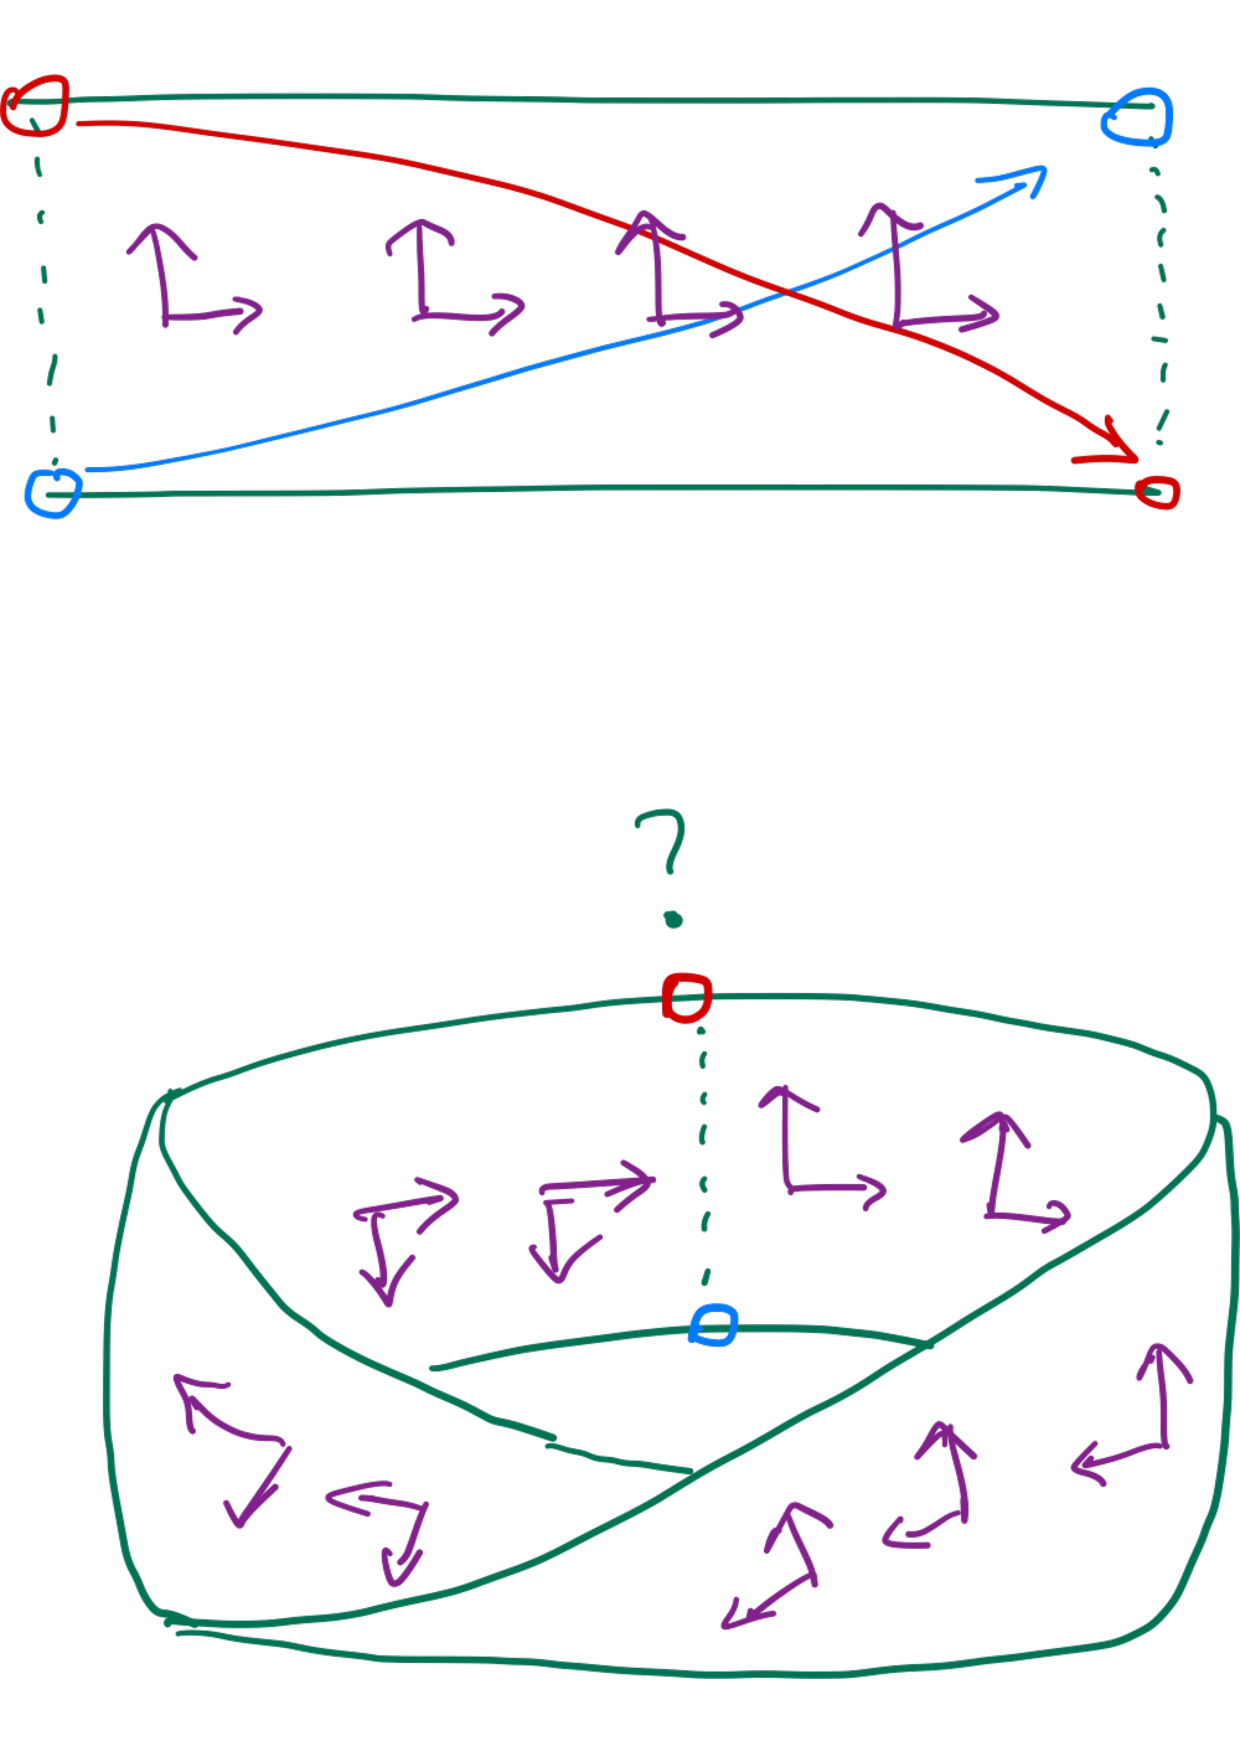
\includegraphics{7_1-mobius_strip.pdf}
\end{marginfigure}

\begin{exercise}
  Consider the open M\"obius strip $M$, a variation of Example~\ref{ex:mobius} defined as the quotient of $\R\times(-1,1)$ via the identification $(x,y) \sim (x+1, -y)$, and denote $\pi: \R\times(-1,1)\to M$ the corresponding projection map.
  The M\"obius strip inherits the differentiable structure from $\R^2$, so we need to show that there is no orientable atlas which is also compatible with the differentiable structure on $M$.
  \begin{enumerate}
    \item Define the map $\sigma:\R\times(-1,1)\to\R\times(-1,1)$ by $\sigma(x,y) = (x+1, -y)$ and show that $\pi\circ\sigma = \sigma$.
    \item If $\eta\in\Omega^2(M)$ defines\footnote{Cf. Exercise~\ref{ex:vfshape}.} $f$ by $\pi^* \eta = f \omega$ where $\omega$ is an area\footnote{I.e. a volume $2$-form.} form on $\R\times(-1,1)$.
    Show that $f(x+1, y) = - f(x,y)$.
    \item Conclude that $f$ must vanish at some point of $\R\times(-1,1)$, which implies that $M$ is non-orientable.
  \end{enumerate}
\end{exercise}

\begin{exercise}
  Let $f\in C^\infty(\R^{n+1})$ with $0$ as a regular value.
  Show that $f^{-1}(0)$ is an orientable submanifold of $\R^{n+1}$.
  %In particular, the unit $n$-sphere $\bS^n\subset\R^{n+1}$ is orientable.
\end{exercise}

\begin{exercise}\label{ex:TMorient}
  Let $M$ be a smooth manifold without boundary and $\pi: TM \to M$ its tangent bundle.
  Show that if $\{(U_\alpha,\varphi_\alpha)\}$ is any atlas on $M$, then the corresponding\footnote{Remember Theorem~\ref{thm:tgbdlsmoothmfld}.} atlas $\{(TU_\alpha, \widetilde\varphi_\alpha)\}$ on $TM$ is oriented.
  This, in particular, proves that the total space $TM$ of the tangent bundle is always orientable, regardless of the orientability of $M$.
\end{exercise}

\newthought{What about orientation on the boundaries?}
Let's first look at the tangent space. 

Let $M$ be a smooth $n$-manifold with boundary and $p\in \partial M$.
Then, we have three types of possible vectors:
\begin{enumerate}
  \item tangent boundary vectors: $X\in T_p(\partial M)\subset T_p M$ tangent to the boundary, forming an $(n-1)$-dimensional subspace of $T_p M$;
  \item inward pointing vectors: $X\in T_pM$ such that $X = \varphi^{-1}_*(Y)$ where $\varphi^{-1}: V\subset \cH^n \to M$ and $Y$ is some vector $Y = (Y_1, \ldots, Y_n)$ with $Y_n > 0$;
  \item outward pointing vectors: $X\in T_pM$ such that $-X$ is inward pointing.
\end{enumerate}
Thus, a vector field along $\partial M$ is a function $X:\partial M\to T_pM$ (not to $T_p\partial M$).

\begin{proposition}
  On a smooth manifold $M$ with boundary, there is a smooth outward pointing vector field along $\partial M$.  
\end{proposition}
\begin{proof}
  Pick an open cover of $\partial M$ with coordinate charts $\{(U_\alpha, (x^1_\alpha,\ldots,x^n_\alpha) \mid \alpha\in I\}$. Then $X_\alpha = -\frac{\partial}{\partial x^n_\alpha}$ on $U_\alpha\cap \partial M$ is smooth and outward pointing.
  Choose a partition of unity $\{\rho_\alpha \mid \alpha\in I\}$ on $\partial M$ subordinate to the open cover $\{U_\alpha\cap \partial M \mid \alpha\in I\}$.
  Then $X:= \sum_{\alpha\in I}\rho_\alpha X_\alpha$ is a smooth ouwtard pointing vector field along $\partial M$.
\end{proof}

We can use this to introduce a notion of induced orientation on $\partial M$.

\begin{proposition}
  Let $M$ be an oriented $n$-manifold with boundary.
  If $\omega$ is a volume form on $M$ and $X$ a smooth outward-pointing vector field on $\partial M$, then $\iota_X\omega$ is a smooth nowhere-vanishing $(n-1)$-form on $\partial M$ and, thus, $\partial M$ is orientable.
\end{proposition}
\begin{proof}
  Since both $\omega$ and $X$ are smooth, the contraction $\iota_X\omega$ is also smooth.
  We need to check that it cannot vanish.

  Assume that $\iota_X\omega$ does vanish at some point $p\in\partial M$, that is, $(\iota_X)(v_1, \ldots, v_{n-1}) = 0$ for all $v_1, \ldots, v_{n-1}\in T_p(\partial M)$.
  Let $\{e_1,\ldots,e_{n-1}\}$ be a basis for $T_p(\partial M)$.
  Then $\{X_p,e_1,\ldots,e_{n-1}\}$ is a basis for $T_p M$ such that
  \begin{equation}
    \omega_p(X_p, e_1, \ldots, e_{n-1}) = (\iota_X\omega)_p(e_1, \ldots, e_{n-1}) = 0.
  \end{equation}
  Then, by Exercise~\ref{ex:zeroform}, $\omega_p\equiv0$ reaching a contradiction.
  
  Therefore, $\iota_X\omega$ is non-vanishing on $\partial M$ which means that $\partial M$ is orientable.
\end{proof}

\begin{exercise}\label{ex:vfshape}
  Let $M$ be an oriented manifold with boundary, $\omega$ an orientation for $M$ and $X$ a smooth outward pointing vector field along $\partial M$.
  Prove the following statements.
  \begin{enumerate}
    \item It $\sigma$ is another orientation form on $M$, then $\sigma = f\omega$ for some everywhere positive $f\in C^\infty(M)$. Prove that  $\iota_X\sigma = f\iota_X \omega$ on $\partial M$.
    \item Show that if $Y$ is another smooth outward pointing vector field along $\partial M$, then there is an everywhere positive $f\in C^\infty(M)$ such that $\iota_Y\sigma = f \iota_X \omega$ on $\partial M$.
  \end{enumerate}
\end{exercise}

Note that if $\{(U_i, \varphi_i)\}$ is a positively oriented atlas on $M$, then $\{(U_i|_{\partial M}, \varphi_i|_{\partial M})\}$ can be negatively oriented. 
Let $\omega = dx^1\wedge\cdots\wedge dx^n$ be a positive volume form on $M$ on one of the charts, then $-\frac{\partial}{\partial x^n}$ is an outward pointing on $\partial \cH^n$ and we have\footnote{Recall Lemma~\ref{lemma:intprod}.}
\begin{align}
  \iota_{-{\partial}/\!{\partial x^n}} (dx^1\wedge\cdots\wedge dx^n)
  &= -\iota_{{\partial}/\!{\partial x^n}} (dx^1\wedge\cdots\wedge dx^n) \\
  &= -(-1)^{n-1} dx^1\wedge\cdots\wedge dx^{n-1}\wedge \iota_{{\partial}/\!{\partial x^n}} (dx^n) \\
  &= (-1)^n dx^1\wedge\cdots\wedge dx^{n-1}.
\end{align}
Thus, for example, the boundary orientation on $\partial \cH^1 = \{0\}$ is $-1$, the one on $\partial \cH^2$ is the standard orientation on $\R$ given by $dx^1$ and the one on $\partial \cH^3$ is $-dx^1\wedge dx^2$, which is the clockwise orientation in the $(x^1, x^2)$-plane, etc.

\begin{example}\label{ex:int:bdryo}
  The closed interval $[a,b]\subset\R$ with standard euclidean coordinate $x$ has a standard orientation given by the vector field $\frac{\partial}{\partial x}$. 
  Therefore\footnote{Recall the charts in Example~\ref{ex:mfldbdryinterval}.}, the boundary orientation at $b$ is $\iota_{\frac{\partial}{\partial x}}(dx) = +1$ and the one at $a$ is $\iota_{-\frac{\partial}{\partial x}}(dx) = -1$.
\end{example}

\begin{exercise}
  Orientability is common but there are many examples of nonorientable manifolds.
  \begin{enumerate}
    \item Prove that $\bS^n$ is orientable.\\
      \textit{\small Hint: above there is a small exercise that can help a lot here.}
    \item Prove that any Lie group is orientable.
    \item Prove that $\RP^n$ is orientable if and only if $n$ is odd. \\
      \textit{\small Hint: the antipodal map $x\mapsto -x$ on $\bS^n$ can help.}
  \end{enumerate}
\end{exercise}

\section{Integrals on manifolds}

To avoid unnecessary complications, we will only integrate $n$-forms with compact support.
Armed with our experience with line integrals, fond memories of multivariable analysis and our recent discoveries, we are finally ready to talk about integrals.
Let's keep things simple and go one step at a time.

\begin{definition}\label{def:intnform:chart}
  Let $M$ be a smooth $n$-manifold and $(U,\varphi)$ be a chart from an oriented atlas of $M$.
  If $\omega\in\Omega^n(M)$ be a $n$-form, $n > 0$, with compact support in $U$, we define the integral of $\omega$ as\footnote{Recall that for a diffeomorphism $\phi$, $\phi_* = (\phi^{-1})^*$.}
  \begin{equation}
    \int_M \omega = \int_U \omega := \int_{\varphi(U)} \varphi_*\omega := \int_{\R^n} \omega(x) d x^1\cdots dx^n,
  \end{equation}
  where the last is the usual Riemannian integral on $\R^n$ and, on the chart,
  \begin{equation}
    \varphi_*\omega = \omega(x)\; e^{1}\wedge \cdots\wedge e^{n}\in\Omega^n(\R^n).
  \end{equation}
  For convenience we may write $d^n x := dx^1 \cdots dx^n$.
  \marginnote[-5em]{Everything remains valid if $\R^n$ is replaced by $\cH^n$.}

  If $M$ is an oriented $0$-dimensional manifold and $f\in\Omega^0(M) = C^\infty(M)$, than we define the integral to be the sum
  \begin{equation}
    \int_M f := \sum_{p\in M} \pm f(p),
  \end{equation}
  where we take the positive sign at points where the orientation is positive and the negative sign at points where it is negative.
  The compactness assumption here implies that there are only finitely many nonzero terms in the sum.
\end{definition}

To make sure that this definition makes sense, let's show that the integral is well-defined, that is, up to orientation it does not depend on the chosen chart.

\begin{lemma}\label{lemma:intindep:chart}
  Suppose $\omega\in\Omega^n(M)$ with compact support $\supp \omega \subset U\cap V$, where $(U, \varphi)$ and $(V, \psi)$ are two positively oriented charts on the oriented manifold $M$.
  Then, the value of the integral $\int_M\omega$ is independent on the chosen chart.
\end{lemma}
\begin{proof}
  Let $\varphi$ and $\psi$ be two charts on $W = U\cap V$ with the same orientation and local coordinates $x$ and $y$, let $\sigma = \psi\circ\varphi^{-1}$ be the corresponding transition map.
  Denote, locally, $\varphi_*\omega = \omega(x) dx^1\wedge\cdots\wedge dx^n$ and $\psi_*\omega = \widetilde\omega(y) dy^1\wedge\cdots\wedge dy^n$.
  Then,
  \marginnote{Since in multivariable analysis you saw already the invariance of the Euclidean integral by orientation-preserving changes of coordinates, one could also use that directly:
  \begin{align}
    \int_{\varphi(U)} \varphi_*\omega & = \int_{\varphi(W)} \varphi_*\omega \\
    &= \int_{\sigma(\varphi(W))} \sigma_* (\varphi_*\omega) \\
    &= \int_{\psi(W)} \psi_* \omega.
  \end{align}
  }
  \begin{align}
    \int_{\varphi(W)} \varphi_*\omega &= \int \omega(x)\, d^n x \\
    &\overset{\eqref{form:cov}}{=} \int_{\varphi(W)} (\widetilde\omega \circ \sigma)(x) \det(D\sigma|_x) d^n x \\
    &\overset{(\clubsuit)}{=} \int_{\psi(W)} \widetilde\omega(y) d^n y\\
    &= \int_{\psi(W)} \psi_*\omega,
  \end{align}
  where in $(\clubsuit)$ we used the classical euclidean change of variables.
\end{proof}

To be able to integrate charts which are not supported in the domain of a single chart, we now need the help of a partition of unity.

\begin{definition}
  Let $M$ be a smooth oriented manifold and $\cA = \{(U_i,\varphi_i)\}$ a positively oriented atlas.
  If $\omega \in \Omega^n(M)$ has compact support, then the \emph{integral of $\omega$} is defined as
  \begin{equation}\label{eq:intnform}
    \int_M \omega := \sum_{j=1}^N \int_{U_j}\rho_j\omega,
  \end{equation}
  where $\{\rho_j\mid j=1,\ldots, N\}$ is a partition of unity subordinate to a finite cover\footnote{Such that $\sum_{j=1}^N \rho_j(p) = 1$ for $p\in\supp\omega$.} of $\supp \omega$ by charts domains $\{U_j\}$.
  \marginnote[-7em]{The terms on the right hand side of \eqref{eq:intnform} are all integrals as in Definition~\ref{def:intnform:chart}.}
\end{definition}

The definition above makes sense only if the value of the integral is independent of the chosen partition, but with the help of the previous lemma this is easily checked.

\begin{lemma}\label{lemma:intinman}
  The value of $\int_M\omega$ is independent from the choice of the atlas and the choice of partition of unity.
\end{lemma}
\begin{proof}
  The independence from the choice of the charts was demonstrated in Lemma~\ref{lemma:intindep:chart}.
  Let $\{\widetilde\rho_j\}$ be another partition of unity subordinate to a (possibly different) finite cover by charts $\{(V_j, \psi_j)\}$ with $\sum \widetilde\rho_j(p) = 1$ for $p\in\supp\omega$.
  Then we have,
  \begin{align}
    \sum_j \int_{\varphi_j(U_j)} (\varphi_j)_*\left(\rho_j \omega\right)
    &= \sum_j \int_{\varphi_j(U_j)} (\varphi_j)_*\left(\rho_j \sum_k \widetilde\rho_k\omega\right) \\
    &= \sum_{j,k} \int_{\varphi_j(U_j\cap V_k)} (\varphi_j)_* \left(\rho_j \widetilde\rho_k\omega\right) \\
    &\overset{(\spadesuit)}{=} \sum_{j,k} \int_{\psi_k(U_j\cap V_k)} (\psi_k)_* \left(\rho_j \widetilde\rho_k\omega\right) \\
    &= \sum_k \int_{\psi_k(V_k)} (\psi_k)_*\left(\widetilde\rho_k \sum_j\rho_j \omega\right) \\
    &= \sum_k \int_{\psi_k(V_k)} (\psi_k)_*\left( \widetilde\rho_k \omega\right),
  \end{align}
  where in $(\spadesuit)$ we used Lemma~\ref{lemma:intindep:chart}.
\end{proof}

Which immediately implies the following nice result.
\begin{theorem}[Global change of variables]\label{thm:gcv}
  Suppose $M$ and $N$ are oriented $n$-manifolds and $F:M\to N$ is an orientation preserving diffeomorphism.
  If $\omega\in\Omega^n(N)$ has compact support, then $F^*\omega$ has compact support and the following holds
  \begin{equation}
    \int_N \omega = \int_M F^* \omega.
  \end{equation}
\end{theorem}
\begin{proof}
  First of all, observe that $\supp(F^*\omega) = F^{-1}(\supp(\omega))$ which is compact since manifolds are Hausdorff spaces and $F$ is continuous.

  Let now $\{(U_i,\varphi_i)\}$ be an atlas of a positively oriented chart on $M$ and $\{\rho_i\}$ a subordinate partition of unity.
  Then, $\{(F(U_i),\varphi_i\circ F^{-1})\}$ is an atlas of positively oriented charts for $N$ and $\{\rho_i \circ F^{-1}\}$ is a partition of unity subordinate to the covering $\{F(U_i)\}$.
  By Lemma~\ref{lemma:intinman} we have,
  \begin{align}
    \int_M F^*\omega &= \sum_i \int_M \rho_i F^*\omega \\
    &= \sum_i \int_{\R^n}(\varphi_i)_*(\rho_i F^*\omega)\\
    &= \sum_i \int_{\R^n}(\varphi_i)_*(F^{-1})_*(\rho_i \circ F^{-1}) \omega \\
    &= \sum_i \int_{\R^n}(\varphi_i \circ F^{-1})_*(\rho_i \circ F^{-1}) \omega \\
    &= \int_N\omega,
  \end{align}
  which shows the commutativity of the following diagram
  \begin{equation}
    \begin{tikzcd}
      \Omega^n(M)
        \arrow[rr, "F^*", above, shift right = 0.5]
        \arrow[dr, "\int_M", below left]
        & & \Omega^n(N)
          \arrow[ll, "F_*", below, shift right = 0.5]
          \arrow[dl, "\int_N"] \\
      & \R &
    \end{tikzcd}
  \end{equation}
  and concludes the proof.
\end{proof}

This justifies the following definition.

\begin{definition}[Integral on submanifolds]\label{def:insm}
  Let $M$ an oriented smooth $m$-manifold, $N$ an oriented smooth $n$-manifold and $J:N\to M$ a smooth map\footnote{If $N\subset M$ is a submanifold, then $J:N\hookrightarrow M$ is just the inclusion map.}.
  If $\omega\in\Omega^n(M)$ restricted to $J(N)$ has compact support, we define
  \begin{equation}
    \int_N \omega := \int_N J^*\omega.
  \end{equation}
  In particular, if $M$ is compact, oriented, smooth $m$-manifold, $\omega\in\Omega^{m-1}(M)$ and $i:\partial M\hookrightarrow M$ is the inclusion of the boundary in $M$, we can interpret unambiguously
  \begin{equation}
    \int_{\partial M} \omega := \int_{\partial M} i^* \omega,
  \end{equation}
  where $\partial M$ is understood to have the induced orientation.
\end{definition}

\begin{example}\label{ex:intint}
  Let $M=[a,b]\subset \R$ equipped with the canonical global atlas $\{(M, \id_\R|_M)\}$ and $f\in C^\infty_0(M)$, i.e., smooth with compact support\footnote{Which does not mean $f(a) = f(b)=0$ since $[a,b]$ is itself compact.}.
  Then, $df\in\Omega^1(M)$ and $\supp df \subset \supp f$ is compact as well and we have
  \begin{equation}
    \int_M df = \int_a^b \frac{\partial f}{\partial x} dx = f(b)- f(a) = \int_{\partial M} f.
  \end{equation}
\end{example}

\begin{exercise}[Fubini's theorem]\label{exe:fubini}
  Let $M^m$ and $N^n$ be oriented manifolds. Endow $M\times N$ with the product orientation, that is\footnote{An equivalent way is to say that if $v_1,\ldots,v_m\in T_pM$ and $w_1, \ldots, w_n\in T_q N$ are positively oriented bases in the respective spaces, then \begin{equation}
    (v_1,0),\ldots,(v_n,0),(0,w_1), \ldots, (0,w_n)\in T_{(p,q)}(M\times N)
  \end{equation}is defined to be a positively oriented basis in the product.}, if $\pi_M : M\times N \to M$ and $\pi_N: M\times N \to N$ are the canonical projections on the elements of the product, and $\omega$ and $\eta$ respectively define orientations on $M$ and $N$, then the orientation on $M\times N$ is defined to be the orientation defined by $\pi_M^* \omega \wedge \pi_N^* \eta$.

  If $\alpha\in\Omega^m(M)$ and $\beta\in\Omega^n(N)$ have compact support, show that
  \begin{equation}
    \alpha\times\beta := (\pi_M^*\alpha)\wedge(\pi_N^*\beta)
  \end{equation}
  has compact support and is a $(m+n)$-form on $M\times N$.
  Then, prove Fubini's theorem:
  \begin{equation}
    \int_{M\times N}\alpha\times\beta = \left(\int_M\alpha\right)\left(\int_N\beta\right).
  \end{equation}
\end{exercise}

\begin{exercise}
  Let $\{e_1,\ldots,e_{n+1}\}$ be the standard basis of $\R^{n+1}$ and $\Omega_{n+1} := e_1\wedge\cdots\wedge e_{n+1}$ the induced volume form.
  On $\bS^n$ define $\omega_n\in\Omega^n(\bS^n)$ by
  \begin{equation}
    \omega_n(s)(v_1, \ldots, v_n) = \Omega_{n+1}(s, v_1, \ldots, v_n)
  \end{equation}
  for $s\in\bS^n$ and $v_1,\ldots,v_n\in T_s\bS^n$.

  In this exercise we are going to define a canonical volume $\omega_n$ on $\bS^n$ and prove that 
  \begin{equation}
    \int_{\bS^n} \omega_n = \frac{2^{m+1}\pi^m}{(2m-1)!}, \quad\mbox{if } n=2m,\; m\geq 1,
  \end{equation}
  and
  \begin{equation}
    \int_{\bS^n} \omega_n = \frac{2\pi^{m+1}}{m!}, \quad\mbox{if } n=2m+1,\; m\geq 0.
  \end{equation}

  \begin{enumerate}
    \item Show that $\omega_n$ is a volume form on $\bS^n$. In fact it is the so-called standard volume form on $\bS^n$.
    \item Let $f:\R_+\times\R^{n+1}\setminus\{0\}\to \R^{n+1}\setminus\{0\}$ be given by $f(t,s) = ts$, where $\R_+$ is defined to be the set $\{t\in\R \mid t >0\}$.
    Show that if $\R_+$ is oriented by $dt$, $\bS^n$ is oriented by $\omega_n$ and $\R^{n+1}$ is oriented by $\Omega_{n+1}$, then the Jacobian determinant $\det(Df(t,s))= t^n$.
    Conclude that $f$ is orientation preserving.
    \item Let $M$ be the annulus $M = \{x\in\R^{n+1} \mid 0<a<\|x\|<b<\infty\}$. Consider the restriction $f|_{(a,b)\times \bS^n}$ and show that for $x\in\R^{n+1}$,
    \begin{equation}
      f^*\left(e^{-\|x\|^2}\Omega_{n+1}\right) = t^n e^{-t^2}(dt \times \omega_n),
    \end{equation}
    where $dt\times\omega_n$ is a product volume form as in Exercise~\ref{exe:fubini}.
    \item Show that
    \begin{equation}
      \int_{\R^{n+1}}e^{-\|x\|^2}\Omega_{n+1} = \int_a^b t^ne^{-t^2} dt \int_{\bS^n}\omega_n.
    \end{equation}
    \item Consider the limits $a\to0^+$ and $b\to+\infty$ and show that
    \begin{equation}
      \int_0^\infty t^n e^{-t^2} dt \int_{\bS^n}\omega_n = \left(\int_{-\infty}^{+\infty} e^{-u^2} du\right)^{n+1}.
    \end{equation}
    \item Assume to know that $\int_{-\infty}^{\infty} e^{-u^2}du = \sqrt{\pi}$. Show that
    \begin{equation}
      \int_0^\infty t^{2m} e^{-t^2}dt = \frac{(2m-1)!!\sqrt{\pi}}{2^{m+1}}
      \quad\mbox{and}\quad
      \int_0^\infty t^{2m+1} e^{-t^2}dt = \frac{m!}{2},
    \end{equation}
    and use them to deduce the required formulas for $\int_{\bS^n}\omega_n$.
  \end{enumerate}
\end{exercise}

\begin{corollary}[Of Theorem~\ref{thm:gcv}]
  Let $F:M\to M$ be a diffeomorphism and $\omega\in\Omega^n(M)$ an invariant volume form, that is, $F^*\omega =\omega$.
  Then, for all compactly supported smooth functions $f\in C^\infty_0(M)$, the following holds
  \begin{equation}
    \int_M f\omega = \int_M (f\circ F)\omega.
  \end{equation}
\end{corollary}
\begin{proof}
  Follows form the previous exercise by observing
  \begin{equation}
    F^*(f\omega) = (f\circ F) F^*\omega = (f\circ F)\omega.
  \end{equation}
\end{proof}

This corollary has deep consequences in classical mechanics, which I am going to teach in the master and you are welcome to attend!

\begin{remark}
  The integral defined in this section can be extended rather immediately to measurable functions.
  Let $\omega\in\Omega^n(M)$ be a positive volume form and let $f:M\to[0,\infty)$ be measurable.
  Then one can define
  \begin{align}
    \int_M f \omega
    &= \sum_i \int_{\varphi_i(U_i)} (\varphi_i)_*(\rho_i f\omega) \\
    &= \sum_i \int_{\varphi_i(U_i)} (\rho_i f \circ\varphi_i^{-1}) (\varphi_i)_*\omega \\
    &= \sum_i \int_{\varphi_i(U_i)} (\rho_i f \circ\varphi_i^{-1})(x) \omega(x) d^n x,
  \end{align}
  where the last integral is a Lebesgue integral on $\R^n$.
  One then calls $f:M\to \R$ integrable, saying $f\in L^1(M,\omega)$, if $\int_M|f|\omega < \infty$ and defines its integral as $\int_M f\omega := \int_M f^+\omega - \int_M f^-\omega$, where $f^\pm$ denote the positive and negative components of $f$ as in the euclidean case.
\end{remark}

\section{Stokes' Theorem}

Stokes' theorem states that if $\omega$ is an $(n-1)$-form on an orientable $n$-manifold $M$, then the integral of $d\omega$ over $M$ equals the integral of $\omega$ over $\partial M$, generalising our observations for the line integral.
This is a beautiful and very important results, with deep consequences. The most immediate ones are the classical theorems of Gauss, Green and Stokes, which are just a special cases of this result.

We are going to state the theorem, discuss some of its consequences and then give its proof.

\begin{theorem}[Stokes' theorem]\label{thm:Stokes}
  Let $M$ be an oriented $n$-manifold with boundary and let $\omega\in\Omega^{n-1}(M)$ be compactly supported.
  Then,
  \begin{equation}\label{eq:Stokes}
    \int_M d\omega = \int_{\partial M} \omega.
  \end{equation}
  \marginnote[-4.5em]{Here, $\partial M$ inherits the orientation from $M$ as in Definition~\ref{def:insm}, $\omega$ on the right-hand side is interpreted as $i^*\omega$ where $i:\partial M \hookrightarrow M$ is the inclusion of the boundary and if $\partial M =\emptyset$ then the right-hand side is interpreted as $0$.}
\end{theorem}

\marginnote[1em]{On a similar note, the fact that $dd\omega =0$ for every $\omega\in\Lambda^n(M)$ corresponds to the fact that a boundary has no boundary, that is $\partial\partial M = \emptyset$ for any $M$: indeed, for any $\omega\in\Lambda^n(M)$ one has \begin{equation}
  0=\int_M dd\omega = \int_{\partial M}d\omega = \int_{\partial\partial M} \omega.
\end{equation}}
\begin{corollary}
  Let $M$ be an oriented $n$-manifold without boundary and let $\omega\in\Omega^{n-1}(M)$ be compactly supported.
  Then,
  \begin{equation}
    \int_M d\omega = 0.
  \end{equation}
  That is, the integral of a compactly supported exact form over a manifold without boundary vanishes.
\end{corollary}

\begin{corollary}
  Let $M$ be a compact oriented $n$-manifold with boundary and let $\omega\in\Omega^{n-1}(M)$ be closed.
  Then,
  \begin{equation}
    \int_{\partial M} \omega = 0.
  \end{equation}
  That is, the integral of a closed form on the boundary of a compact manifold vanishes.
\end{corollary}

\begin{corollary}
  Let $M$ a smooth $m$-manifold, $N$ an oriented smooth $n$-manifold and $J:N\to M$ a smooth map\footnote{If $N\subset M$ is a submanifold, then $J:N\hookrightarrow M$ is just the inclusion map.}.
  If $\omega\in\Omega^{n-1}(M)$ restricted to $J(N)$ has compact support, then
  \begin{equation}
    \int_{N} d J^*\omega = \int_{\partial N} J^*\omega,
  \end{equation}
  where $\partial N$ inherits the orientation of $N$.
\end{corollary}

\begin{corollary}[Green's theorem]
  Suppose $D$ is a compact regular domain in $\R^2$ and $P,Q\in C^\infty(D)$, then
  \begin{equation}
    \int_D \left(\frac{\partial Q}{\partial x} - \frac{\partial P}{\partial y}\right)dxdy = \int_{\partial D}(Pdx + Qdy).
  \end{equation}
\end{corollary}

\begin{remark}
  The requirement of compactness in Stokes' theorem may seem there just to avoid technicalities involving the convergence of the integral, however, it also avoid subtleties due to the boundary as shown in the following example.
  Let $M=(a,b)$, thus $\partial M = \emptyset$, and $f(x)=x$.
  Then,
  \begin{equation}
    b-a = \int_a^b df \neq \int_{\partial M} f = 0.
  \end{equation}
  But this does not contradict Stokes' theorem since $f$ is not compactly supported.

  If you close the interval, then $f$ becomes with compact support and we are back in the case of Example~\ref{ex:intint} where we had already seen Stokes' theorem.
\end{remark}

\begin{proof}
  \newthought{Part I: euclidean boundary case}.
  Let's start with a special case: suppose $M = \cH^n$ itself.
  Since $\omega$ has compact support, there is $R > 0$ such that $\supp \omega \subset A = [-R,R]^{n-1}\times[0,R]$ is enclosed within the rectangle $A$.
  We can write $\omega$ in standard coordinates to get
  \begin{equation}
    \omega = \sum_{j=1}^n \omega^j dx^1 \wedge \cdots\wedge \widehat{dx}^j \wedge \cdots\wedge dx^n
  \end{equation}
  where the hat means that the corresponding element $dx^j$ is omitted.
  Therefore\footnote{Exercise: explicitly write down the steps of the computation.},
  \begin{equation}
    d\omega = \sum_{j=1}^n (-1)^{j-1} \frac{\partial \omega^j}{\partial x^j}dx^1\wedge\cdots\wedge dx^n,
  \end{equation}
  and we end up with the integral
  \begin{align}
    \int_{\cH^n} d\omega
    &= \sum_{j=1}^n (-1)^{j-1} \int_A\frac{\partial \omega^j}{\partial x^j}dx^1\wedge\cdots\wedge dx^n \\
    &= \sum_{j=1}^n (-1)^{j-1} \int_0^R\int_{-R}^R\cdots\int_{-R}^{R}\frac{\partial \omega^j}{\partial x^j}(x) d^n x. %d x^1\cdots dx^n.
  \end{align}
  The last are genuine euclidean integrals and we can change the order of integration in each term to always integrate the $x^j$ term first.
  The usual euclidean fundamental theorem of calculus then, for the terms with $j\neq n$, implies
  \begin{align}
    \int_{\cH^n} d\omega
    &= \sum_{j=1}^n (-1)^{j-1} \int_0^R\int_{-R}^R\cdots\int_{-R}^{R}\frac{\partial \omega^j}{\partial x^j}(x) d^n x \\ %dx^1\cdots dx^n \\
    &=\sum_{j=1}^n (-1)^{j-1} \int_0^R\int_{-R}^R\cdots\int_{-R}^{R}\frac{\partial \omega^j}{\partial x^j}(x) dx^j dx^1\cdots\widehat{dx^j}\cdots dx^n \\
    &=\sum_{j=1}^n (-1)^{j-1} \int_0^R\int_{-R}^R\cdots\int_{-R}^{R}\omega^j(x) \Big|_{x^j=-R}^{x^j=R} dx^1\cdots\widehat{dx^j}\cdots dx^n \\
    &= 0
  \end{align}
  since $R$ is larger than the support of $\omega$ at each coordinate.
  The only term that may not be zero is the $j=n$ one.
  In that case, for the same reasons,
  \begin{align}
    \int_{\cH^n} d\omega
    &=(-1)^{n-1} \int_{-R}^R\int_{-R}^R\cdots\int_{-R}^R\int_{0}^{R}\frac{\partial \omega^n}{\partial x^j}(x) dx^n d^{n-1} x \\ %dx^1\cdots dx^{n-1} \\
    &=(-1)^{n-1} \int_{-R}^R\int_{-R}^R\cdots\int_{-R}^R \omega^n(x)\Big|_{x^n=0}^{x^n=R} dx^n d^{n-1} x \\ %dx^1\cdots dx^{n-1} \\
    &=(-1)^{n-1} \int_{-R}^R\int_{-R}^R\cdots\int_{-R}^R \omega^n(x^1, \ldots, x^{n-1}, 0) d^{n-1} x %dx^1\cdots dx^{n-1}.
    .\label{eq:lhsHn}
  \end{align}
  We now need to compare this with the right-hand side of~\eqref{eq:Stokes}.
  To this end, compute he following
  \begin{equation}
    \int_{\partial \cH^n}\omega = \sum_{j=1}^n \int_{A\cap\cH^n} \omega_j(x^1, \ldots, x^{n-1}, 0) dx^1 \wedge \cdots\wedge \widehat{dx}^j \wedge \cdots\wedge dx^n.
  \end{equation}
  Since $x^n$ vanishes on $\partial\cH^n$, the pullback of $dx^n$ to the boundary is zero, and thus the only surviving term in the sum is the last one, that is,
  \begin{equation}\label{eq:rhsHn}
    \int_{\partial \cH^n}\omega = \int_{A\cap\cH^n} \omega_n(x^1, \ldots, x^{n-1}, 0) dx^1 \wedge\cdots\wedge dx^{n-1}.
  \end{equation}
  Since coordinates $(x^1, \ldots, x^{n-1})$ are positively oriented for $\cH^n$ when $n$ is even and negatively oriented when $n$ is odd, we obtain the equality of \eqref{eq:lhsHn} and \eqref{eq:rhsHn}.

  \newthought{Part II: euclidean case}.
  If $M=\R^n$ the considerations above apply without the need to make an exception for the case $j=n$, so all the terms vanish on the left-hand side of~\eqref{eq:Stokes} while the right-hand side is trivially zero due to the empty boundary.

  \newthought{Part III: ``arbitrary'' $M$ but $\supp\omega$ is contained in a single chart}.
  Let $(U,\varphi)$ denote a chart such that $\supp \omega \subset U$.
  Without loss of generality assume that $\varphi$ is a positively oriented boundary chart, then
  \begin{align}
    \int_M d\omega
    &= \int_{\cH^n}(\phi^{-1})^* dw \\
    &= \int_{\cH^n} d\left((\phi^{-1})^* \omega\right) \\
    &\overset{(\spadesuit)}{=} \int_{\partial \cH^n}(\phi^{-1})^* w \\
    &= \int_{\partial M} w , 
  \end{align}
  where in the $(\spadesuit)$ step we applied the computations above and where $\partial \cH^n$ has the orientation induced by $\cH^n$.
  For a negatively oriented smooth boundary chart, the computation applies with an extra negative sign on each side of the equation.
  For an interior chart, we get the same computations with $\R^n$ in place of $\cH^n$.

  \newthought{Part IV: ``arbitrary'' $M$ and $\omega$}.
  Let finally $\omega\in\Omega^{n-1}(M)$ with compact support.
  Without loss of generality, let $\{(U_i, \varphi_i)\mid i\in I\}$ be a finite cover of $\supp \omega$ by positively oriented charts and $\{\rho_i\}$ a subordinate partition of unity with $\sum \rho_i(p) = 1$ for all $p\in\supp \omega$.
  Then, by applying the previous arguments for each $i$ we get
  \begin{align}
    \int_{\partial M} \omega
    &= \sum_i \int_{\partial M} \rho_i\omega
     = \sum_i \int_M d(\rho_i \omega) \\
    &= \sum_i \int_M (d\rho_i \wedge\omega + \rho_i\, d\omega) \\
    &= \int_M d\left(\sum_i \rho_i\right)\wedge\omega + \int_M \left(\sum_i \rho_i\right) d\omega \\ 
    &= 0 + \int_M d\omega,
  \end{align}
  concluding the proof.
\end{proof}

\begin{exercise}
  Let $D^n := \{x=(x^1, \ldots, x^n)\in\R^n \mid \|x\| \leq 1\}$ denote the unit disk in $\R^n$ centred at $0$. Recall that $\partial D^n = \bS^{n-1}$.
  \begin{enumerate}
    \item Compute $\int_{\bS^1} \eta$ where $\eta$ is the following 1-form on $\R^2$: $\eta = -x^2 dx^1 + x^1 dx^2$.
    \item Compute $\int_{\bS^2} \omega$ where $\omega$ is the following 2-form on $\R^3$: $\omega = -x^1 dx^1\wedge dx^3 - x^2 dx^1\wedge dx^3 + x^3 dx^1\wedge dx^2$.
    \item Show that $\eta$ and $\omega$ above are closed but not exact (as differential forms on $\bS^1$ and $\bS^2$ respectively).
  \end{enumerate}
  \textit{\small Hint: if you look carefully, you may notice that you don't really need to write anything down in coordinates.}
\end{exercise}

\begin{example}
  Consider the annulus $M=\{(x,y)\in\R^2 \mid 1/2\leq x^2+y^2 \leq 1\}$ and the $1$-form $\omega = \frac{-y dx + x dy}{x^2 + y^2} = d\theta$ where $(x,y) = (\rho\cos\theta, \rho\sin\theta)$.
  
  Then $d\omega = 0$ and therefore $\int_M d\omega = 0$.
  Furthermore,
  \begin{marginfigure}
    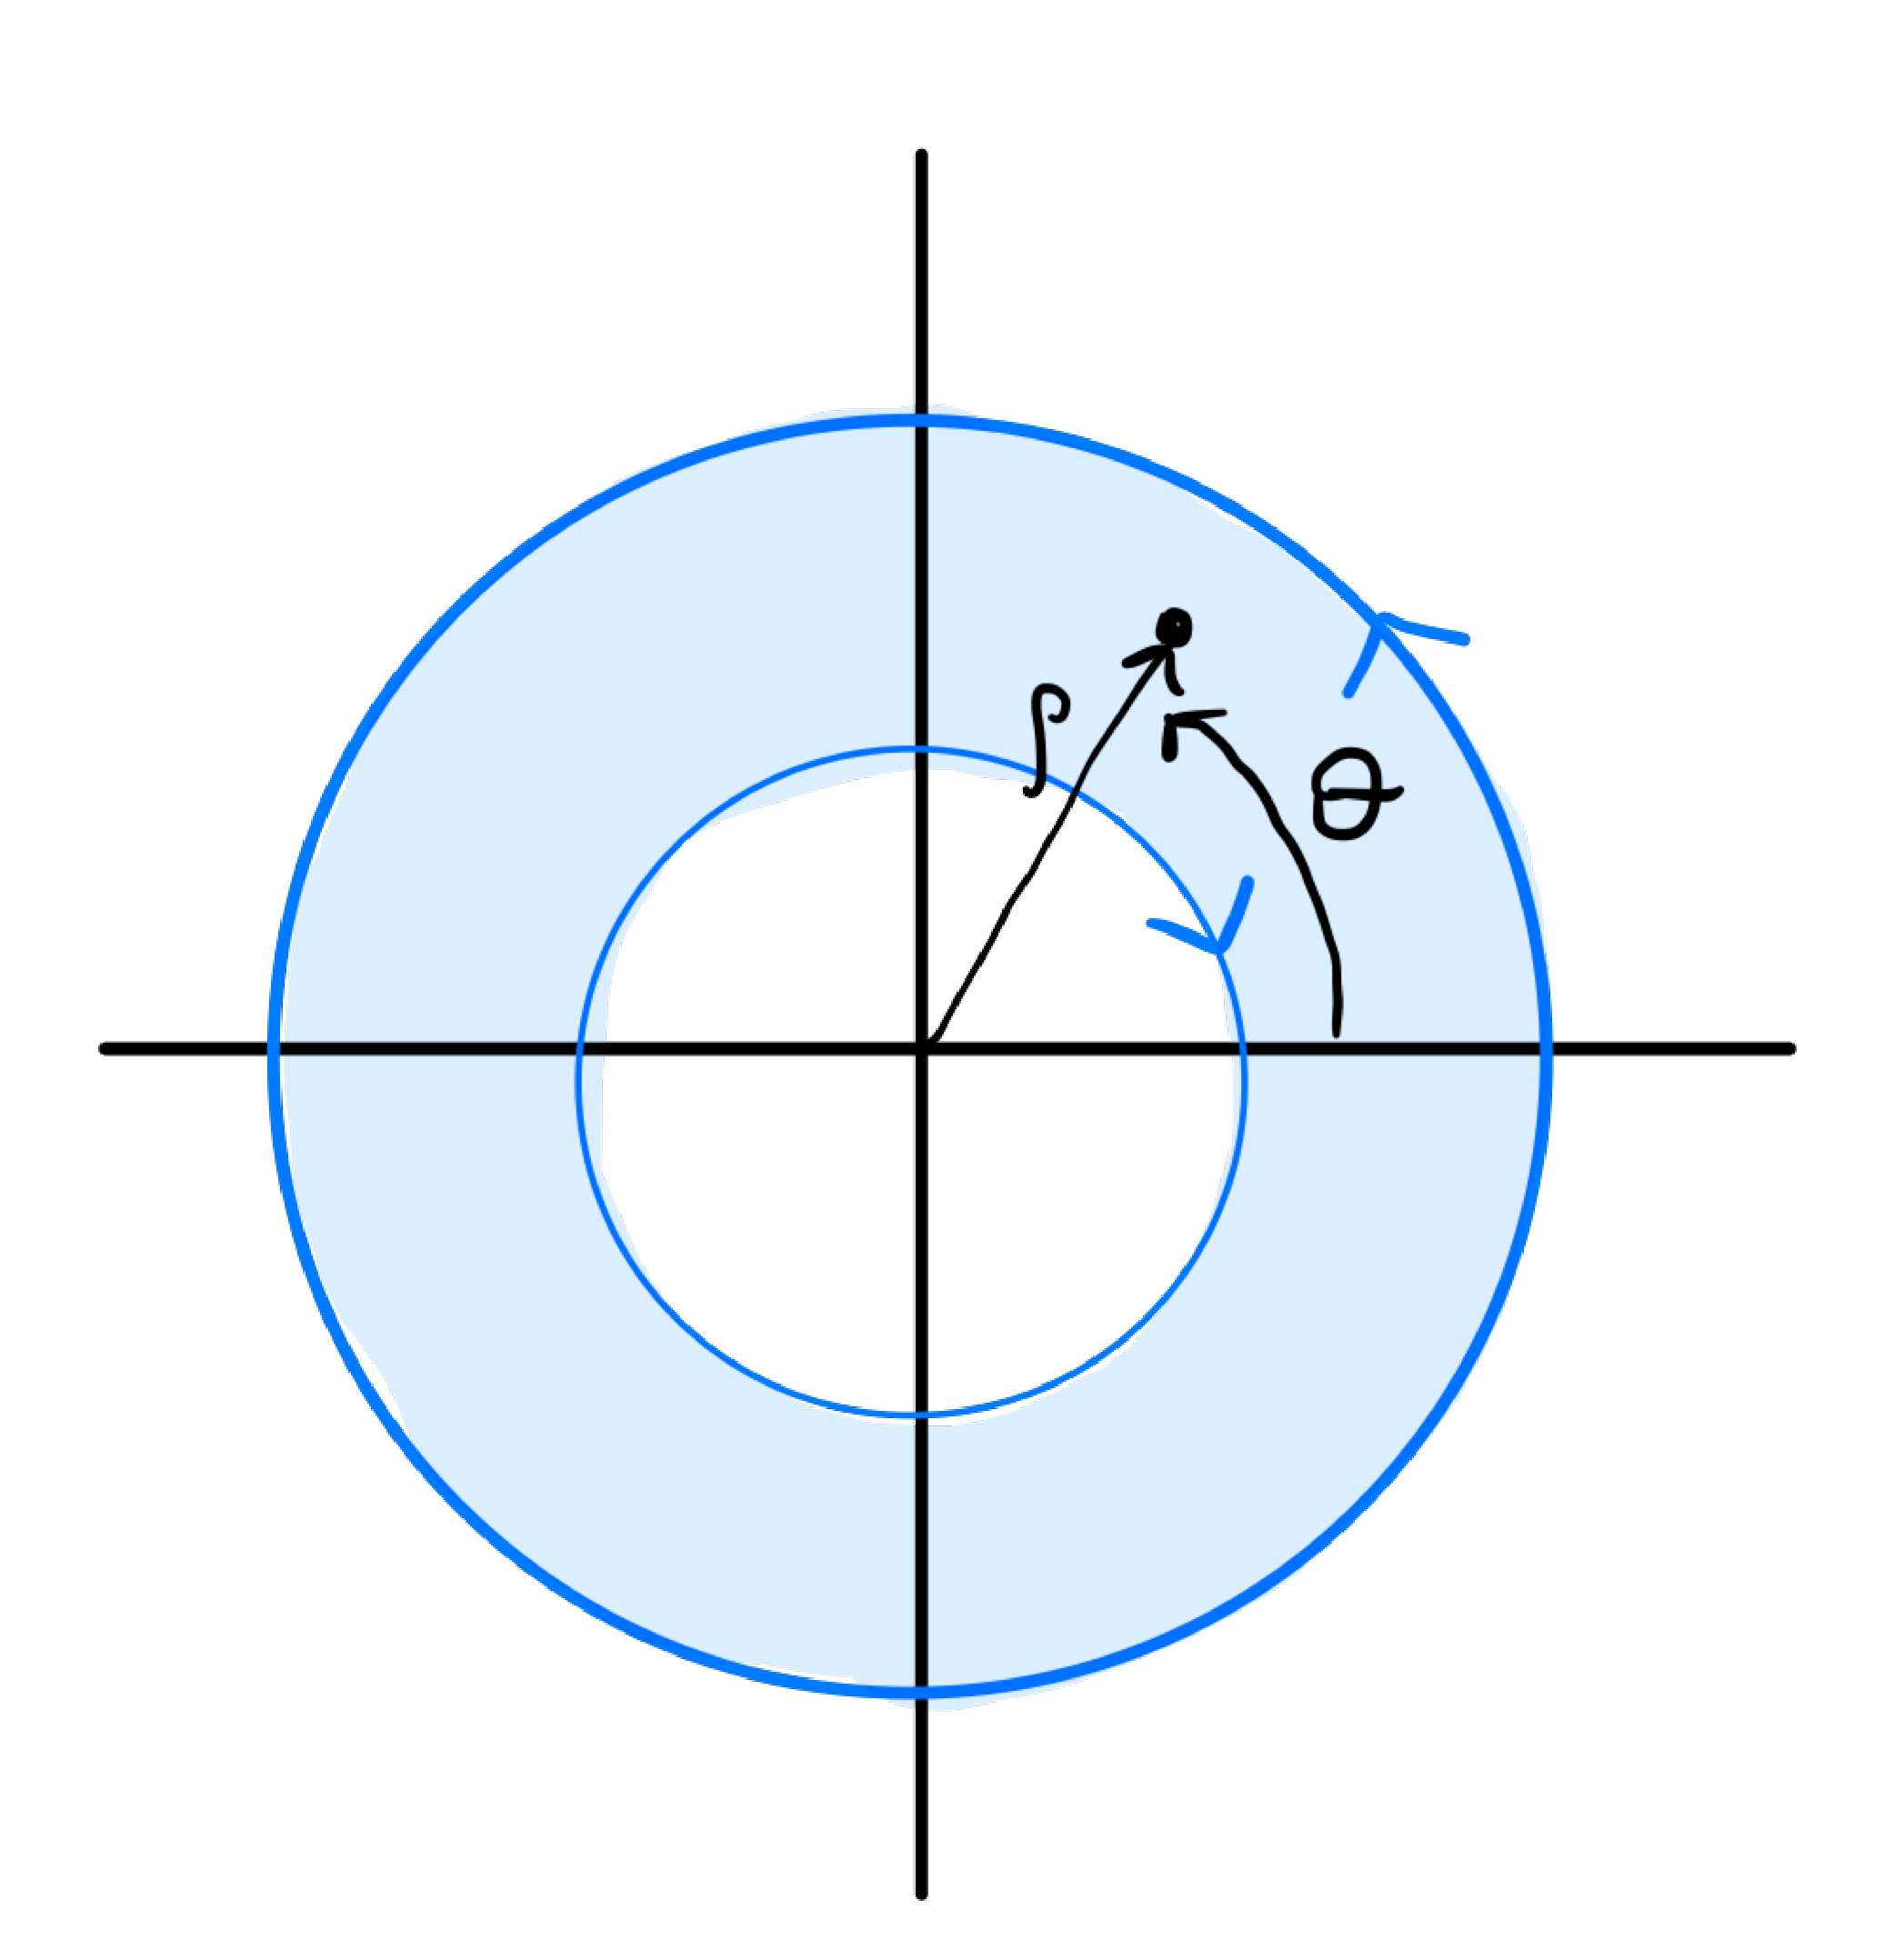
\includegraphics{8_3_8-annulus.pdf}
  \end{marginfigure}
  \begin{align}
    \int_{\partial M}\omega
    &= \int_{x^2 + y^2 =1} \omega + \int_{x^2+y^2 =1/2}\omega \\ 
    &= \int_{0}^{2\pi} d\theta - \int_0^{2\pi}d \theta \\
    &= 2\pi - 2\pi = 0.
  \end{align}

  An important consequence of this is that while locally $\omega$ is the differential of the angle function $\theta$, this cannot be exact on all $M$: indeed, if $\omega = d\eta$ for some $\eta$, we would have
  \begin{equation}
    2\pi = \int_{\bS^1}\omega = \int_{\bS^1}d\eta \overset{!}{=} \int_{\partial\bS^1}\eta = 0.
  \end{equation}

  Moreover, since $2\pi = \int_{\bS^1}\omega$, Stokes' theorem also implies that $\bS^1$ is not the boundary of a compact regular domain in $\R^2\setminus\{0\}$.
\end{example}

In fact this example is a particular case of the following corollary of Stokes' theorem.

\begin{corollary}
  Suppose $M$ is a smooth $m$-manifold with or without boundary,$N\subseteq M$ is an oriented compact smooth $n$-submanifold (without boundary) and $\omega$ is a closed $n$-form on $M$.
  If $\int_N\omega \neq 0$ then the following are true:
  \begin{enumerate}
    \item $\omega$ is not exact on $M$;
    \item $N$ is not the boundary of an oriented compact smooth submanifold with boundary in $M$.
  \end{enumerate}
\end{corollary}
\begin{exercise}
  Prove this corollary. \\
  \textit{\small Hint: follows from two the previous corollaries.}
\end{exercise}


\begin{exercise}
In this problem we are going to prove the smooth version of Brouwer's fixed point theorem.
  
\begin{theorem}[Brouwer's fixed point theorem (smooth version)]\label{thm:bfp1}
  Let $D_n:=\{x\in\mathbb{R}^n\;\mid\;\|x\|\leq 1\}$ denote the closed unit disk in $\mathbb{R}^n$. % and $\mathbb{S}^{n-1} = \partial D_n$ its boundary, the $(n-1)$-sphere.
  Any smooth map $g: D_n \to D_n$ has a fixed point, that is, $\exists\,p\in D_n$ such that $g(p) = p$.
\end{theorem}

We will proceed by first showing another result.

\begin{theorem}\label{thm:bfp2}
  Let $N$ be a compact $n$-dimensional submanifold of $\mathbb{R}^n$ with non-empty boundary $\partial N$.
  Then, there is no differentiable map $f: N \to \partial N$ for which every boundary point is a fixed point, that is, for which $f(p) = p$ for all $p\in\partial N$.
\end{theorem}

Let $\Omega = dx^1 \wedge \cdots\wedge dx^n$ denote the standard volume form on $N$, that is, the restriction of the standard volume form on $\mathbb{R}^n$ to $N$,
and $X$ be an outward-pointing vector field on $\partial N$.
%Finally, let $i:\partial N\hookrightarrow N$ be the inclusion map.

\begin{enumerate}
  \item Show that $\omega = \iota_X \Omega$ is a closed non-vanishing form on $\partial N$.
  \item Show that $f^*\omega$ is closed.
  \item Prove Theorem~\ref{thm:bfp2}.\\\textit{Hint: assume there is $f$ such that $f(p)=p$ for all $p\in \partial N$ and use integration to get a contradiction.}
  \item Prove Theorem~\ref{thm:bfp1}.\\\textit{Hint: by contradiction, use the half line from $p$ to $g(p)$ to construct a function for which every point in the boundary is fixed. }
\end{enumerate}
\end{exercise}


\begin{appendices}

\chapter{Frobenius theorem}
Integrable and nonintegrable distributions, Contact geometry, Frobenius theorem.

\chapter{Vector bundles and connections}
Hopefully we can cut on differential forms since they were treated in multivariable analysis and get to this.

\end{appendices}

% \begin{appendices}
%   \chapter{Solution to selected exercises}
%   \section{Chapter~\ref{ch:manifolds}}
  
%   \newthought{Exercise~\ref{exe:rntopsp}.}
%   \begin{enumerate}
%     \item[] Hausdorff. For $x\neq y\in\R^n$, let $\epsilon = d(x,y)/3$.
%     Then the two balls $B_x(\epsilon) := \{z\in X \;\mid\; d(z,x)<\epsilon\}$ and $B_y(\epsilon)$ are disjoint open sets containing $x$ and $y$ respectively.
%     \item[] Second countable. As countable basis for the topology we can take the open balls $B_\epsilon(x)$ with rational radii $\epsilon\in\Q$ and centers $x\in\Q^n$.
%   \end{enumerate}
  
% \end{appendices}

\printbibliography
\addcontentsline{toc}{chapter}{Bibliography}
\end{document}